% A LaTeX template for MSc Thesis submissions to 
% Politecnico di Milano (PoliMi) - School of Industrial and Information Engineering
%
% S. Bonetti, A. Gruttadauria, G. Mescolini, A. Zingaro
% e-mail: template-tesi-ingind@polimi.it
%
% Last Revision: October 2021
%
% Copyright 2021 Politecnico di Milano, Italy. NC-BY

\documentclass{Configuration_Files/PoliMi3i_thesis}

%------------------------------------------------------------------------------
%	REQUIRED PACKAGES AND  CONFIGURATIONS
%------------------------------------------------------------------------------

% CONFIGURATIONS
\usepackage{parskip} % For paragraph layout
\usepackage{setspace} % For using single or double spacing
\usepackage{emptypage} % To insert empty pages
\usepackage{multicol} % To write in multiple columns (executive summary)
\setlength\columnsep{15pt} % Column separation in executive summary
\setlength\parindent{0pt} % Indentation
\raggedbottom  

% PACKAGES FOR TITLES
\usepackage{titlesec}
% \titlespacing{\section}{left spacing}{before spacing}{after spacing}
\titlespacing{\section}{0pt}{3.3ex}{2ex}
\titlespacing{\subsection}{0pt}{3.3ex}{1.65ex}
\titlespacing{\subsubsection}{0pt}{3.3ex}{1ex}
\usepackage{color}

% PACKAGES FOR LANGUAGE AND FONT
\usepackage[english]{babel} % The document is in English  
\usepackage[utf8]{inputenc} % UTF8 encoding
\usepackage[T1]{fontenc} % Font encoding
\usepackage[11pt]{moresize} % Big fonts

% PACKAGES FOR IMAGES
\usepackage{graphicx}
\usepackage{transparent} % Enables transparent images
\usepackage{eso-pic} % For the background picture on the title page
\usepackage{subfig} % Numbered and caption subfigures using \subfloat.
\usepackage{tikz} % A package for high-quality hand-made figures.
\usetikzlibrary{}
\graphicspath{{./Images/}} % Directory of the images
\usepackage{caption} % Coloured captions
\usepackage{xcolor} % Coloured captions
\usepackage{amsthm,thmtools,xcolor} % Coloured "Theorem"
\usepackage{float}
\usepackage{svg}

% STANDARD MATH PACKAGES
\usepackage{amsmath}
\usepackage{amsthm}
\usepackage{amssymb}
\usepackage{amsfonts}
\usepackage{bm}
\usepackage[overload]{empheq} % For braced-style systems of equations.
\usepackage{fix-cm} % To override original LaTeX restrictions on sizes

% PACKAGES FOR TABLES
\usepackage{tabularx}
\usepackage{longtable} % Tables that can span several pages
\usepackage{colortbl}
\usepackage{booktabs}

% PACKAGES FOR ALGORITHMS (PSEUDO-CODE)
\usepackage{algorithm}
\usepackage{algorithmic}

% PACKAGES FOR REFERENCES & BIBLIOGRAPHY
\usepackage[colorlinks=true,linkcolor=black,anchorcolor=black,citecolor=black,filecolor=black,menucolor=black,runcolor=black,urlcolor=black]{hyperref} % Adds clickable links at references
\usepackage{cleveref}
\usepackage[square, numbers, sort&compress]{natbib} % Square brackets, citing references with numbers, citations sorted by appearance in the text and compressed
\bibliographystyle{abbrvnat} % You may use a different style adapted to your field

% OTHER PACKAGES
\usepackage{pdfpages} % To include a pdf file
\usepackage{afterpage}
\usepackage{lipsum} % DUMMY PACKAGE
\usepackage{fancyhdr} % For the headers
\fancyhf{}
\usepackage{tikz}
\usetikzlibrary{decorations.markings}

% Input of configuration file. Do not change config.tex file unless you really know what you are doing. 
% Define blue color typical of polimi
\definecolor{bluepoli}{cmyk}{0.4,0.1,0,0.4}

% Custom theorem environments
\declaretheoremstyle[
  headfont=\color{bluepoli}\normalfont\bfseries,
  bodyfont=\color{black}\normalfont\itshape,
]{colored}


% Set-up caption colors
\captionsetup[figure]{labelfont={color=bluepoli}} % Set colour of the captions
\captionsetup[table]{labelfont={color=bluepoli}} % Set colour of the captions
\captionsetup[algorithm]{labelfont={color=bluepoli}} % Set colour of the captions

\theoremstyle{colored}
\newtheorem{theorem}{Theorem}[chapter]
\newtheorem{proposition}{Proposition}[chapter]

% Enhances the features of the standard "table" and "tabular" environments.
\newcommand\T{\rule{0pt}{2.6ex}}
\newcommand\B{\rule[-1.2ex]{0pt}{0pt}}

% Pseudo-code algorithm descriptions.
\newcounter{algsubstate}
\renewcommand{\thealgsubstate}{\alph{algsubstate}}
\newenvironment{algsubstates}
  {\setcounter{algsubstate}{0}%
   \renewcommand{\STATE}{%
     \stepcounter{algsubstate}%
     \Statex {\small\thealgsubstate:}\space}}
  {}

% New font size
\newcommand\numfontsize{\@setfontsize\Huge{200}{60}}

% Title format: part 
\titleformat{\part}[block]{
    \thispagestyle{empty}
    \AddToShipoutPicture*{\BackgroundPic} % TODO: remove?
    \centering\fontsize{40}{20}\selectfont\bfseries}{\textcolor{bluepoli}
    {Part   \thepart\hsp\hspace{5mm}}\textcolor{bluepoli}{| }\hsp}{1pt}
{\Huge\bfseries\textcolor{bluepoli}
}

% Title format: chapter
\titleformat{\chapter}[hang]{
\fontsize{50}{20}\selectfont\bfseries\filright}{\textcolor{bluepoli} \thechapter\hsp\hspace{2mm}\textcolor{bluepoli}{|   }\hsp}{0pt}{\huge\bfseries \textcolor{bluepoli}
}

% Title format: section
\titleformat{\section}
{\color{bluepoli}\normalfont\Large\bfseries}
{\color{bluepoli}\thesection.}{1em}{}

% Title format: subsection
\titleformat{\subsection}
{\color{bluepoli}\normalfont\large\bfseries}
{\color{bluepoli}\thesubsection.}{1em}{}

% Title format: subsubsection
\titleformat{\subsubsection}
{\color{bluepoli}\normalfont\large\bfseries}
{\color{bluepoli}\thesubsubsection.}{1em}{}

% Shortening for setting no horizontal-spacing
\newcommand{\hsp}{\hspace{0pt}}

\makeatletter
% Renewcommand: cleardoublepage including the background pic
\renewcommand*\cleardoublepage{%
  \clearpage\if@twoside\ifodd\c@page\else
  \null
  \AddToShipoutPicture*{\BackgroundPic}
  \thispagestyle{empty}%
  \newpage
  \if@twocolumn\hbox{}\newpage\fi\fi\fi}
\makeatother

%For correctly numbering algorithms
\numberwithin{algorithm}{chapter}

%----------------------------------------------------------------------------
%	NEW COMMANDS DEFINED
%----------------------------------------------------------------------------

% EXAMPLES OF NEW COMMANDS
\newcommand{\bea}{\begin{eqnarray}} % Shortcut for equation arrays
\newcommand{\eea}{\end{eqnarray}}
\newcommand{\e}[1]{\times 10^{#1}}  % Powers of 10 notation

%----------------------------------------------------------------------------
%	ADD YOUR PACKAGES (be careful of package interaction)
%----------------------------------------------------------------------------

%----------------------------------------------------------------------------
%	ADD YOUR DEFINITIONS AND COMMANDS (be careful of existing commands)
%----------------------------------------------------------------------------

%----------------------------------------------------------------------------
%	BEGIN OF YOUR DOCUMENT
%----------------------------------------------------------------------------

\begin{document}

\fancypagestyle{plain}{%
\fancyhf{} % Clear all header and footer fields
\fancyhead[RO,RE]{\thepage} %RO=right odd, RE=right even
\renewcommand{\headrulewidth}{0pt}
\renewcommand{\footrulewidth}{0pt}}

%----------------------------------------------------------------------------
%	TITLE PAGE
%----------------------------------------------------------------------------

\pagestyle{empty} % No page numbers
\frontmatter % Use roman page numbering style (i, ii, iii, iv...) for the preamble pages

\puttitle{
	title = Nonlinear Whole-Body Force Control of a Smart E-Cargo, % Title of the thesis
	name = Davide Barbone, % Author Name and Surname
	course = Mechanical Engineering - Ingegneria Meccanica, % Study Programme (in Italian)
	ID  = 991995,  % Student ID number (numero di matricola)
	advisor={Prof. Francesco Braghin, Dr. Daniele Pucci}, % Supervisor name
	coadvisor={Dr. Stefano Dafarra, Dr. Silvio Traversaro}, % Co-Supervisor name, remove this line if there is none
	academicyear={2023-24},  % Academic Year
} % These info will be put into your Title page 

%----------------------------------------------------------------------------
%	PREAMBLE PAGES: ABSTRACT (inglese e italiano), EXECUTIVE SUMMARY
%----------------------------------------------------------------------------
\startpreamble
\setcounter{page}{1} % Set page counter to 1

% ABSTRACT IN ENGLISH
\chapter*{Abstract} 
\label{ch:Abstract}

% ABSTRACT IN ENGLISH

Since their introduction, Segway-like vehicles have attracted significant interest from manufacturers and users, due to their simple mechanical structure, unique maneuverability, and ability to operate in different scenarios, with a wide range of possible applications. Despite the apparent simplicity of the model, studying the controllers to be applied to these vehicles is not straightforward given their particular nonlinear dynamics and inherent instability. 

Over the years, various control strategies have been developed for these vehicles, ranging from more classical methodologies to the application of intelligent controllers, demonstrating good results in terms of performance. However, less emphasis has been placed on studying slip prevention between wheels and terrain and on utilizing these vehicles as platforms capable of autonomous navigation.

The aim of this thesis is to address these two challenges, applied to an autonomous two-wheeled electric cargo (smart E-Cargo) with a Task Space Inverse Dynamics (TSID) controller.
This controller, within an optimization problem, is capable of managing a series of kinematic and dynamic constraints to ensure pure rolling motion, while simultaneously guaranteeing self-balancing and tracking of a desired trajectory in space. Since TSID is mainly designed for humanoid robots modeled as floating-base systems, the same approach has been adopted for the smart E-Cargo.

The proposed control strategy has been implemented using Matlab and Simulink, receiving in input a Unified Robot Description Format (URDF) model of the vehicle. Simulation results demonstrate the effectiveness of the TSID approach in maintaining stability and achieving precise control. Additionally, robustness analysis is conducted to evaluate the performance under various load conditions and uncertainties in the friction coefficient estimation.
\\
\textbf{Keywords:} Segway, control, TSID , friction, self-balancing, tracking % Keywords 


% ABSTRACT IN ITALIAN
\chapter*{Sintesi} 
\label{ch:Sintesi}

 Sin dalla loro introduzione, i veicoli di tipo segway hanno attirato un notevole interesse da parte di produttori e utenti, grazie alla loro semplice struttura meccanica, manovrabilità unica e capacità di operare in diversi scenari, con una vasta gamma di possibili applicazioni. Nonostante la semplicità apparente del modello, studiare i controllori da applicare a questi veicoli non è semplice data la loro particolare dinamica non lineare e intrinseca instabilità.

Nel corso degli anni, sono state sviluppate diverse strategie di controllo per questi veicoli, spaziando dalle metodologie più classiche all'applicazione di controllori intelligenti,mostrando buoni risultati in termini di performance. Tuttavia, si è prestata meno attenzione allo studio della prevenzione dello slittamento tra ruote e terreno e all'utilizzo di questi veicoli come piattaforme capaci di navigazione autonoma.

Lo scopo di questa tesi è affrontare queste due sfide, applicate a un veicolo elettrico autonomo a due ruote (smart E-Cargo), mediante un controllore Task Space Inverse Dynamics (TSID). Questo controllore, all'interno di un problema di ottimizzazione, è in grado di gestire una serie di vincoli cinematici e dinamici per garantire un moto di puro rotolamento, assicurando allo stesso tempo l'auto-bilanciamento e il tracking di una traiettoria desiderata nello spazio. Poiché il TSID è principalmente progettato per robot umanoidi modellati come sistemi floating base, lo stesso approccio è stato adottato per l'E-Cargo.

La strategia di controllo proposta è stata implementata utilizzando Matlab e Simulink a partire da un modello del veicolo nel formato Unified Robot Description Format (URDF). I risultati delle simulazioni mostrano l'efficacia dell'approccio TSID nel mantenere la stabilità e nel raggiungere un tracking preciso. Inoltre, è stata condotta un'analisi di robustezza per valutare le prestazioni sotto diverse condizioni di carico e in presenza di un'incertezza nella misura dell'attrito.
\\
\textbf{Parole chiave:} Segway, controllo, TSID , attrito, auto-bilanciamento, tracciamento % Parole chiave 


% List of acronyms
% List of acronyms
\chapter*{List of Acronyms}
\label{ch:List_of_acronyms}
Here the list of the acronyms adopted.

\begin{table}[h]
    \centering
    \caption{List of Acronyms used throughout the thesis.}
    \renewcommand{\arraystretch}{1.5} % Increase the vertical spacing between rows
    \begin{tabular}{@{}l@{\hspace{3cm}}l@{}}
    \toprule
    \textbf{Acronym} & \textbf{Description} \\
    \midrule
    BLDC  & Brushless Direct Current \\
    CoM  & Center of Mass \\
    DoF & Degrees of Freedom \\
    ECLSP & Equality-Constrained Least-Squares Problem \\
    EoM & Equation of Motion \\
    FC & Fuzzy Logic \\
    FLC & Feedback Linearization Control \\
    LSP & Least-Squares Problem \\
    MIMO & Multi Input Multi Output \\
    OCT & Optimal Control Theory \\
    ODE & Ordinary Differential Equation \\
    PI & Proportional-Integral \\
    QP & Quadratic Program \\
    TSID & Task Space Inverse Dynamics \\
    TWIP & Two Wheeled Inverted Pendulum \\
    URDF & Unified Robot Description Format \\
    \bottomrule
    \end{tabular}
\end{table}


% List of symbols
% LIST OF SYMBOLS
% Write out the List of Symbols in this page

\chapter*{List of Symbols}
\label{ch:List_of_symbols}
Here the list of the symbols adopted.

\begin{table}[h]
    \centering
    \caption{List of Symbols used throughout the thesis.}
    \renewcommand{\arraystretch}{1.5} % Increase the vertical spacing between rows
    \begin{tabular}{@{}l@{\hspace{3cm}}l@{}}
    \toprule
    \textbf{Symbols} & \textbf{Description} \\
    \midrule
    ${A,B}$  & coordinate frames \\
    ${\mathbf{p}}$ & arbitrary point \\
    ${\mathbf{o}_B}$  & origin of $B$ \\
    ${[A]}$ & orientation frame associated to [A] \\
    ${B[A]}$  & frame with origin $\mathbf{o}_B$ and orientation $A$ \\
    ${{}^{A}\mathbf{p}}$ & coordinates of $\mathbf{p}$ w.r.t. $A$ \\
    ${{}^{A}\mathbf{o}_B}$  & coordinates of $\mathbf{o}_B$ w.r.t. $A$ \\
    ${{}^{A} H_B}$  & homogeneous transformation from $B$ to $A$ \\
    ${{}^{A} X_B}$  & velocity transformation from $B$ to $A$ \\
    ${}^{C} \mathbf{v}_{A,B}$  & 6D velocity expressing the velocity of $B$ w.r.t. A written in $C$ \\
    ${}^{C} \mathbf{v}^{\wedge{}}_{A,B}$  & 4 x 4 matrix representation of ${}^{C} \mathbf{v}_{A,B}$  \\
    ${}^{C} \mathbf{v}_{A,B}\times$  & 6 x 6 matrix representation of the 6D velocity cross product  \\
    ${}^{C}J_{A,B}$  & Jacobian relating the velocity of $B$ w.r.t. $A$ expressed in C \\
    ${}^{C}J_{A,B/F}$  & Jacobian relating the velocity of $B$ w.r.t. $A$ expressed in $C$, \\ & where the moving-base velocity is expressed in $F$ \\
     \bottomrule
    \end{tabular}
\end{table}




%----------------------------------------------------------------------------
%	LIST OF CONTENTS/FIGURES/TABLES/SYMBOLS
%----------------------------------------------------------------------------

% TABLE OF CONTENTS
\thispagestyle{empty}
\tableofcontents % Table of contents 
\thispagestyle{empty}
\cleardoublepage

%-------------------------------------------------------------------------
%	THESIS MAIN TEXT
%-------------------------------------------------------------------------
% In the main text of your thesis you can write the chapters in two different ways:

\addtocontents{toc}{\vspace{2em}} % Add a gap in the Contents, for aesthetics
\mainmatter % Begin numeric (1,2,3...) page numbering

% --------------------------------------------------------------------------
% NUMBERED CHAPTERS % Regular chapters following
% --------------------------------------------------------------------------

\part{Background}\label{part:background}
\chapter{Rigid Multibody Dynamics}
\label{ch:chapter_one}%
% The \label{...}% enables to remove the small indentation that is generated, always leave the % symbol.

In this chapter, we introduce some useful information regarding rigid multibody dynamics.

\section{Notation overview}
\label{sec:Notation_overview}

Throughout this thesis, according to the work of Traversaro \cite{Traversaro2017thesis} we adhere to the following notation and conventions.

\begin{itemize}
    \item The set of real numbers is denoted by $\mathbb{R}$. Let $ \mathbf{u}$ and $ \mathbf{v}$ be two $n$-dimensional column vectors of real numbers, i.e. $ \mathbf{u},  \mathbf{v} \in \mathbb{R}^n$, then their inner product is denoted as $ \mathbf{u}^T  \mathbf{v}$, with "$T$" the transpose operator.
    \item The identity matrix of dimension $n$ is denoted $ {I}_n \in \mathbb{R}^{n\times n}$; the zero column vector of dimension $n$ is denoted $ \mathbf{0}_n \in \mathbb{R}^n$; the zero matrix of dimension $n\times m$ is denoted $ {0}_{n\times m} \in \mathbb{R}^{n\times m}$.
    \item The set $SO(3)$ is the set of $\mathbb{R}^{3\times 3}$ orthogonal matrices with determinant equal to one, that is,
    \begin{equation}
    SO(3) := \{  {R} \in \mathbb{R}^{3\times 3} \,|\,  {R}^T  {R} =  {I}_3, \det( {R}) = 1 \}.
    \end{equation}
    \item The set $\mathfrak{so}(3)$, read \textit{little} $\mathfrak{so}(3)$, is the set of $3\times 3$ skew-symmetric matrices,
    \begin{equation}
    \mathfrak{so}(3) := \{  {S} \in \mathbb{R}^{3\times 3} \,|\,  {S}^T = - {S} \}.
    \end{equation}
    \item The set $SE(3)$ is defined as
    \begin{equation}
    SE(3) := \left\{ \begin{pmatrix}  {R} &  \mathbf{p} \\  \mathbf{0}_3^T & 1 \end{pmatrix} \in \mathbb{R}^{4\times 4} \,|\,  {R} \in SO(3),  \mathbf{p} \in \mathbb{R}^3 \right\}.
    \end{equation}
    \item The set $\mathfrak{se}(3)$ is defined as
    \begin{equation}
    \mathfrak{se}(3) := \left\{ \begin{pmatrix} \Omega & \mathbf{v} \\  \mathbf{0}_{3}^T & 0 \end{pmatrix} \in \mathbb{R}^{4\times 4} \,|\, \Omega \in \mathfrak{so}(3), \mathbf{v} \in \mathbb{R}^3 \right\}.
    \end{equation}
    \item Given the vector ${\bm{\omega}} = (x; y; z) \in \mathbb{R}^3$, we define $\bm{\omega}^\wedge$ (read $\bm{\omega}$ \textit{hat}) as the $3\times 3$ \textit{skew-symmetric matrix}
    \begin{equation}
     {\bm{\omega}}^\wedge = \begin{Bmatrix} x\\ y \\ z \end{Bmatrix}^\wedge := \begin{bmatrix} 0 & -z & y \\ z & 0 & -x \\ -y & x & 0 \end{bmatrix} \in so(3).
    \end{equation}
    Given the \textit{skew-symmetric matrix} $W = \bm{\omega}^\wedge$, we define $ {W}^\vee \in \mathbb{R}^{3}$ (read $W$ \textit{vee} ) as
    \begin{equation}
     {W}^\vee = \begin{bmatrix} 0 & -z & y \\ z & 0 & -x \\ -y & x & 0 \end{bmatrix}^\vee:= \begin{Bmatrix} x \\ y \\ z \end{Bmatrix} \in \mathbb{R}^3.
    \end{equation}
    Clearly, the vee operator is the inverse of the hat operator.
    \item Given a vector $\mathbf{v} = (\bm{v}; \bm{\omega}) \in \mathbb{R}^6$, $\bm{v}$ and $\bm{\omega} \in \mathbb{R}^3$, we define
    \begin{equation}
    \mathbf{v}^\wedge = \begin{Bmatrix} \bm{v} \\ \bm{\omega} \end{Bmatrix}^\wedge := \begin{bmatrix} \bm{\omega}^\wedge & \bm{v} \\  0_{1 \times 3} & 0 \end{bmatrix} \in se(3).
    \end{equation}
    Similarly to what is done for vectors in $\mathbb{R}^3$ above, we define the \textit{vee} operator as the inverse of the hat operator such that
    \begin{equation}
    \begin{bmatrix} \bm{\omega}^\wedge & \bm{v} \\  \mathbf{0}_{3}^{T} & 0 \end{bmatrix}^\vee := \begin{Bmatrix} \bm{v} \\ \bm{\omega} \end{Bmatrix} =  \mathbf{v} \in \mathbb{R}^3
    \end{equation}
\end{itemize}

    \section{Coordinate frames and transformations}
    \label{sec:Coordinate frames and transformations}

    We opt to employ a representation method that utilizes homogeneous matrices to describe the relative configuration (translation and rotation) of two coordinate frames in three-dimensional space. Homogeneous matrices possess the advantage of being globally continuous and are easy to perform calculations with, utilizing basic matrix multiplication.
   
    Given two frames $A$ and $B$, the coordinate transformation from $B$ to $A$ will be denoted as:
    \begin{equation}
    {}^{A} {R}_B \in SO(3).
    \end{equation}
    This coordinate transformation ${}^{A} {R}_B$ is independent of the positions of the origins of the two frames and only depends on their relative orientation. \\
    
    Given two frames $A$ and $B$, the position and orientation of the frame $B$ with respect to $A$ will be denoted by the $4 \times 4$ homogeneous matrix
    \begin{equation}
    {}^{A} {H}_B := \begin{bmatrix}
    {}^{A} {R}_B & {{}^{A} \mathbf{o}_B} \\
     {0}_{1 \times 3} & 1 \\
    \end{bmatrix} \in \mathbb{R}^{4 \times 4}.
    \label{eq:Homogeneous transformation}
    \end{equation}

    We can use the matrix defined in Equation \eqref{eq:Homogeneous transformation} to describe the coordinate transformation between two frames given a point $ {p}$:
    starting from the classical coordinate transformation equation:
    \begin{equation}
    {}^{A} \mathbf{p} = {}^{A} {R}_B {}^{B} \mathbf{p} + {{}^{A} \mathbf{o}_B}.
    \label{eq:coordinate transformation}
    \end{equation}

    in homogeneous coordinates, denoted ${}^{A}\bar{ {p}} := ({}^{A} {p};1) \in \mathbb{R}^{4}$, and likewise for ${}^{B}\bar{ {p}}$  it becomes:
    \begin{equation}
    {}^{A}\bar{ \mathbf{p}} = {}^{A} {H}_B {}^{B}\bar{ \mathbf{p}}.
    \label{eq:homogeneous coordinate transformation}
    \end{equation}

    This property of defining a coordinate transformation by a simple matrix multiplication can be used for various purposes. Knowing the relative homogeneous matrix between two coordinate frames means that quantities computed numerically in one of these frames can be transformed to the other by a matrix multiplication. Furthermore, when rigid bodies are moving over time, their motion can be described by a time-varying homogeneous matrix, which can also be used to describe the time-evolution of the position of any point attached to the body by a matrix multiplication.

    \section{Rigid body velocity}
    \label{sec:Rigid body velocity}

    After defining all the important quantities to identify the position and orientation of frames, the next aspect is to provide definitions of its velocities.
    Given a point $ {p}$ and a frame $A$, we define:
    \begin{equation}
    {}^{A}\dot{ \mathbf{p}} := \frac{d}{dt}({}^{A} \mathbf{p}).
    \end{equation}

    Starting from this definition we write also:

    \begin{equation}
    {}^{A}\dot{ \mathbf{o}}_B := \frac{d}{dt}({}^{A} \mathbf{o}_B).
    \end{equation}

    \begin{equation}
    {}^{A}\dot{ {R}}_B := \frac{d}{dt}({}^{A} {R}_B).
    \end{equation}

    Now, since we want to use a time varying homogeneous matrix $ {H}(t)$ to describe the position and orientation of a rigid body, it is straightforward to use 
    \begin{equation}
    {}^{A}\dot{ {H}}_B := \frac{d}{dt}({}^{A} {H}_B) = \begin{bmatrix}
    {}^{A}\dot{ {R}}_B & {}^{A}\dot{ \mathbf{o}}_B \\
     \mathbf{0}_{3}^{T} & 0 \\
    \end{bmatrix} \quad \text{with} \quad  {R}(t) {R}^{T}(t) =  {R}^{T}(t) {R}(t) =   {I}   \end{equation}
    to describe its velocity.
    However, at all times the matrix $ {H}(t)$ is constrained to be a homogeneous matrix, and so also the degrees of freedom of $\dot{ {H}}(t)$ are constrained, depending on the current value of $ {H}(t)$.

    If we compute the time derivative of the constraint on $ {R}$, it results in:
    \begin{equation}
    \mathbf{0} = \dot{ {R}}^{T} {R} +  {R}^{T}\dot{ {R}} = ( {R}^{T}\dot{ {R}})^{T} +  {R}^{T}\dot{ {R}}.
    \label{eq:skewsymmetric R}
    \end{equation}

    Equation \eqref{eq:skewsymmetric R} shows that the constraints on $\dot{ {H}}$ can be translated into the constraint that $ {R}^{T}\dot{ {R}}$ must be a skew-symmetric matrix, and the bottom row of $\dot{ {H}}$ must be all zeros; this leads  to the notion of  a twist to represent the velocity of a rigid body.

    \subsection{Twists}
    \label{subsec: Twists}
    A \textit{twist} is an element of $\mathfrak{se}(3)$, given as the result of the multiplication of ${}^{A}\dot{ {H}}_B$ by the inverse of ${}^{A} {H}_B$ on the left or on the right.

    Multiplying on the left, one obtains

    \begin{equation}
    {}^{A} {H}^{-1}_B{}^{A}\dot{ {H}}_B = \begin{bmatrix}
    {}^{A} {R}^{T}_B & -{}^{A} {R}^{T}_B{}^{A} \mathbf{o}_B \\
     {0}_{1 \times 3} & 1 \\
    \end{bmatrix} \begin{bmatrix}
    {}^{A}\dot{ {R}}_B & {}^{A}\dot{ \mathbf{o}}_B \\
     {0}_{1 \times 3} & 0 \\
    \end{bmatrix} = \begin{bmatrix}
    {}^{A} {R}^{T}_B{}^{A}\dot{ {R}}_B & {}^{A} {R}^{T}_B{}^{A}\dot{ \mathbf{o}}_B \\
     {0}_{1 \times 3} & 0 \\
    \end{bmatrix}.
    \label{eq: twist derivation}
    \end{equation}
    
    At this point we can define the following quantities: ${}^{B}\bm{v}_{A,B}, {}^{B}\bm{\omega}_{A,B} \in \mathbb{R}^3 \quad \text{so that}$

    \begin{equation}
    {}^{B}\bm{v}_{A,B} := {}^{A} {R}^{T}_B{}^{A}\dot{ \mathbf{o}}_B.
    \end{equation}

    \begin{equation}
    {}^{B}\bm{\omega}^{\wedge}_{A,B} := {}^{A} {R}^{T}_B{}^{A}\dot{ {R}}_B.
    \end{equation}

    The \textit{left trivialized} velocity of frame $B$ with respect to frame $A$ is then defined as 
    \begin{equation}
    {}^{B} \mathbf{v}_{A,B} := \begin{Bmatrix} {}^{B}\bm{v}_{A,B} \\ {}^{B}\bm{\omega}_{A,B} \end{Bmatrix} \in \mathbb{R}^6.
    \label{eq: Left trivialized veocity}
    \end{equation}

    and then by construction:

    \begin{equation}
    {}^{B} \mathbf{v}^{\wedge}_{A,B} = {}^{A} {H}^{-1}_B {}^{A}\dot{ {H}}_B.
    \label{eq: twist definition}
    \end{equation}

    Similarly to what is done in Equation \eqref{eq: twist derivation}, multiplying ${}^{A}\dot{ {H}}_B$ by the inverse of ${}^{A} {H}_B$ on the right we obtain

    \begin{equation}
    {}^{A}\dot{ {H}}_B{}^{A} {H}^{-1}_B = \begin{bmatrix}
    {}^{A}\dot{ {R}}_B & {}^{A}\dot{ \mathbf{o}}_B \\
     {0}_{1 \times 3} & 0 \\
    \end{bmatrix} \begin{bmatrix}
    {}^{A} {R}^{T}_B & -{}^{A} {R}^{T}_B{}^{A} \mathbf{o}_B \\
     {0}_{1 \times 3} & 1 \\
    \end{bmatrix}  = \begin{bmatrix}
    {}^{A}\dot{ {R}}_B{}^{A} {R}^{T}_B & {}^{A}\dot{ \mathbf{o}}_B -  {}^{A}\dot{ {R}}_B{}^{A} {R}^{T}_B{}^{A} \mathbf{o}_B \\
     {0}_{1 \times 3} & 0 \\
    \end{bmatrix}
    \end{equation}
    
    At this point we can define the following quantities: ${}^{A}\bm{v}_{A,B}, {}^{A}\bm{\omega}_{A,B} \in \mathbb{R}^3 \quad \text{so that}$


    \begin{equation}
    {}^{A}\bm{v}_{A,B} := {}^{A}\dot{ \mathbf{o}}_B -  {}^{A}\dot{ {R}}_B{}^{A} {R}^{T}_B{}^{A} \mathbf{o}_B.
    \end{equation}

    \begin{equation}
    {}^{A}\bm{\omega}^{\wedge}_{A,B} := {}^{A}\dot{ {R}}_B{}^{A} {R}^{T}_B.
    \end{equation}

    The \textit{right trivialized} velocity of frame $B$ with respect to frame $A$ is then defined as 
    
    \begin{equation}
    {}^{A} \mathbf{v}_{A,B} := \begin{Bmatrix} {}^{A}\bm{v}_{A,B} \\ {}^{A}\bm{\omega}_{A,B} \end{Bmatrix} \in \mathbb{R}^6
    \label{eq: Right trivialized veocity}
    \end{equation}

    and then by construction:

    \begin{equation}
    {}^{A} \mathbf{v}^{\wedge}_{A,B} = {}^{A}\dot{ {H}}_B{}^{A} {H}^{-1}_B.
    \end{equation}

    \textit{Left trivialized} velocities and \textit{right trivialized} velocities are related via a linear transformation ${}^{A}X_B$ defined as:

    \begin{equation}
    {}^{A} {X}_B := \begin{bmatrix}
    {}^{A} {R}_B & {}^{A} \mathbf{o}^{\wedge}_B{}^{A} {R}_B \\
     {0}_{3 \times 3} & {}^{A} {R}_B\\
    \end{bmatrix} \in \mathbb{R}^{6 \times 6}
    \end{equation} 

    and the relation is the following

    \begin{equation}
    {}^{A} \mathbf{v}_{A,B} := {}^{A} {X}_B {}^{B} \mathbf{v}_{A,B}.
    \end{equation} 

    The inverse transformation is simply given by ${}^{B} {X}_A$
    We have defined \textit{left trivialized} and \textit{right trivialized} velocities, but they are special cases of a general idea of expressing relative velocity between two frames, in any arbitrary frame.

    For this purpose we define

    \begin{equation}
    {}^{C} \mathbf{v}_{A,B} := \begin{Bmatrix} {}^{C}\bm{v}_{A,B} \\ {}^{C}\bm{\omega}_{A,B} \end{Bmatrix} \in \mathbb{R}^6.
    \end{equation}

    which can be linearly related to both \textit{left trivialized} and \textit{right trivialized} velocities as

    \begin{equation}
    {}^{C} \mathbf{v}_{A,B} := {}^{C} {X}_A {}^{A} \mathbf{v}_{A,B} = {}^{C} {X}_B {}^{B} \mathbf{v}_{A,B}.
    \end{equation}

    The whole description provided in this section is necessary to understand the following concept:
    none of the previously defined $twists$ is sufficient to give us information about what we can call the \textit{natural velocities} of a frame, that are respectively ${}^{A} {\dot{o}}_B$ and ${}^{A}\bm{\omega}_{A,B}$ \cite{Traversaro-Saccon}, that in many cases are needed for example to apply feedback control strategies.

    At this purpose we define the \textit{mixed velocity} of frame B with respect to
    frame A (we call it mixed as it has both the flavor of a left trivialized velocity due
    to the linear velocity part and of a right trivialized velocity due to the angular
    velocity part) as:

    \begin{equation}
    {}^{B[A]} \mathbf{v}_{A,B} = {}^{B[A]} {X}_B {}^{B} \mathbf{v}_{A,B} = \begin{bmatrix} 
    {}^{A} {R}_B & 0 \\
    0 & {}^{A} {R}_B \\
    \end{bmatrix} \begin{bmatrix} 
    {}^{A} {R}_B {}^{A}\dot{ \mathbf{o}}_B \\
    {}^{A}\bm{\omega}_{A,B} \\
    \end{bmatrix} = \begin{Bmatrix} 
    {}^{A}\dot{ \mathbf{o}}_B \\
    {}^{A}\bm{\omega}_{A,B} \\
    \end{Bmatrix}. 
    \end{equation}

    \section{Frame acceleration}
    \label{sec:Frame acceleration}
    
    In the robotics literature, frame accelerations are defined in several ways, and here are provided the most commonly adopted interpretations. With reference to \cite{Traversaro-Saccon} we start from the most trivial one that we call \textit{apparent acceleration} of a frame $B$ with respect to a frame $A$ expressed in a frame C: it is simply the time derivative of the corresponding velocity ${}^{C} \mathbf{v}_{A,B}$ 

    \begin{equation}
    {}^{C}\dot{ \mathbf{v}}_{A,B} := \frac{d}{dt} ({}^{C} \mathbf{v}_{A,B}).
    \label{eq: Apparent acceleration}
    \end{equation}

    By recalling the definition for the left trivialized velocity in Equation \eqref{eq: Left trivialized veocity} we can write:

    \begin{equation}
    {}^{C}\dot{ \mathbf{v}}_{A,B} := \frac{d}{dt} ({}^{C} {X}_{B}{}^{B} \mathbf{v}_{A,B}) = {}^{C} {X}_{B} {}^{B} {\dot{\mathbf{v}}}_{A,B} + {}^{C} {\dot{X}}_{B}{}^{B} \mathbf{v}_{A,B}.
    \label{eq: Acceleration transformation}
    \end{equation}

    Equation \eqref{eq: Acceleration transformation} shows that in general ${}^{C}\dot{ \mathbf{v}}_{A,B} \neq {}^{C} {X}_{B} {}^{B} {\dot{\mathbf{v}}}_{A,B}$ because this equation is true only if frame $C = A$.
    
    The same property holds for right trivialized velocities with the only difference that in this case $C = B$.

    Starting from these considerations it is possible to define the (intrinsic) \textit{acceleration} of a frame $B$ with respect to a frame $A$ expressed in a frame $C$ as:

    \begin{equation}
    {}^{C} \mathbf{a}_{A,B} := {}^{C} {X}_{A} {}^{A} {\dot{\mathbf{v}}}_{A,B} = {}^{C} {X}_{B}{}^{B} {\dot{\mathbf{v}}}_{A,B}.
    \label{eq: Intrinsic acceleration}
    \end{equation}
 
    In our analysis, we use the following (mixed) apparent acceleration, which is commonly employed in robotics and is defined as

    \begin{equation}
    {}^{B[A]}\dot{ \mathbf{v}}_{A,B} = \begin{Bmatrix}
    {}^{B[A]}\dot{\bm{v}}_{A,B} \\
    {}^{B[A]}\dot{\bm{\omega}}_{A,B}
    \end{Bmatrix} = \begin{Bmatrix}
    {}^{A}  {\ddot{\mathbf{o}}}_{B} \\
    {}^{A}\dot{\bm{\omega}}_{A,B}.
    \end{Bmatrix}
    \label{eq: Mixed apparent acceleration}
    \end{equation}

    The reason is that the linear acceleration corresponds to the Cartesian acceleration of the origin of $B$ with respect to frame $A$

    \section{Force-Torque covectors}
    \label{sec:Force-Torque covectors}
    
    The force acting on a rigid body is defined as a stacking of the linear component $\bm{f} \in \mathbb{R}^{3}$ and the angular component $ \bm{\tau} \in \mathbb{R}^{3}$ of the wrench acting on the body. In particular, we can define $ \mathbf{f} \in \mathbb{R}^6$ with respect to a frame $B$ as:

    \begin{equation}
    {}_{B} \mathbf{f} = 
    \begin{Bmatrix}
    {}_{B}\bm{f} \\
    {}_{B}\bm{\mu}
    \end{Bmatrix}.
    \label{eq: Wrench definition}
    \end{equation}

    A change of reference frame can be expressed as:

    \begin{equation}
    {}_{A} \mathbf{f} = {}^{A} {X}_{B} {}_{B} \mathbf{f},
    \end{equation}

    in which

    \begin{equation}
    {}_{A} {X}^{B} = {}^{B} {X}_{A}^{T}
    \label{eq: Forces transformation matrix}
    \end{equation}
    
    is the 6D forces transformation matrix defined as:

    \begin{equation}
    \begin{bmatrix}
    {}^{A} {R}_{B} &  {0}_{3\times3} \\
    {}^{A} \mathbf{o}^{\wedge}_{B} {}^{A} {R}_{B} & {}^{A} {R}_{B}
    \end{bmatrix}.
    \end{equation}

    It is important to realize that Equation \eqref{eq: Forces transformation matrix} ensures the following power identity holds:

    \begin{equation}
    \langle {}_{B} \mathbf{f}, {}^{B} \mathbf{v}_{A,B} \rangle = \langle {}_{A} \mathbf{f}, {}^{A} \mathbf{v}_{A,B} \rangle,
    \end{equation}
    
    where $ \mathbf{f}$ can be interpreted as a $6D$ force applied to a rigid body to which the moving frame $B$ is rigidly attached, and $A$ is the absolute inertial frame.

    \section{Multibody Systems Modelling}
    \label{sec:Multibody Systems Modelling}

    In this section, we provide a brief overview of the derivation of mechanical systems' equations of motion (EoM). We begin by defining a multibody system and describing its characteristics. We then proceed to derive the EoM for floating-base multibody systems using the Lagrangian approach, which is the method utilized in this thesis.

    According to \cite{Flores}, a general multibody system has two main characteristics:

    \begin{enumerate}
    \item \textbf{Mechanical components} that describe large translational and rotational displacements .
    \item \textbf{Kinematic joints} that impose some constraints or restrictions on the relative motion of the bodies.
    \end{enumerate}
    
    In the end it can be considered as a collection of rigid and/or flexible bodies interconnected by kinematic joints and possibly some force elements.
    We start providing some definiton for both links and joints:
    
    \subsection{Links and Joints}
    \label{subsec: Links and Joints}

    We describe the robot as being composed of $n + 1$ rigid bodies, called \textit{links}, connected by $n$ \textit{joints}, each with a single degree of freedom. Instead of using the real models of the links and joints, we will use their ideal approximations, which can be summarized in the following definitions \cite{Duindam-phd-thesis}:


    \begin{description}
        \item[] \textbf{Ideal Link}: it is defined as a finite volume of point masses, all of which have fixed relative distances, so they are not subject to deformation.
        \item[] \textbf{Ideal Joint}: is defined as a constraint between two rigid links that allows
        only certain relative velocities and prevents others, independently of the forces and torques applied to the links.        
    \end{description}

    In general ideal joints can allow from 0 (fixed joint) to 6 (universal joint) \textbf{DoF} and are defined by a "joint \textit{axis}", but without loss of generality we will consider only 1-\textbf{DoF} joints, in particular only \textit{revolute} joints \cite{Traversaro2017thesis}:

    A \textbf{Revolute Joint} with an \textit{axis} $\mathbf{a} \in \mathbb{R}^3, |\mathbf{a}| =1$ that connects two bodies $B$ and $D$, with  ${}^{B}H_{D} (0) = 1_4$ , is responsible for the following joint transform: 

    \begin{equation}
         {}^{B}H_{D}(\theta) = \begin{bmatrix}
             {}^{B}R_{D}(\theta) & \mathbf{0}_{3 \times 1} \\
             0_{1 \times 3} & 1 \\
         \end{bmatrix} , {}^{B}R_{D}(\theta) = 1_3 + \cos(\theta)\mathbf{a}^{\wedge} + \sin(\theta)(\mathbf{a}^{\wedge})^2
    \label{eq: Revolute joint transformation}
    \end{equation}

    \subsection{Floating-Base generalized coordinates}
    \label{subsec: Floating-Base generalized coordinates}

    Following \cite{Marion-et-al.}, \textbf{generalized coordinates} are described as: \textit{any set of quantities that completely specifies the state of a system}

    Before entering in the details, here can be introduced a general notation that will be employed troughout all the chapters:
    $A$ will denote an $inertial frame$ and $B$ the $moving-base$ frame representing a frame rigidly attached to one of the bodies composing the multibody system, selected to express the the relative pose of the system with respect to the inertial frame $A$.
    
    For moving-base multibody systems, the \textit{configuration} is parametrized as: $ \mathbf{q} = ( {H},  \mathbf{s}) \in SE(3) \times \mathbb{R}^{n_j}$ , with $ {H} = {}^{A} {H}_{B} \in SE(3)$ representing the pose (position and orientation) of the moving-base frame $B$ and $ \mathbf{s} \in \mathbb{R}^{n_J}$ the internal joint displacements ($ {s}$ stands for shape).

    The dimension of $ \mathbf{q}$ is: $\mathbb{R}^{3} \times SO(3) \times \mathbb{R}^{n_j}$, where $SO(3)$ is a non-minimal coordinates representation,.
    This can be parametrized in several ways (Euler angles, axis-angle, Cardano angles) to obtain a minimal coordinates representation. This parametrization makes the moving-base $B$ a fictitious 6-\textbf{DoF} joint constituted by 3 prismatic joints connecting $B$ with $A$ and three rotational ones.
    This setup leads to floating-base systems always being \textbf{underactuated} because these additional 6 \textbf{DoF} are non-actuated, leaving the base non-actuated.

    The velocity of a floating-base multibody system has instead a different structure \cite{Traversaro2017thesis}:
    Following what has been already discussed in \cref{subsec: Twists}, is more convenient to represent the velocity as a column vector instead of as the derivative of the robot configuration, obtaining the so called \textit{generalized} velocity:

    \begin{equation}
       \bm{\nu}^{B/C} = \begin{Bmatrix}
           {}^{C} \mathbf{v}_{A,B}\\
           \dot{\mathbf{s}}
       \end{Bmatrix} \in \mathbb{R}^{n+6}
    \label{eq: generalized multibody velocity} 
    \end{equation}

    As already discussed, for our purpose (and for control purposes in general) we employ the \textit{mixed} velocity ${}^{B[A]} \mathbf{v}_{A,B}$ of the base, ending up with the \textit{mixed} generalized velocity

    \begin{equation}
       \bm{\nu}^{B/B[A]} = \begin{Bmatrix}
           {}^{B[A]} \mathbf{v}_{A,B}\\
           \dot{\mathbf{s}}
       \end{Bmatrix} \in \mathbb{R}^{n+6}
    \label{eq: mixed generalized multibody velocity} 
    \end{equation}
    
    The generalized coordinates of a robot consist of its generalized velocity along with its configuration.
    
    \subsection{Geometric Jacobians}
    \label{subsec: Geometric Jacobians}

    The final key concept before introducing the floating-base equations of motion is the definition of the \textbf{Geometric Jacobian}. 
    Generally, all accessible outputs are base-related. However, we might need to determine the velocity of a specific link within our multibody system, or, in cases where the base is not in direct contact with the external environment, understand how to "transport" a contact wrench acting on a specific link into the base reference frame.

    In these subsection just some definitions will be provided, for more details and proofs see the work of Ferigo \cite{ferigo_phd_thesis_2022}, which starts from the definition of \textit{path}.

    The path $\pi_B(E) = \{B, \ldots, E\}$ between link $B$ and link $E$ is the ordered sequence of links part of the kinematic graph that connects $B$ to $E$: given a generic link $E$ , its pose with respect to the base is given by what is called \textit{relative forward kinematics} between link $B$ and link $E$ and it depends on the sequence of parent-to-child transforms ${}^{\lambda(i)} {H}_i$ of all the adjacent links belonging to the path $\pi_B(E)$:

    \begin{equation}
        {}^{B}  {H}_{E}( {s}) = {}^{B} {H}_{\lambda(\lambda \ldots (E))} \ldots {}^{\lambda(\lambda(E)} {H}_{\lambda(E)} {}^{\lambda(E)} {H}_{E} = \prod_{L_i \in \pi_B(E)/B} {}^{\lambda(L_i)} {H}_{L_i(s_i)}
    \label{eq: path definition}
    \end{equation}

    Each element ${}^{\lambda(L)} {H}_{L}$ is given given by the joint model that defines the transform between two links connected through a joint as discussed in Equation \eqref{eq: Revolute joint transformation}.

    Starting from this definition of path is possible to find a relation between the generalized velocity of the system and the 6D velocity vector of a specific link within the path as:

    \begin{equation}
        {}^{C} \mathbf{v}_{A,E} = {}^{C}J_{A,E/C}( \mathbf{q}) {}^{C}\bm{\nu}
    \label{eq: First Jacobian definition}
    \end{equation}

    In this equation, the term: ${}^{C}J_{A,E/C}( {q})$ is called \textit{left-trivialized floating-base Jacobian} of link E.

    It follows from this trivial velocity composition:

    \begin{equation}
        {}^{E} \mathbf{v}_{A,E} = {}^{E} \mathbf{v}_{A,B} + {}^{E} \mathbf{v}_{B,E}
    \label{eq: Jacobian derivation starting point}
    \end{equation}

    where ${}^{E} \mathbf{v}_{B,E}$ can be expressed as the sum of the velocities between adjacent links in the link path $\pi_B(E)$ between link $B$ and $E$, ending up in: 

    \begin{equation}
        {}^{E} \mathbf{v}_{A,E} = {}^{E} \mathbf{v}_{A,B} + \sum_{L_i \in \pi_B(E)/B} {}^{E}H_{L_i}{}^{L_i}S_{\lambda(L_i),L_i}(s_i)\dot{s}_i
    \end{equation}

    In matrix form it becomes:

    \begin{equation}
        {}^{E} \mathbf{v}_{A,E} = \begin{bmatrix}
            {}^{E}X_C & {}^{E}S_{B,E( {s})}
        \end{bmatrix} \begin{bmatrix} 
            {}^{C} \mathbf{v}_{A,E} \\
            \dot{\mathbf{s}}
        \end{bmatrix} = {}^{C}J_{A,E/C}{}^{C}\bm{\nu}
    \label{eq: Jacobian pre-definition}
    \end{equation}

    From Equation \eqref{eq: Jacobian pre-definition} we can see that the Jacobian can be divided in two main components, the first one representing the floating-base part and the second one representing the fixed-base (joint) part

    What we will adopt in agreement with all the other quantities previously described is the \textit{doubly mixed} version of this Jacobian, defined as:

    \begin{equation}
        J_E( \mathbf{q}) = {}^{E[A]}J_{A,E/B[A]}( \mathbf{q})
    \label{eq:doubly mixed Jacobian definition}
    \end{equation}

    in a way that the mixed velocity of a link $E$ can be obtained as:

    \begin{equation}
        {}^{E[A]} \mathbf{v}_{A,E} = {}^{E[A]}J_{A,E/B[A]}( \mathbf{q})\bm{\nu}^{B/B[A]}
    \end{equation}

    As stated in the prologue of this subsection, the duality between 6D velocities and 6D forces also propagates to the definition of the floating-base Jacobian. 
    If we consider a contact wrench ${}_{C_i} \mathbf{f}_{i}$, which could, for example, be the combination of forces and moments applied to the frame $C_i = (o_{C_i}, [A])$ associated with contact point $i$ of link $E$, whose pose is defined by the transform ${}^{E}H_{C_i}$, we can use the Jacobian defined in Equation \eqref{eq:doubly mixed Jacobian definition} to project the wrench to the floating-base configuration space as:

    \begin{equation}
        {}^{C_i} J_{A,L/X}( \mathbf{q})^{T} {}_{C_i} \mathbf{f}_i = ({}^{C_i}X_{L} {}^{L}J_{A,L/X}( \mathbf{q}))^{T} {}_{C_i} \mathbf{f}_i \in \mathbb{R}^{6+n}
    \label{eq: General contact Jacobian}
    \end{equation}
    
   Equation \eqref{eq: General contact Jacobian} will be explored further in the upcoming chapters when dealing with rolling contacts.



    \section{Equation of Motion}
    \label{sec: Equation of Motion}

    According to classical mechanics theory, there are two main approaches that lead to the derivation of the \textbf{EoM} for a given mechanical system:
    
    \begin{enumerate}
    \item \textbf{Newtonian Mechanics}: Derived from the Newton-Euler equations, this method focuses on the direct application of Newton's laws of motion.
    \item \textbf{Lagrangian Mechanics}: Derived from the system's energy formulation, this method uses the difference between kinetic and potential energies to develop the equations of motion.
    \end{enumerate}
    
    For floating-base multibody systems the \textbf{EoM} are derived trough a Lagrangian approach, with some important differences in order to take into account the underactuated floating-base dynamics.
    In particular what is commonly used in robotics is a generalization of Euler-Lagrange equations, the Hamel equations \cite{Marsden-et-al.}, which can be seen as a combination of the Euler-Poincare equations for the base part, and the classical Euler-Lagrange equation for the joint.
    The floating-base multibody Lagrangian in this way becomes just the sum of the Lagrangian of each link.

    \begin{equation*}
         l( \mathbf{q},\bm{\nu}) = k( \mathbf{q},\bm{\nu}) - U( \mathbf{q}) ,
    \end{equation*}

    \begin{equation*}
         k( \mathbf{q},\bm{\nu}) = \frac{1}{2}\sum_{L \in \mathcal{L}} {}^{L}  \mathbf{v}^{T}_{W,L}\mathbb{M}_L{}^{L}  \mathbf{v}_{W,L},
    \end{equation*}

    \begin{equation*}
         U( \mathbf{q}) = -\sum_{L \in \mathcal{L}} {}^{L} \begin{bmatrix}
             {}^{W} \mathbf{g}^{T} & \bm{0}_{1x3}
         \end{bmatrix} m_L {}^{W} {H}_L \begin{bmatrix}
             {}^{L}{ \mathbf{c}} \\
             1 \\
         \end{bmatrix}
    \end{equation*}

   The floating-base multibody Lagrangian plugged into the Hamel equations gives the \textbf{EoM} of the floating-base multibody system \cite{Traversaro2017thesis}:

   \begin{equation}
         \begin{cases}
          \dot{ \mathbf{q}} = ({}^{W}\dot{ {H}}_{B}, \dot{ \mathbf{s}}) \\
          M( \mathbf{q})\dot{\bm{\nu}} + C( \mathbf{q},\bm{\nu})\bm{\nu} +  \mathbf{g}( \mathbf{q}) = S\bm{\tau} + \sum_{k \in \mathcal{I}_C} J^{T}_{k} \mathbf{f}_{k}
         \end{cases} 
    \label{eq: Equation of Motion}
    \end{equation}

    In Equation \eqref{eq: Equation of Motion}  $ M( \mathbf{q}) \in \mathbb{R}^{(n+6) \times (n+6)}$ is the mass matrix, $C( \mathbf{q},\bm{\nu})\bm{\nu}$ is the Coriolis matrix $ \mathbf{g}( \mathbf{q})$ is the vector containing the gravitational terms, while $S \in \mathbb{R}^{(n+6) \times n} := \begin{bmatrix}
        0_{6 \times n_j} & I_{n_j}
    \end{bmatrix}^{T}$  is the joint selector matrix. 
    
    It extracts only the internal torques $\bm{\tau}_j \in \mathbb{R}^n$ from the generalized torque vector $\bm{\tau} \in \mathbb{R}^{n+6}$, while setting to zero the fictitious torques related to the base. 
    Finally, $ \mathbf{f}_k \in \mathbb{R}^6 = [\bm{f}_k^{T}, \bm{\mu}_k^{T}]^\top$ is the $k$-th of the $n_c$ contact wrenches composed of the 3D force and moment, while $J = [J_1^\top, \ldots, J_{n_c}^\top]$ is the stack of the contact Jacobians. Intuitively, $J$ maps the set of wrenches $\mathbf{f}$ into the generalized torques $\bm{\tau}$.
    It is also common to put Coriolis and gravitational effects together in a term called \textit{vector of bias forces}: $ {\mathbf{h}(\mathbf{q},\bm{\nu})}$ .


\chapter{Literature Review}
\label{ch:chapter_two}%
% The \label{...}% enables to remove the small indentation that is generated, always leave the % symbol.


\section{Introduction}
\label{sec:Introduction}

Self-balancing two-wheeled vehicles, inspired by the Segway, have garnered significant attention for their unique balancing mechanisms and versatile applications. This thesis focuses on a specific implementation of such technology: a self-balancing two-wheeled inverted pendulum (TWIP) designed to function as a smart trolley. This smart trolley is planned to autonomously follow its owner, providing assistance with tasks such as shopping or delivery.

The control systems of these smart trolleys are critical to ensure their stability, maneuverability, and ability to effectively follow a human operator. This chapter provides a comprehensive review of the existing literature on control methodologies for self-balancing TWIP, emphasizing applications similar to our smart trolley.

The control side of such vehicles involves addressing several complex challenges, including maintaining balance, navigating varied terrains, and accurately following a user. Researchers have explored a variety of control strategies to tackle these challenges, ranging from classical control methods to advanced algorithms based on artificial intelligence and machine learning.

Based on existing research, this chapter ends with a first description of our contribution: modeling the smart trolley as a floating-base system and applying \textit{Task Space Inverse dynamic} (TSID) control, a technique commonly used in humanoid robotics.
This approach aims to enhance stability, safeness, and responsiveness, tailored specifically for autonomous smart trolleys.

Before exploring the existing control approaches, an initial overview of Segway-like vehicles is provided.

\section{Overview of Segway-Like Vehicles}
\label{sec:Overview of Segway-Like Vehicles}

Segway vehicles, or self-balancing two-wheeled personal transporters, were invented by the American engineer Dean Kamen, in the early 2000s. Kamen introduced the Segway PT (Personal Transporter) in 2001 with the vision of revolutionizing short-distance travel and enhancing mobility in urban environments. The Segway's unique self-balancing technology and electric propulsion system set it apart from traditional modes of transport.

\begin{figure}
    \centering
    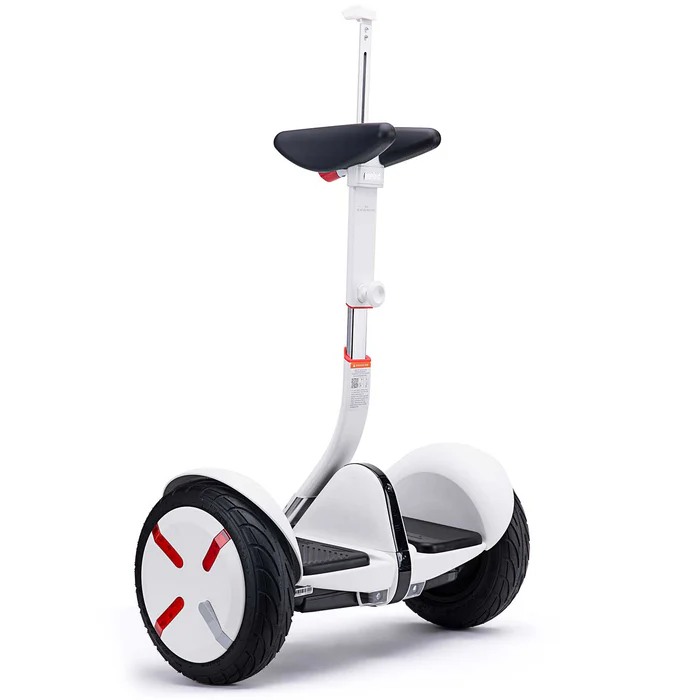
\includegraphics[width=0.5\linewidth]{Segway.png}
    \caption{Classical segway vehicle.}
    \label{fig:segway}
\end{figure}

The Segway PT's design allows for smooth and intuitive movement, controlled by shifting body weight, making it accessible to a wide range of users.

Segway vehicles have found diverse applications since their introduction. They are commonly used in urban commuting, offering a practical solution for "last-mile" travel, where public transportation might fall short. Additionally, they have become a popular choice for guided tours in cities, parks, and historical sites, providing a novel and enjoyable way to explore large areas.

In addition, Segways have been adapted for various specialized uses. In warehouses and large industrial facilities, they facilitate efficient movement of workers, enhancing productivity. Their potential extends to recreational activities and personal mobility for individuals with mobility challenges, contributing to an improvement in the quality of life.

The field of application of such vehicles is mainly circumscribed to the human-controlled side, in the sense that the rider has to change the speed, maneuver the robot with the handlebar to follow a desired trajectory, and stop.

Only in recent years the research is exploring the field of motion planning for Segway robots in order to achieve an autonomous trajectory tracking, while guaranteeing self-balancing, with the final aim of autonomous navigation.
The application area of such vehicles is wide: it can range from personal transportation of people with locomotion or visual impairments, different delivery purposes, or just simple object carrying to simplify peoples' everyday life.

The main objective of this literature review is to examine the different control techniques applied to self-balancing two-wheeled vehicles, their underlying principles, and their effectiveness.

\section{Fundamental Dynamical Properties of Segway-Like Vehicles}
\label{sec:Fundamental Dynamical Properties of Segway-Like Vehicles}

Before entering in the details of the various control methodologies, it is essential to highlight some key aspects that make the development of control algorithms for these systems particularly challenging. Understanding these fundamental points helps to explain why the study and refinement of control strategies for Segway-like vehicles have been a significant focus of research over the past 20 years an it is still ongoing.
First of all, these mechanical systems belong to the class of \textbf{Non-Linear systems}, where the laws governing the time evolution of state variables depend on their values in a manner that deviates from proportionality \cite{Khalil-2002}.
For these systems the superposition principle doesn't hold and stability analisys is much more complicated with respect to linear cases.
Moreover there are some \textit{essentially non linear phenomena} that can take place only in the presence of non linearity, among which we can mention the presence of \textbf{multiple isolated equilibria} and \textbf{limit cycles}.
Because of the powerful known tools for linear systems, the first step in analyzing a nonlinear system is usually to linearize it, but it means accepting all the limitations and approximations that derive from it.
Among this class of mechanical system, segways belongs to the subclass of underactuated mechanical systems, meaning that the number of actuators is less than the number of the system's degrees of freedom.
The study of underactuated systems has been extensively researched over the past three decades \cite{underactuated, spong2020robot}. This subclass includes significant mechanical structures such as the acrobot and the cartpole. More crucially, it encompasses all floating-base multibody systems, as discussed earlier in \cref{subsec: Floating-Base generalized coordinates}.
It is well-established \cite{Spong-underactuated} that fully actuated robots can be linearized via nonlinear feedback. Regarding underactuated robots, it is understood that the dynamic of the actuated (or active) degrees of freedom can be linearized using nonlinear feedback, while the residual dynamic following this partial linearization remain nonlinear and represent internal dynamic, requiring careful management.
The last important feature to be addressed, is something hidden inside the dynamic of the system and related to the specific configuration of the TWIP, with the body in its upright stable position:
After the linearization about that specific equilibrium, the linearized system is a \textbf{non-minimum phase system}, since the Input-Output \textit{transfer function} possesses a zero with positive real part \cite{Slotine1991AppliedNC, Hoagg-Nonminimum-phase-zeros}.
From the control perspective, performance can be limited because achieving high performance often requires high controller gains. However, high gains can lead to instability, as closed-loop poles tend to move towards open-loop zeros when the loop is closed.
The general outcome of this discussion is that controllers that imply dynamic cancellation may cancel that unstable zero with an unstable pole causing two main issues:

\begin{itemize}
    \item Any arbitrarily small discrepancy between the positive zero and the corresponding positive pole results in instability.  
    \item Even when the cancellation is perfect, an unstable controller pole cannot be used to cancel a nonminimum-phase plant zero because than that pole in closed loop is "\textit{no more a pole}", but still an eigenvalue, hiding an unstable dynamic that we are no more able to see and control \cite{Zhou1997EssentialsOR}.
\end{itemize}

All the mentioned features make TWIPs an interesting challenge from control-design perspective

\section{Review on existing control methodologies}
\label{sec:Review on existing control methodologies}

Considering all the challenges discussed thus far, this section provides an overview of the controllers that have been developed, highlighting their limitations and presenting our contributions.

We tried to categorize similar controllers, and briefly examine one by one each category.
\\

\begin{itemize}
    \item \textbf{Linear Classical and Optimal Control Methods.}  
    \item \textbf{Non-Linear Control Methods.} 
    \item \textbf{Intelligent Control Methods.} 
\end{itemize}


\subsection{Linear Classical and Optimal Control Methods}
\label{subsec:Linear Classical and Control Methods}

A common approach when dealing with a non linear system is trying to locally linearize it and exploit the various controllers known for linear systems.
Starting with model-free controllers, in \cite{Hyung-Jik-Lee} they estimated the pitch angle trough a sensor-fusion technique and then developed a single level control loop made up by a PD controller for the pendulum pitch angle and a PID controller for the position control of the system.
In \cite{Purohit2021KinematicCO} authors implemented a similar control strategy, with the difference that in this case the controller gains have been derived through a model-based approach (pole placement), starting from the linearization of the system about its unstable upright equilibrium position.
A similar approach has been followed in \cite{Johnson-et-al, Babazadeh-et-al}, comparing the results obtained with a simple PID controller, and Optimal Control theory (LQR).
The most important difference between them is that the the Optimal Control approach is based on a \textit{model} of the system, usually obtained from its equations of motion.
Then the controller gains are obtained through the minimization of a given \textit{cost functional} depending on the state-input trajectory \cite{Liberzon-calculus-of-var}.
Authors also show that LQR overperforms the simple PID, and the results improved if a precompensator is added.
The advantages of these kind of linear controllers are that they are easy to be implemented, and can work fine with a system like a TWIP because most of the time the body of the pendulum remains vertical or anyway in the neighborhood of that equilibrium, so the linearized systems behavior approximates very good the non linear one.
The drawback is that if we want to achieve higher performances in terms of accelerations and fast response, due to the system dynamic, the pitch angle has to increase accordingly, bringing the system away from its equilibrium position, making the linearized system no more reliable.
A further discussion about Optimal Control Theory is done in next chapters to highlight the main common aspects and differences with our approach.

\subsection{Non Linear Control Methods}
\label{subsec:Non Linear Control Methods}

 This review highlights the most commonly adopted non-linear control strategies for Segway control, although other approaches can be found: 

\begin{itemize}
    \item \textbf{Feedback Linearization Control (FLC)}: This is a non-linear control technique that transforms a non-linear system into an equivalent linear system through a change of variables and a nonlinear feedback control law. Essentially, it cancels out the system's non-linear dynamic, allowing linear control techniques to be applied across the entire state-space.
    It is important to note, as mentioned in the previous section, that underactuated systems cannot be fully feedback linearized \cite{Henson-et-al, Sastry1999}. Only a portion of these systems can be linearized, while the so-called internal dynamic remain non-linear. 
    This approach is known as \textbf{Partial Feedback Linearization (PFL)}. In PFL, the coordinate transformation can be complex, and ensuring the stability of the system is not always achievable.
    \\
    In \cite{Acosta-et-al} they apply PFL to the simple case of the \textit{cartpole}, while in \cite{Pathak-et-al} they do the same for the TWIP.
    In both cases they start from the dynamical model of the system obtained throguh the Newton-Euler equations, find an appropriate non-linear change of variables and derive the non-linear feedback control law; the internal dynamic stability is then guaranteed defining a proper Lyapunov Function respecting the Lyapunov second theorem for stability.
    
    \item \textbf{Model Predictive Control (MPC)} \cite{Liuping-MPC}: Model Predictive control is a control strategies involving the use of a model of the plant; the core of this algorithm is the following: knowing the new state measurement at each time step, this sample is used to solve an Optimal Control Problem with a \textit{finite time horizon}. Then only the first element of the control input trajectory is applied and this scheme is repeated at each time step.
    It is one of the most used control strategy in industry being able to handle both linear and non-linear systems with multiple control variables, and to its prediction functionality. 
    \\
    In \cite{Prabhakar-et-al} authors use MPC for the stabilization of a TWIP, developing the control algorithm in MATLAB, and testing it on a real robot; also in this case they compared the results with the one obtained through a simple PID and GA tuned PID, showing that the stabilization obtained through MPC is faster.
\end{itemize}


\subsection{Intelligent Control Methods}
\label{subsec:Intelligent Control Methods}

Intelligent controllers are advanced control systems that utilize artificial intelligence techniques, such as fuzzy logic, neural networks, and adaptive algorithms, to manage complex, nonlinear, and dynamic systems more effectively than traditional control methods. They can learn, adapt, and make decisions based on input data and environmental changes.
In many situations it is not possible to obtain precise mathematical model of the system due to its complexity and intelligent controllers can solve this problem.

\textbf{Fuzzy Logic Control}

FLC can be a MIMO system and it is based on three main steps:

\begin{itemize}
    \item Fuzzification: the process of transforming physical values to fuzzy values with the help of membership functions ranging from 0 to 1.
    \item Fuzzy Interference Process: it combines membership functions with some specific fuzzy rules, to derive the fuzzy output. 
    \item Defuzzification: it is the process that converts aggregated fuzzy sets into classical output values.
\end{itemize}
In \cite{Ahmad-et-al}, a fuzzy parallel distributed compensation (PDC) controller is introduced and implemented. They adopted the Takagi–Sugeno (TS) fuzzy model to obtain the state feedback gains required by solving the linear matrix inequalities (LMI). The results show that if strictly feasible solutions are found for the controller gains, then the fuzzy PDC controller performs better than the PID controller.
In some other approaches FL can be combined with conventional controllers obtaining a mixed control strategy: in \cite{Goher-et-al, Wu-et-al} they work on an hybrid Fuzzy/PID controller, based on the state-space model of the system, focusing on a robusteness anlisys against the model parameters.

\textbf{Neural Networks Control}

Neural networks and AI control for Segway and other two-wheeled inverted pendulum (TWIP) systems offer adaptive and robust performance by learning from data. These methods can handle complex, nonlinear dynamic and improve over time. However, they require substantial training data, computational resources, and can be challenging to interpret and debug compared to traditional control methods.
In \cite{Bature2016INTELLIGENTCF}, they explore the use of three different intelligent control methods: Fuzzy Logic Control (FLC), Neural Network Inverse Model Control (NN), and Adaptive Neuro-Fuzzy Inference System (ANFIS), for maintaining the balance and desired velocity of a two-wheeled inverted pendulum (TWIP) robot, showing that all three controllers performed well in simulations for both the tasks.
In \cite{Ahmed-et-al} it is shown an alternative control method using neural networks to replace PID controllers for controlling the cart position and handlebar angle of Segways, showing that neural network controllers are effective replacements for classical controllers, offering improved stability and performance.

Other relevant studies have been done wit intelligent controllers, all showing good results in terms of increasing performances, but with the cost of additional complexity, including dependency on the designer's expertise for fuzzy logic controllers, high energy consumption in neural network models, and the need for substantial training data.
Moreover, these methods often require significant computational resources and may not generalize well from simulations to real-world applications, posing challenges in practical deployment and tuning.

\section{Identified Challenges and Our Solutions}
\label{sec:Identified Challenges and Our Solutions}

The control of segway vehicles have been deeply explored, starting from simpler configurations like the cartpole, ending up with the final one.
Each of the previously mentioned works has its own advantages and drawbacks, and can be applied depending on the required performance.
The main outcomes regarding the actual state-of-art are the following:

Linear controllers have been the first one adopted, since they don't require the model of the system in the most of the cases, but the performances are limited by the linear approximation made for this strongly non-liner system.

Non linear model-based controllers instead have better performances with respect to the previously mentioned class, both in terms better tracking and faster stabilization. The main drawback is that they rely on the model of the system based on a reduced Lagrangian approach: starting from the conventional derivation of \textbf{EoM} the strong assumption that have been made is the no-slip constraint linking the wheels' axle center to the wheel's rotation.
This means that only one of the two variables is controlled, and if slip occurs, the controller can't do anything to correct it.

Intelligent controllers for Segway vehicles, depending on the application may not require a system model, and in general are able to achieve very good performances, with the cost of high energy consumption and significant computational resources.

For these reasons, the main contribution of this work has been the implementation of a non-linear controller (\textbf{Task Space Inverse dynamic, TSID}) where the no-slip condition is imposed as a constraint within an optimization problem.
Moreover the kinematic and dynamic model of the system have been written accordingly with the floating-base multibody convention, showing how a controller that has been in general adopted for humanoid robots, can perform effectively also with wheeled robots.

The aim of the next chapters will be that of providing a detailed description of Task Space Inverse dynamic, and how the conventional structure of the controller can be adapted to our case, in order to achieve good performance in terms of settling time and robustness with respect to model uncertainties.

\clearpage
\blankpage

\chapter{Task Space Inverse Dynamics}
\label{ch:chapter_three}%
% The \label{...}% enables to remove the small indentation that is generated, always leave the % symbol.


Task Space Inverse Dynamics (TSID) is a well known control framework in the legged robots community, popularized by Oussama Khatib \cite{Khatib1987} in 1987 and which then became a very active research topic.

The main reference for this chapter is \cite{Del-Prete2013} by Andrea Del Prete, in which can be found the detailed derivation of the control framework, and a comparison with the other most popular controllers.
In this chapter is provided the general description of TSID, focusing on the features that will then be exploited for our purpose.

As the name suggests it is important to provide a definition for the "task" and to carefully develop the robot dynamical model.
For the introduction part the robot state is called $\mathbf{x}$, while the input is called $\mathbf{u}$. 

\section{Actuation models}
\label{sec:Actuation models}

Before entering into the logic part of the controller, as in all model-based controller, it is important to choose a proper robot model, that depends not only on the robot itself, but also on the task that we would like the robot to perform, and a good starting point can be the adoption of a proper model for the actuators.
The model that we use for actuators is the \textbf{torque model}, meaning that they are assumed to be direct torque sources,but it is not the only existing one; for example as long as large contact forces are not involved, for electric motors we can assume them as direct acceleration sources.
Usually for robot that are in contact with the terrain, this is not a good assumption, since the contact forces are in the same order of magnitude of the robot's weight.
For our purposes, the best model of the actuators is to assume that they are force/torque sources.
In this case the robot state, as already written in \cref{subsec: Floating-Base generalized coordinates}, is made by its configuration $\mathbf{q}$, and its generalized velocities $\bm{\nu}$, and the control inputs are the motor torques $\bm{\tau}$.
With the assumption of the actuators as ideal torque sources, the dynamic of the robot is more complicated than a double integrator, and has the form derived in \eqref{eq: Equation of Motion}.
That form of the EoM is the classical one used in case of fully actuated systems, while for underactuated ones that equation can be decomposed into unactuated and actuated parts:

    \begin{equation}
         \begin{cases}
          M_a(\mathbf{q})\dot{\bm{\nu}} + h_a(\mathbf{q}, \bm{\nu}) = \bm{\tau} + \sum_{k \in \mathcal{I}_C} J^{T}_{a,k}\mathbf{f}_{k} 
          \\
          M_u(\mathbf{q})\dot{\bm{\nu}} + h_u(\mathbf{q}, \bm{\nu}) = \sum_{k \in \mathcal{I}_C} J^{T}_{u,k}\mathbf{f}_{k}
         \end{cases} 
         \label{eq: Equation of Motion_underactuated}
    \end{equation}

    where 
    
   \begin{equation*}
       M = \begin{bmatrix}
    M_u \\
    M_a
\end{bmatrix}, h = \begin{bmatrix}
    h_u \\
    h_a
\end{bmatrix}, J = \begin{bmatrix}
    J_u & J_a
\end{bmatrix}.
   \end{equation*}

The decoupling in \eqref{eq: Equation of Motion_underactuated} is important to show that the unactuated dynamics has only the contact forces on the right hand, and this already suggests that in order to completely control the system, we need to pay special attention to these forces.

\section{Task models}
\label{sec:Task models}

Controlling a robot means wanting it to satisfy a specific task, and after modeling the robot and its actuators, it is also necessary to develop a model for the tasks to be completed.

The \textbf{Task-Function Approach} is used, which shares some basic ideas with \textbf{Optimal Control}.
The task to be performed is described as a function that we would like to minimize.
Without loss of generality TSID assumes this function as an error between the value of a certain output function, and a reference value that we want our output to follow.
Usually the reference function is time dependent, while the output depends on both the state and the control (also on the time).
The main difference with respect to Optimal Control Theory is that in OCT the function to be minimized is a function of the state-input trajectory (usually called \textit{cost functional}), while TSID just works on the instantaneous error between the output and the reference even if both are time dependent.

\begin{table}[h]
    \centering
    \caption{TSID vs Optimal Control.}
    \label{tab:list_of_symbols}
    \renewcommand{\arraystretch}{1.5} % Increase the vertical spacing between rows
    \begin{tabular}{c c}
    \toprule
    \textbf{Approach} & \textbf{Cost Function} \\
    \midrule
    TSID & $e(x,u,t) = y(x,u) -y^{n}(t) $\\
    \hline
    Optimal Control & $ J = \int_{t_0}^{t_f} s(x(t), u(t), t) \, dt $\\
    \bottomrule
    \end{tabular}
\end{table}

There can be different types of task functions, but for the development of the E-Cargo controller the main interest is related to linear functions of the the control input \textbf{u}, and \textbf{non linear functions of robot configuration} such that:

    \begin{equation}
         e(\mathbf{q},t) = y(\mathbf{q}) - y^{n}(t).
         \label{eq: Task function}
    \end{equation}

Something that requires more attention, is that what we can instantaneously control and select the control input \textbf{u}, but not directly the state, since only the state derivative is affected by the control input.
In particular in our purpose we can instantaneously change the robot accelerations since the actuators have been modeled as torque sources, meaning that we can't directly satisfy the task function in \eqref{eq: Task function}.

To overcome this issue a dynamics of the task function is imposed, affecting the derivatives of this function $e(\mathbf{q},t)$ in a way that $\lim_{t \to \infty} e(\mathbf{q},t) = 0$, since that one is the minimum that we would like to achieve to have the output exactly following the reference.

We want to end up in an affine function of the robot generalized acceleration $\dot{\bm{\nu}}$ (the fact that it is affine is important for computational aspects).

Starting from \eqref{eq: Task function}, we can impose a second order linear error dynamic (we could also impose a non linear dynamic to the task function, but a linear dynamic is enough in most of the cases).:

\begin{equation*}
    \ddot{e} = -K_d\dot{e} -K_pe.
\end{equation*}

This obtained linear dynamical system is stable if both $K_p$ and $K_d$ are positive.

Expanding the term $e(\mathbf{q},t)$, the previous equation becomes

\begin{equation}
    \ddot{y} - \ddot{y}^{n}  = -K_d(\dot{y}-\dot{y}^{n}) -K_p(y - y^{n}).
    \label{eq: Task dynamics}
\end{equation}

Then some of the terms involved in Equation \eqref{eq: Task dynamics} are grouped together in a single one that we call \textbf{desired acceleration}

\begin{equation}
    \ddot{y}^{*} = \ddot{y}^{n} -K_d(\dot{y}-\dot{y}^{n}) -K_p(y - y^{n}).
    \label{eq: Desired Acceleration}
\end{equation}

The core of this approach is to try to express the second output derivative $\ddot{y}$ as a function of the robot generalized acceleration $\dot{\bm{\nu}}$, and so the first output derivative $\dot{y}$ as a function of the robot generalized velocity $\bm{\nu}$.
Then it will be seen that is important to obtain functions that are \textbf{affine} in the sense that \cite{boyd2004convex}, given $f: \mathbb{R}^n \to \mathbb{R}^m$, $f$ can be expressed as:

\begin{equation*}
    f(\mathbf{x}) = A\mathbf{x} + \mathbf{b},
\end{equation*}

where: $\mathbf{x} \in \mathbb{R}^n$ is the input vector, $\mathbf{A} \in \mathbb{R}^{m \times n}$ is a matrix representing the linear transformation, $\mathbf{b} \in \mathbb{R}^m$ is a vector representing the translation.

According to this definition, Equation \eqref{eq: Task dynamics} has to be written as:

\begin{equation*}
        J_{T}\dot{\bm{\nu}} + \dot{J_{T}}\bm{\nu} - \ddot{y}^{n} = -K_d(\dot{y}-\dot{y}^{n}) -K_p(y - y^{n}) ,
\end{equation*}

and so:

\begin{equation}
        J_{T}\dot{\bm{\nu}} = \ddot{y}^{n} - \dot{J_{T}}\bm{\nu} - K_d(\dot{y}-\dot{y}^{n}) - K_p(y - y^{n}).
        \label{eq: Task equation with Jacobians}
\end{equation}

Equation \eqref{eq: Task equation with Jacobians} shows that the affine function is obtained through the Jacobian that has been called $J_{T}$ meaning for \textbf{Task Jacobian} and represents the derivatives of the output with respect to the base generalized velocity: $J_{T} = \frac{\partial y}{\partial \bm{\nu}}$.

What we have in the end is an affine function of the robot acceleration and control input, as:

\begin{equation}
        \mathbf{g}(\mathbf{v}) = \begin{bmatrix}
            A_{\nu} & A_{u}
        \end{bmatrix} \begin{Bmatrix}
            \bm{\dot{\nu}} \\
            \mathbf{u}
        \end{Bmatrix}.
        \label{eq: Affine preliminar function}
\end{equation}

In next equations the matrix $\begin{bmatrix}
            A_{\nu} & A_{u}
        \end{bmatrix}$ id called 'A' , and  $\begin{Bmatrix}
            \bm{\dot{\nu}} \\
            \mathbf{u}
        \end{Bmatrix}$ is called $\mathbf{v}$

\section{Optimization Problem Formulation}
\label{sec:Optimization Problem Formulation}

The task definition, along with the robot control model, has been carefully designed to be the foundation of an \textbf{optimization-based control} method.
As previously mentioned, the idea of formulating control problems like optimization problems, follows from OCT.
The key elements are:

\begin{itemize}
    \item \textbf{robot state}: $\mathbf{x} = (\mathbf{q},\bm{\nu})$
    \item \textbf{control input}: $\mathbf{u} = \bm{\tau}$
    \item \textbf{robot dynamic model}: $ M(\mathbf{q})\dot{\bm{\nu}} + C(\mathbf{q},\bm{\nu})\bm{\nu} + \mathbf{g}(\mathbf{q}) = S\bm{\tau} + \sum_{k \in \mathcal{I}_C} J^{T}_{k}\mathbf{f}_{k}$
    \item \textbf{task function to minimize}: $\|\mathbf{g}(\mathbf{v})\|_2 = \| A\mathbf{v} - \mathbf{a}\|_2$
\end{itemize}

Notice that the task function in Equation \eqref{eq: Affine preliminar function} is a vector valued function, but from an optimization point of view, the concept of minimizing a vector is meaningless; for this reason what is actually minimized is $\|\mathbf{g}(\mathbf{v})\|_2$ which is a quadratic function.

The final step in setting up the optimization-based control is to introduce and appropriately model the necessary constraints.

\subsection{Constraints model}
\label{subsec:Constraints model}

The role of the contact forces has been already mentioned at the beginning of this chapter, but requires a more accurate analysis:
we have seen in Equation \eqref{eq: Equation of Motion_underactuated} how they drive the unactuated robot dynamics, in all cases in which the robot is in contact with the external environment.
There are two main ways to model contacts between mechanical systems and the environment:

\begin{itemize}
    \item \textbf{Soft Contact Models} that do not constrain the motion;
    \item \textbf{Rigid Contact Models} that constrain the motion.
\end{itemize}

We use the Rigid Contact Model because it provides a more reasonable approximation for our purposes. This model imposes constraints on motion: once the robot is in contact with the ground, it cannot move downwards or penetrate the ground.

TSID models constraints in the same way of tasks; we can start from a non linear function of the robot configuration

\begin{equation}
    c(\mathbf{q}) = 0
    \label{eq: contact point general constraint}
\end{equation}

enforcing that the points of the robot that are in rigid contact with the environment don't move; the strong assumption behind this formulation is that if the robot is in contact, it can't break the contact (because the contact point could move in some directions, but here all its possible motions are constrained).
The main outcome of this assumption is that we have to know if the robot is in contact or not with the ground, in order to activate/deactivate the constraint. 
What stated is reasonable for legged robot, and will be adapted to the case of the TWIP in next chapters.

Starting from Equation \eqref{eq: contact point general constraint}, we will incorporate this as a constraint in our QP by following the same procedure used for the task definition, knowing that we can't directly impose a function of the robot configuration, but deriving it twice, we can impose an affine function of the robot generalized acceleration (constraining the contact points accelerations to be null):

\begin{equation}
    {J_{R}}\dot{\bm{\nu}} + \dot{J}_{R}\bm{\nu} = 0
    \label{eq: Contact dynamics with Jacobians}
\end{equation}

where ${J_{R}}$ represents the derivatives of the output chosen to describe the contact with respect to the base generalized velocity ${J_{R}} = \frac{\partial c}{\partial \bm{\nu}}$. 

By imposing Equation \eqref{eq: Contact dynamics with Jacobians} we are ensuring also Equation \eqref{eq: contact point general constraint} given the implicit initial conditions of "being in contact".

\subsection{TSID Problem Statement}
\label{subsec:TSID Problem Statement}

At this stage, we can outline the basic framework of our optimization problem aimed at minimizing the task functions by determining optimal control inputs, considering both the EoM and the contact model as equality constraints:

\begin{center}
$\underset{\bm{\dot{\nu},f_{c},\bm{\tau}}}{\text{argmin}} \| A\mathbf{v} - \mathbf{a}\|^{2}$

\text{subject to}

\end{center}

\begin{equation}
\begin{bmatrix} 
M & -J_{c}^{T} & -S^{T}  \\
J_{R} & 0 & 0  \\
\end{bmatrix} 
\begin{Bmatrix} 
\bm{\dot{\nu}} \\
\mathbf{f_{c}} \\
\bm{\tau}  \\
\end{Bmatrix} 
= 
\begin{Bmatrix} 
-\mathbf{h} \\
-\dot{J}_{R} \\
\end{Bmatrix}
\label{eq: first QP-setup}
\end{equation}

In \eqref{eq: first QP-setup}, $\mathbf{v}$ is the vector of the optimization variables containing the robot generalized acceleration $\bm{\dot{\nu}}$, the torques vector $\bm{\tau}$, and the contact forces $\mathbf{f_{c}}$.
What can be demonstrated, and has been done in \cite{Mistry-et-al, Park_Khatib_2008} is that in the case of rigid contacts, contact forces are a direct function of the joint torques, so by selecting the joint torques the solver can indirectly select the contact forces: this explains why we are able to add contact forces to the vector of optimization variables.
The cost function is a convex quadratic function of the optimization variables and, since the constraints are affine, this problem is a \textbf{Convex Quadratic Program (QP)}.

To be more precise about the definitions, the cost function is the square of an affine function of the optimization variables, and so a special kind of convex quadratic function, so the problem is a \textbf{Least-Squares Problem (LSP)}.

Throughout this work we will just refer to it as a generic QP.

So far this control problem can be classified as an \textbf{Equality-Constrained Least-Squares Problem (ECLSP)}.
It is well known that uncostrained LSP, can be solved through \textbf{pseudo-inverse}, meaning that the solution of: 
\begin{equation*}
    \underset{\mathbf{v}}{\text{argmin}} \| A\mathbf{v} - \mathbf{a}\|^{2}
\end{equation*}
is directly given by:
\begin{equation*}
    \mathbf{v}^{*} = A^\dagger \mathbf{a}
\end{equation*}

When only equality constraints are added, the pseudo-inverse solution still holds, and so the solution of a problem like:

\begin{center}
\begin{equation*}
    \underset{\mathbf{v}}{\text{argmin}} \| A\mathbf{v} - \mathbf{a}\|^{2}
\end{equation*}
\text{subject to;}
\begin{equation*}
    B\mathbf{v} = \mathbf{b}
\end{equation*}

\end{center}

is directly given by:
\begin{equation*}
    \mathbf{v}^{*} = B^{\dagger}\mathbf{b} + N_B (AN_B)^{\dagger}(\mathbf{a} - AB^{\dagger}\mathbf{b})
\end{equation*}

where $N_B = I - B^{\dagger}B$ is the null-space projector of $B$.

Everything changes when \textbf{inequality constraints} are added, because in these cases the optimization problem can no more be solved through pseudo-inverses, and this is why the QP formulation has been introduced.

The most common inequality constraints that are used in robotics are the following affine functions of optimization variables $\mathbf{v}$:

\begin{itemize}
    \item Joint torque bounds: $\tau_{\min} \leq \tau \leq \tau_{\max}$.
    \item Linear approximation of force friction cones: $B\mathbf{f_c} \leq 0$.
    \item any other equality-like constraint expressed with a slack variable: $d\mathbf{v} + \xi = 0$.
\end{itemize}

We will show how to deal with them for our specific purpose.

\subsection{Multi-Task Optimization}
\label{subsec:Multi-Task Optimization}

So far we have described the basic idea of the TSID controller, when the task model has been formulated for just one task; in most of the cases this is not enough since we want the robot to perform multiple tasks, for example follow a trajectory, while keeping a balancing of its center of mass.
Some of these tasks can have more priority with respect to the others (usually the balancing task is more important then the tracking one), and this problem can be tackled in different ways.
Here we are going to describe the simpler idea, which is the one used in our developments, and is called \textbf{Weighted Multi-Objective Optimization}.

Assuming that the robot has to perform $N$ tasks, each defined by a proper task function

$$
\|\mathbf{g_{i}}(\mathbf{v})\|^{2} = \| A_{i}\mathbf{v} - \mathbf{a_{i}}\|^{2} \quad \text{for} \quad i = 1, \ldots, N
$$

this approach prescribes to sum all these functions, each multiplied by a proper user-defined \textbf{weight} $w_{i}$; in this way the control problem can be rewritten as:

\begin{center}
$\underset{\bm{\dot{\nu},f_{c},\bm{\tau}}}{\text{argmin}} \| \sum_{i=1}^{N} w_i \mathbf{g}_{i}(\mathbf{v}) \|^{2}$

\text{subject to}

\end{center}

\begin{equation}
\begin{bmatrix} 
M & -J_{c}^{T} & -S^{T}  \\
J_{R} & 0 & 0  \\
\end{bmatrix} 
\begin{Bmatrix} 
\bm{\dot{\nu}} \\
\mathbf{f_{c}} \\
\bm{\tau}  \\
\end{Bmatrix} 
= 
\begin{Bmatrix} 
-\mathbf{h} \\
-\dot{J}_{R} \\
\end{Bmatrix}
\label{eq: First Multi-task QP-setup}
\end{equation}

The higher the weight $w_{i}$, the more important the corresponding task $\mathbf{g}_{i}(\mathbf{v})$ is. 

Given that the sum of least-squares function is still a least-squares function, the problem remains a LSP.
A possible weak point of this approach is that finding weights can be difficult, and if the tasks are many, each one more important than the other, it can happen to end up with too large/small weights leading to numerical issues.

To solve the mentioned issues, a different a more complicated 
approach can be used, called \textbf{Hierarchical Multi-Objective Optimization}, where the key idea is to order the task functions, according to \textbf{priorities} \cite{Romano2015WholebodyFC}\cite{Escande2014HierarchicalQP}.



\part{Contributions}\label{part:Contributions}

\chapter{Controller Theory}
\label{ch:chapter_four}%
% The \label{...}% enables to remove the small indentation that is generated, always leave the % symbol.

\section{E-Cargo System}
\label{sec:E-Cargo}

As introduced in the first chapters, the object of this thesis is a Smart Electric Cargo (Figure \ref{fig:E-Cargo CAD drawing}).


\begin{figure}
    \centering
    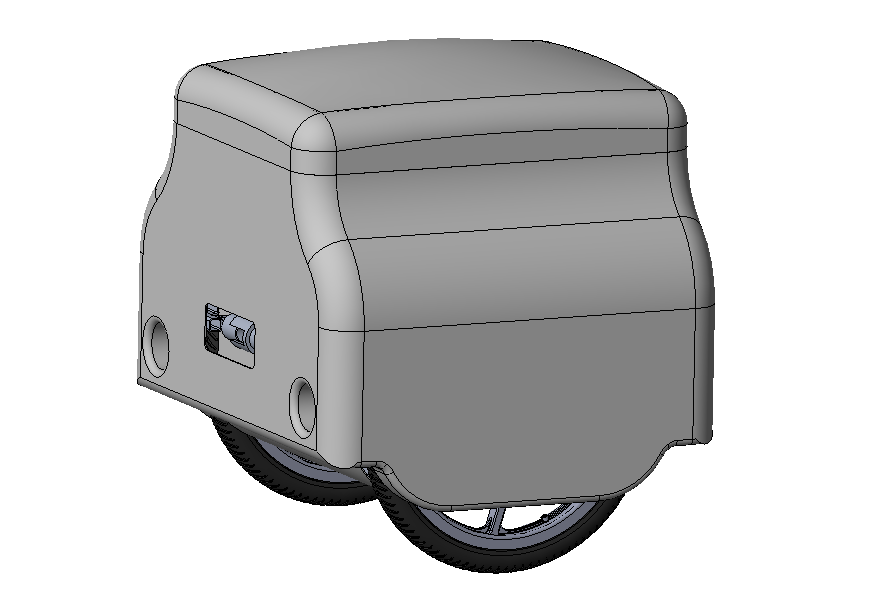
\includegraphics[width=0.5\linewidth]{e-Cargo CAD.png}
    \caption{E-Cargo CAD drawing.}
    \label{fig:E-Cargo CAD drawing}
\end{figure}

The mechanical design has been realized, taking into account that the Center of Mass must always lye above the wheels' axle and so all the electronic devices (sensors, computers, battery...) are placed accordingly.
This design makes the E-Cargo a TWIP also for the unloaded configuration.

The motion is given by two in-wheeled electric motors (BLDC), and two small safety wheels (not represented in the CAD) have been mounted on both sides to guarantee an initial starting pitch angle of $\approx 25^{\circ}$.
Table \ref{tab:E-Cargo Mechanical Parameters} provides a summary of all the key parameters relevant to the controller simulation, which can help in better understanding the results.
The numbers are qualitative since the mechanical/design concept is still evolving:

\begin{table}[H]
    \centering
    \renewcommand{\arraystretch}{1.5} % Increase the vertical spacing between rows
    \begin{tabular}{@{}l@{\hspace{1.5cm}}l@{\hspace{1.5cm}}l@{\hspace{1.5cm}}l@{\hspace{1.5cm}}l@{}}
    \toprule
    \textbf{Symbol} & \textbf{Description} & \textbf{Units} & \textbf{Value} & \textbf{Notes} \\
    \midrule
    $m$ & Mass of the cargo & $kg$ & 20 & mass unloaded \\
    $m_{p}$ & Mass of payload & $kg$ & 40 & maximum payload \\
    $I_y$ & Y Moment of inertia & $kg m^2$ & 3.3 & pitch moment of Inertia  \\
    $I_z$ & Z Moment of inertia & $kg m^2$ & 2.4 & yaw moment of inertia \\
    $r_w$ & Wheel radius & $m$ & 0.2 & wheel radius \\
    $CoM_{z}$ & CoM height & $m$ & 0.3 & Max CoM height w.r.t wheels' axle \\
    $b$ & axle length & $m$ & 0.6 & length of the wheels' axle \\
    $h$ & height & $m$ & 0.9 & total height \\
    $l$ & length & $m$ & 0.5 & total length \\
    $w$ & width & $m$ & 0.6 & total width \\
    \bottomrule
    \end{tabular}
    \caption{E-Cargo Mechanical Parameters.}
    \label{tab:E-Cargo Mechanical Parameters}
\end{table}


\section{E-Cargo Dynamical Model}
\label{sec:E-Cargo Dynamical model}

In \cref{ch:chapter_three} we have described the basic architecture of the control framework; in this chapter, we will follow the same approach, adapting each case specifically to our robot.
Starting from the EoM written for a generic floating base system:

    \begin{equation*}
          M(\mathbf{q})\dot{\bm{\nu}} + C(\mathbf{q},\bm{\nu})\bm{\nu} + \mathbf{g}(\mathbf{q}) = S\bm{\tau} + \sum_{k \in \mathcal{I}_C} J^{T}_{k}\mathbf{f}_{k},
    \end{equation*}

there are two main aspects that require more details:

    \begin{itemize}
        \item The Contact wrench $\mathbf{f}_{k}$.
        \item The Contact Jacobian $J_{k}$.
    \end{itemize}

\subsection{Contact Wrench}
\label{subsec:Contact Wrench}

A first definition for the contact wrench representing the total forces acting on a rigid body has been provided in \cref{sec:Force-Torque covectors}.
It has been described as a vector 

\begin{equation}
    {}_{B}\mathbf{f} = 
    \begin{Bmatrix}
    {}_{B}\bm{f} \\
    {}_{B}\bm{\mu}
    \end{Bmatrix} \in \mathbb{R}^{6}
\end{equation}

with dimension 6.
The actual dimension of the wrench depends on the assumption that we make on the "\textit{dimension}" of the contact.
For legged robots, the contact is usually assumed to be a surface (the bottom surface of the foot); a force reduction is performed to end up with a point contact, and if this point is a generic one on the surface, this reduction leads to 3 linear components (forces) and 3 angular components (moments)(Figure\ref{fig:6DContact_Wrench}).


\begin{figure}
    \centering
    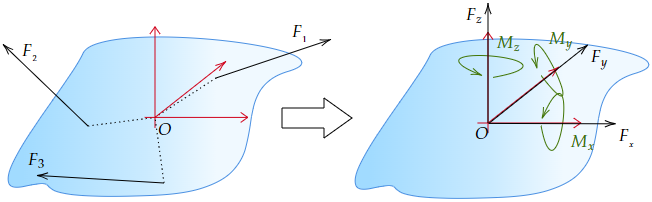
\includegraphics[width=0.65\linewidth]{6DContact_Wrench.png}
    \caption{6D Contact Wrench.}
    \label{fig:6DContact_Wrench}
\end{figure}

In our study, we opted for the following contact modeling assumptions:

\begin{itemize}
    \item Rigid contact model;
    \item Wheels modeled as unidimensional disks;
\end{itemize}

\begin{figure}[H]
    \centering
    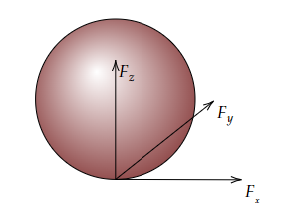
\includegraphics[width=0.35\linewidth]{3DContact_Wrench.png}
    \caption{3D Contact Wrench.}
    \label{fig:3DContact_Wrench}
\end{figure}

These two assumptions result in a final 3D contact wrench, as illustrated in Figure \ref{fig:3DContact_Wrench}. This follows from the fact that the rigid contact between a disk and a plane is inherently a point contact defined by the nature of the interaction and not resulting from a reduction of forces; this is the reason why the angular components are not involved.
The wrench becomes defined as

\begin{equation}
    {}_{B}\mathbf{f} = 
    \begin{Bmatrix}
    {}_{B}\bm{f} \\
    \end{Bmatrix} = 
    \begin{Bmatrix}
    {}_{B}{f}_{x} \\
    {}_{B}{f}_{y} \\
    {}_{B}{f}_{z} 
    \end{Bmatrix} \in \mathbb{R}^{3}.
    \label{eq:3DContact_Wrench}
\end{equation}

Considering that there are two wheels, the total number of contact forces involved is six. The combined contact wrench, derived from the stacking of the two individual wrenches, will be defined as follows:

\begin{equation}
    {}_{B}\mathbf{f}= \sum_{k \in \mathcal{I}_C} {}_{B}\mathbf{f}_{k} = \begin{Bmatrix}
    {}_{B}\bm{f}_l \\
    {}_{B}\bm{f}_r
    \end{Bmatrix} \in \mathbb{R}^{6},
    \label{eq:Total Contact Wrench}
\end{equation}

where ${}_{B}\bm{f}_l$ denotes the contact wrench that acts on the left wheel and ${}_{B}\bm{f}_r$ denotes the contact wrench acting on the right wheel.

\subsection{Rolling Contact Jacobian}
\label{subsec:Rolling Contact Jacobian}

The concept of the contact Jacobian has been introduced in \cref{subsec: Geometric Jacobians}, together with the most complete notation
    \begin{equation*}
        {}^{C_i} J_{A,L/X}(\mathbf{q}) = {}^{C_i}X_{L} {}^{L}J_{A,L/X}(\mathbf{q}).
    \end{equation*}
With reference to Equation \eqref{eq: General contact Jacobian} what has to be higlighted is that, considering a generic link $L$, experiencing the contact $C_i$, in general:
$${}^{C_i} J_{A,L/X}(\mathbf{q}) \neq {}^{C_i}J_{A,C_i/X}(\mathbf{q}),$$
because the frame $C_i$ that is experiencing the contact at a given time instant, can move with respect to the link $L$ and this exactly what happens in the case of a rolling contact.

\begin{figure}
    \centering
    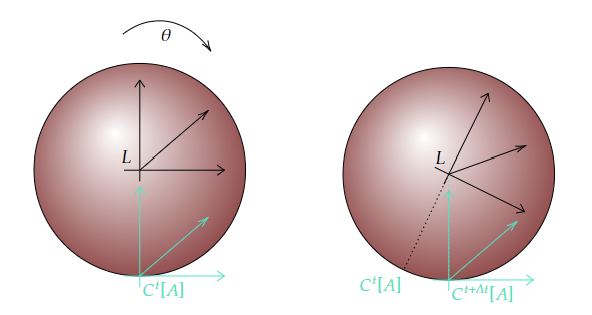
\includegraphics[width=0.5\linewidth]{Rolling_Contact.png}
    \caption{Rolling contact.}
    \label{fig:Rolling contact}
\end{figure}


So in simple words what is usually done is computing the Jacobian of the link's reference frame, and then shifting it to the contact point through a properly defined transformation $X$.


Since we decided to express all in \textit{mixed} representation, the contact Jacobian can be defined as:

    \begin{equation}
        {}^{C_i[A]} J_{A,L/B[A]}(\mathbf{q}) = {}^{C_i[A]}X_{L[A]} {}^{L[A]}J_{A,L/B[A]}(\mathbf{q}),
    \end{equation}
    
where ${}^{L[A]}J_{A,L/B[A]}$ is the \textit{doubly mixed} Jacobian of the wheel calculated in its CoM, and ${}^{C_i[A]}X_{L[A]}$ is a matrix defined as:

\begin{equation}
{}^{C[A]}  X_{L[A]} = \begin{bmatrix} 
{}^{C[A]}  R_{[A]} &    {}^{C[A]} o^\wedge_{L[A]}  {}^{C[A]} R_{L[A]} \\
0_{3x3} & {}^{C[A]} R_{L[A]}\\  
\end{bmatrix}
\end{equation}

that for this specific application, and considering the terrain flat, is just:

\begin{equation}
{}^{C[A]}  X_{L[A]} = \begin{bmatrix} 
I_{3 \times 3} &    {}^{C[A]} o^\wedge_{L[A]} I_{3 \times 3} \\
0_{3x3} & I_{3 \times 3}\\  
\end{bmatrix}.
\end{equation}

Equation \eqref{eq:doubly mixed Jacobian definition} allows us to compute the contact forces even if the contact point changes due to the rolling motion.

From now on, to simplify the notation we will denote ${}^{C_i[A]} J_{A,L/B[A]}(\mathbf{q})$ as $J_{C_{L}}$ for the left wheel and $J_{C_{R}}$ for the right wheel.

For a more compact notation we can stack the Jacobians together (as we did for the wrenches) obtaining the \textbf{overall contact Jacobian} defined as

\begin{equation}
    J_{C} = \begin{bmatrix}
    S_{J_{C}}J_{C_{L}} \\
    S_{J_{C}}J_{C_{R}}
\end{bmatrix} \in \mathbb{R}^{6 \times 8},
\label{eq:overall contact Jacobian}
\end{equation}

where $S_{J_{C}}$ is a selection matrix defined as

\begin{equation}
    S_{J_{C}} = \begin{bmatrix}
        1 & 0 & 0 & 0 & 0 & 0 \\
        0 & 1 & 0 & 0 & 0 & 0 \\
        0 & 0 & 1 & 0 & 0 & 0 \\
    \end{bmatrix}.
\end{equation}

Considering that the input vector $\bm{\tau}$ contains the two torques acting on the left and on the right wheel, respectively, as

\begin{equation}
    \bm{\tau} = \begin{Bmatrix}
    \tau_{L} \\
    \tau_{R}    
\end{Bmatrix} \in \mathbb{R}^{2}.
\end{equation}

The final expression of the robot dynamic equation is given as

\begin{equation}
      M(\mathbf{q})\dot{\bm{\nu}} + C(\mathbf{q},\bm{\nu})\bm{\nu} + \mathbf{g}(\mathbf{q}) = S\bm{\tau} + J_{C} {}_{B}\mathbf{f}.
      \label{eq:e-Cargo dynamic equation}
\end{equation}

\section{Tasks definition}
\label{sec:Tasks definition}

The task definition depends on the specific actions that we want our robot to perform.
In our case, the concept is still evolving, but generally, it requires autonomous navigation and self-balancing:

\begin{itemize}
    \item By \textbf{self-balancing}, we mean that the E-Cargo, given is TWIP configuration, must not fall down.
    \item By \textbf{Tracking}, we mean that the E-Cargo must be able to follow a person or a given signal, requiring as a consequence a control in position.
\end{itemize}

In \cref{ch:chapter_three} we have seen how tasks and constraints have a similar formulation, and this allows to interchange them when needed.

As a starting point we consider them both as tasks, and we will see how to deal with both, starting from the first one.

From this section on, the part of the E-Cargo including the body and payload (i.e., everything above the wheels' axle) is referred to as the "upper assembly" and will be modeled as a single rigid body called \textit{base} $B$.

\subsection{Self-Balancing Task}
\label{subsec:Self-Balancing Task}

The Self-Balancing is the robot's most important feature because, without it, none of the other tasks can be reliably performed.

\begin{figure}
    \centering
    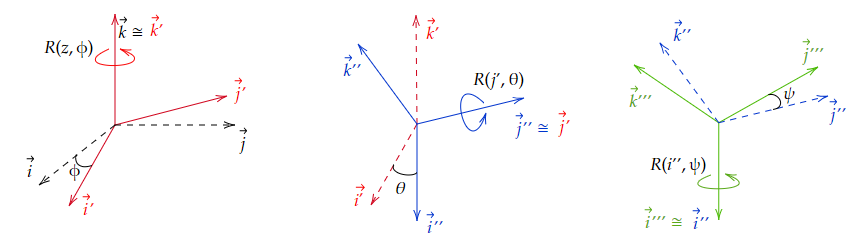
\includegraphics[width=0.9\linewidth]{RPY.png}
    \caption{Yaw-Roll-Pitch decomposition.}
    \label{fig:Yaw-Roll-Pitch decomposition}
\end{figure}

To ensure this, according to Figure \ref{fig:Yaw-Roll-Pitch decomposition} we choose to control the pitch angle of the body named $\theta$.

In the body reference frame, the base angular velocity ${}^{B} \omega_{A,B}$ can be obtained as

\begin{equation}
    {}^{B} \bm{\omega}_{A,B} = \dot{\phi}\,{}^{B}\vec{k} + \dot{\theta}\,{}^{B}\vec{j}' + \dot{\psi}\,{}^{B}\vec{i}''.
    \label{eq:Base_ang_Vel}
\end{equation}

We want to pass to the mixed representation in which we need the right-trivialized base angular velocity ${}^{A} \bm{\omega}_{A,B}$, and to do so we project the geometric vectors involved, in the proper inertial frame defined by:

\begin{equation*}
    {}^{A}\vec{i} = \begin{Bmatrix}
        1 \\
        0 \\
        0
    \end{Bmatrix} ;     {}^{A}\vec{j} = \begin{Bmatrix}
        0 \\
        1 \\
        0
    \end{Bmatrix} ; {}^{A}\vec{k} = \begin{Bmatrix}
        0 \\
        0 \\
        1
    \end{Bmatrix};
\end{equation*}

meaning that 

\begin{equation}
    \begin{cases}
        {}^{B}\vec{j}' = R_z(\phi)\,{}^{A}\vec{j} \\
        {}^{B}\vec{i}'' = R_y(\theta)\,{}^{A}\vec{i}' = R_y(\theta) \cdot R_z(\phi)\,{}^{A}\vec{i} \\
        {}^{B}\vec{k} = {}^{A}\vec{k}
    \end{cases}
    \label{eq:inertial_geometric_projection}
\end{equation}

where $R_z(\phi), R_y(\theta)$ are the matrices describing the elementary rotations.

Putting together Equation \eqref{eq:Base_ang_Vel} and Equation \eqref{eq:inertial_geometric_projection} we obtain

\begin{equation}
    {}^{A} \bm{\omega}_{A,B} = {}^{A}J_{YRP} \begin{Bmatrix}
        \dot{\psi} \\
        \dot{\theta} \\
        \dot{\phi} 
    \end{Bmatrix}
    \label{eq:from YRP vel to base ang vel}
\end{equation}

where 

\begin{equation}
    {}^{A}J_{YRP} = \begin{bmatrix}
        R_y(\theta) \cdot R_z(\phi)\,{}^{A}|\vec{i}| & R_z(\phi)\,{}^{A}|\vec{j}| & {}^{A}|\vec{k}|
    \end{bmatrix}.
    \label{eq:YRP Jacobian}
\end{equation}

Our intent is to express the pitch angle $\theta$ as a function of the robot's configuration, and therefore its angular velocity and acceleration as a function of the robot's generalized velocity and acceleration; this just requires the inverse of ${}^{A}J_{YRP}$ and its derivative in such a way that

\begin{equation}
\begin{Bmatrix}
        \dot{\psi} \\
        \dot{\theta} \\
        \dot{\phi} 
    \end{Bmatrix} = {}^{A}J^{-1}_{YRP} {}^{A} \bm{\omega}_{A,B}
    \label{eq: YRP velocities},
\end{equation}

and more important

\begin{equation}
    \begin{Bmatrix}
        \ddot{\psi} \\
        \ddot{\theta} \\
        \ddot{\phi} 
    \end{Bmatrix} = {}^{A}\dot{J}^{-1}_{YRP} {}^{A} \bm{\omega}_{A,B} + {}^{A}J^{-1}_{YRP} {}^{A} \bm{\dot{\omega}}_{A,B}.
    \label{eq: YRP accelerations}
\end{equation}

The expression used inside the controller in the end is

\begin{equation}
    \ddot{\theta} = S_{\theta}{}^{A}J^{-1}_{YRP}S_{\omega}J_{B}\dot{\bm{\nu}} - S_{\theta}{}^{A}\dot{J}^{-1}_{YRP}S_{\omega}J_{B}\bm{\nu}
    \label{eq: Pitch angular acceleration}.
\end{equation}

The complete derivation of the equation can be found in the \cref{ch:Appendix}, here is just reported the final formulation of the pitch angular acceleration as a function of the robot'sgeneralized acceleration.

The last passage is to define the error function to be minimized by the controller as stated in Equation \eqref{eq: Task equation with Jacobians}.

That passage is solved with a simple manipulation of Equation \eqref{eq: Pitch angular acceleration}
defining the task Jacobian as

\begin{equation}
    J_{T_P} = S_{\theta}{}^{A}J^{-1}_{YRP}S_{\omega}J_{B},
    \label{eq: Pitch Task Jacobian}
\end{equation}

such that 

\begin{equation*}
     \ddot{\theta} = J_{T_P}{\dot{\bm{\nu}}} - \dot{J}_{T_P}\bm{\nu}.
\end{equation*}

Adopting the definition of desired acceleration provided in Equation \eqref{eq: Desired Acceleration}

\begin{equation}
    \ddot{\theta}^{*} = \ddot{\theta}^{n} -K_{d\theta}(\dot{\theta}-\dot{\theta}^{n}) -K_{p\theta}(\theta - \theta^{n}).
    \label{eq: Pitch Desired Acceleration}
\end{equation}

The final error function used for pitch control inside the TSID is 

\begin{equation}
   e(\theta,t) = J_{T_P}{\dot{\bm{\nu}}} - \dot{J}_{T_P}\bm{\nu} - \ddot{\theta}^{*}. 
    \label{eq: Pitch error task}
\end{equation}

\subsection{Tracking Task}
\label{subsec:Tracking Task}

The starting point for setting up the tracking problem is defining "what" we want to control to ensure the following of a given trajectory.
We decided to control a $point$ to which we want to impose generic nominal trajectories, which will be defined later on.
One thing that can be realized at this point is that we can't directly control the base reference frame $B$ due to a robot kinematic singularity.

In fact, if we see the trailer from the top (x-y) plane it can be seen as a unicycle \cite{ZHOU202354}, which instantaneously cannot have velocity components aligned with $\vec{y_B}$;
If we consider a point $\mathbf{P}$ coincident with the origin of the base reference frame $B$, which we assume in the middle of the wheels' axle, its instantaneous velocity is expressed as:

$$ \dot{\mathbf{P}} = v \vec{\bm{x_B}},$$

$$ \begin{Bmatrix}
\dot{P_x} \\
\dot{P_y}
\end{Bmatrix} = v \begin{Bmatrix}
\cos\gamma \\
\sin\gamma
\end{Bmatrix},
$$

ended up in an underactuated system.

\begin{figure}
    \centering
    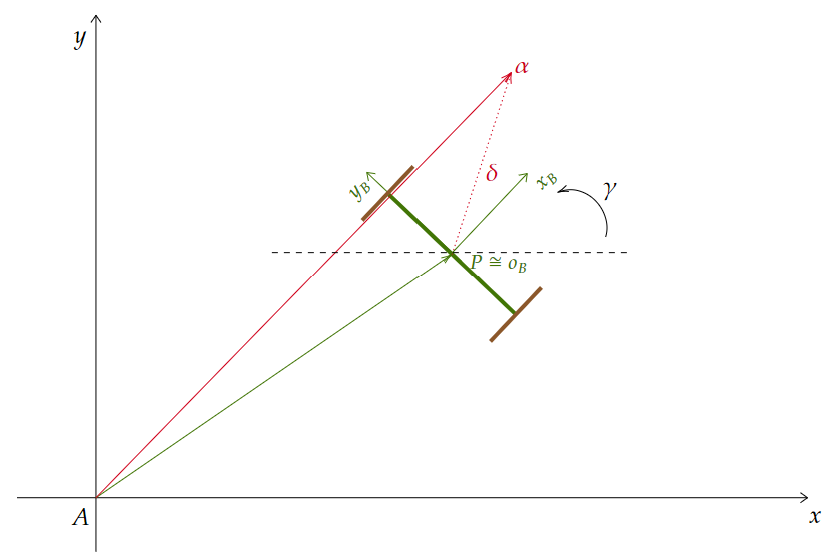
\includegraphics[width=0.7\linewidth]{unicycle singularity.png}
    \caption{Unicycle singularity.}
    \label{fig:Unicycle singularity}
\end{figure}


To address this undesirable behavior, our solution has been as follows: instead of controlling $P_x , P_y$, we control the $x-y$ position of a point ($\bm{\alpha}$) which is rigidly attached to the base, at a distance $\bm{\delta}$ from it, as shown in the image above. 

If we call A the world frame, the following relations can be written:

\begin{equation}
{}^{A} \bm{\alpha} = {}^{A}\mathbf{P} + {}^{A} R_{B} {}^{B} \bm{\delta}.
\label{eq:control point generic}
\end{equation}

This solution is enough for which concerns the tracking itself, but there is still something hidden in the robot dynamics, that makes the whole control problem unfeasible: when switching to the accelerations level (but this can also be directly observed from the position), the acceleration of this point becomes instantaneously linked to the pitch angular acceleration, making their coupled control complex.

This has been the reason why we kinematically defined a point which is still rigidly connected with the base reference frame $B$, but doesn't rotate with the base around the axis $y_B$ as described in Figure \ref{fig:accelerations decoupling}.
What changes between the two definitions is just the matrix ${}^{A}R_{B}$ which is no more the rotation matrix between frames $B$ and $A$, but become the matrix describing the \textit{elementary rotation} around the axis $z$, and we will call it ${}^{A}R^{xy}_{B}$

\begin{equation}
{}^{A} R_B^{xy} = \begin{bmatrix}
\cos(\psi) & -\sin(\psi) & 0 \\
\sin(\psi) & \cos(\psi) & 0 \\
0 & 0 & 1 \\
\end{bmatrix}. 
\end{equation}

\begin{figure}
    \centering
    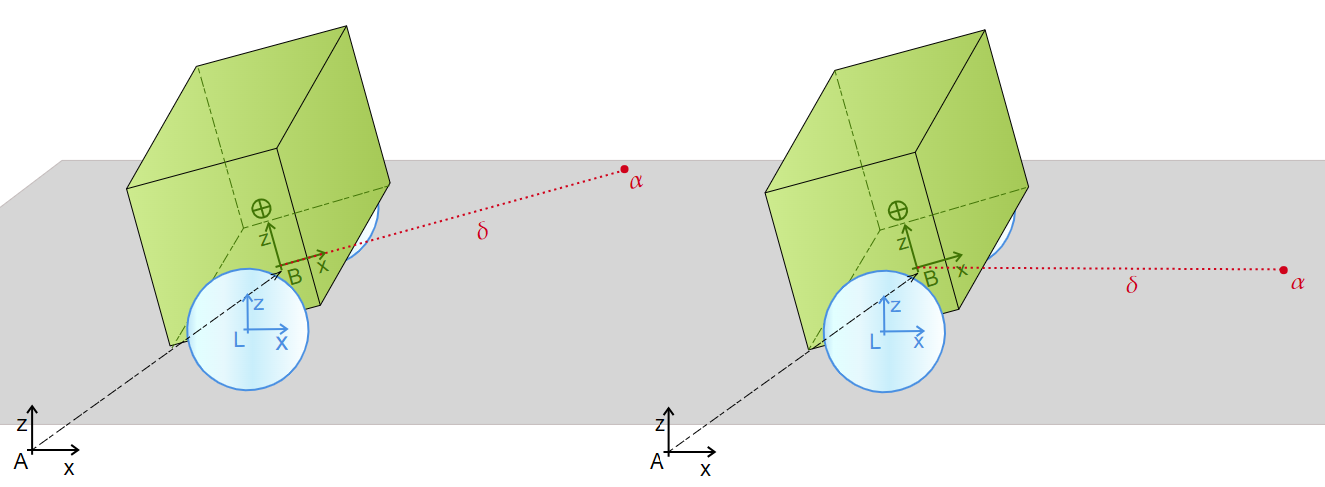
\includegraphics[width=0.85\linewidth]{accelerations decoupling.png}
    \caption{Accelerations decoupling.}
    \label{fig:accelerations decoupling}
\end{figure}

Also in this case we cannot directly impose a function of the robot configuration, but we have to derive twice the Equation \eqref{eq:control point generic} to end up in the control point acceleration.

The control point velocity is given by 

\begin{equation}
{}^{A} \dot{\bm{\alpha}} = \frac{d}{dt} ({}^{A} \bm{\alpha}) = {}^{A} \dot{\mathbf{P}} + {}^{A} \dot{R}_B^{xy} {}^{B} \bm{\delta}
\label{eq:control point velocity}
\end{equation}

and its acceleration is given by

\begin{equation}
{}^{A} \ddot{\bm{\alpha}} = \frac{d}{dt} ({}^{A} \bm{\dot{\alpha}}) = {}^{A} \ddot{\mathbf{P}} + {}^{A} \ddot{R}^{xy}_{B} {}^{B} \bm{\delta}
\label{eq:control point acceleration} 
\end{equation}

The complete derivation of the equation can be found in \cref{ch:Appendix}, here the final formulation of the control point acceleration is reported as affine function of the robot's generalized acceleration

\begin{equation}
\begin{aligned}
{}^{A} \ddot{\bm{\alpha}}_{xy} = & \; S_{v}J_{B}\dot{\bm{\nu}} - {}^{A} \dot{R}^{xy}_{B} ({}^{B}\bm{\delta}) ^\wedge S_{\omega}{}^{B}X_{B[A]}J_{B} \bm{\nu} \\
& - {}^{A} R^{xy}_{B}({}^{B}\bm{\delta})^\wedge S_{\omega}{}^{B} \dot{X}_{B[A]}J_{B} \bm{\nu} - {}^{A} R^{xy}_{B}({}^{B}\bm{\delta})^\wedge S_{\omega}{}^{B}X_{B[A]}J_{B} \dot{\bm{\nu}}.
\end{aligned}
\label{eq:control point acceleration affine}
\end{equation}

Also for this task, similarly to what has already been done in \cref{subsec:Self-Balancing Task} we have to define the error function to be minimized by the controller as stated in Equation \eqref{eq: Task equation with Jacobians}.

A simple manipulation of Equation \eqref{eq:control point acceleration affine}, defining the task Jacobian as

\begin{equation}
    J_{T_{\alpha}} = S_{v}J_{B} - {}^{A} R^{xy}_{B}({}^{B}\bm{\delta})^\wedge S_{\omega}{}^{B}X_{B[A]}J_{B}
    \label{eq: Tracking Task Jacobian}
\end{equation}

leads to 

\begin{equation*}
     \ddot{\bm{\alpha}}_{xy} = J_{T_{\alpha}}{\bm{\nu}} - J_{T_{\alpha}}\bm{\nu}.
\end{equation*}

Adopting the definition of desired acceleration provided in Equation \eqref{eq: Desired Acceleration}

\begin{equation}
    \ddot{\bm{\alpha}}_{xy}^{*} = \ddot{\bm{\alpha}}_{xy}^{n} -K_{d\alpha}(\dot{\bm{\alpha}}_{xy}-\dot{\bm{\alpha}}_{xy}^{n}) -K_{p\alpha}(\bm{\alpha}_{xy} - \bm{\alpha}_{xy}^{n})
    \label{eq: Alpha Desired Acceleration}
\end{equation}

where $K_{p\alpha}$ and $K_{d\alpha}$ are $2 \times 2$ diagonal matrices such as

\begin{equation}
    K_{p\alpha} = \begin{bmatrix}
        k_{p\alpha_x} & 0 \\
        0 & k_{p\alpha_y}
    \end{bmatrix}; K_{d\alpha} = \begin{bmatrix}
        k_{d\alpha_x} & 0 \\
        0 & k_{d\alpha_y}
    \end{bmatrix}.
\end{equation}

The final error function used for trajectory tracking control inside the TSID is 

\begin{equation}
   \mathbf{e(\bm{\alpha}_{xy},t)} =J_{T_{\alpha}}{\dot{\bm{\nu}}} - \dot{J}_{T_{\alpha}}\bm{\nu} - \ddot{\bm{\alpha}}_{xy}^{*} 
    \label{eq: Tracking error task}.
\end{equation}

\section{Constraints definition}
\label{sec:Constraints definition}

Once the tasks are defined, what is still missing is the formulation of the constraints. 
Our control problem requires three main constraints that are as follows:

\begin{itemize}
    \item Robot's dynamic equation
    \item Pure rolling contact constraint
    \item Forces friction cone constraint
\end{itemize}

The first has already been discussed in \cref{sec:E-Cargo Dynamical model}, while the others will be addressed in this section. 

\subsection{Pure Rolling Constraint}
\label{subsec:Pure Rolling Constraint}

We have seen in \cref{subsec:Constraints model} how a general rigid contact constraint is modeled.
Here the difference is that we cannot constrain the contact point to remain fixed for the whole contact duration, but we have to constrain its acceleration to be the desired one that guarantees rolling without slipping.

\begin{figure}
    \centering
    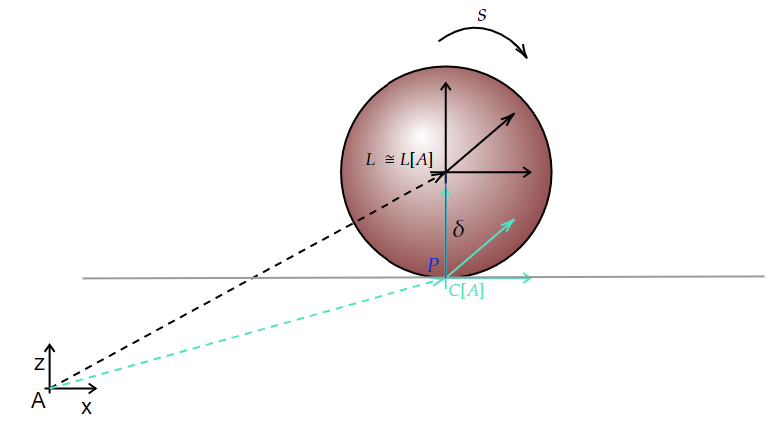
\includegraphics[width=0.65\linewidth]{Pure Rolling.png}
    \caption{Rolling kinematics.}
    \label{fig:Rolling kinematics}
\end{figure}

According to Figure \ref{fig:Rolling kinematics}, we define a generic point ${}^{A}\mathbf{P}_C$ that belongs to the circumference of the wheel and rotates together with the wheel's reference frame $L$

The point is kinematically defined as:

\begin{equation}
   {}^{A}\mathbf{P}_C = {}^{A} \mathbf{P}_{L} + {}^{A}R_{L} {}^{L}\bm{\delta} 
    \label{eq:Contact Point Position}
\end{equation}

and so its velocity is:

\begin{equation}
    {}^{A}\dot{\mathbf{P}}_{C} = {}^{A} \dot{\mathbf{P}}_{L} + {}^{A} \bm{\omega}^{\wedge{}}_{A,L} {}^{A}R_{L} {}^{L}\bm{\delta}. 
    \label{eq:Contact Point Velocity}
\end{equation}

Now, if we assume that at the instant considered, this point finds itself in the contact point between the wheel and the terrain, we can state that:

\begin{equation*}
    {}^{A}R_{L} {}^{L}\bm{\delta} = -r \mathbf{e_{3}}
\end{equation*}

where $r$ is the radius of the wheel.

If we substitute this equality inside the Equation \eqref{eq:Contact Point Velocity}, we can then impose the instantaneous velocity of a such defined point equal to zero to guarantee no slipping.

\begin{equation}
{}^{A}\dot{\mathbf{P}}_{C} = {}^{A} \dot{\mathbf{P}}_{L} - r {}^{A} \bm{\omega}^{\wedge{}}_{A,L} \mathbf{e_{3}} = 0.
\label{eq:Rolling velocity constraint}
\end{equation}

From this equation, we can obtain the expression for ${}^{A} \dot{\mathbf{P}}_{L}$, which is: 

\begin{equation}
{}^{A} \dot{\mathbf{P}}_{L} = r {}^{A} \bm{\omega}^{\wedge{}}_{A,L} \mathbf{e_{3}}.
\end{equation}

Deriving this expression, we end up in the constrain that we want to impose on the accelerations:

\begin{equation}
{}^{A} \ddot{\mathbf{P}}_{L} = r {}^{A} \dot{\bm{\omega}}^{\wedge{}}_{A,L} \mathbf{e_{3}}.
\end{equation}

And this relation is valid in mixed representation.

Also in this case the complete derivation of the equation can be found in \cref{ch:Appendix}, here just the final formulation of the contact point acceleration is reported as a function of the robot's generalized acceleration.

\begin{equation}
 (S_{v} J_{L} + r\mathbf{e_{3}}^{\wedge{}} S_{\omega} J_{L}) \dot{\bm{\nu}} + (r\mathbf{e_{3}}^{\wedge{}} S_{\omega} + S_{v}) \dot{J}_{L} \bm{\nu} = 0.
\label{eq: Pure Rolling Acceleration Constraint}
\end{equation}

At this point we group together some terms of Equation \eqref{eq: Pure Rolling Acceleration Constraint}, defining the constraint Jacobian as

\begin{equation}
    J_{R} = S_{v} J_{L} + r\mathbf{e_{3}}^{\wedge{}} S_{\omega} J_{L}.
    \label{eq: Rolling Jacobian}
\end{equation}

The final constraint formulation used inside the TSID is 

\begin{equation}
   \mathbf{c(\bm{q},t)} = J_{R}\bm{\dot{\nu}} + \dot{J}_R\bm{\nu} = 0.
    \label{eq: Rolling TSID contraint}
\end{equation}

\subsection{Forces Friction Cone}
\label{subsec:Forces Friction Cone}

We can sketch at this point a first version of the control problem, given the preliminary structure obtained by combining Equations \eqref{eq:e-Cargo dynamic equation} \eqref{eq: Pitch error task} \eqref{eq: Tracking error task} \eqref{eq: Rolling TSID contraint}.

\begin{center}
$\underset{\bm{\dot{\nu},{}_{B}\mathbf{f},\bm{\tau}}}{\text{argmin}} (W_{\alpha}\|J_{T_{\alpha}}{\dot{\bm{\nu}}} - \dot{J}_{T_{\alpha}}\bm{\nu} - \ddot{\bm{\alpha}}_{xy}^{*}\|^{2} + w_{\theta}\| J_{T_P}{\dot{\bm{\nu}}} - \dot{J}_{T_P}\bm{\nu} - \ddot{\theta}^{*} \|^{2})$

\text{subject to}

\end{center}

\begin{equation}
\begin{cases}
        M(\mathbf{q})\dot{\bm{\nu}} + C(\mathbf{q},\bm{\nu})\bm{\nu} + \mathbf{g}(\mathbf{q}) = S\bm{\tau} + J^{T}_{C} {}_{B}\mathbf{f} \\
        J_{R}\bm{\dot{\nu}} + \dot{J}_R\bm{\nu} = 0
\end{cases}
\label{eq: First TSID Structure}
\end{equation}

Notice that $W_{\alpha}$ is a diagonal matrix with task weights 

\begin{equation*}
    W_{\alpha} = \begin{bmatrix}
        w_{\alpha_x} & 0 \\
        0 & w_{\alpha_y}
    \end{bmatrix}.
\end{equation*}

There is still something missing:
In our control framework the contact forces are also optimization variables, but looking at Equations \eqref{eq: First TSID Structure}, at this level the controller is free to choose whatever values for the contact wrench ${}_{B}\mathbf{f}$ which respect the robot dynamic.
In real applications, we know that to ensure rolling without slipping, the forces have to lie inside the friction cone, which is generally defined as \cite{Pretorius-et-al}:

\begin{equation}
\begin{cases}
  f_z > f_z^{min} \geq 0\\
\\
 \sqrt{f_x ^{2} + f_y ^{2}} < \mu_c f_z \\
\end{cases}
\label{eq:nonlinear friction cone}
\end{equation}

where $\mu_c$ is the static friction coefficient and $f_x, f_y, f_z$ are respectively the $1^{st}, 2^{nd}, 3^{rd}$ components of a single 3D contact wrench.

The control problem we aim to set up is a Quadratic Program (QP), which can only accept affine constraints. Therefore, the friction cone is typically approximated by a generic polyhedron with an arbitrary number of sides ass shown in Figure (\ref{fig:Friction Cone Approximation}).

\begin{figure}
    \centering
    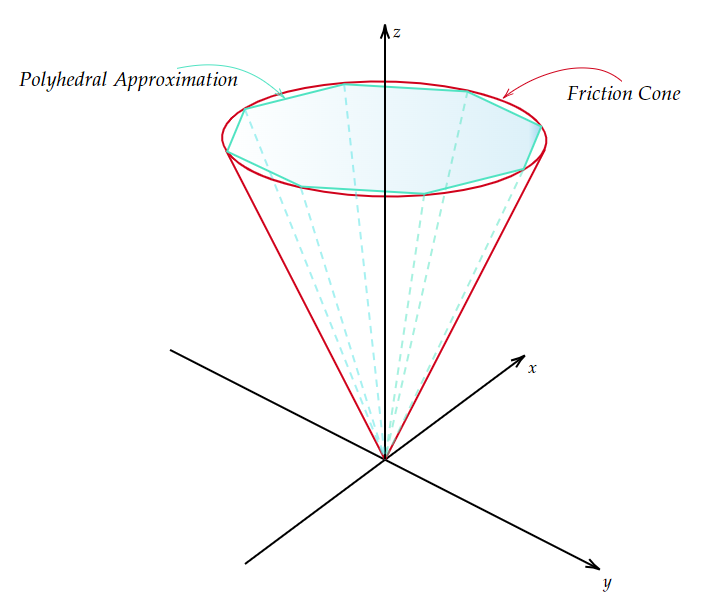
\includegraphics[width=0.5\linewidth]{Friction cone.png}
    \caption{Friction Cone Approximation.}
    \label{fig:Friction Cone Approximation}
\end{figure}

This approximation allows us to pass from the system of equations \eqref{eq:nonlinear friction cone}
to a matrix inequality like

\begin{equation}
    A_{f}{}_{B}\mathbf{f} < \mathbf{b}_{f}
\label{eq:Linear friction cone}
\end{equation}

where the size of the matrix $A_{f}$, and so the number of inequalities, depends on the number of the sides of the polyhedron; for our application in particular, we choose a polyhedron with eight sides.
Equation \eqref{eq:Linear friction cone} is then incorporated into the system in Equation \eqref{eq: First TSID Structure}.

\section{Nominal Trajectory Planner}
\label{sec:Nominal Trajectory Planner}

The version of the control problem in Equation \eqref{eq: First TSID Structure} with the addition of the inequality constraints in Equation \eqref{eq:Linear friction cone}, if properly tuned, could give some good results only if the performance requirements are low. 
This can be easily understood by examining the formulations of the desired accelerations in Equations \eqref{eq: Alpha Desired Acceleration} and \eqref{eq: Pitch Desired Acceleration}, which are written again here for clarity

\begin{equation*}
    \ddot{\bm{\alpha}}_{xy}^{*} = \ddot{\bm{\alpha}}_{xy}^{n} -K_d(\dot{\bm{\alpha}}_{xy}-\dot{\bm{\alpha}}_{xy}^{n}) -K_p(\bm{\alpha}_{xy} - \bm{\alpha}_{xy}^{n})
\end{equation*}

\begin{equation*}
    \ddot{\theta}^{*} = \ddot{\theta}^{n} -K_d(\dot{\theta}-\dot{\theta}^{n}) -K_p(\theta - \theta^{n})
\end{equation*}

The \textit{nominal trajectories} denoted with the apex $'n'$, are by definition feasible user defined trajectories that we want our robot to follow; this problem is dynamically coupled in the sense that the nominal trajectories that we want to impose for the stabilization ($\theta^{n}, \dot{\theta}^{n}, \ddot{\theta}^{n}$) have to be a function of the ones imposed or the tracking ($\bm{\alpha}_{xy}^{n}, \dot{\bm{\alpha}}_{xy}^{n}, \ddot{\bm{\alpha}}_{xy}^{n}$).

\begin{figure}
    \centering
    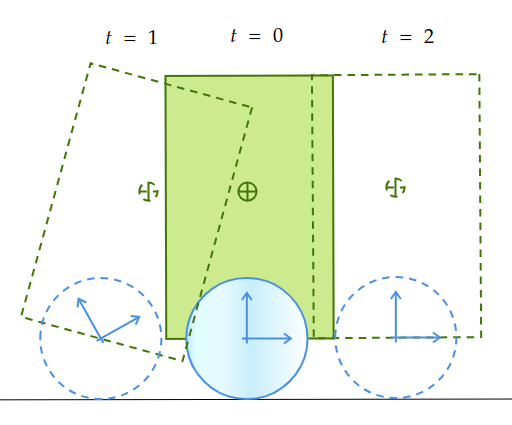
\includegraphics[width=0.6\linewidth]{nominal trajectory coupling.png}
    \caption{Nominal Trajectory Coupling.}
    \label{fig:Nominal Trajectory Coupling}
\end{figure}

With reference to Figure \ref{fig:Nominal Trajectory Coupling} we want to highlight that if the robot has to move on the right starting from an initial condition in which it is standstill with pitch angle $\theta =0$, it has to adjust the pitch angle according to the acceleration that we want on the rightward direction.
This means that if we do not define a proper relationship between the nominal trajectories, the controller will always attempt to minimize the largest error. However, every time the tracking error decreases, the stabilization error increases, and vice versa, leading to undesired oscillatory behavior that significantly reduces the achievable performances. 

This problem can be addressed in different ways that will be briefly discussed in \cref{ch:conclusions}, here we adopted a simple but effective solution: knowing that the goal is finding a relation of the type: $\theta^{n} = f (\ddot{\bm{\alpha}}_{xy}^{n}, t)$, we choose as $\theta^{n}$ the output of a PI controller on the in-plane velocity ($\dot{\alpha}_{x} + \dot{\alpha}_{y}$)

\begin{equation}
\theta^{n} =K_P((\dot{\alpha}_{x}^{n}+\dot{\alpha}_{y}^{n}) - (\dot{\alpha}_{x} + \dot{\alpha}_{y})) + K_I \int ((\dot{\alpha}_{x}^{n}+\dot{\alpha}_{y}^{n}) -(\dot{\alpha}_{x} + \dot{\alpha}_{y})) \  dt .
\label{eq:simple planner version}
\end{equation}

The PI controller in Equation \eqref{eq:simple planner version} acts as a linear nominal trajectory planner.
A simple block diagram of the entire control architecture is represented in Figure \ref{fig:TSID Control Block Diagram}

\begin{figure}
    \centering
    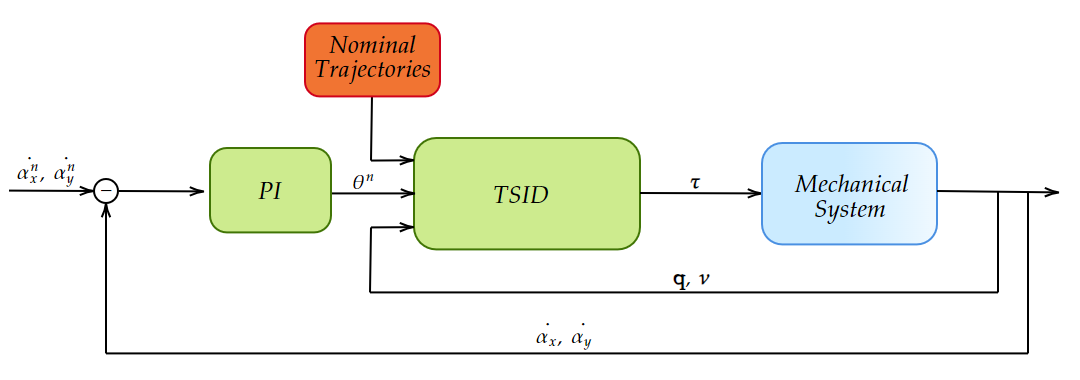
\includegraphics[width=1\linewidth]{Overall Scheme.png}
    \caption{TSID Control Block Diagram.}
    \label{fig:TSID Control Block Diagram}
\end{figure}


\section{Control Problem Formulation}
\label{sec:Control Problem Formulation}

The control problem now has all the elements and can be formulated in its complete version.

We first define the LSP formulation, and then pass to the more generic QP formulation.
\vspace{12pt}
\begin{center}
{\large \textbf{LSP Formulation}}
\end{center}

\begin{center}
$\underset{\bm{\dot{\nu},{}_{B}\mathbf{f},\bm{\tau}}, \bm{\xi}}{\text{argmin}} (W_{\alpha}\|J_{T_{\alpha}}{\dot{\bm{\nu}}} - \dot{J}_{T_{\alpha}}\bm{\nu} - \ddot{\bm{\alpha}}_{xy}^{*}\|^{2} + w_{\tau}\| \tau_L \|^{2} + w_{\tau}\| \tau_R \|^{2} + w_{\xi} \| \xi \|^{2} + {}_{B}\mathbf{f}^{T} \lambda I {}_{B}\mathbf{f})$

\text{subject to}

\end{center}

\begin{equation}
\begin{cases}
        M(\mathbf{q})\dot{\bm{\nu}} + h(\mathbf{q},\bm{\nu}) = S\bm{\tau} + J^{T}_{C} {}_{B}\mathbf{f} \\
        J_{R}\bm{\dot{\nu}} + \dot{J}_R\bm{\nu} = 0 \\
        J_{T_P}{\dot{\bm{\nu}}} - \dot{J}_{T_P}\bm{\nu} - \ddot{\theta}^{*} + \xi = 0 \\
        A_{f}{}_{B}\mathbf{f} < \mathbf{b}_{f} \\
        lb_{\xi} \leq \xi \leq ub_{\xi}
\end{cases}
\label{eq: LSP Formulation}
\end{equation}

With respect to the preliminary formulation given in Equation \eqref{eq: First TSID Structure}, some changes have been made

\begin{itemize}
    \item The stabilization problem involving the Equation \eqref{eq: Pitch error task} has been moved from the cost function to the constraints, with the addition of a slack variable $\xi$
    \item A double bounded inequality has been used to constrain the value of the slack variable $\xi$ which is then minimized inside the cost function as $w_{\xi} \| \xi \|^{2}$
    \item A \textit{regularization} term has been added on the contact forces with regularization coefficients $\lambda_{i}$ 
\end{itemize}

Since the Optimization-Based Control Problem is solved using a QP solver, the LS structure needs to be rearranged to conform to the conventional QP matrix formulation.
The complete derivation is performed in the \cref{ch:Appendix}, while here is reported just the final QP control structure


\vspace{12pt}
\begin{center}
{\large \textbf{QP Formulation}}
\end{center}

\begin{center}
$\underset{\bm{\dot{\nu},{}_{B}\mathbf{f},\bm{\tau}}, \bm{\xi}}{\text{argmin}} (\frac{1}{2} \mathbf{v}^{T} H \mathbf{v} + \mathbf{c}^{T} \mathbf{v})$
\text{subject to}
\end{center}

\begin{equation}
\begin{Bmatrix} 
-h(\mathbf{q},\bm{\nu})\\
-\dot{J_{R}}\bm{\nu} \\
\dot{J}_{T_P}\bm{\nu} + \ddot{\theta}^{*}\\
-\bm{\infty} \\
ub_{\xi} \\
\end{Bmatrix} \leq \begin{bmatrix} 
M(\mathbf{q}) & -J_c^{T} & -S & 0 \\
J_{R} & 0 & 0  & 0\\
J_{T_P} & 0 & 0  & 1\\
0 & A_{f} & 0 & 0\\
0 & 0 & 0 & 1 \\
\end{bmatrix} \begin{Bmatrix} 
\dot{\bm{\nu}} \\
{}_{B}\mathbf{f} \\
\bm{\tau}  \\
\xi \\
\end{Bmatrix} \leq \begin{Bmatrix} 
-h(\mathbf{q},\bm{\nu})\\\
-\dot{J_{R}}\bm{\nu}\\
\dot{J}_{T_P}\bm{\nu} + \ddot{\theta}^{*} \\
\mathbf{b}_{f} \\
ub_{\xi} \\
\end{Bmatrix}
\label{eq: QP Formulation}
\end{equation}

\chapter{Implementation and Results}
\label{ch:chapter_five}%
% The \label{...}% enables to remove the small indentation that is generated, always leave the % symbol.

The whole work has been done in Matlab and Simulink and the overall scheme is represented in Figure \ref{fig:SIMULINK complete Model}

\begin{figure}
    \centering
    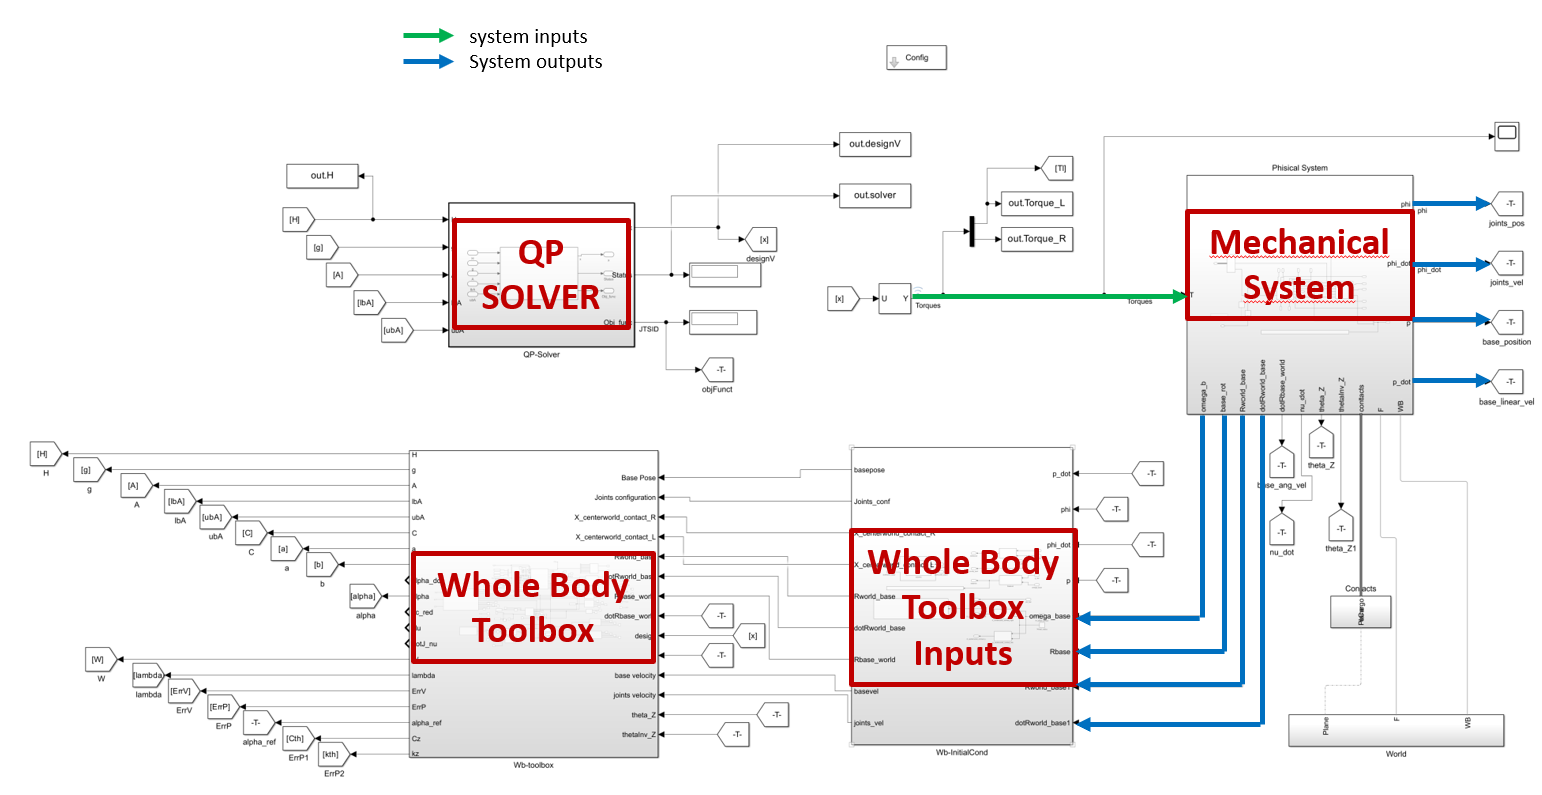
\includegraphics[width=1\linewidth]{Simulink overall model.png}
    \caption{Simulink complete Model.}
    \label{fig:SIMULINK complete Model}
\end{figure}

\section{Simulink modeling}
\label{sec:Simulink modeling}

Without going into the details of all the sub-systems involved, it can be useful to have a look to some specific blocks that have been used for modeling, sensing and control.
The simulation results reported in this chapter consider the E-Cargo loaded at its maximum capacity, with a total mass of 60 kg, and assuming a friction coefficient $\mu_c = 0.5$ between the wheels and the terrain.

\subsection{Robot URDF model}
\label{subsec:Robot URDF model}

\begin{figure}
  \centering
  \begin{minipage}{0.35\textwidth}
    \centering
    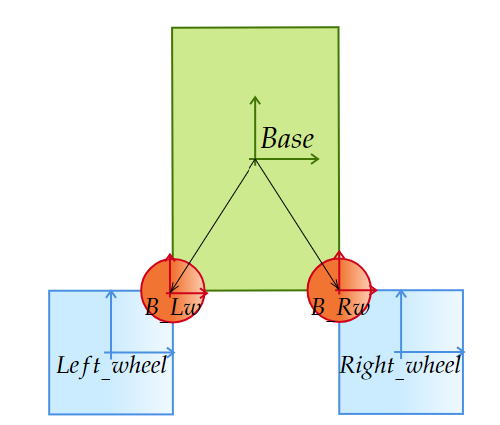
\includegraphics[width=1\linewidth]{Robot URDF model.png} % Adjust width as needed
  \end{minipage}%
  \begin{minipage}{0.55\textwidth}
    \small % Reduce font size for URDF code
    \begin{verbatim}
    <?xml version="1.0"?>
    <robot name="E-Cargo">
    
      <link name="base"> ... </link>
      <link name="left_wheel"> ... </link>
      <link name="right_wheel"> ... </link>
    
      <joint name="base_left" type="revolute"> ... </joint>
      <joint name="base_right" type="revolute"> ... </joint>
    
    </robot>
    \end{verbatim}
  \end{minipage}
  \caption{Robot URDF model.}
  \label{fig:Robot URDF model}
\end{figure}

The most important input of the simulation is the robot URDF file: an XML-based file format used to describe robots, humanoids in particular. It defines the structure, visual appearance, and physical properties of a robot's components such as links and joints with the assumption of rigid links and ideal joints already discussed in \cref{subsec: Links and Joints}.
Figure \ref{fig:Robot URDF model} provides a simplified sketch illustrating our URDF model, depicting a body with two wheels connected via two revolute joints. 
This input file is used both to create the robot block diagram in Simulink (as shown in Figure \ref{fig:Robot block diagram}), and to compute in real time all the matrices describing its dynamic through a Simulink toolbox named \textbf{Whole-Body Toolbox (Wb-Toolbox)}.

\begin{figure}
    \centering
    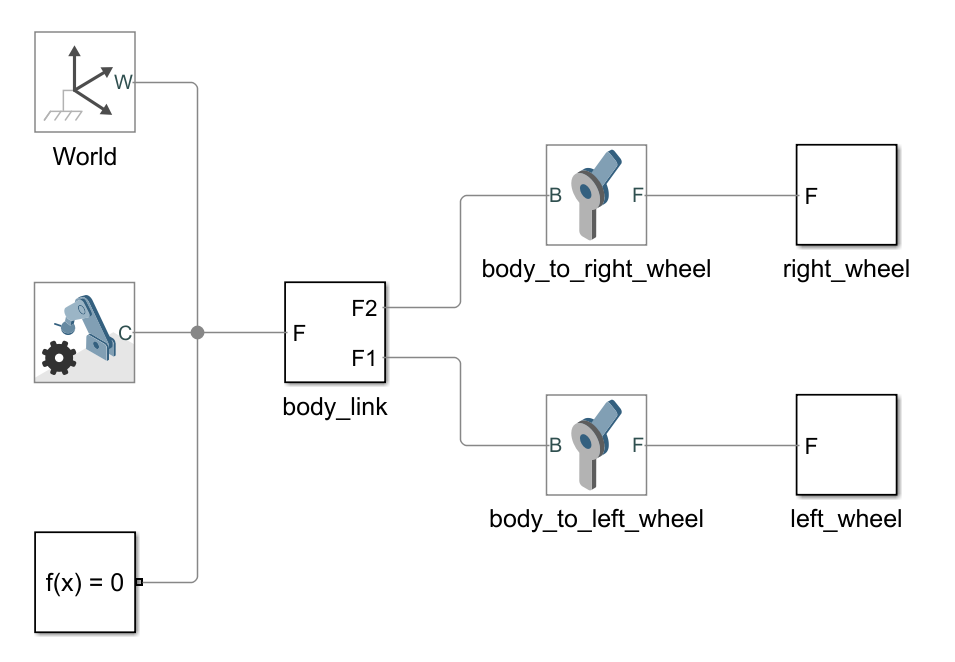
\includegraphics[width=0.5\linewidth]{Robot Block Diagram.png}
    \caption{Robot block diagram.}
    \label{fig:Robot block diagram}
\end{figure}

\subsection{Simulink blocks overview}
\label{subsec:Simulink blocks overview}

Once the robot has been created in the simulation environment, its contacts with the external world have been defined through the Simscape block \textit{Spatial Contact Force} (Figure \ref{fig:Spatial Contact Force block}).

\begin{figure}
    \centering
    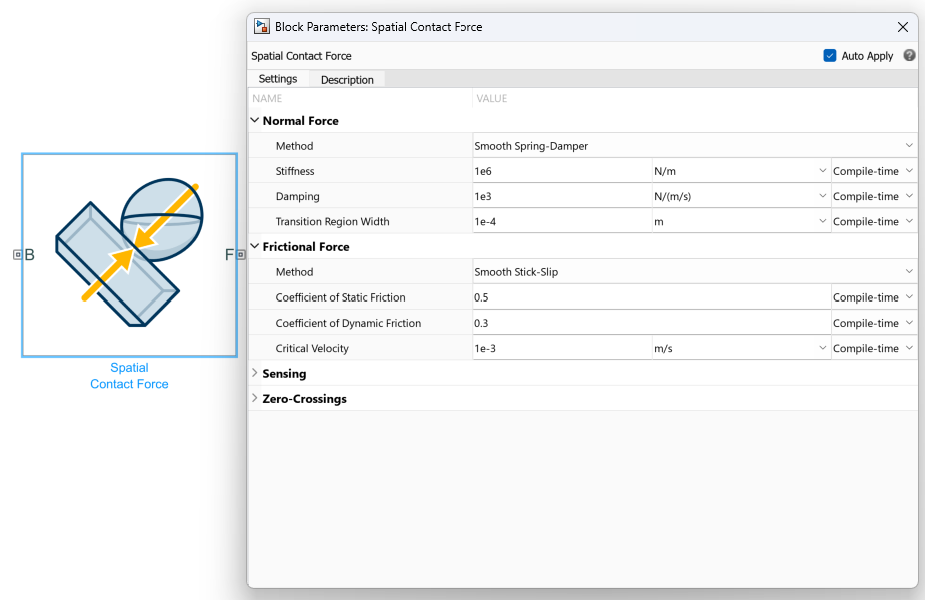
\includegraphics[width=0.7\linewidth]{Spatial Contact Force.png}
    \caption{Spatial Contact Force block.}
    \label{fig:Spatial Contact Force block}
\end{figure}

This block model the contact as rigids (spring-damper) coherently with our model assumption; in our simulation we assume just static friction between the wheels and the terrain for this moment, and the friction coefficient used as input for this block, is the same used for the friction cone constraint. 

The sensing of the all the needed reasonable feedbacks have been made through the block \textit{Transform Sensor}, (Figure \ref{fig:Transform Sensor Block}) which allows us to compute important time-dependent transformations between two frames named \textit{base} and \textit{follower}, and to project them in a third user-specified frame.
This last feature is very useful to change the representation switching from \textit{left trivialized}, \textit{right trivialized} and \textit{mixed}.

\begin{figure}
    \centering
    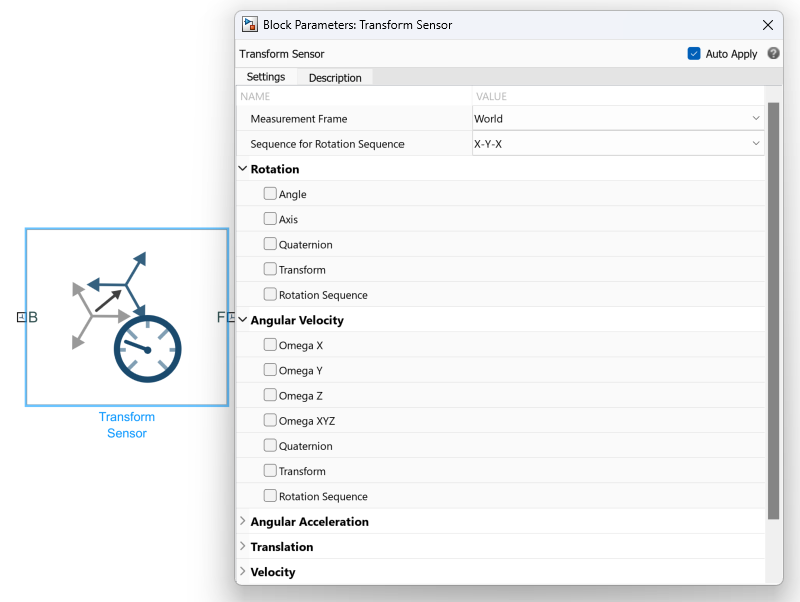
\includegraphics[width=0.7\linewidth]{Transform Sensor Block.png}
    \caption{Transform Sensor Block.}
    \label{fig:Transform Sensor Block}
\end{figure}

The last remark regards the block \textit{OSQP}: it uses the OSQP libraries to solve the optimization-based control problem given the inputs defined in \cref{sec:Converting Least-Squares to Quadratic Programming} and a maximum number of possible iterations.

\begin{figure}
    \centering
    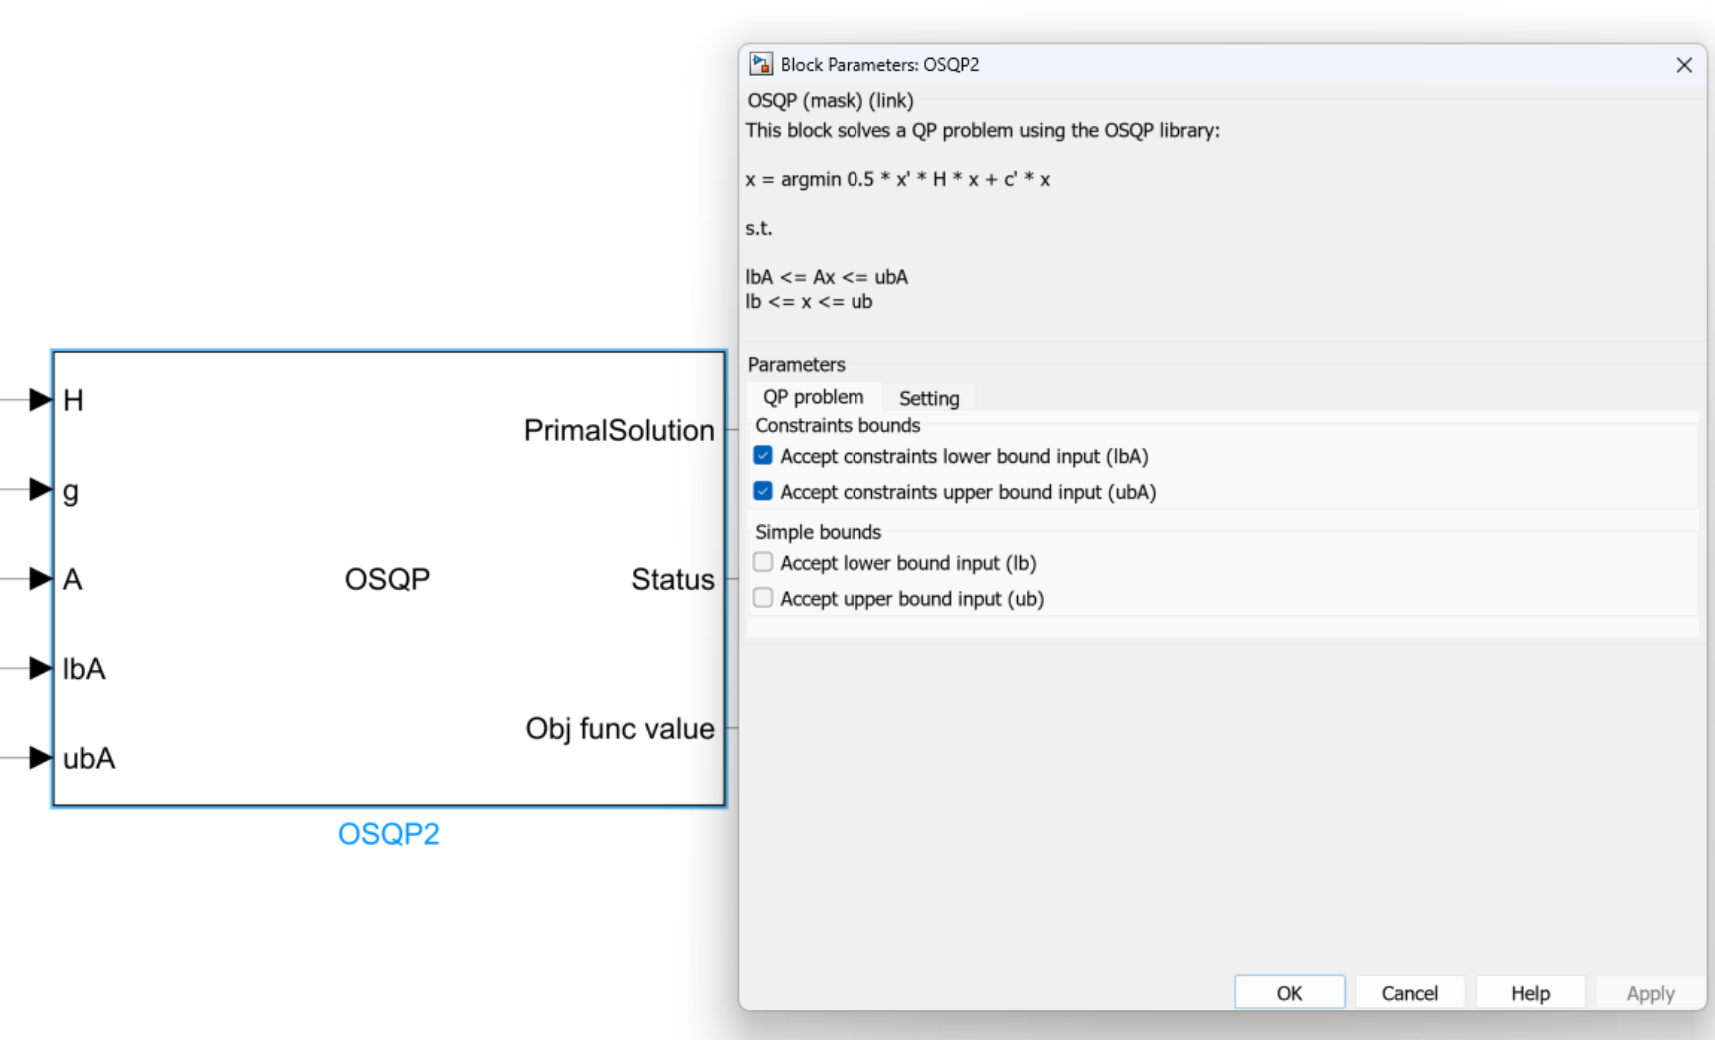
\includegraphics[width=0.8\linewidth]{OSQP.png}
    \caption{OSQP solver block.}
    \label{fig:OSQP solver block}
\end{figure}


\section{Simulation results}
\label{sec:Simulation results}

To validate our mathematical derivation of the controller we conducted some simulations involving different features that we want our E-Cargo to posses.
Simulating a real scenario, we found a set of parameters that, given the system model, does not change with respect to the different nominal trajectories and different requirements.

\subsection{Gain tuning}
\label{subsec:Gain tuning}

This type of controller requires proper tuning of certain user-defined parameters. In our case, we did not adopt a specific criterion for this; instead, we used a trial-and-error approach to find the best compromise between the initial swing-up performance of the E-Cargo and effective trajectory tracking.

\begin{table}[h!]
\centering
\setlength{\tabcolsep}{30pt} % Adjust the value to increase the distance
\large
\begin{tabular}{>{\bfseries}l l}
\textbf{Parameter} & \textbf{Value} \\
\hline
\multicolumn{2}{l}{\textit{TSID Controller Parameters}} \\
\hline
$K_{P\alpha_x}$ & 80 \\
$K_{P\alpha_x}$ & 80 \\
$K_{P\theta}$ & 100 \\
$K_{D\alpha_x}$ & 113.14 \\
$K_{D\alpha_x}$ & 113.14 \\
$K_{D\theta}$ & 70.7 \\
\hline
\multicolumn{2}{l}{\textit{QP Weights}} \\
\hline
$w_{\alpha_x}$ & 100 \\
$w_{\alpha_y}$ & 100 \\
$w_{\tau}$ & 1 \\
$w_{\xi}$ & 1 \\
$w_{\delta}$ & 1 \\
$\lambda$ & $1^{-3}$ \\
\hline
\multicolumn{2}{l}{\textit{PI Trajectory Planner}} \\
\hline
$K_{Pp}$ & 0.5 \\
$K_{Ip}$ & 0.1 \\
\end{tabular}
\caption{Set of Gains and Weights.}
\label{tab:Set of Gains and Weights}
\end{table}

\newpage
Given the set of parameters in Table \ref{tab:Set of Gains and Weights}, three different cases have been simulated:

\begin{enumerate}
    \item initial swing-up starting from $\theta = 25^{\circ}$

    With the same nominal trajectories in the $x$ direction, (Figure \ref{fig:Nominal trajectories x-direction}) two different nominal trajectories in the $y$ direction:
    \item nominal $y$ trajectory $=0$
    \item nominal $y$ trajectory $= A \sin{t}$
\end{enumerate}

\begin{figure}
    \centering
    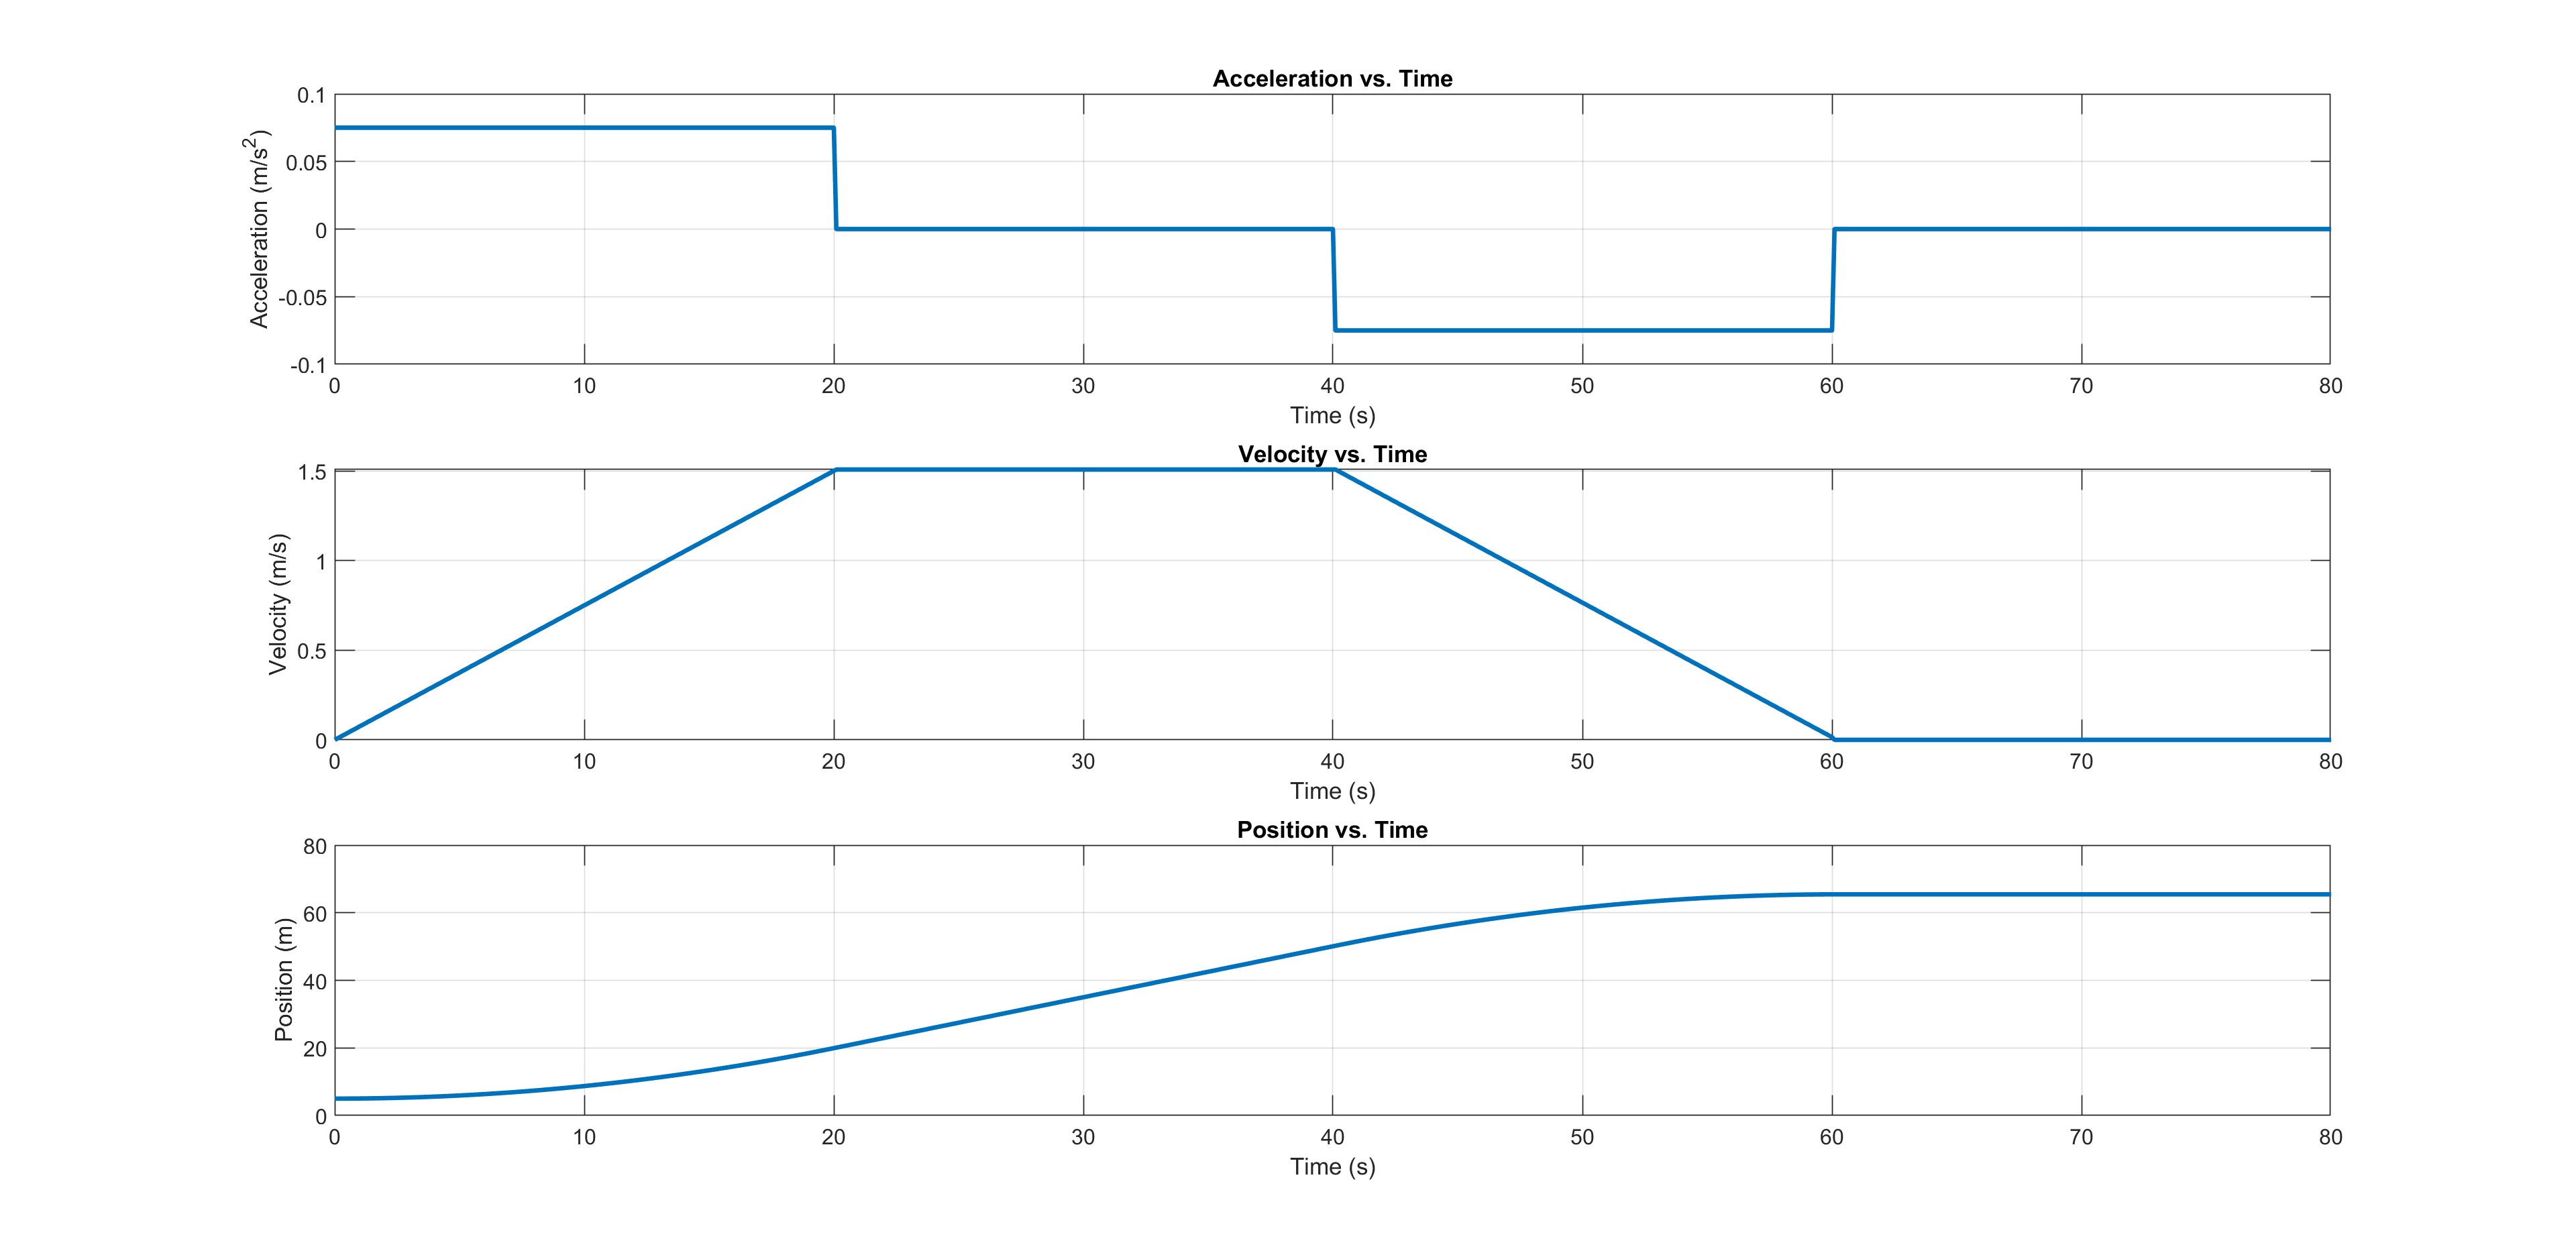
\includegraphics[width=1\linewidth]{Images/x-trajectory/Reference_trajectories.jpg}
    \caption{Nominal trajectories x-direction.}
    \label{fig:Nominal trajectories x-direction}
\end{figure}

The trajectory shown in Figure \ref{fig:Nominal trajectories x-direction} has been used to evaluate the controller's performance in the key phases: start, acceleration, deceleration, and stop; considering a cruise velocity of 1.5 $m/s$ which is close to the maximum allowed one.

\subsection{Swing-up}
\label{subsec:Swing-up}

The swing-up has been tested using nominal trajectories where the initial position of the control point is set with zero velocity and acceleration. Additionally, the nominal pitch angle velocity and acceleration are also set to zero.

In Figure \ref{fig:Swing-Up Position error} are shown in red the actual trajectories in position, while in blue are shown the nominal ones:
After a transient of $\approx$ 4 sec, the red curves follow the blue ones.

Figure \ref{fig:Swing-Up Velocity error} shows the velocity trajectories, using the same color criteria. It can be observed how the error between the actual and nominal velocities regulates the nominal pitch angle trajectory shown in Figure \ref{fig:Swing-Up Position error}.

\begin{figure}
    \centering
    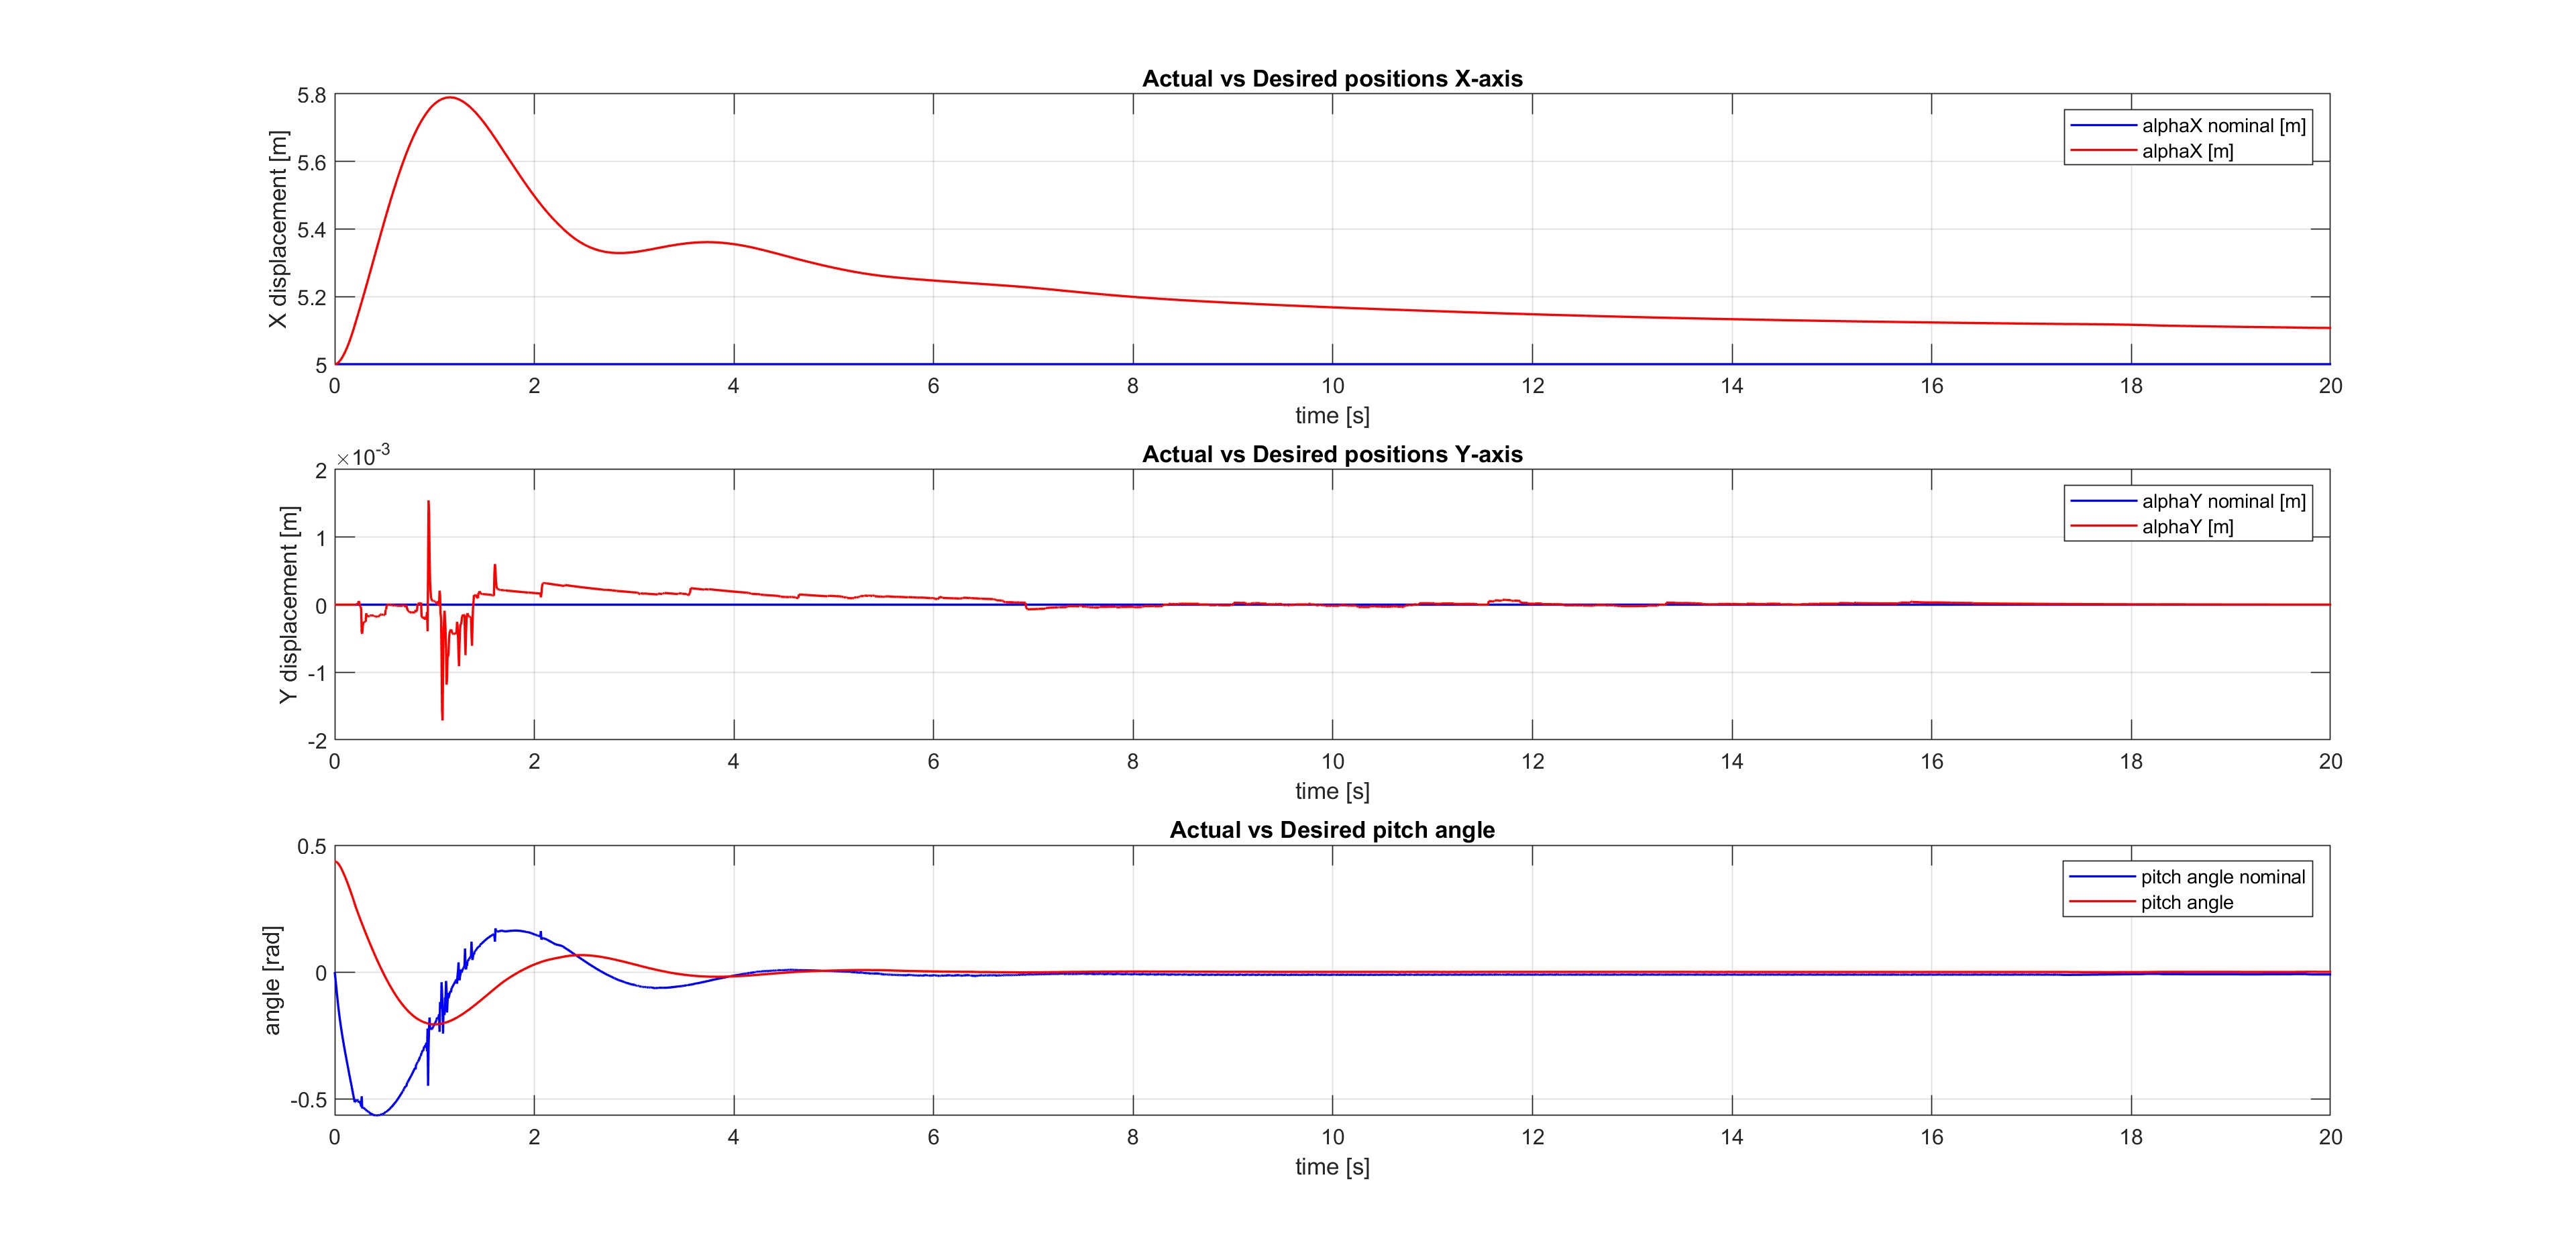
\includegraphics[width=1\linewidth]{Images/Swing-Up/Position_error.jpg}
    \caption{Swing-Up Position error.}
    \label{fig:Swing-Up Position error}
\end{figure}

\begin{figure}
    \centering
    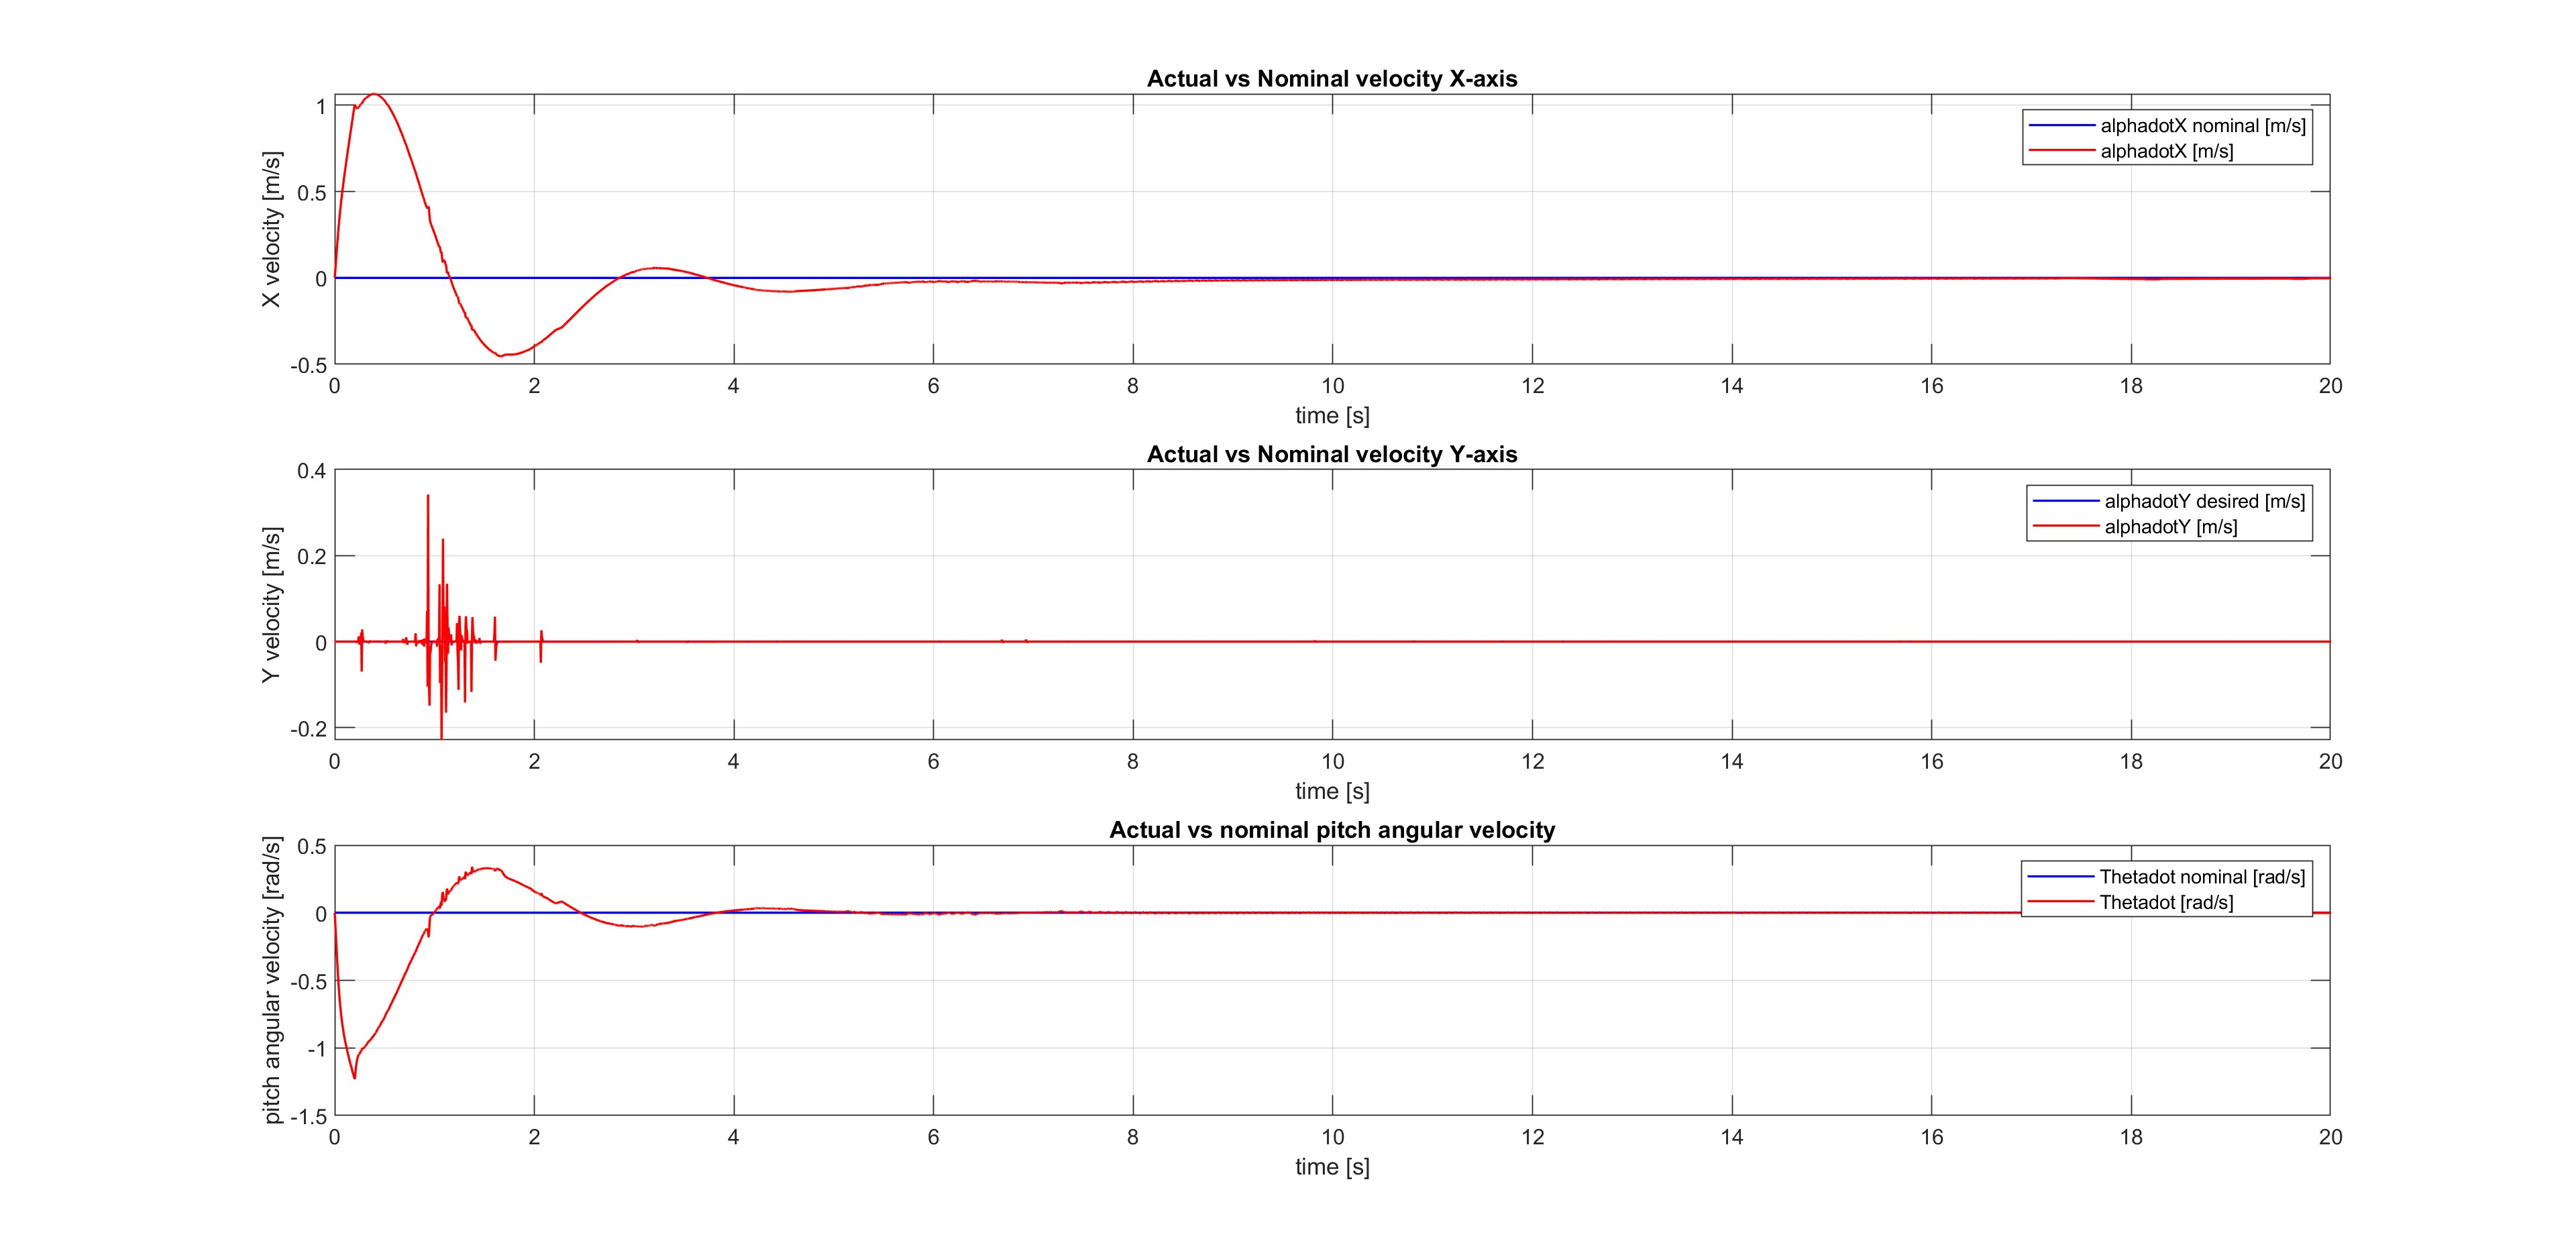
\includegraphics[width=1\linewidth]{Images/Swing-Up/Velocity_error.jpg}
    \caption{Swing-Up Velocity error.}
    \label{fig:Swing-Up Velocity error}
\end{figure}

\subsection{Straight Trajectory}
\label{subsec:Straight Trajectory}

The tracking has been tested by starting with the base in its upright position $\theta^{n} = 0$, considering that this is more difficult with respect to start with a pitch angle >0.

Apart for some mismatches corresponding to the points in which the acceleration profile is discontinuous, the red actual trajectories follows the nominal blue ones both in position (Figure\ref{fig:Straight trajectory Position error}) and in velocity (Figure\ref{fig:Straight trajectory Velocity error}).

\begin{figure}
    \centering
    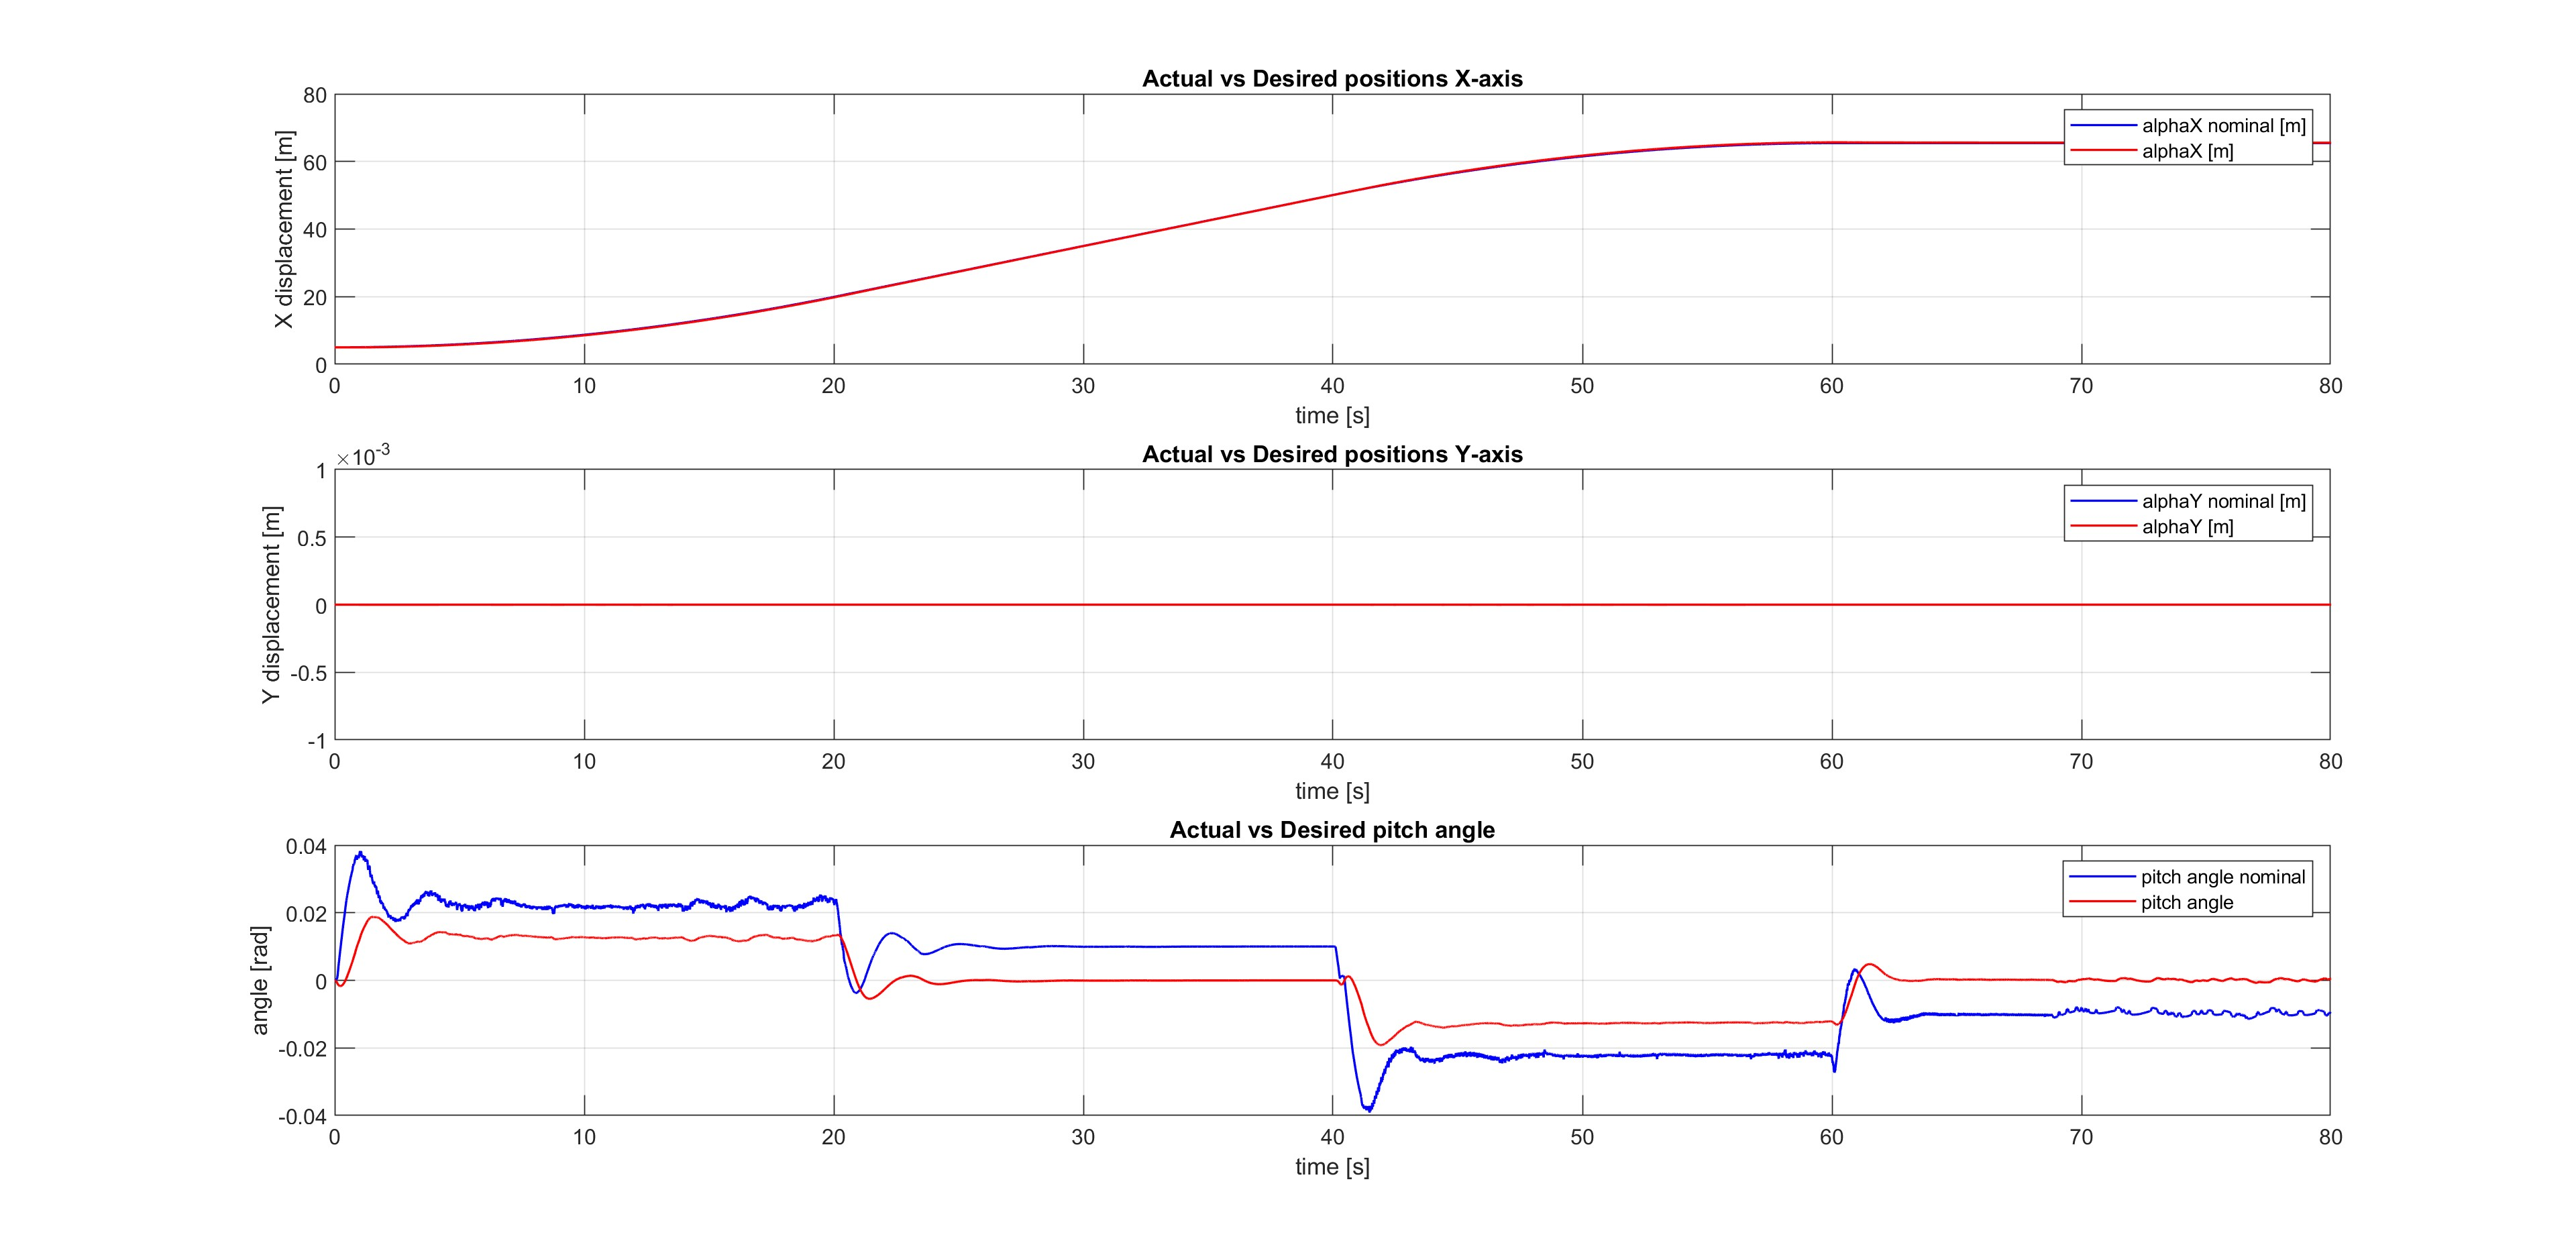
\includegraphics[width=1\linewidth]{Images/x-trajectory/Position_error.jpg}
    \caption{Straight trajectory Position error.}
    \label{fig:Straight trajectory Position error}
\end{figure}

\begin{figure}
    \centering
    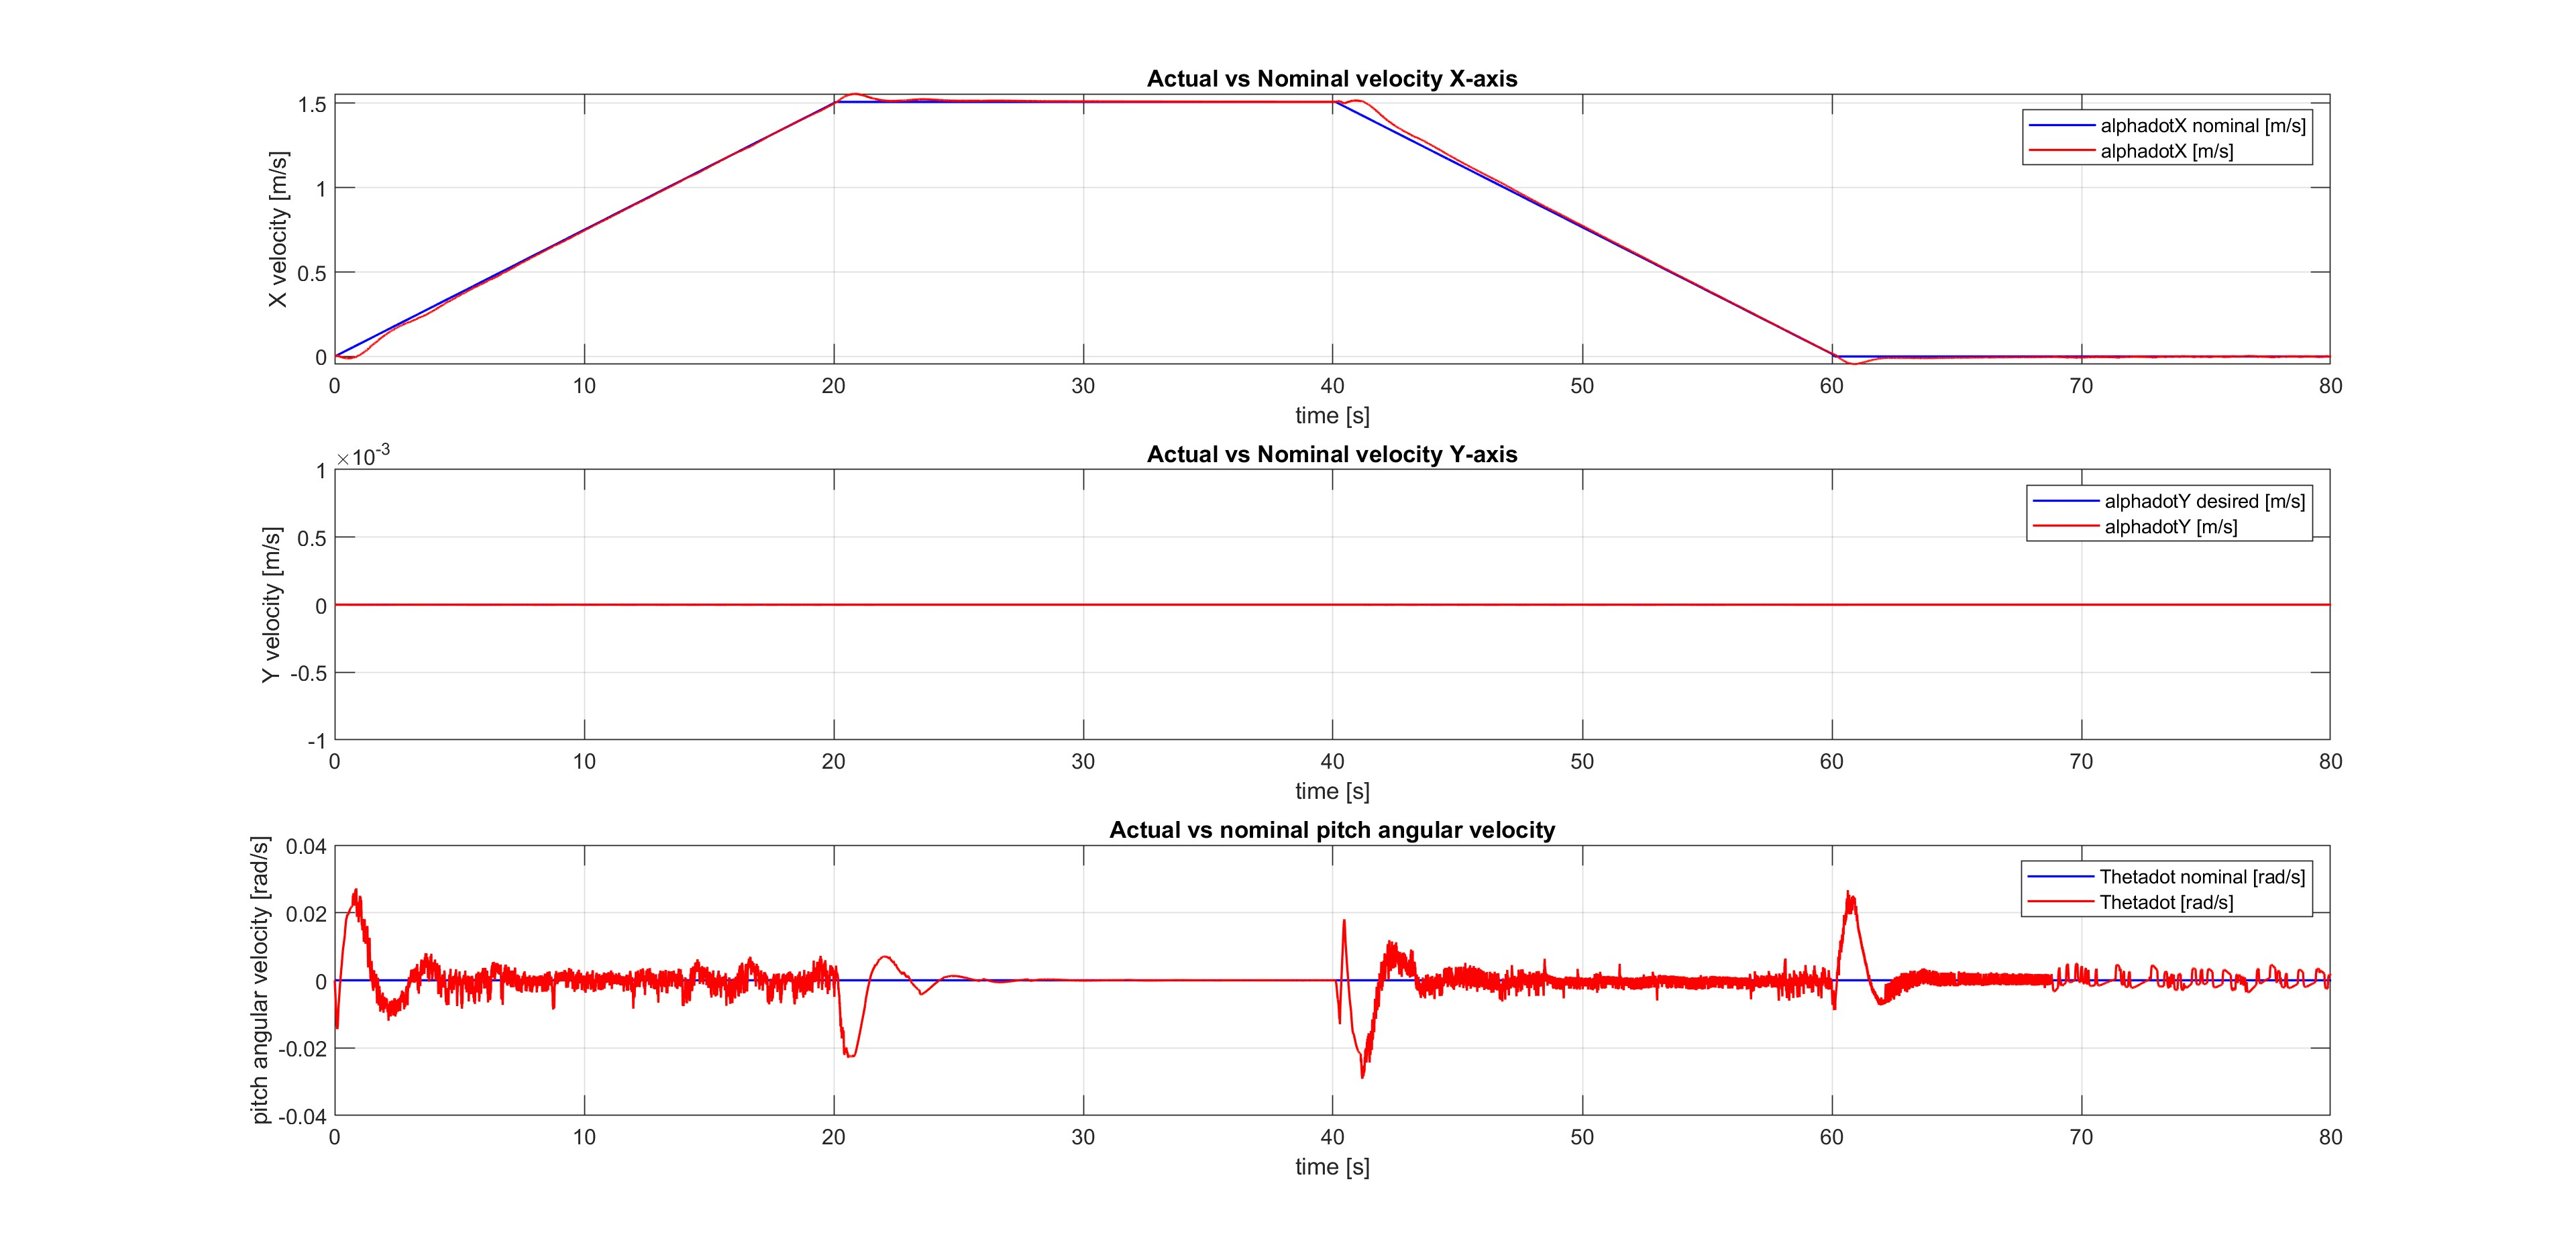
\includegraphics[width=1\linewidth]{Images/x-trajectory/Velocity_error.jpg}
    \caption{Straight trajectory Velocity error.}
    \label{fig:Straight trajectory Velocity error}
\end{figure}

\subsection{Sinusoidal Trajectory}
\label{subsec:Sinusoidal Trajectory}

To validate the decision regarding the choice of controlling a point different from the base, allowing for instantaneous velocity components along the y-axis, we tested a final trajectory involving a general sinusoidal nominal trajectory in the y direction.

\begin{figure}
    \centering
    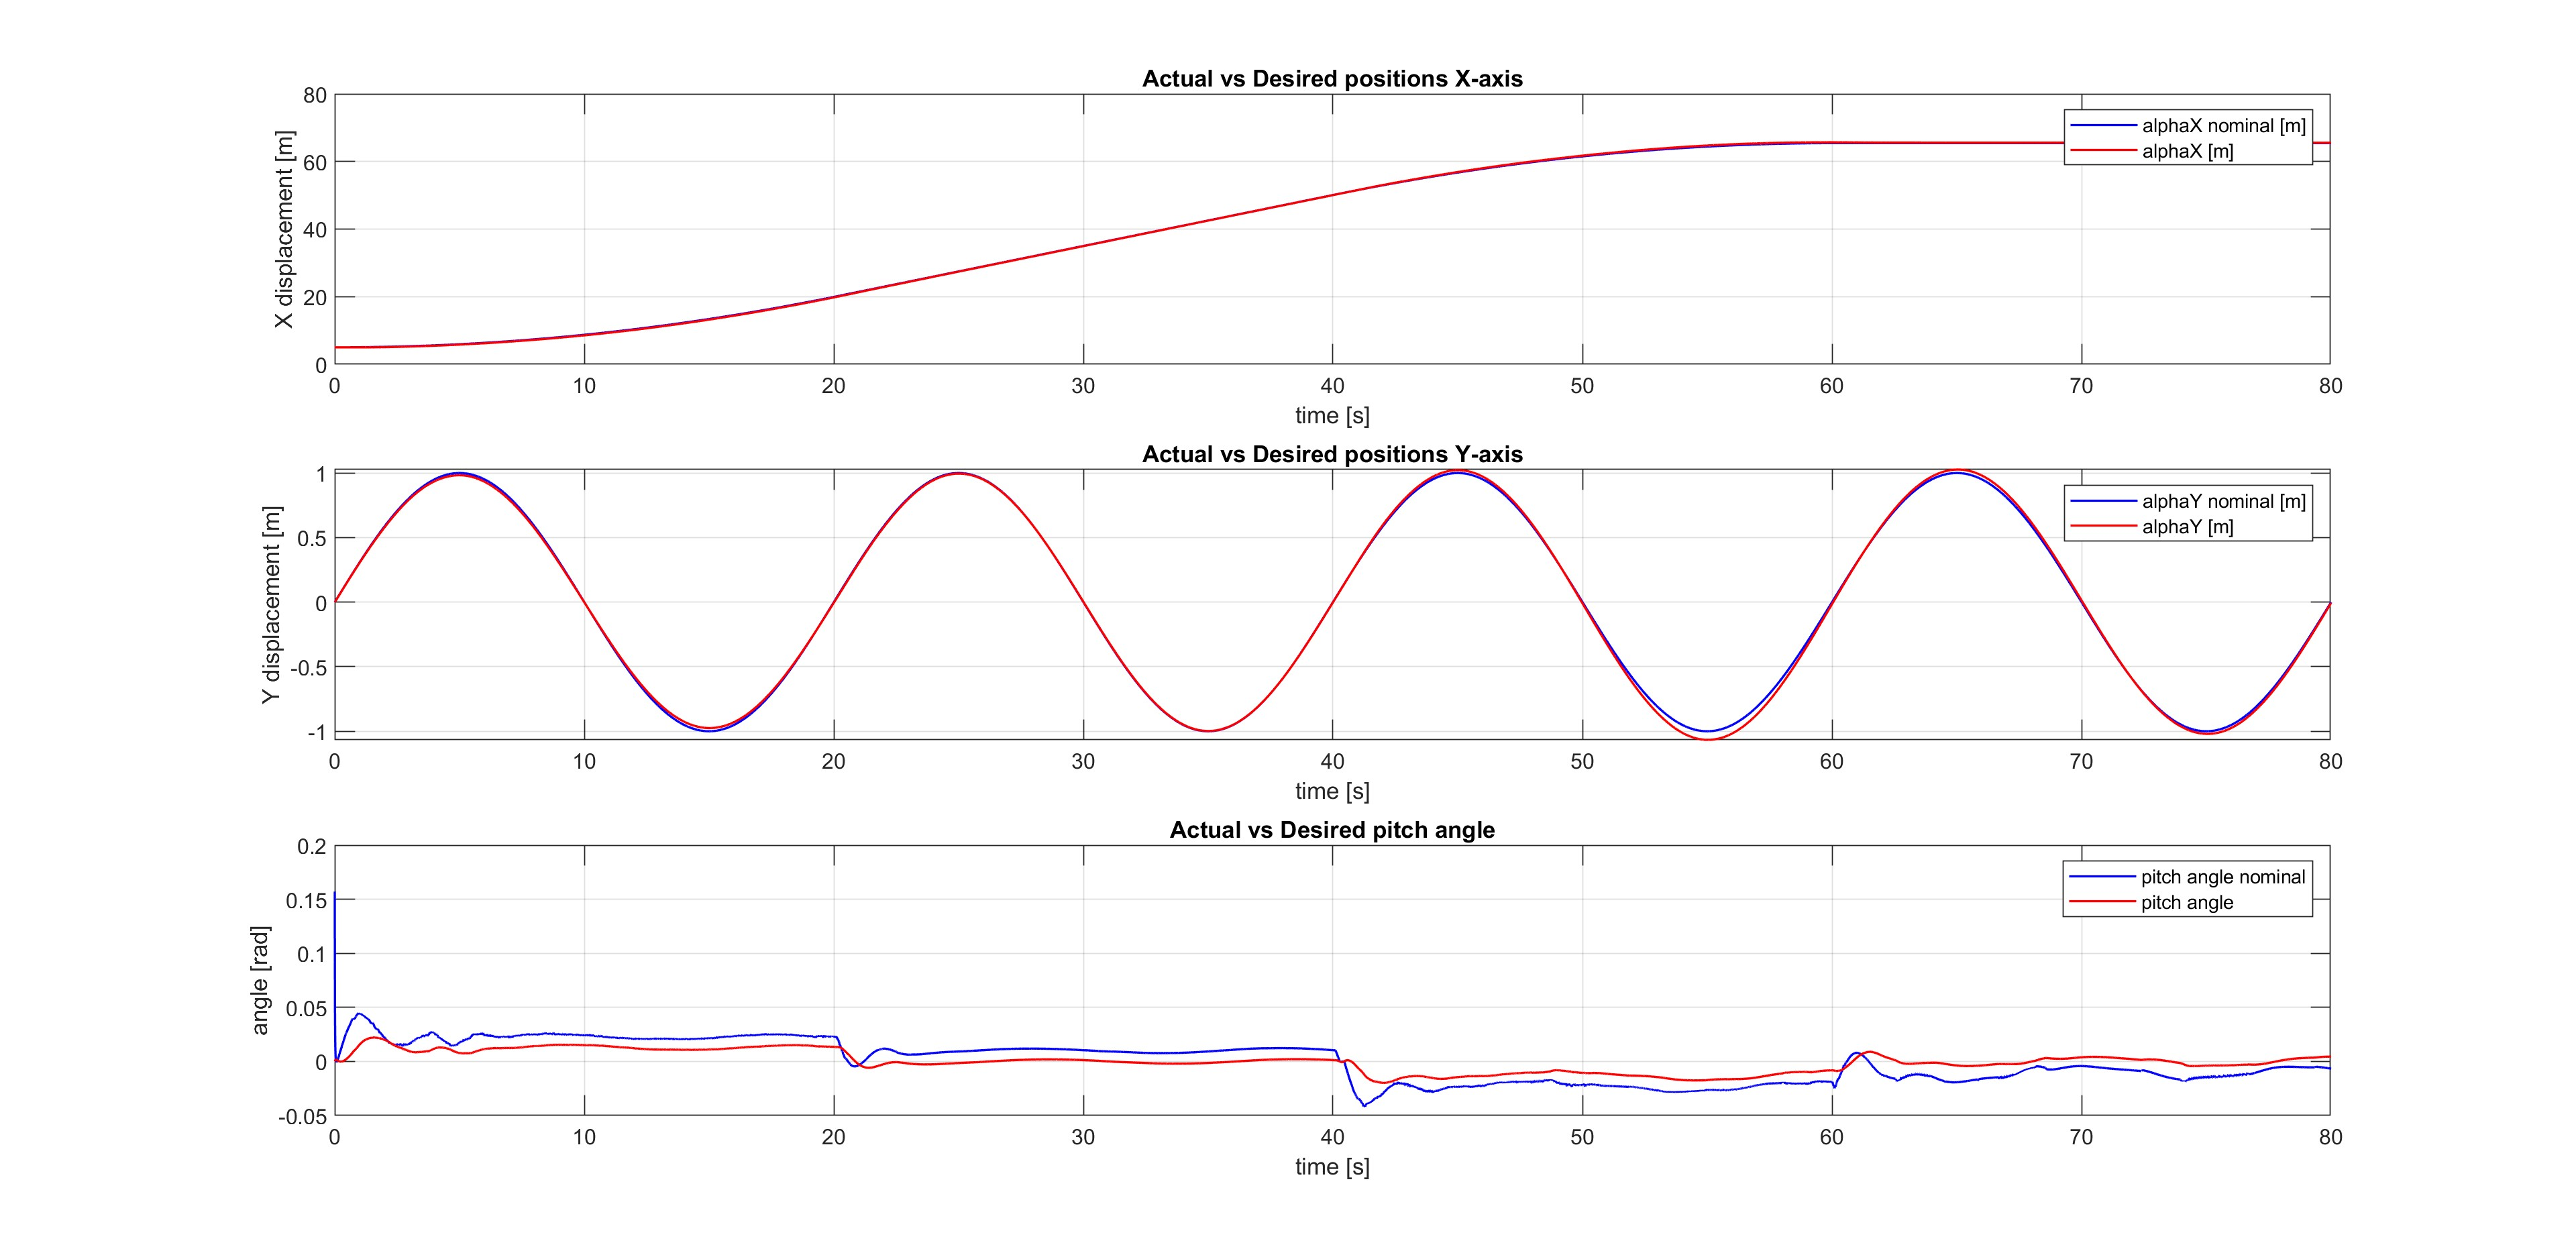
\includegraphics[width=1\linewidth]{Images/sine trajectory/Position_error.jpg}
    \caption{Sinusoidal trajectory Position error.}
    \label{fig:Sinusoidal trajectory Position error}
\end{figure}

\begin{figure}
    \centering
    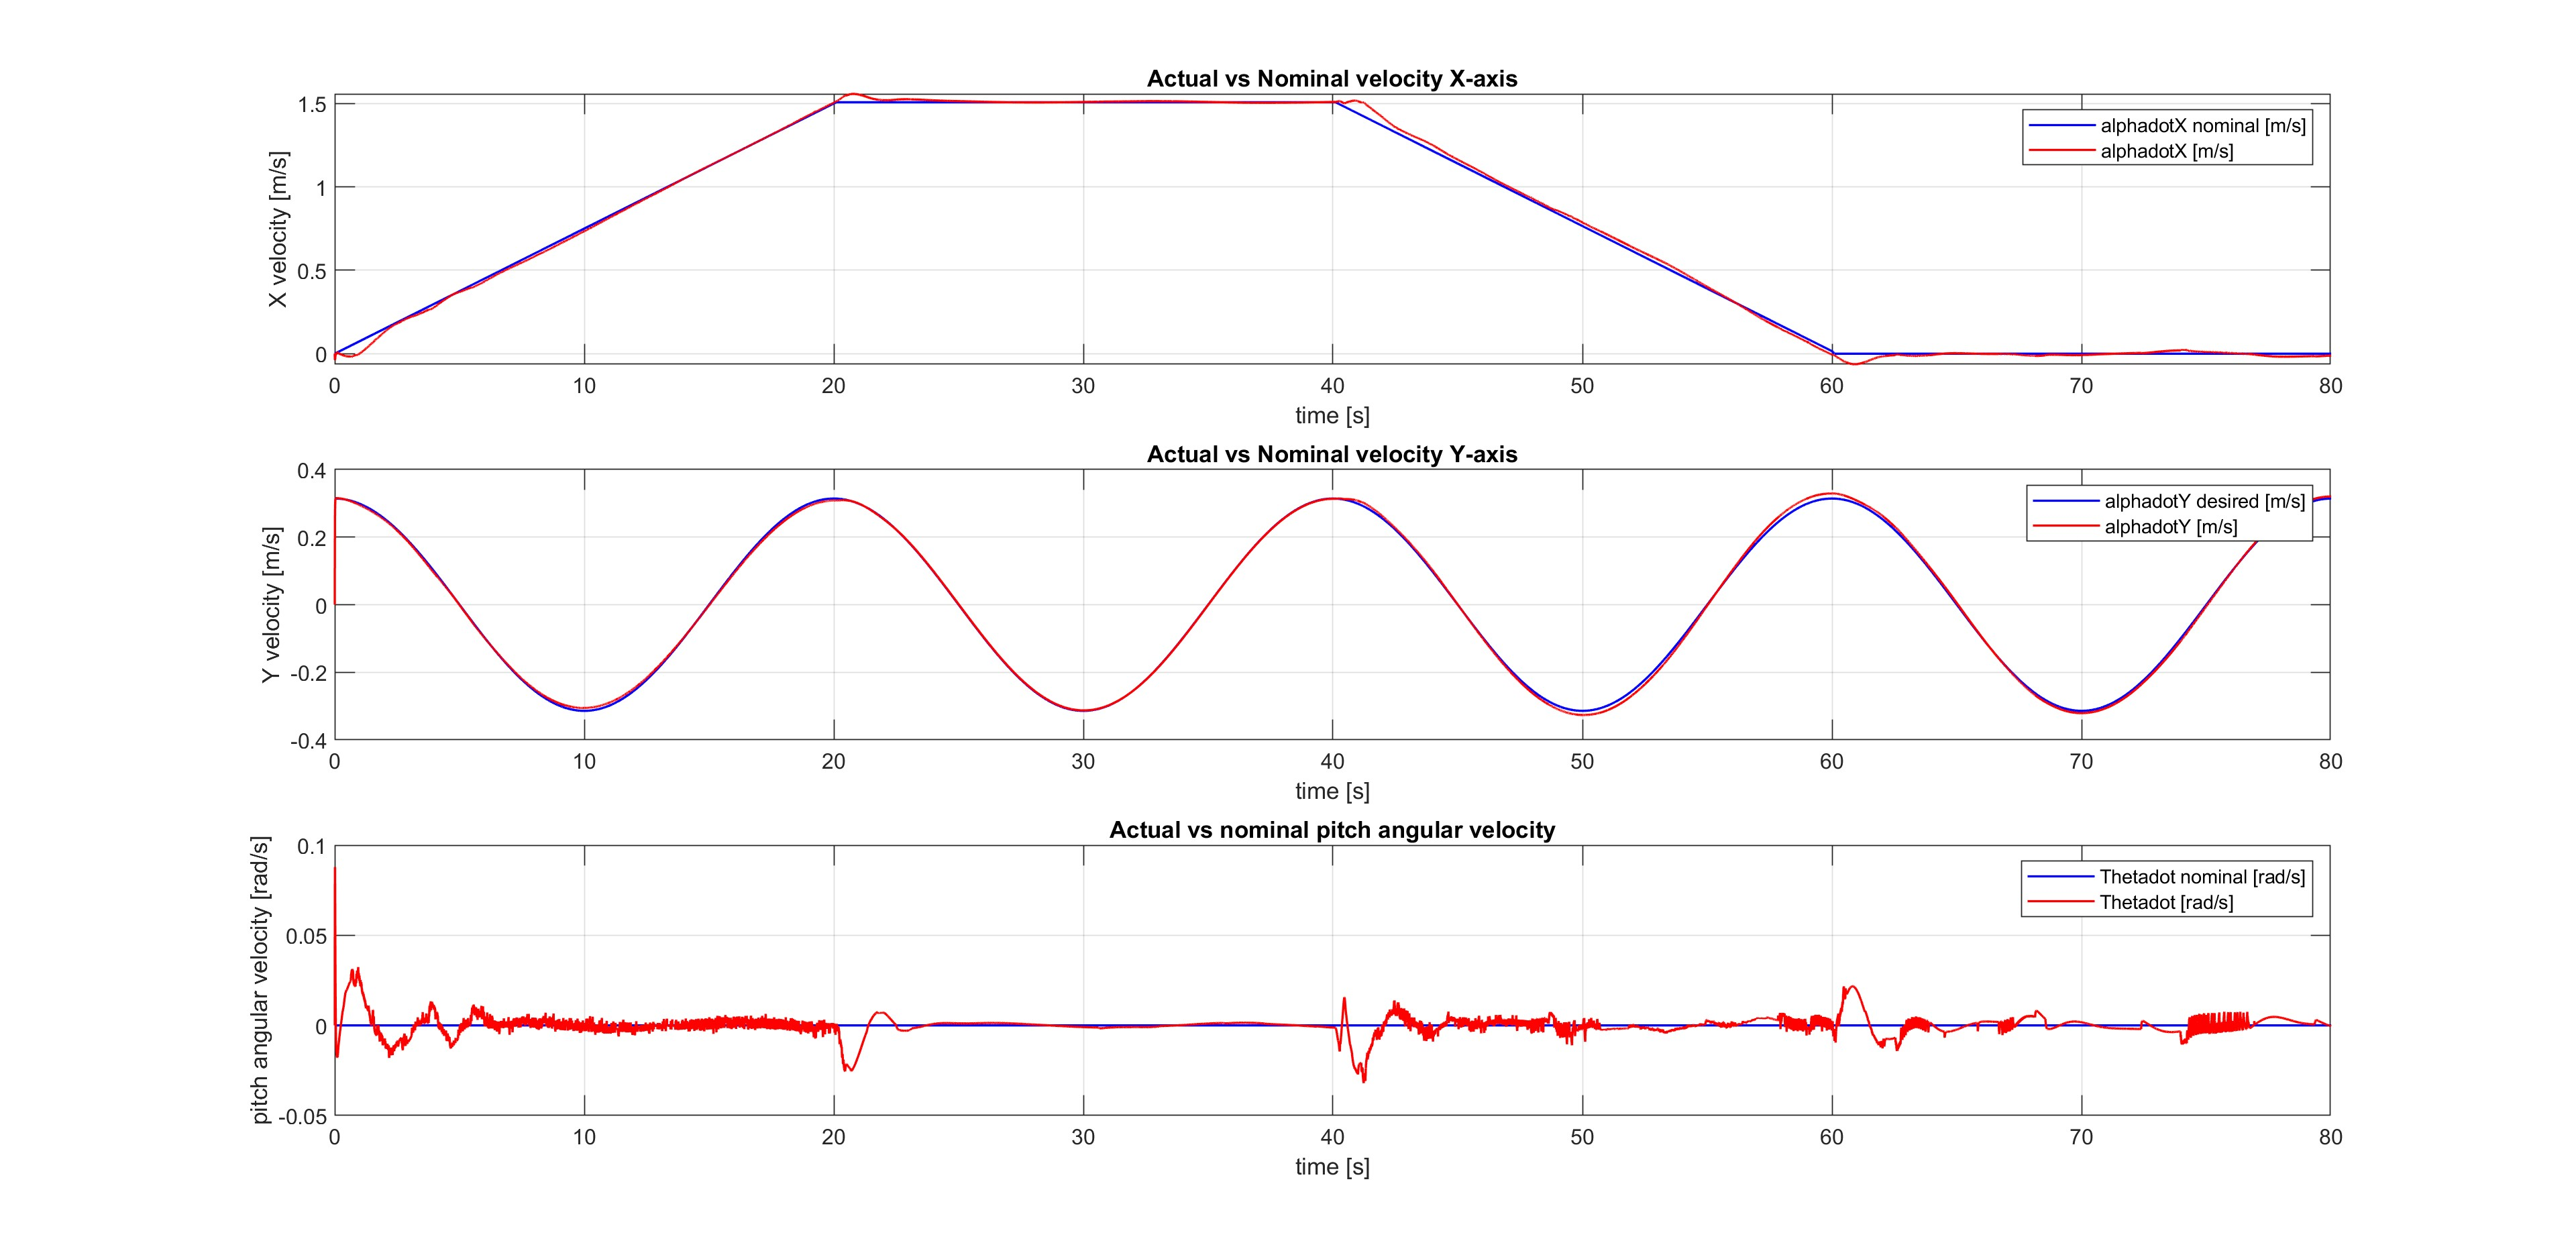
\includegraphics[width=1\linewidth]{Images/sine trajectory/Velocity_error.jpg}
    \caption{Sinusoidal trajectory Velocity error.}
    \label{fig:Sinusoidal trajectory Velocity error}
\end{figure}

Also in this last case the actual red curves follow the nominal blue ones both in position (Figure\ref{fig:Sinusoidal trajectory Position error}) and in velocity (Figure\ref{fig:Sinusoidal trajectory Velocity error}). 





\chapter{Robustness Analysis}
\label{ch:chapter_six}%
% The \label{...}% enables to remove the small indentation that is generated, always leave the % symbol.

The final part of this work involves the robustness analysis of the controller in response to changes in the model. In simulating real-world applications, our objective is to identify a set of gains and weights that ensure the stability and performance of the controller under various load conditions. This test represents the effects of loading and unloading the E-Cargo, which from the controller point of view means changing the model. It was conducted by keeping the controller parameters and the URDF file constants, while changing the robot parameters in simulation.

Considering that in the unloaded case, the trailer body weights 20 kg, the URDF file given in input represents an intermediate load condition in which the E-Cargo is loaded at half of its maximum capacity, while in the simulation we reproduce three different loading situations:

\begin{itemize}
    \item unloaded case (20 kg)
    \item half loaded case (40 kg)
    \item maximum loaded case (60 kg)
\end{itemize}

To reproduce the worse case scenario, also a disturbance on the friction coefficient has been added, meaning that in the controller we use $\mu_c = 0.4$ simulating wet asphalt, while in simulation we use $\mu_c = 0.3$ which is a limit case in most of the applications.

In all subsequent figures, red trajectories depict the actual paths, while blue trajectories represent the nominal paths.
The nominal trajectories are the same used in \cref{sec:Simulation results}, and the controller parameters are the same defined in Table \ref{tab:Set of Gains and Weights}.

\section{Swing-up with model uncertainties}
\label{sec:Swing-up with model uncertainties}

Following the same outline of \cref{sec:Simulation results}, we start from the Swing-up test, which is the most critical one in case of model uncertainties, and then test the tracking of a generic sinusoidal trajectory in the plane.

\subsection{Swing-up in the unloaded case}
\label{subsec:Swing-up in the unloaded case}

\begin{figure}
    \centering
    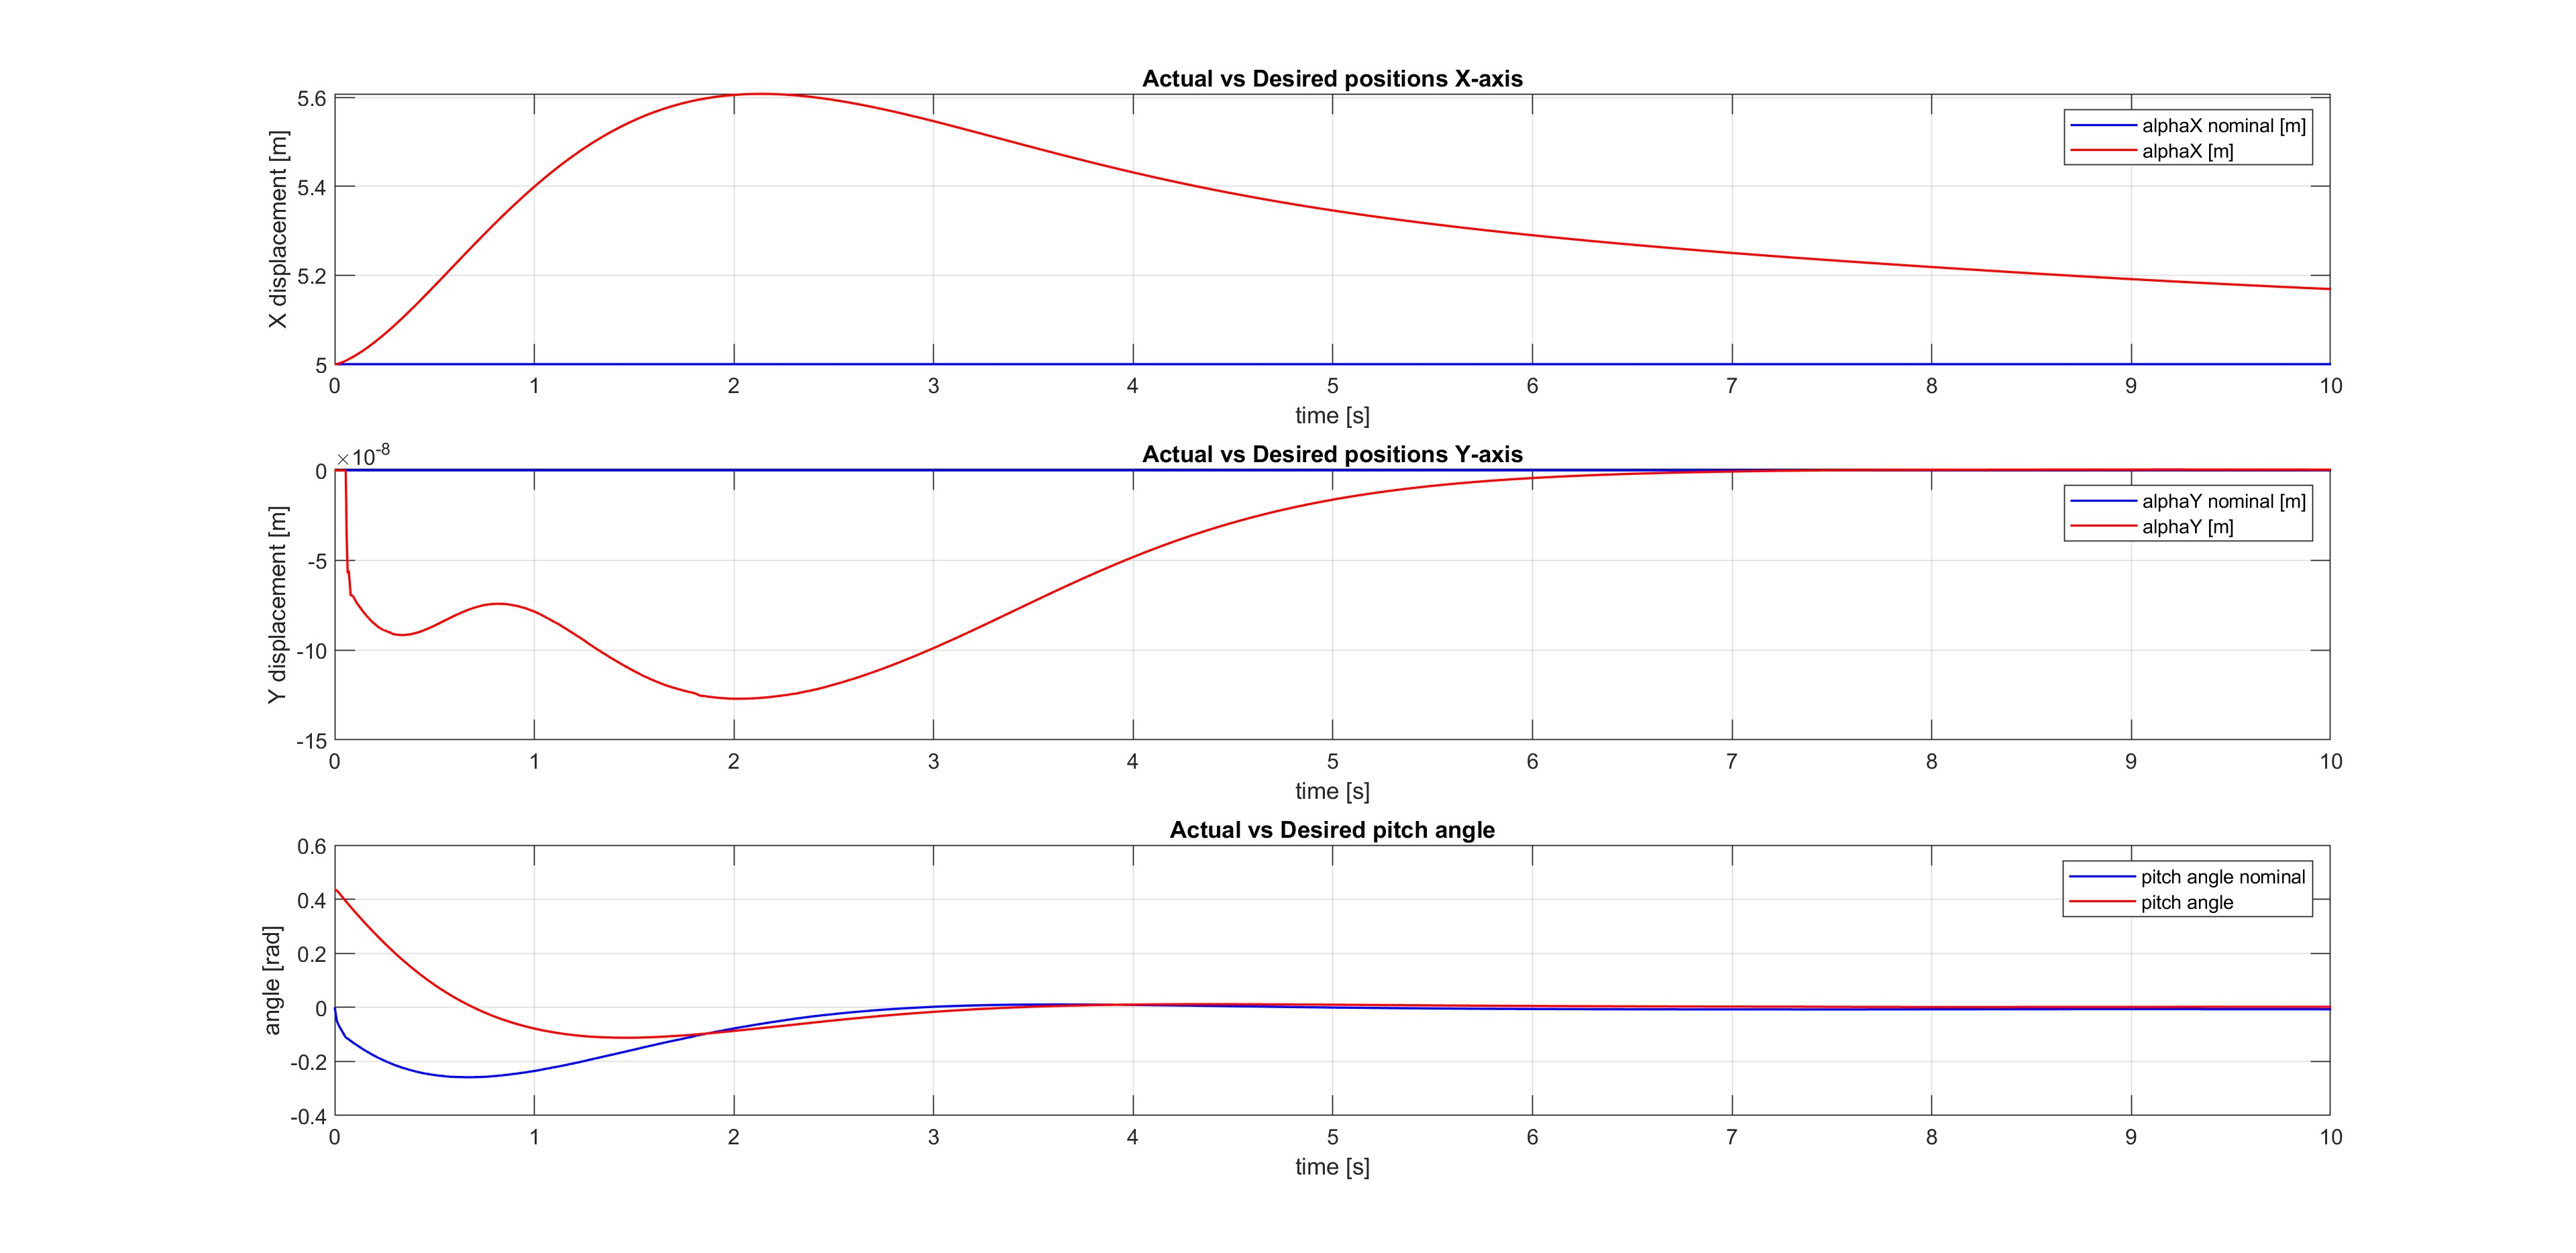
\includegraphics[width=1\linewidth]{Images/Robustness analysis/Unloaded/Swing-Up/Position_error.jpg}
    \caption{Swing-up position error with disturbances in the unloaded case.}
    \label{fig:Swing-up position error with disturbances in the unloaded case}
\end{figure}

\begin{figure}
    \centering
    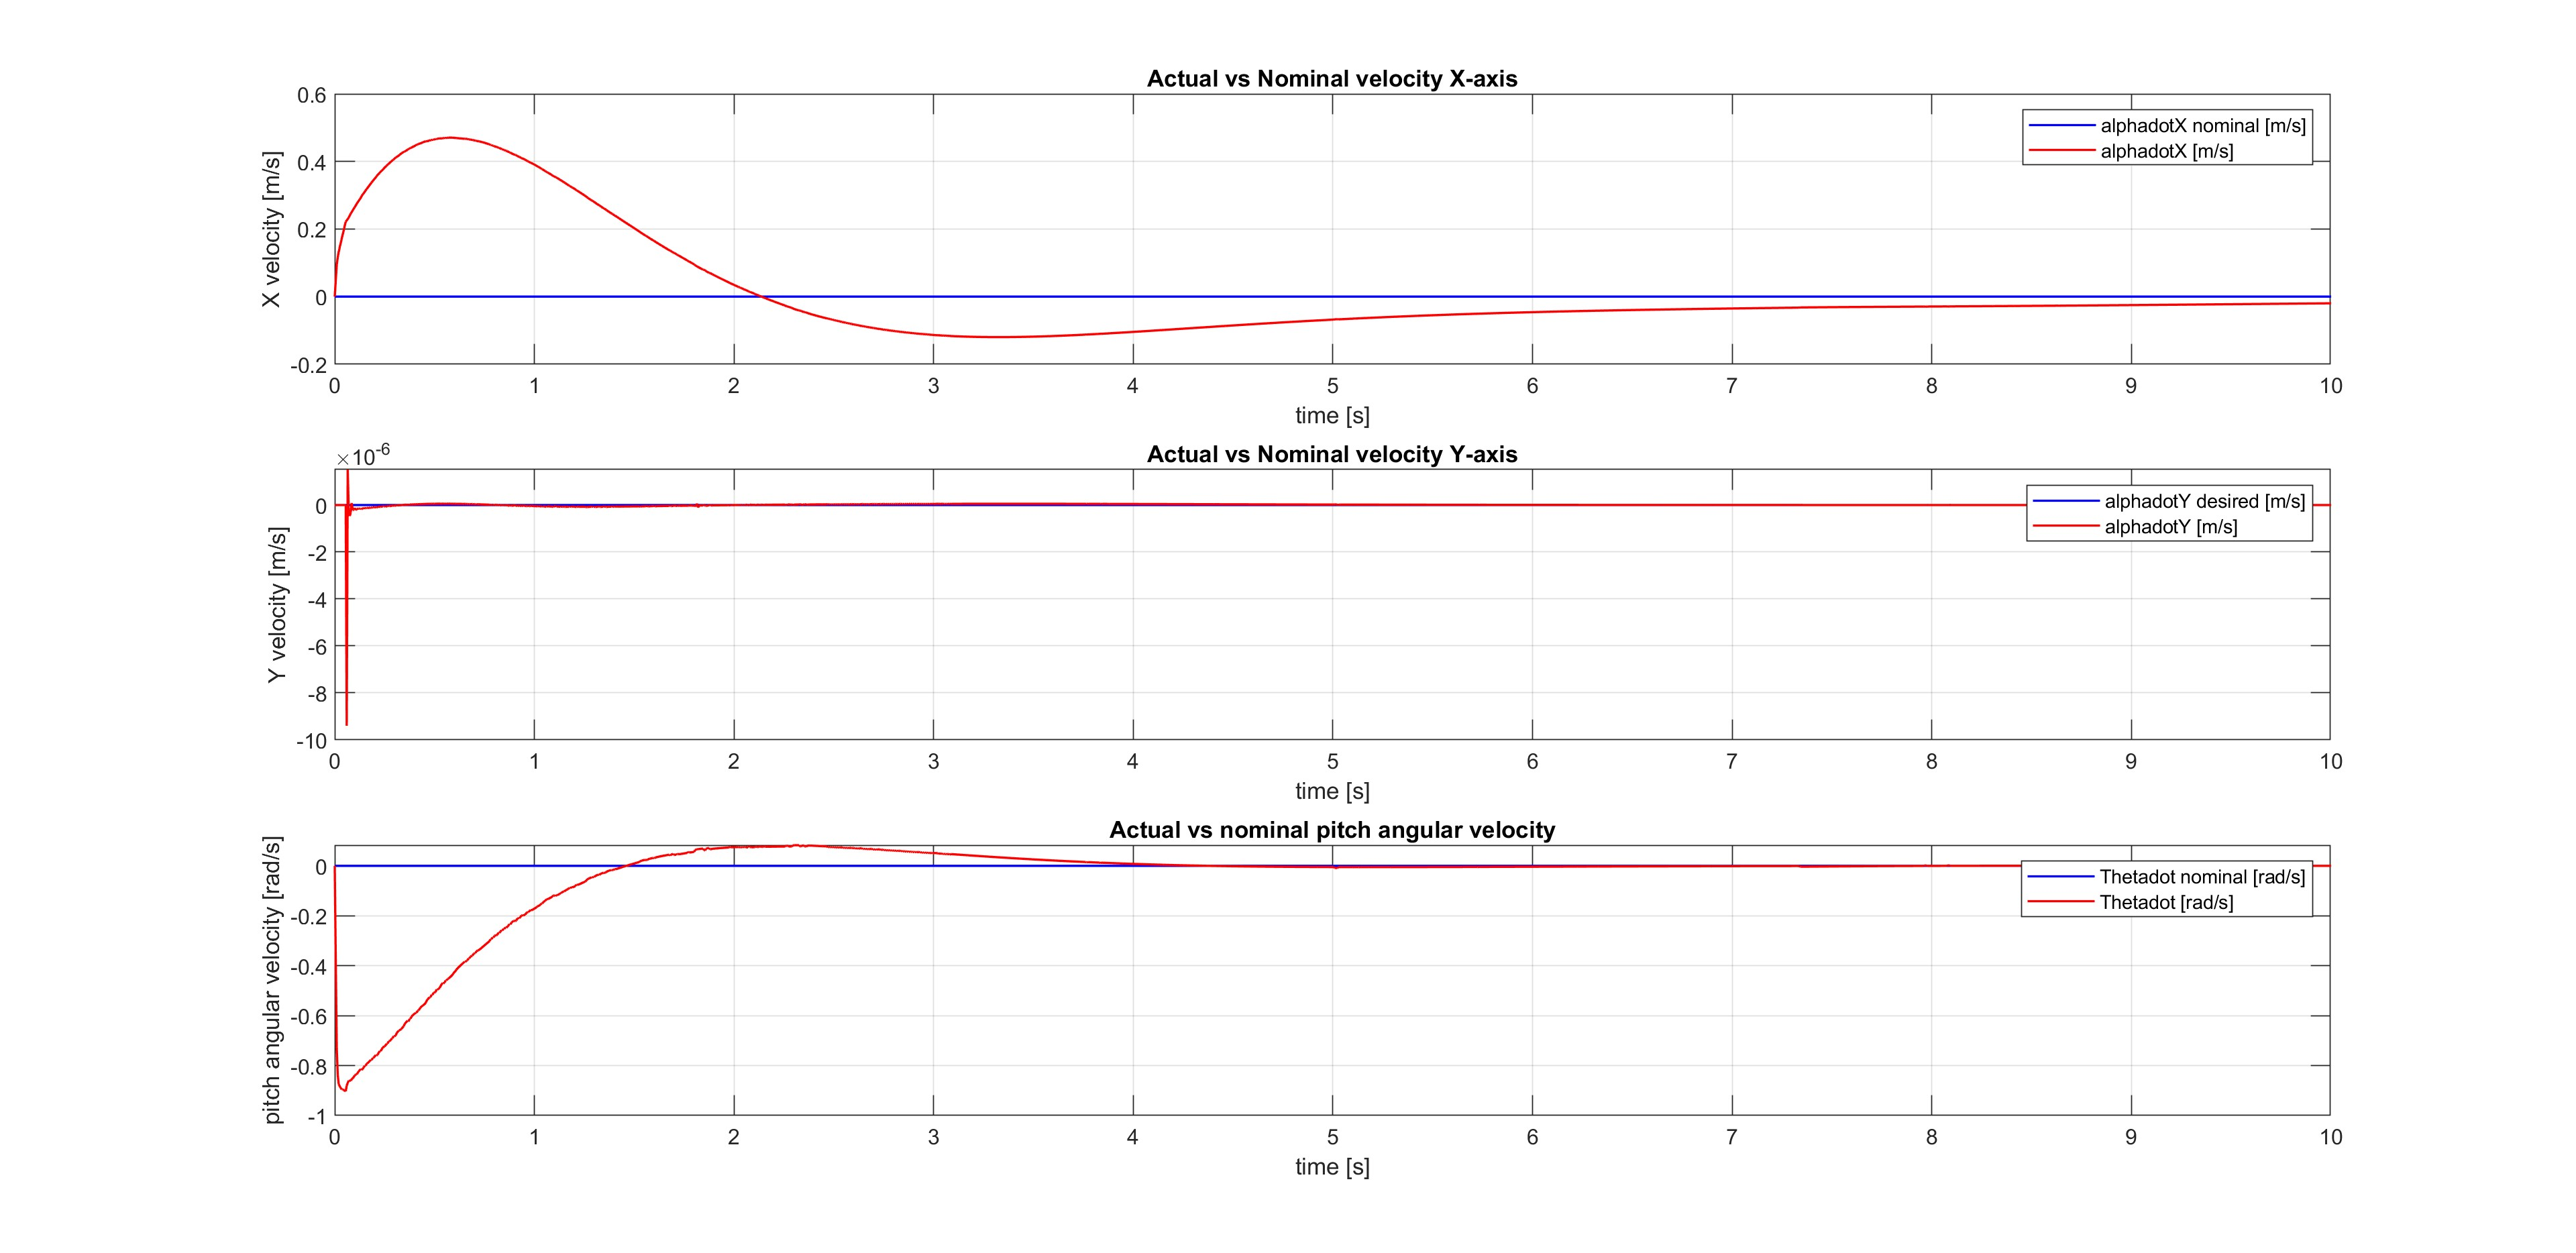
\includegraphics[width=1\linewidth]{Images/Robustness analysis/Unloaded/Swing-Up/Velocity_error.jpg}
    \caption{Swing-up velocity error with disturbances in the unloaded case.}
    \label{fig:Swing-up velocity error with disturbances in the unloaded case}
\end{figure}

Figures \ref{fig:Swing-up position error with disturbances in the unloaded case} and \ref{fig:Swing-up velocity error with disturbances in the unloaded case}, show the nominal and actual trajectories in position and velocity respectively for the unloaded condition, and it can be noticed how, after the transient, the actual trajectories approach the nominal ones.

Figure \ref{fig:Swing-up slipping velocity with disturbances in the unloaded case} instead shows in red the slipping velocity between the wheels and the terrain, and in green the solver status which is defined as follows: 

\begin{itemize}
    \item 1 = Solved
    \item 2 = Solved with higher tolerance
    \item -2 = maximum number of iterations reached
\end{itemize}

\begin{figure}
    \centering
    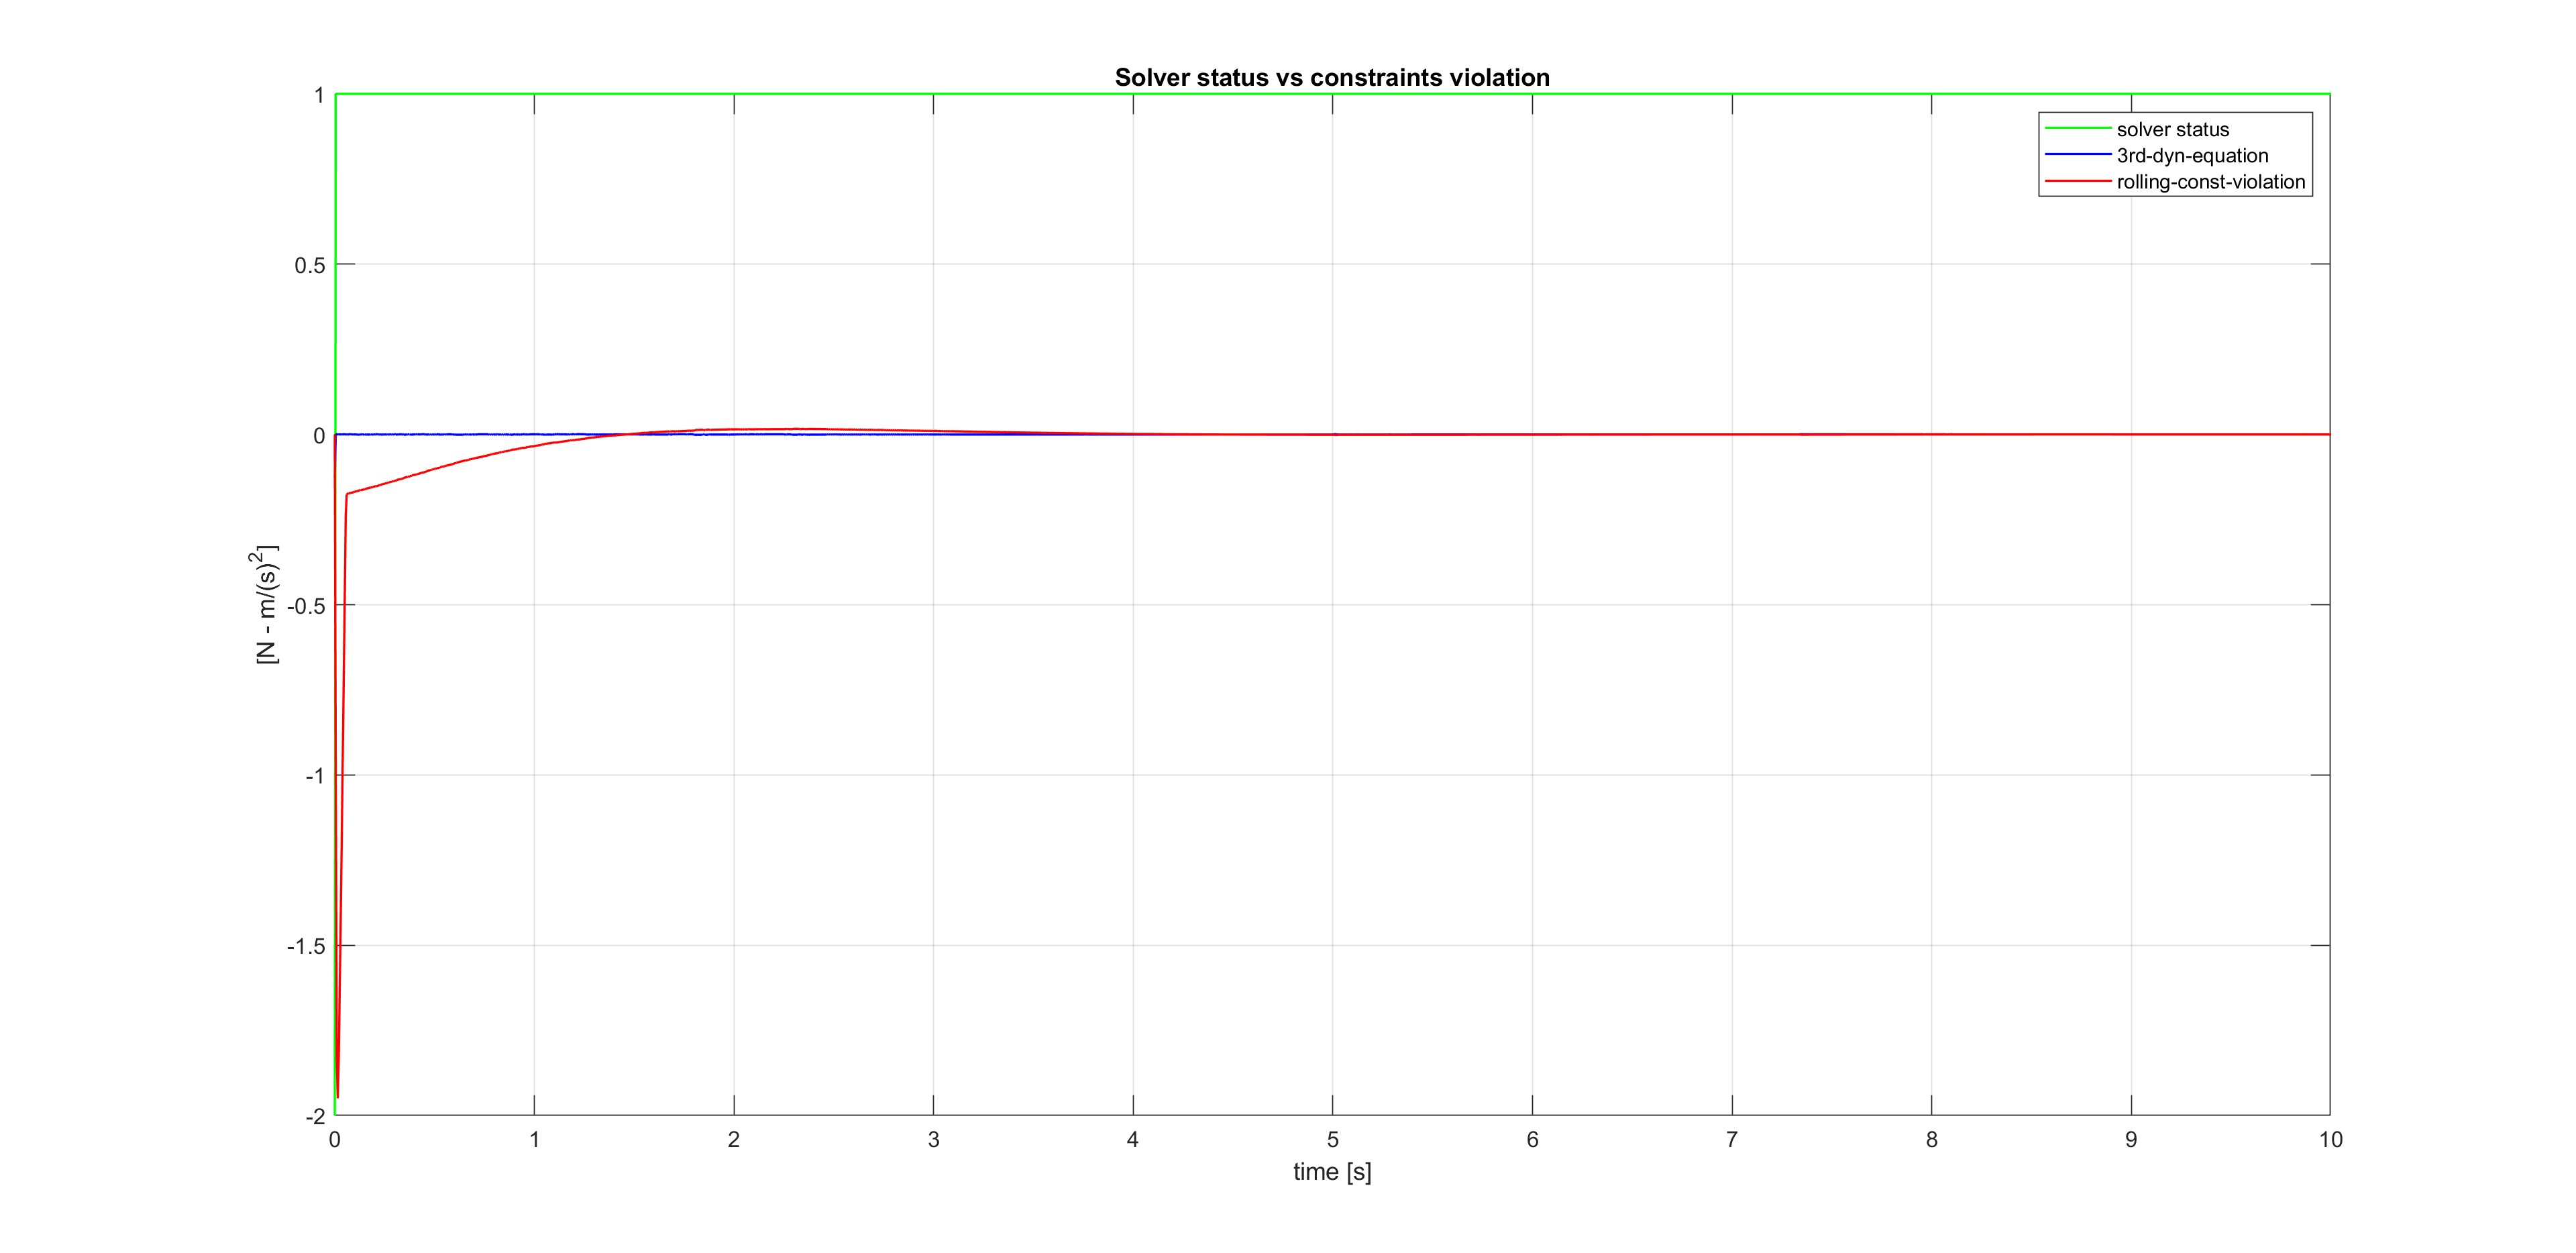
\includegraphics[width=1\linewidth]{Images/Robustness analysis/Unloaded/Swing-Up/Slipping_velocity.jpg}
    \caption{Swing-up slipping velocity with disturbances in the unloaded case.}
    \label{fig:Swing-up slipping velocity with disturbances in the unloaded case}
\end{figure}

\subsection{Swing-up in the case of half load}
\label{subsec:Swing-up in the case of half load}

\begin{figure}
    \centering
    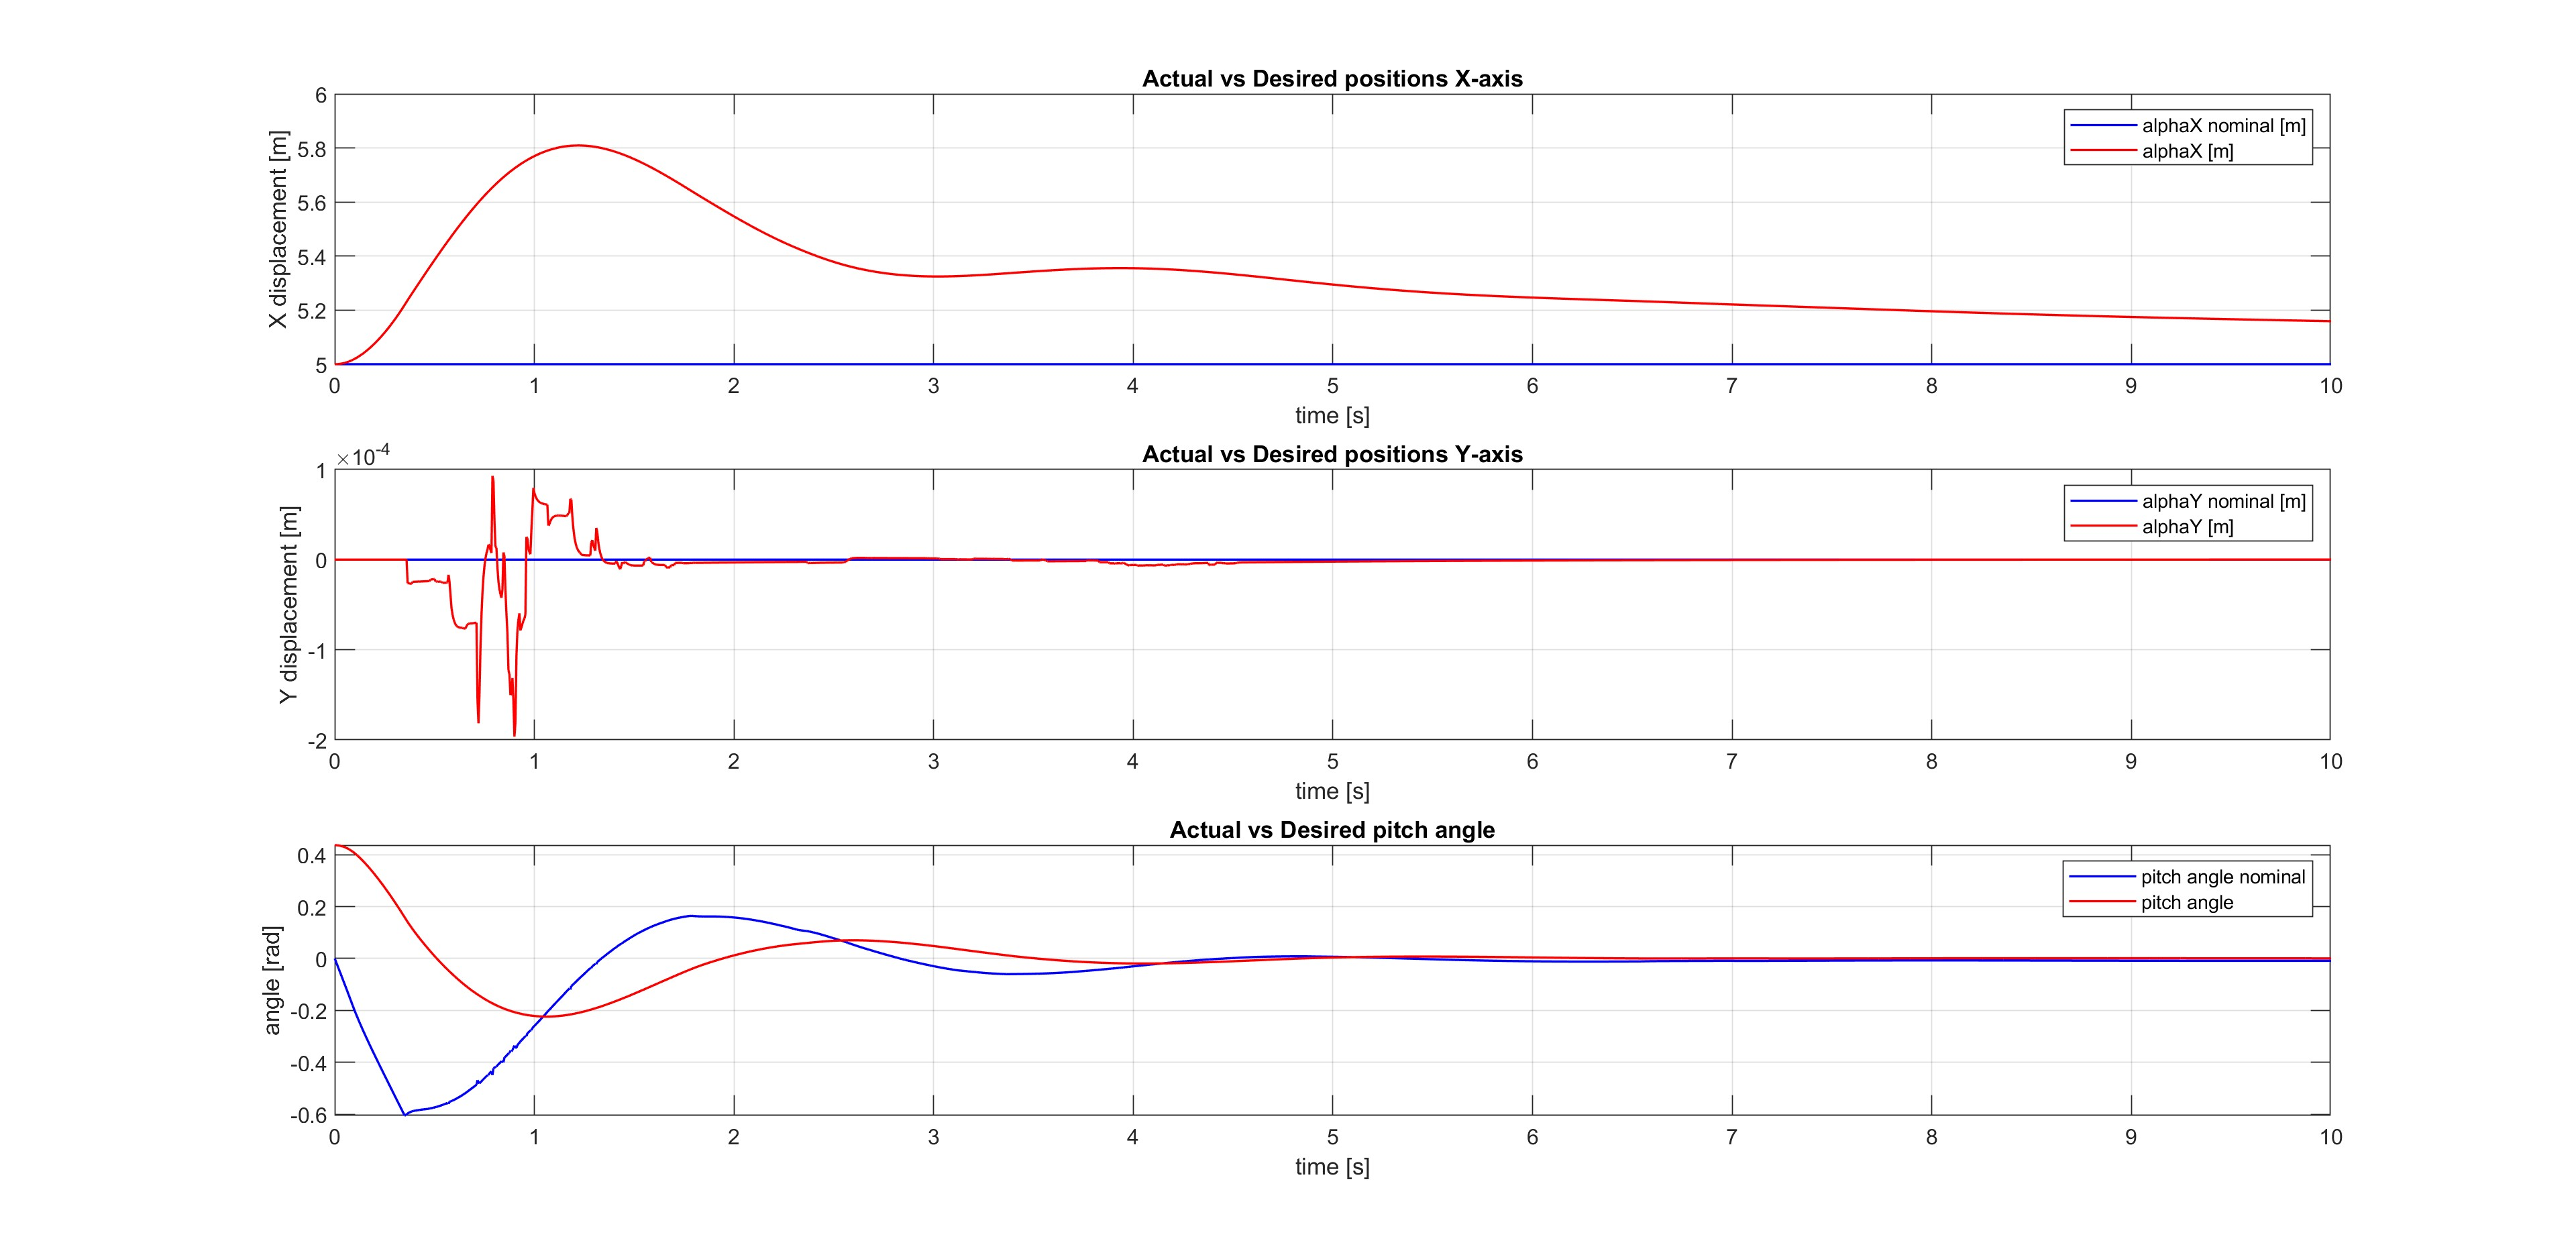
\includegraphics[width=1\linewidth]{Images/Robustness analysis/intermediate load/Swing-Up/Position_error.jpg}
    \caption{Swing-up position error with disturbances in the case of half load.}
    \label{fig:Swing-up position error with disturbances in the case of half load}
\end{figure}

\begin{figure}
    \centering
    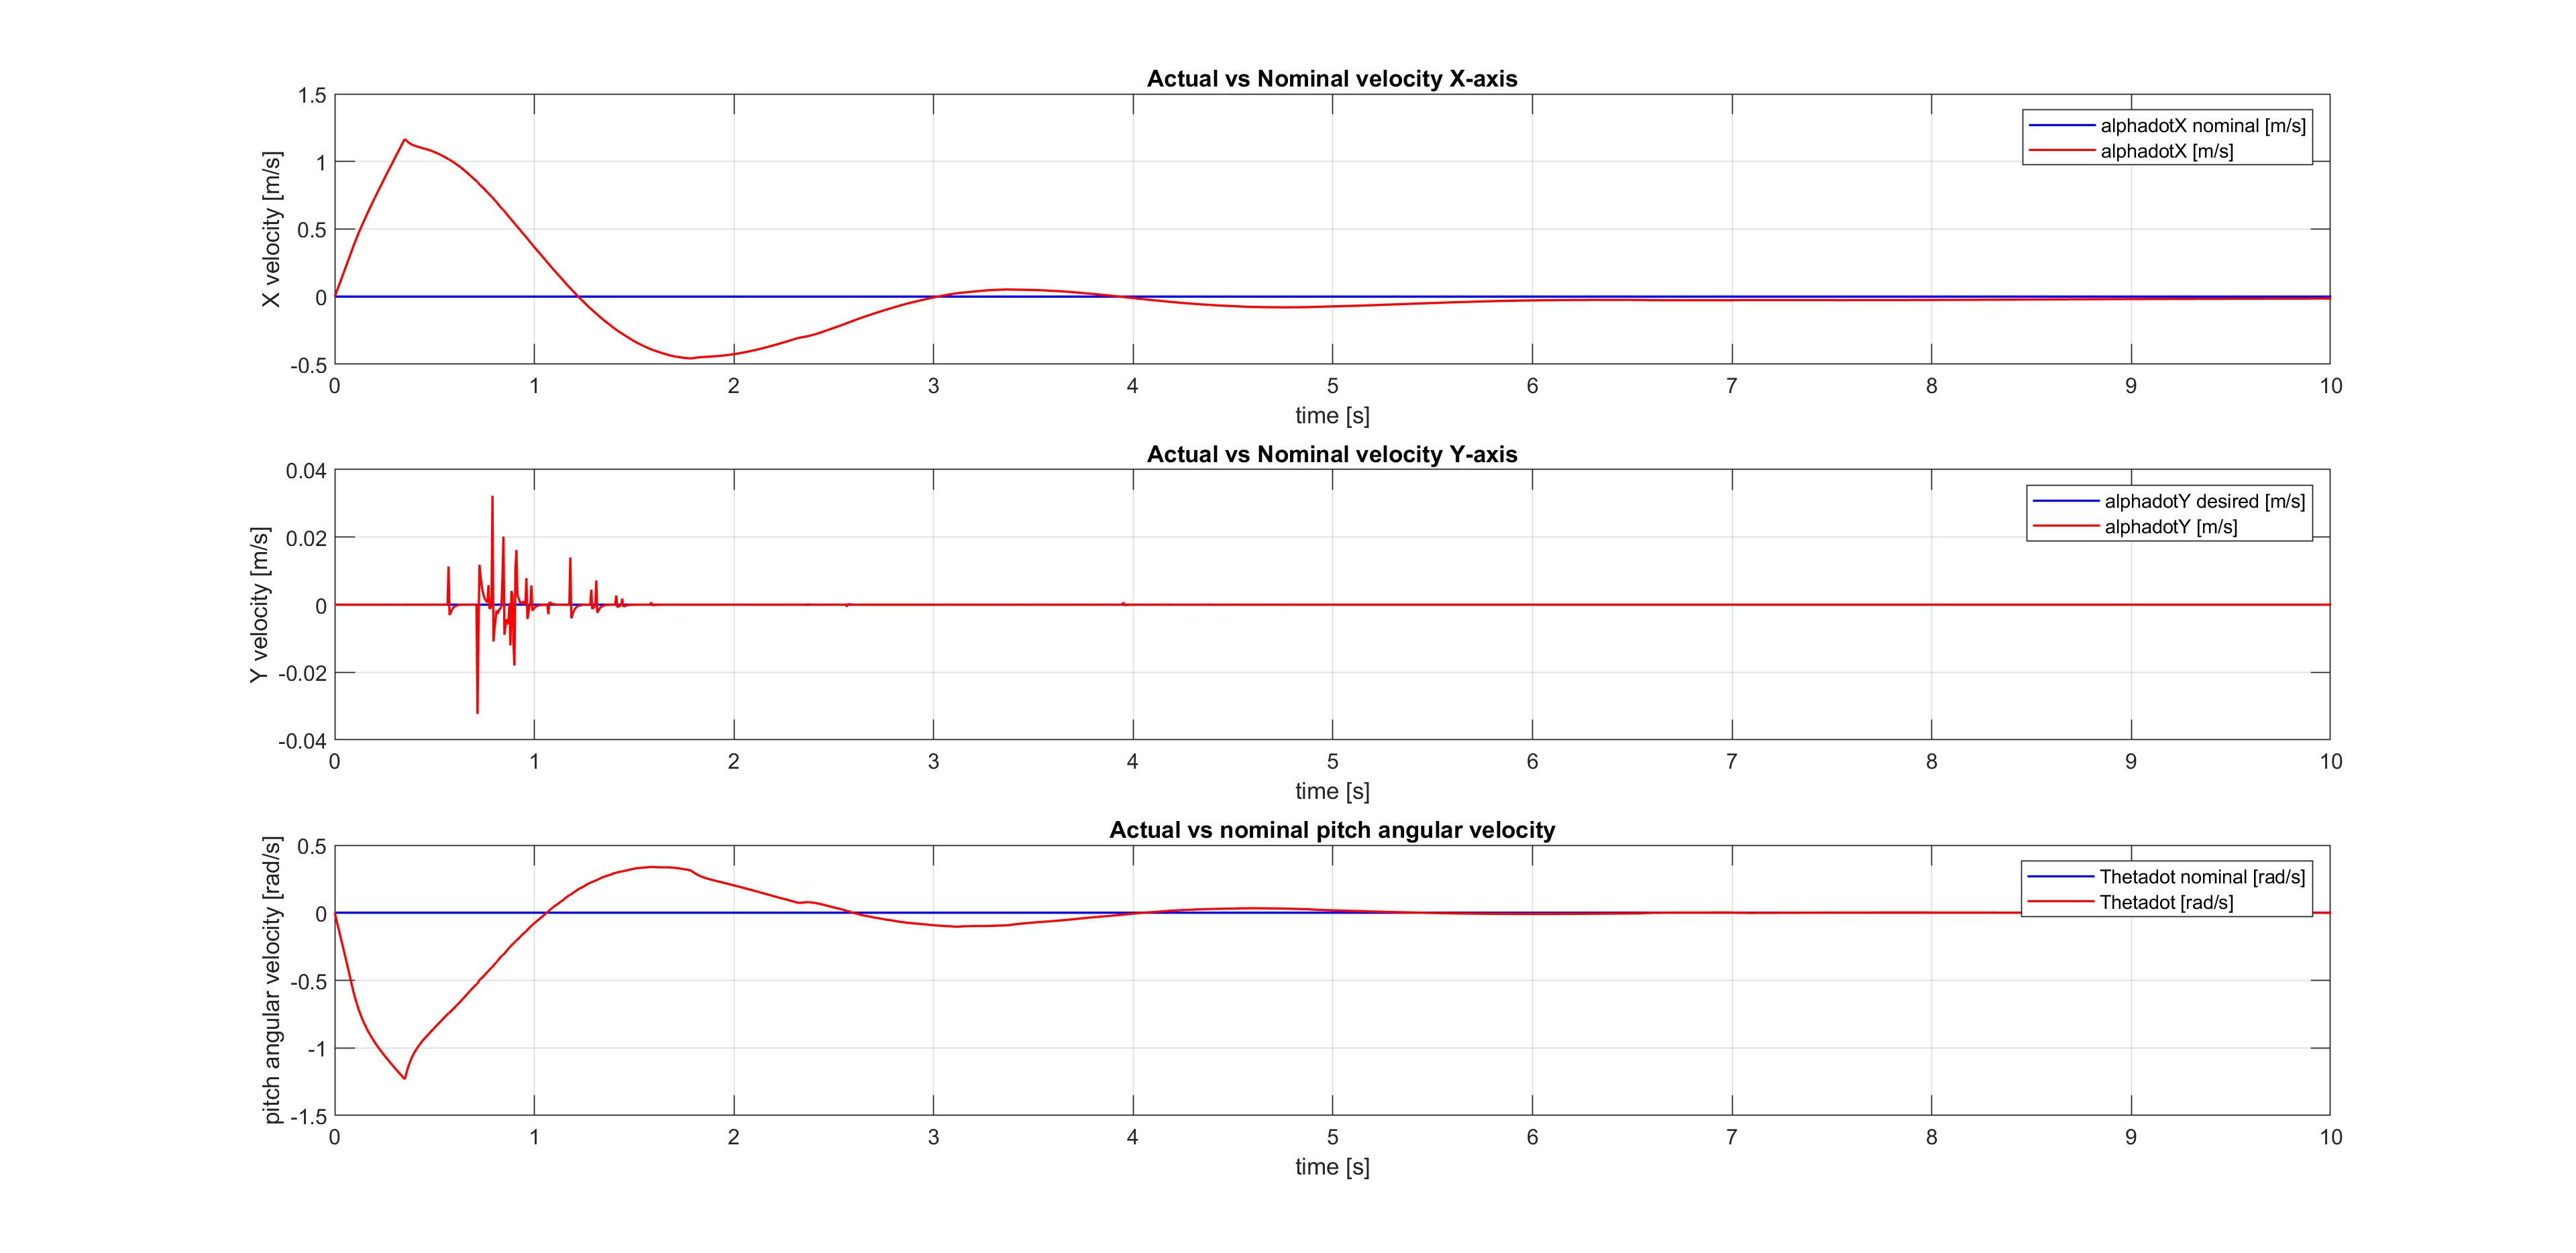
\includegraphics[width=1\linewidth]{Images/Robustness analysis/intermediate load/Swing-Up/Velocity_error.jpg}
    \caption{Swing-up velocity error with disturbances in the case of half load.}
    \label{fig:Swing-up velocity error with disturbances in the case of half load}
\end{figure}

Figures \ref{fig:Swing-up position error with disturbances in the case of half load} and \ref{fig:Swing-up velocity error with disturbances in the case of half load}, show the nominal and actual trajectories in position and velocity respectively for the condition of half load, and also in this case, after the transient, the actual trajectories approach the nominal ones.
In this situation there is a perfect match regarding the controller model and the simulator one, apart for the friction coefficient.

\begin{figure}
    \centering
    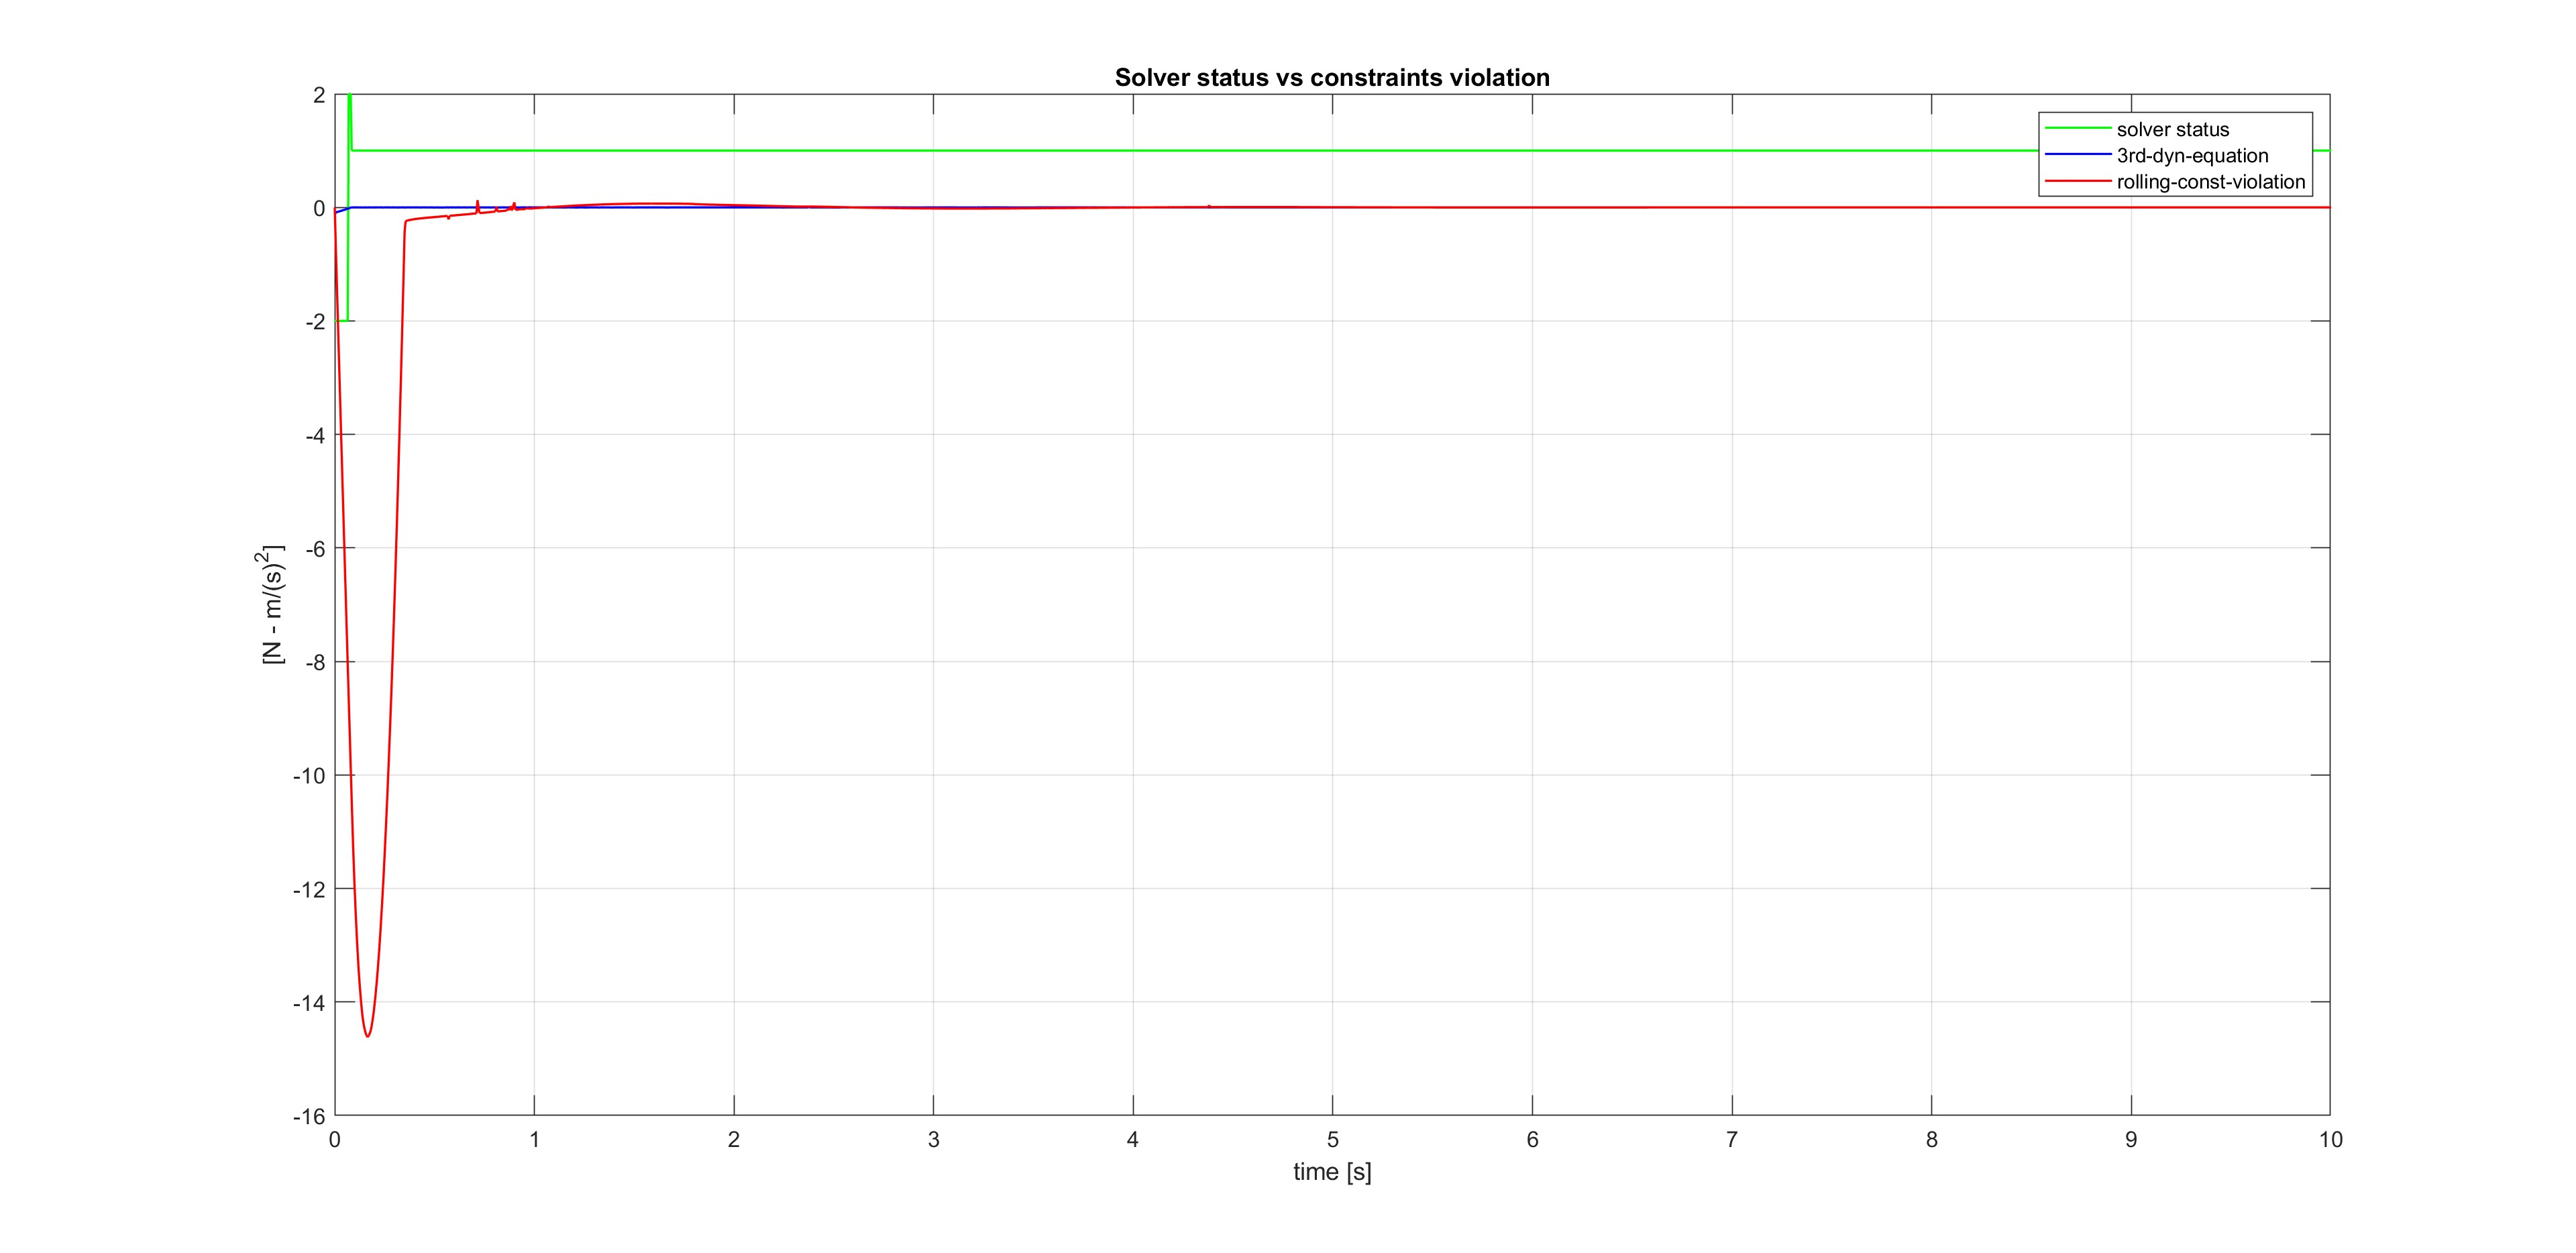
\includegraphics[width=1\linewidth]{Images/Robustness analysis/intermediate load/Swing-Up/Slipping_velocity.jpg}
    \caption{Swing-up slipping velocity with disturbances in the case of half load.}
    \label{fig:Swing-up slipping velocity with disturbances in the case of half load}
\end{figure}

In Figure \ref{fig:Swing-up slipping velocity with disturbances in the case of half load} is represented in red the slipping velocity, and in green the solver status.

\subsection{Swing-up in the case of maximum load}
\label{subsec:Swing-up in the case of maximum load}

\begin{figure}
    \centering
    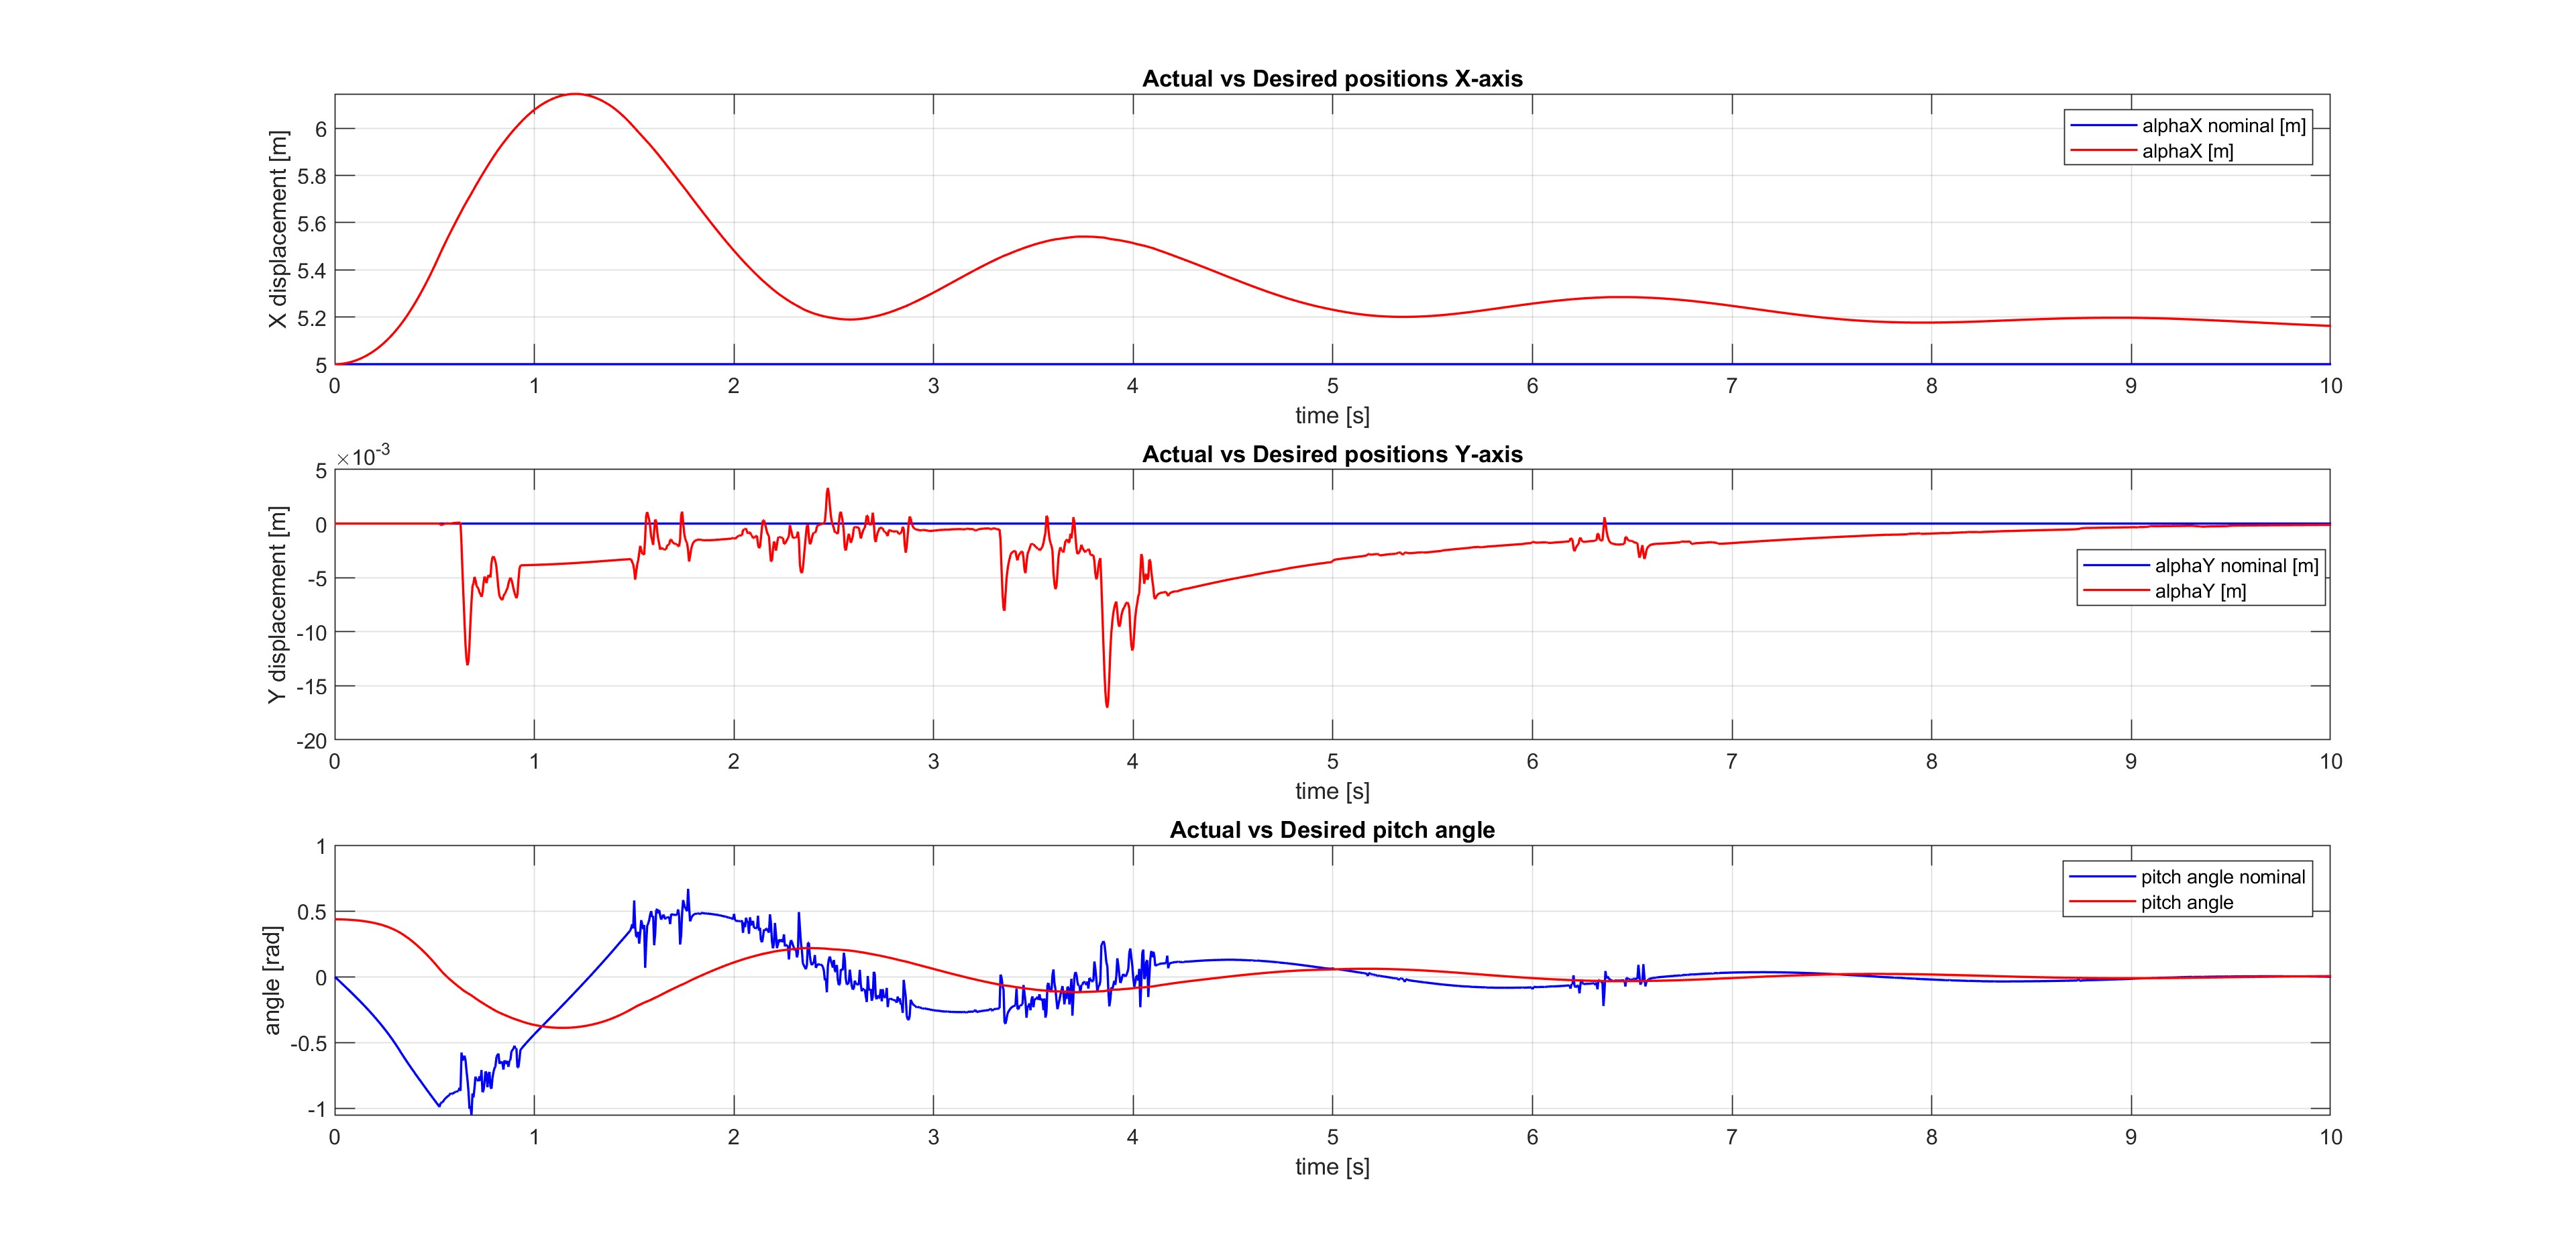
\includegraphics[width=1\linewidth]{Images/Robustness analysis/maximum load/Swing-Up/Position_error.jpg}
    \caption{Swing-up position error with disturbances in the case of maximum load.}
    \label{fig:Swing-up position error with disturbances in the case of maximum load}
\end{figure}

\begin{figure}
    \centering
    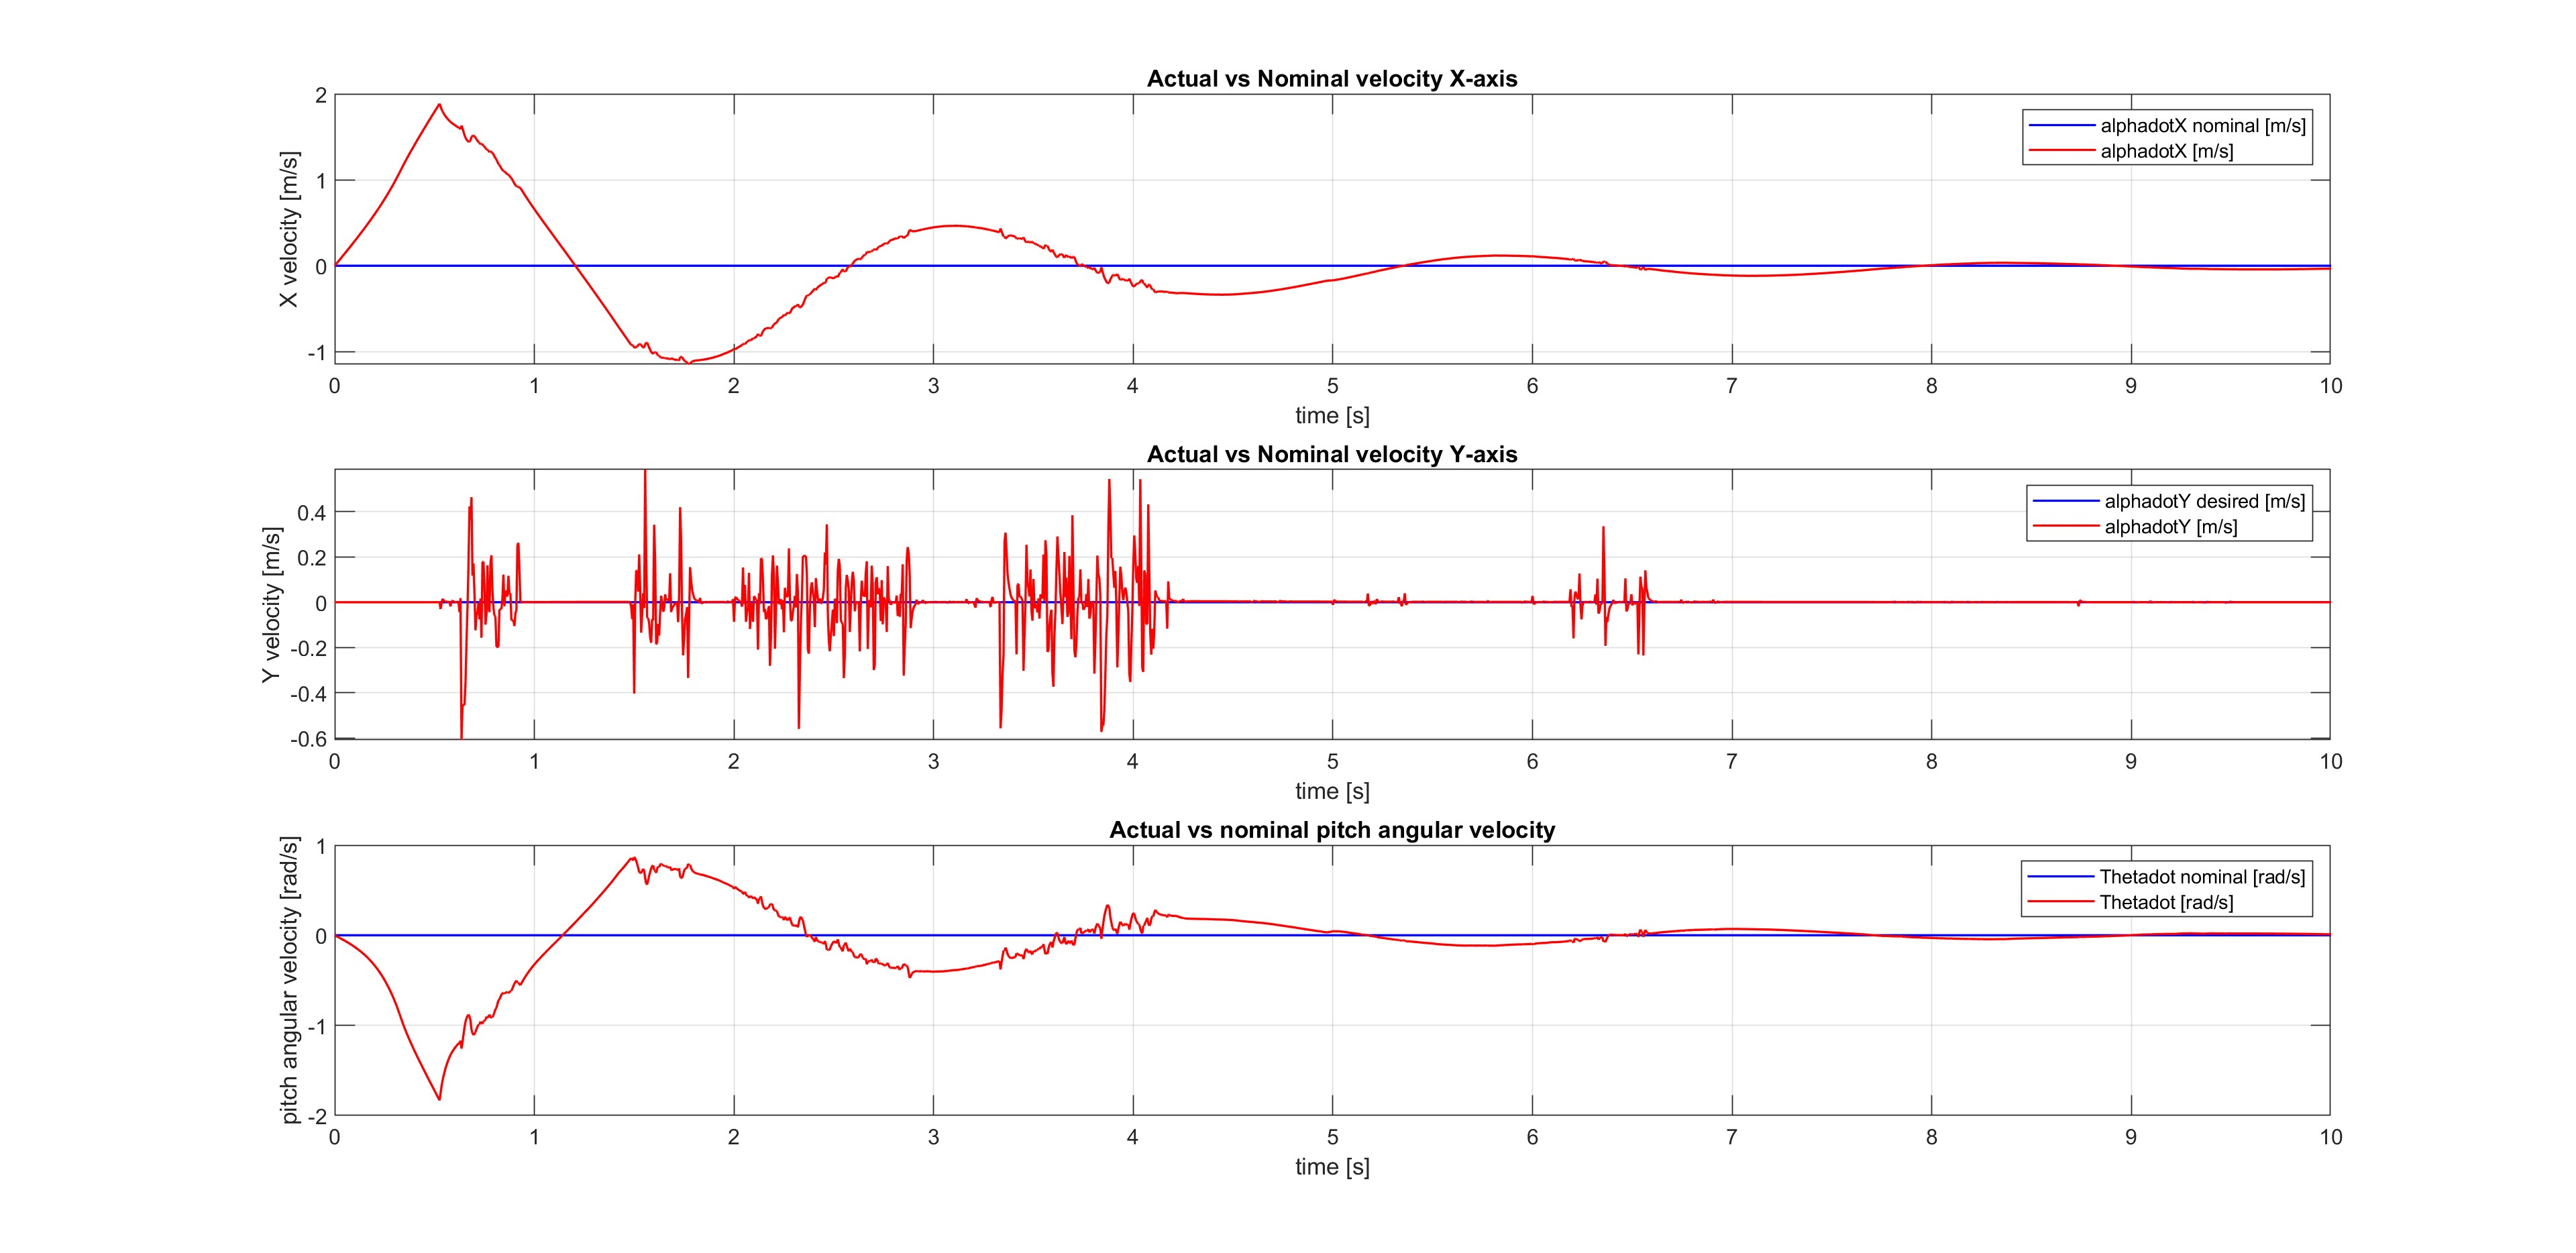
\includegraphics[width=1\linewidth]{Images/Robustness analysis/maximum load/Swing-Up/Velocity_error.jpg}
    \caption{Swing-up velocity error with disturbances in the case of maximum load.}
    \label{fig:Swing-up velocity error with disturbances in the case of maximum load}
\end{figure}

Figures \ref{fig:Swing-up position error with disturbances in the case of maximum load} and \ref{fig:Swing-up velocity error with disturbances in the case of maximum load}, show the nominal and actual trajectories in position and velocity respectively for the extreme condition of maximum load, and also in this case, the pitch angle $\theta$ is stabilized after 5 seconds.
This simulation represents the worse possible case, in the sense that the pitch starting angle is the maximum possible, the same holds for the load, and the friction coefficient is very low.   

\begin{figure}
    \centering
    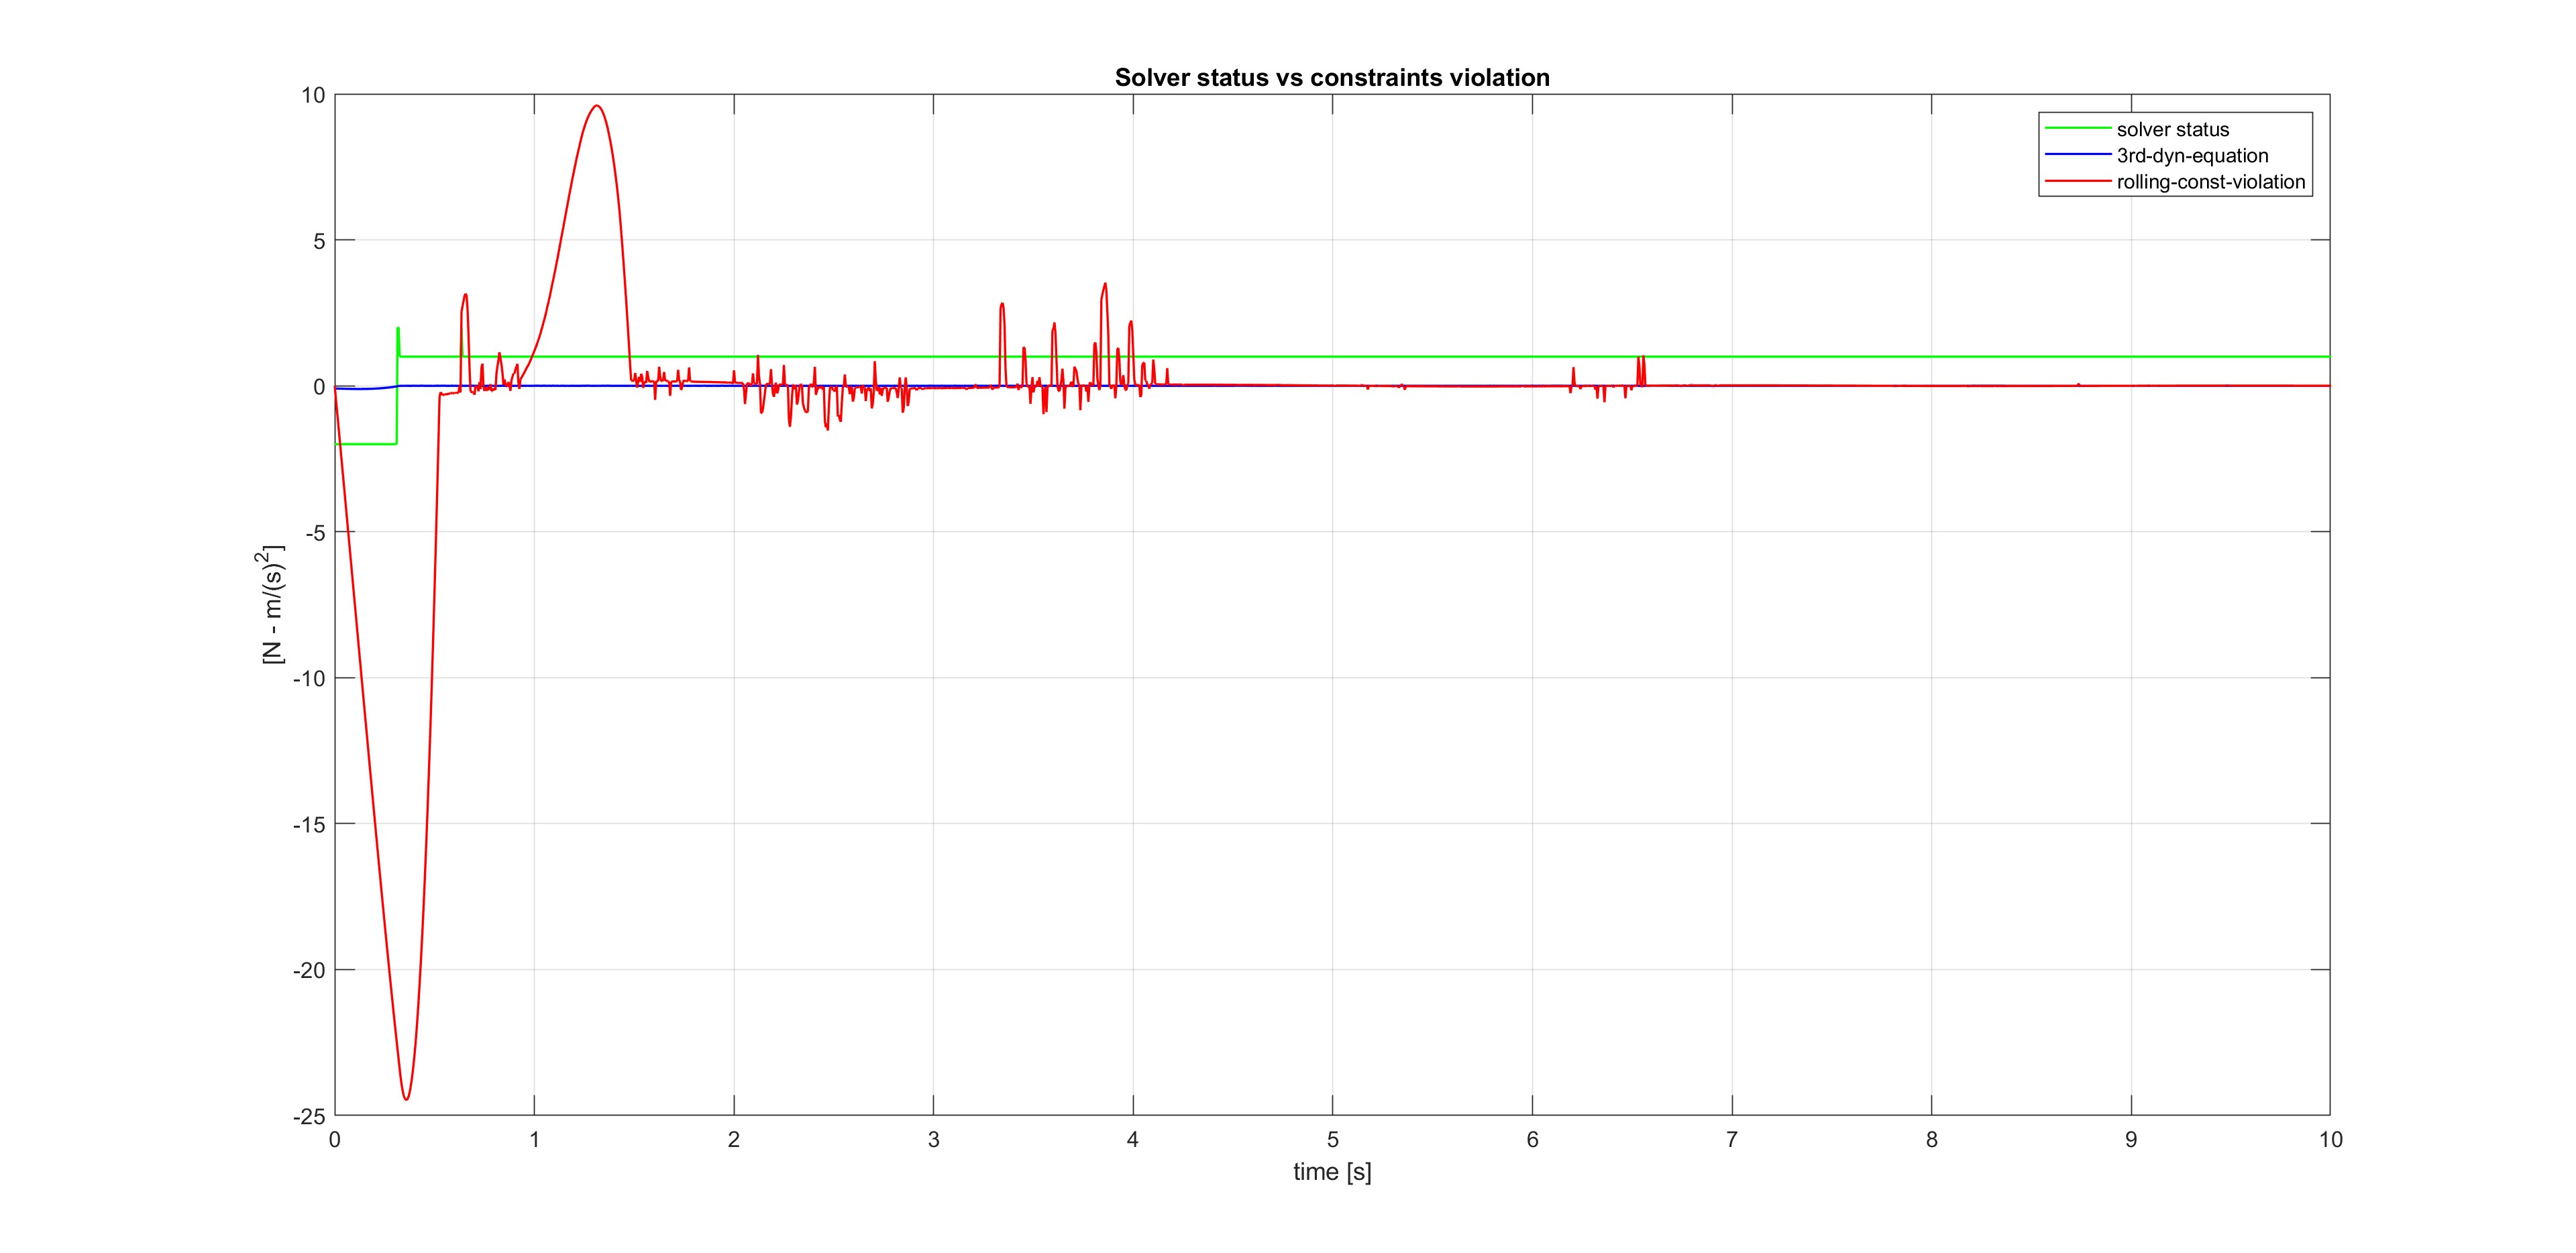
\includegraphics[width=1\linewidth]{Images/Robustness analysis/maximum load/Swing-Up/Slipping_velocity.jpg}
    \caption{Swing-up slipping velocity with disturbances in the case of maximum load.}
    \label{fig:Swing-up slipping velocity with disturbances in the case of maximum load}
\end{figure}

From Figure \ref{fig:Swing-up slipping velocity with disturbances in the case of maximum load}, representing in red the slipping velocity and in green the solver status, it can be noticed that for the first 0.5 seconds, the solver status is -2 due to an initial slipping velocity significantly different from zero. 

\section{Sinusoidal Trajectory with model uncertainties}
\label{sec:Sinusoidal Trajectory with model uncertainties}

Here we directly test a general nominal trajectory in the plane x-y for all the three conditions mentioned in the prologue of this chapter.

\subsection{Sinusoidal Trajectory in the unloaded case}
\label{subsec:Sinusoidal Trajectory in the unloaded case}

Figures \ref{fig:Sinusoidal trajectory position error with disturbances in the unloaded case} and \ref{fig:Sinusoidal trajectory velocity error with disturbances in the unloaded case}, show the nominal and actual trajectories in position and velocity respectively for the unloaded condition, and it can be noticed how, after the transient, the actual trajectories approach the nominal ones.
Some overshoots appear in Figure \ref{fig:Sinusoidal trajectory velocity error with disturbances in the unloaded case} due to the discontinuous acceleration profile.


\begin{figure}
    \centering
    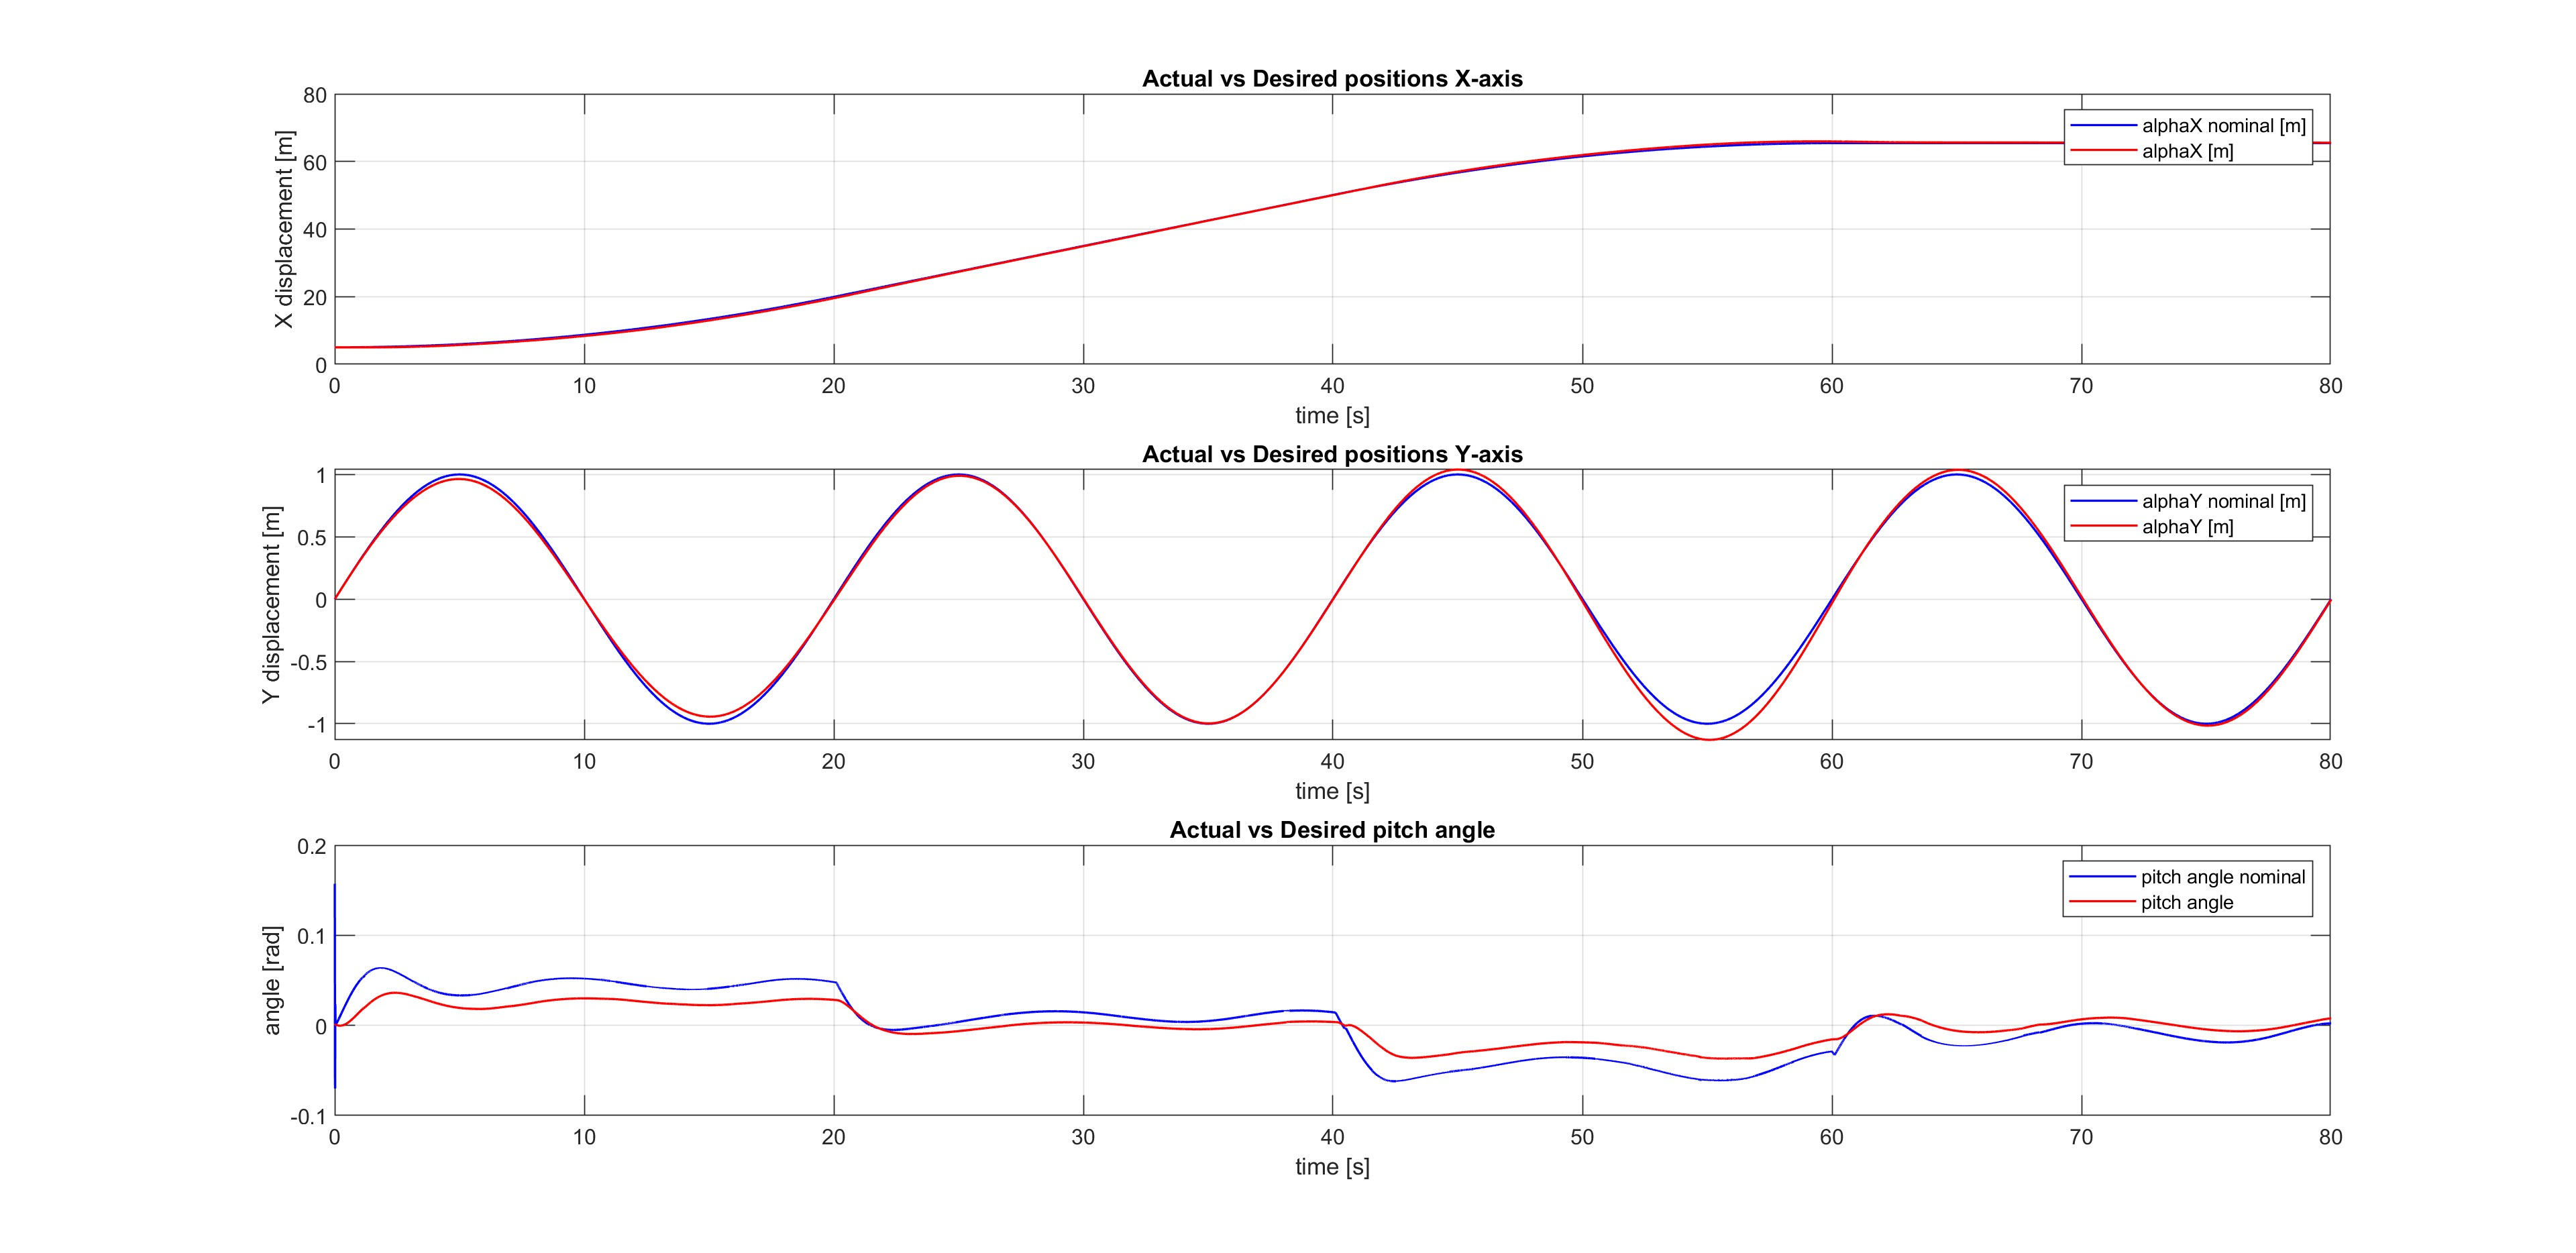
\includegraphics[width=1\linewidth]{Images/Robustness analysis/Unloaded/sinusoidal trajectory/Position_error.jpg}
    \caption{Sinusoidal trajectory position error with disturbances in the unloaded case.}
    \label{fig:Sinusoidal trajectory position error with disturbances in the unloaded case}
\end{figure}

\begin{figure}
    \centering
    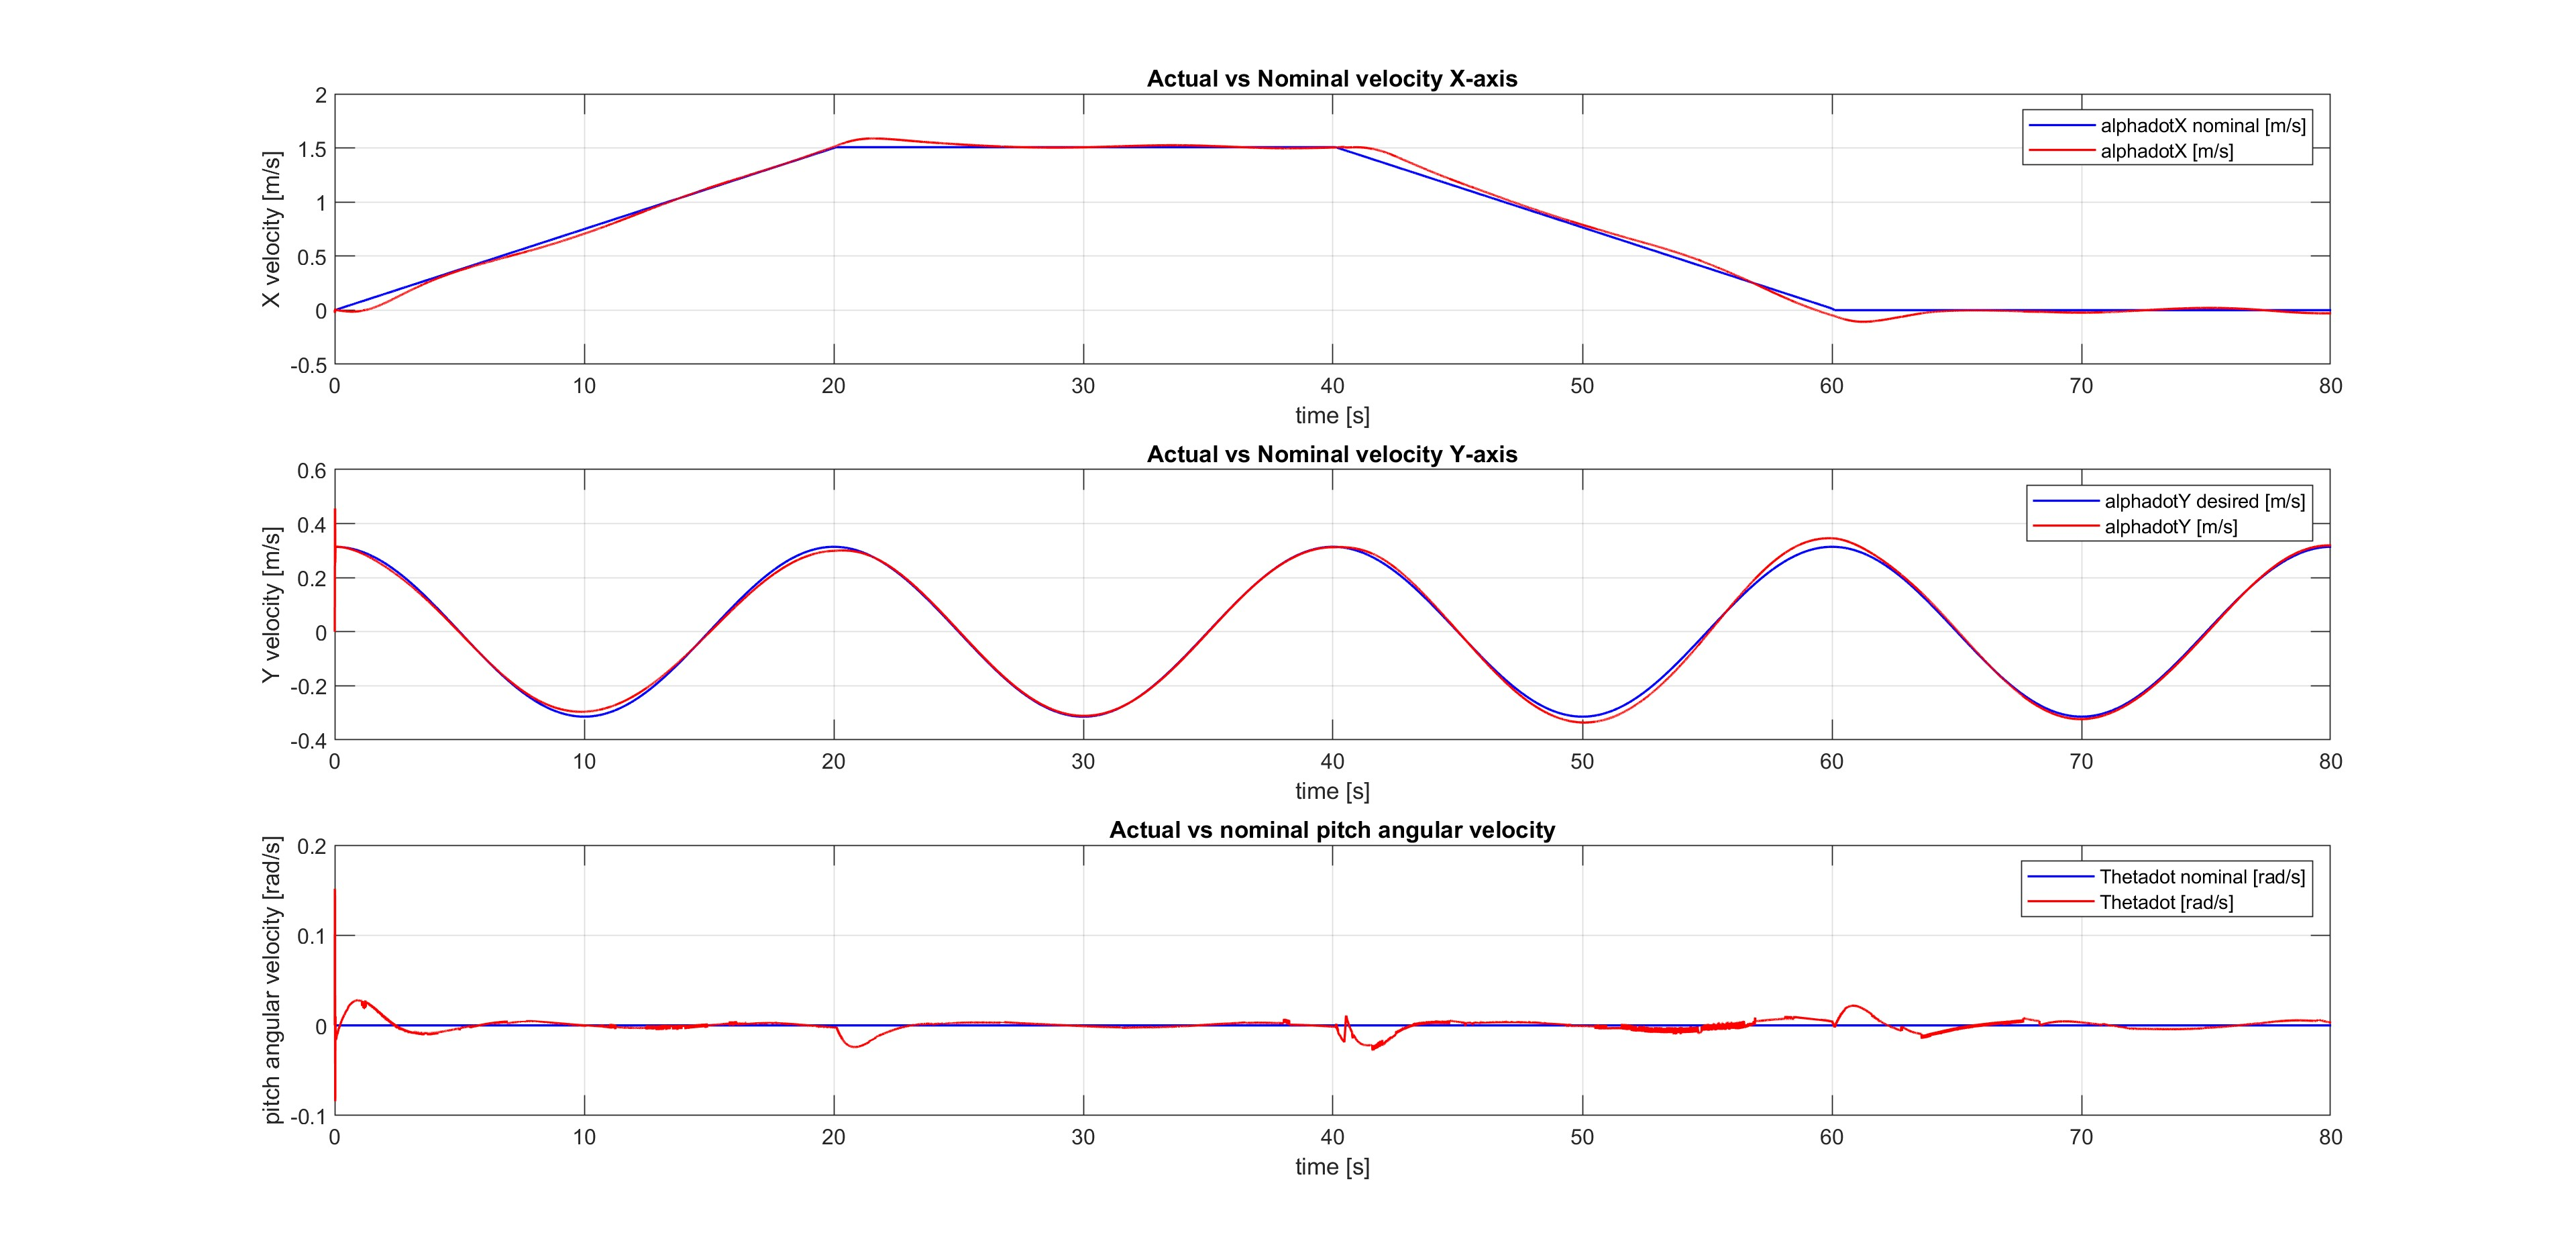
\includegraphics[width=1\linewidth]{Images/Robustness analysis/Unloaded/sinusoidal trajectory/Velocity_error.jpg}
    \caption{Sinusoidal trajectory velocity error with disturbances in the unloaded case.}
    \label{fig:Sinusoidal trajectory velocity error with disturbances in the unloaded case}
\end{figure}

Figure \ref{fig:Sinusoidal trajectory slipping velocity with disturbances in the unloaded case} instead shows in red the slipping velocity between the wheels and the terrain, and in green the solver status which is always =1.

\begin{figure}
    \centering
    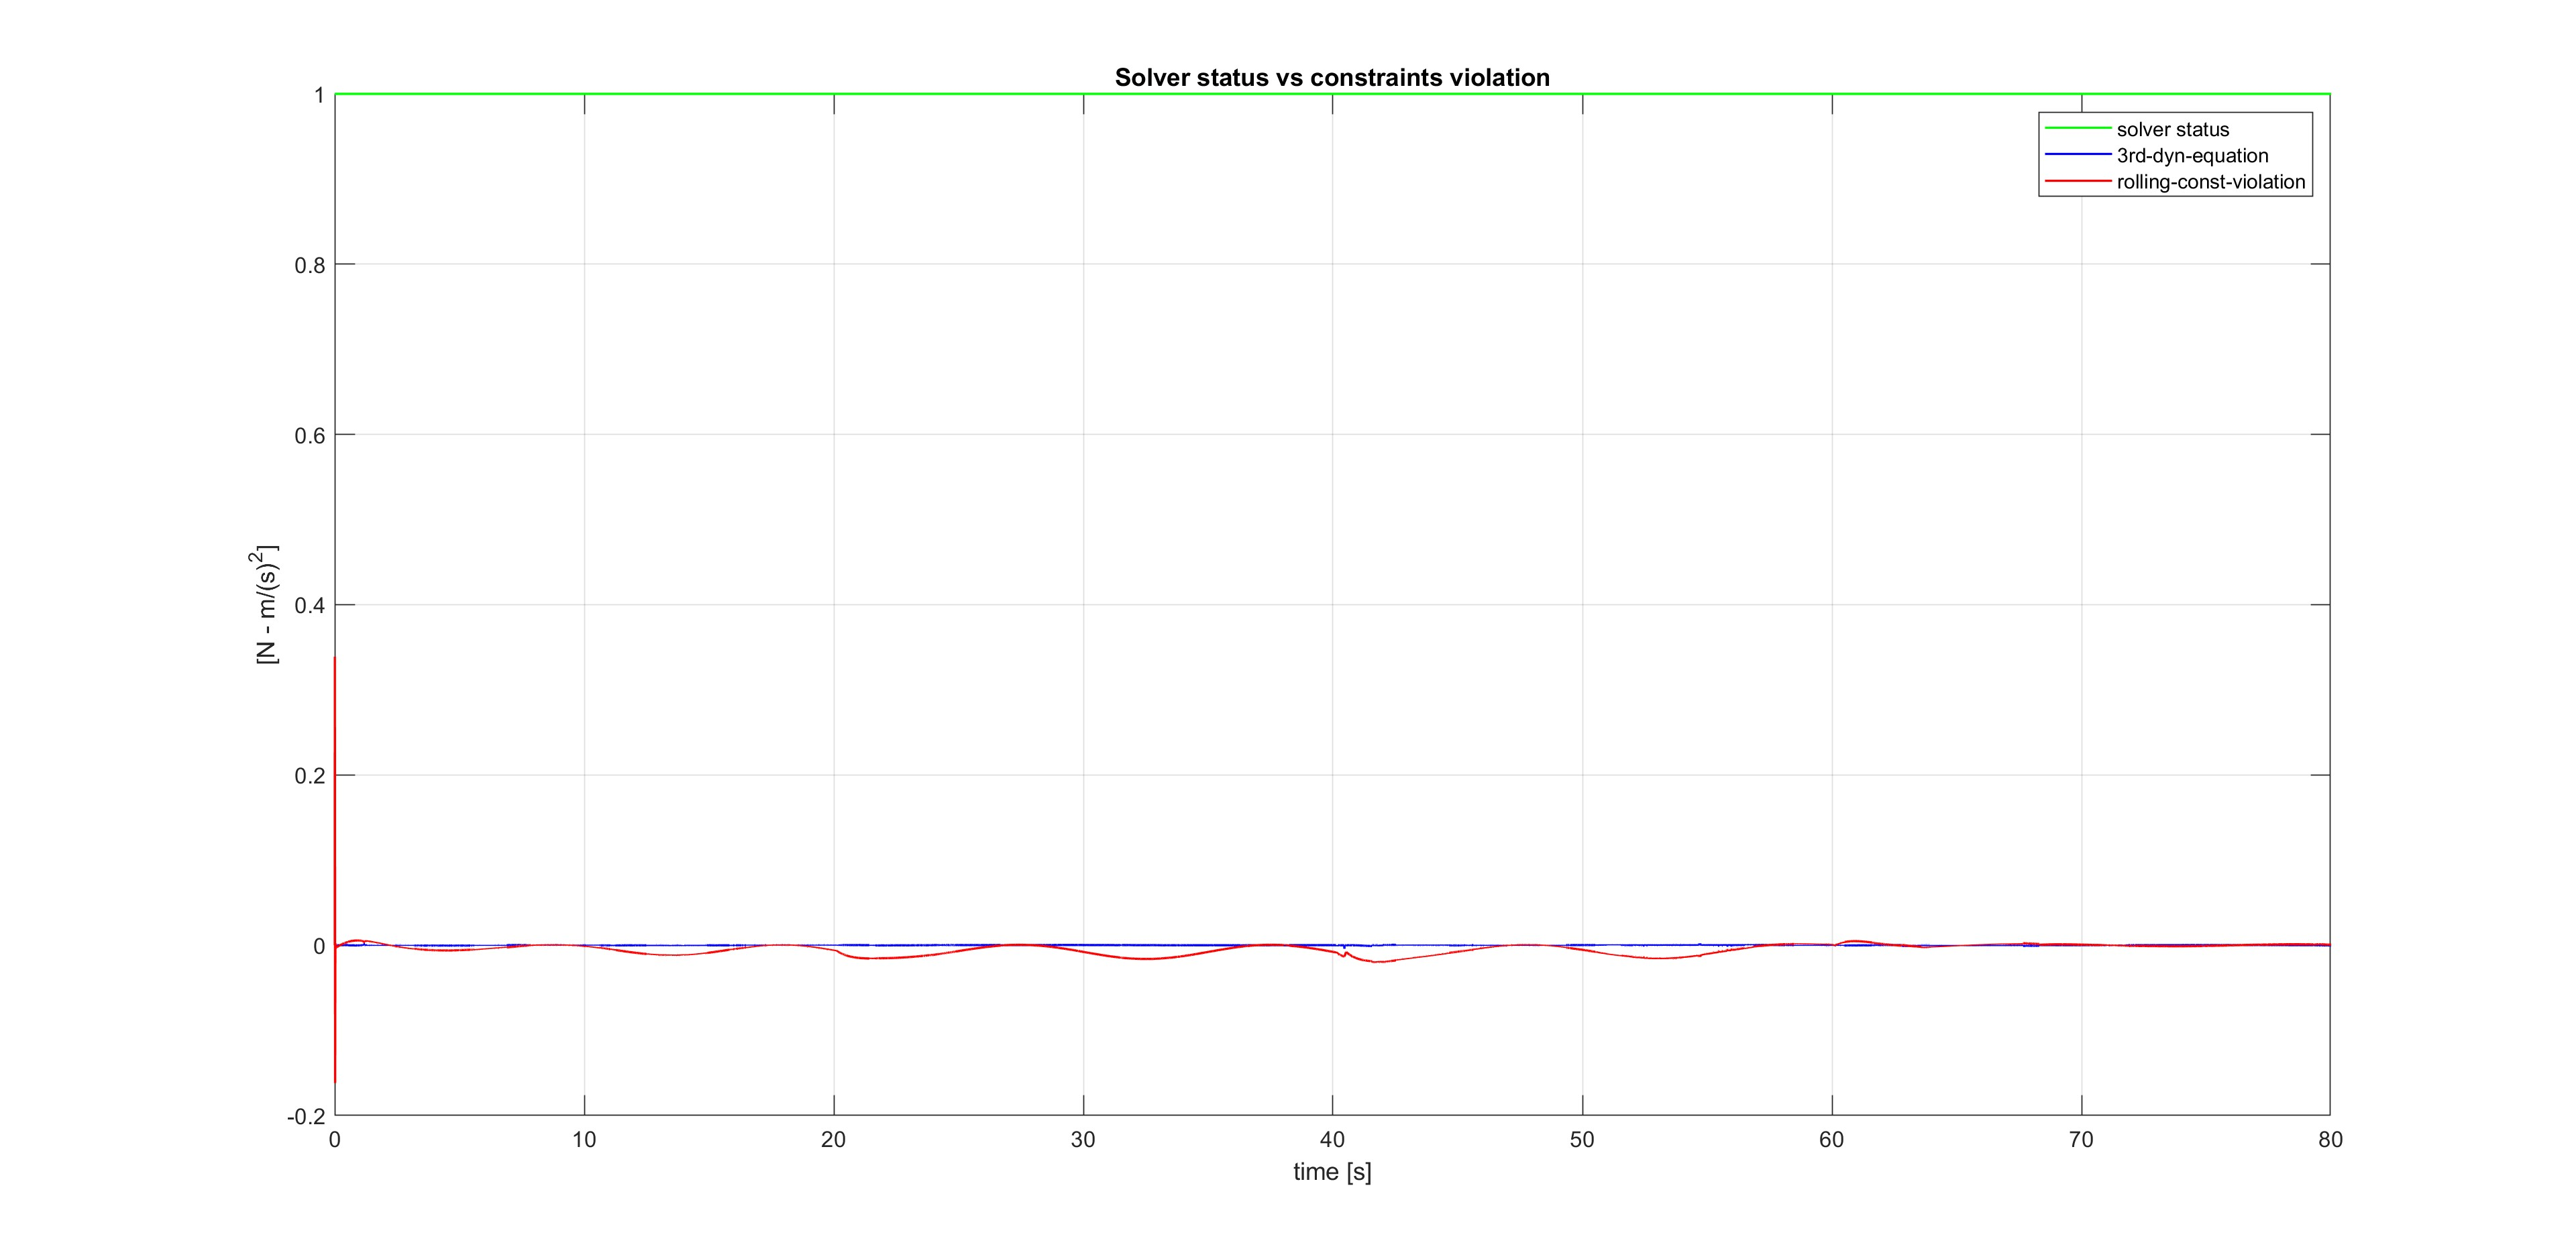
\includegraphics[width=1\linewidth]{Images/Robustness analysis/Unloaded/sinusoidal trajectory/Slipping_velocity.jpg}
    \caption{Sinusoidal trajectory slipping velocity with disturbances in the unloaded case.}
    \label{fig:Sinusoidal trajectory slipping velocity with disturbances in the unloaded case}
\end{figure}


\subsection{Sinusoidal Trajectory in the case of half load}
\label{subsec:Sinusoidal Trajectory in the case of half load}

Figures \ref{fig:Sinusoidal trajectory position error with disturbances in the case of half load} and \ref{fig:Sinusoidal trajectory velocity error with disturbances in the case of half load}, show the nominal and actual trajectories in position and velocity respectively for the condition of half load, and also in this case, after the transient, the actual trajectories approach the nominal ones.
Also in this case, some overshoots appear in Figure \ref{fig:Sinusoidal trajectory velocity error with disturbances in the case of half load} due to the discontinuous acceleration profile.

\begin{figure}
    \centering
    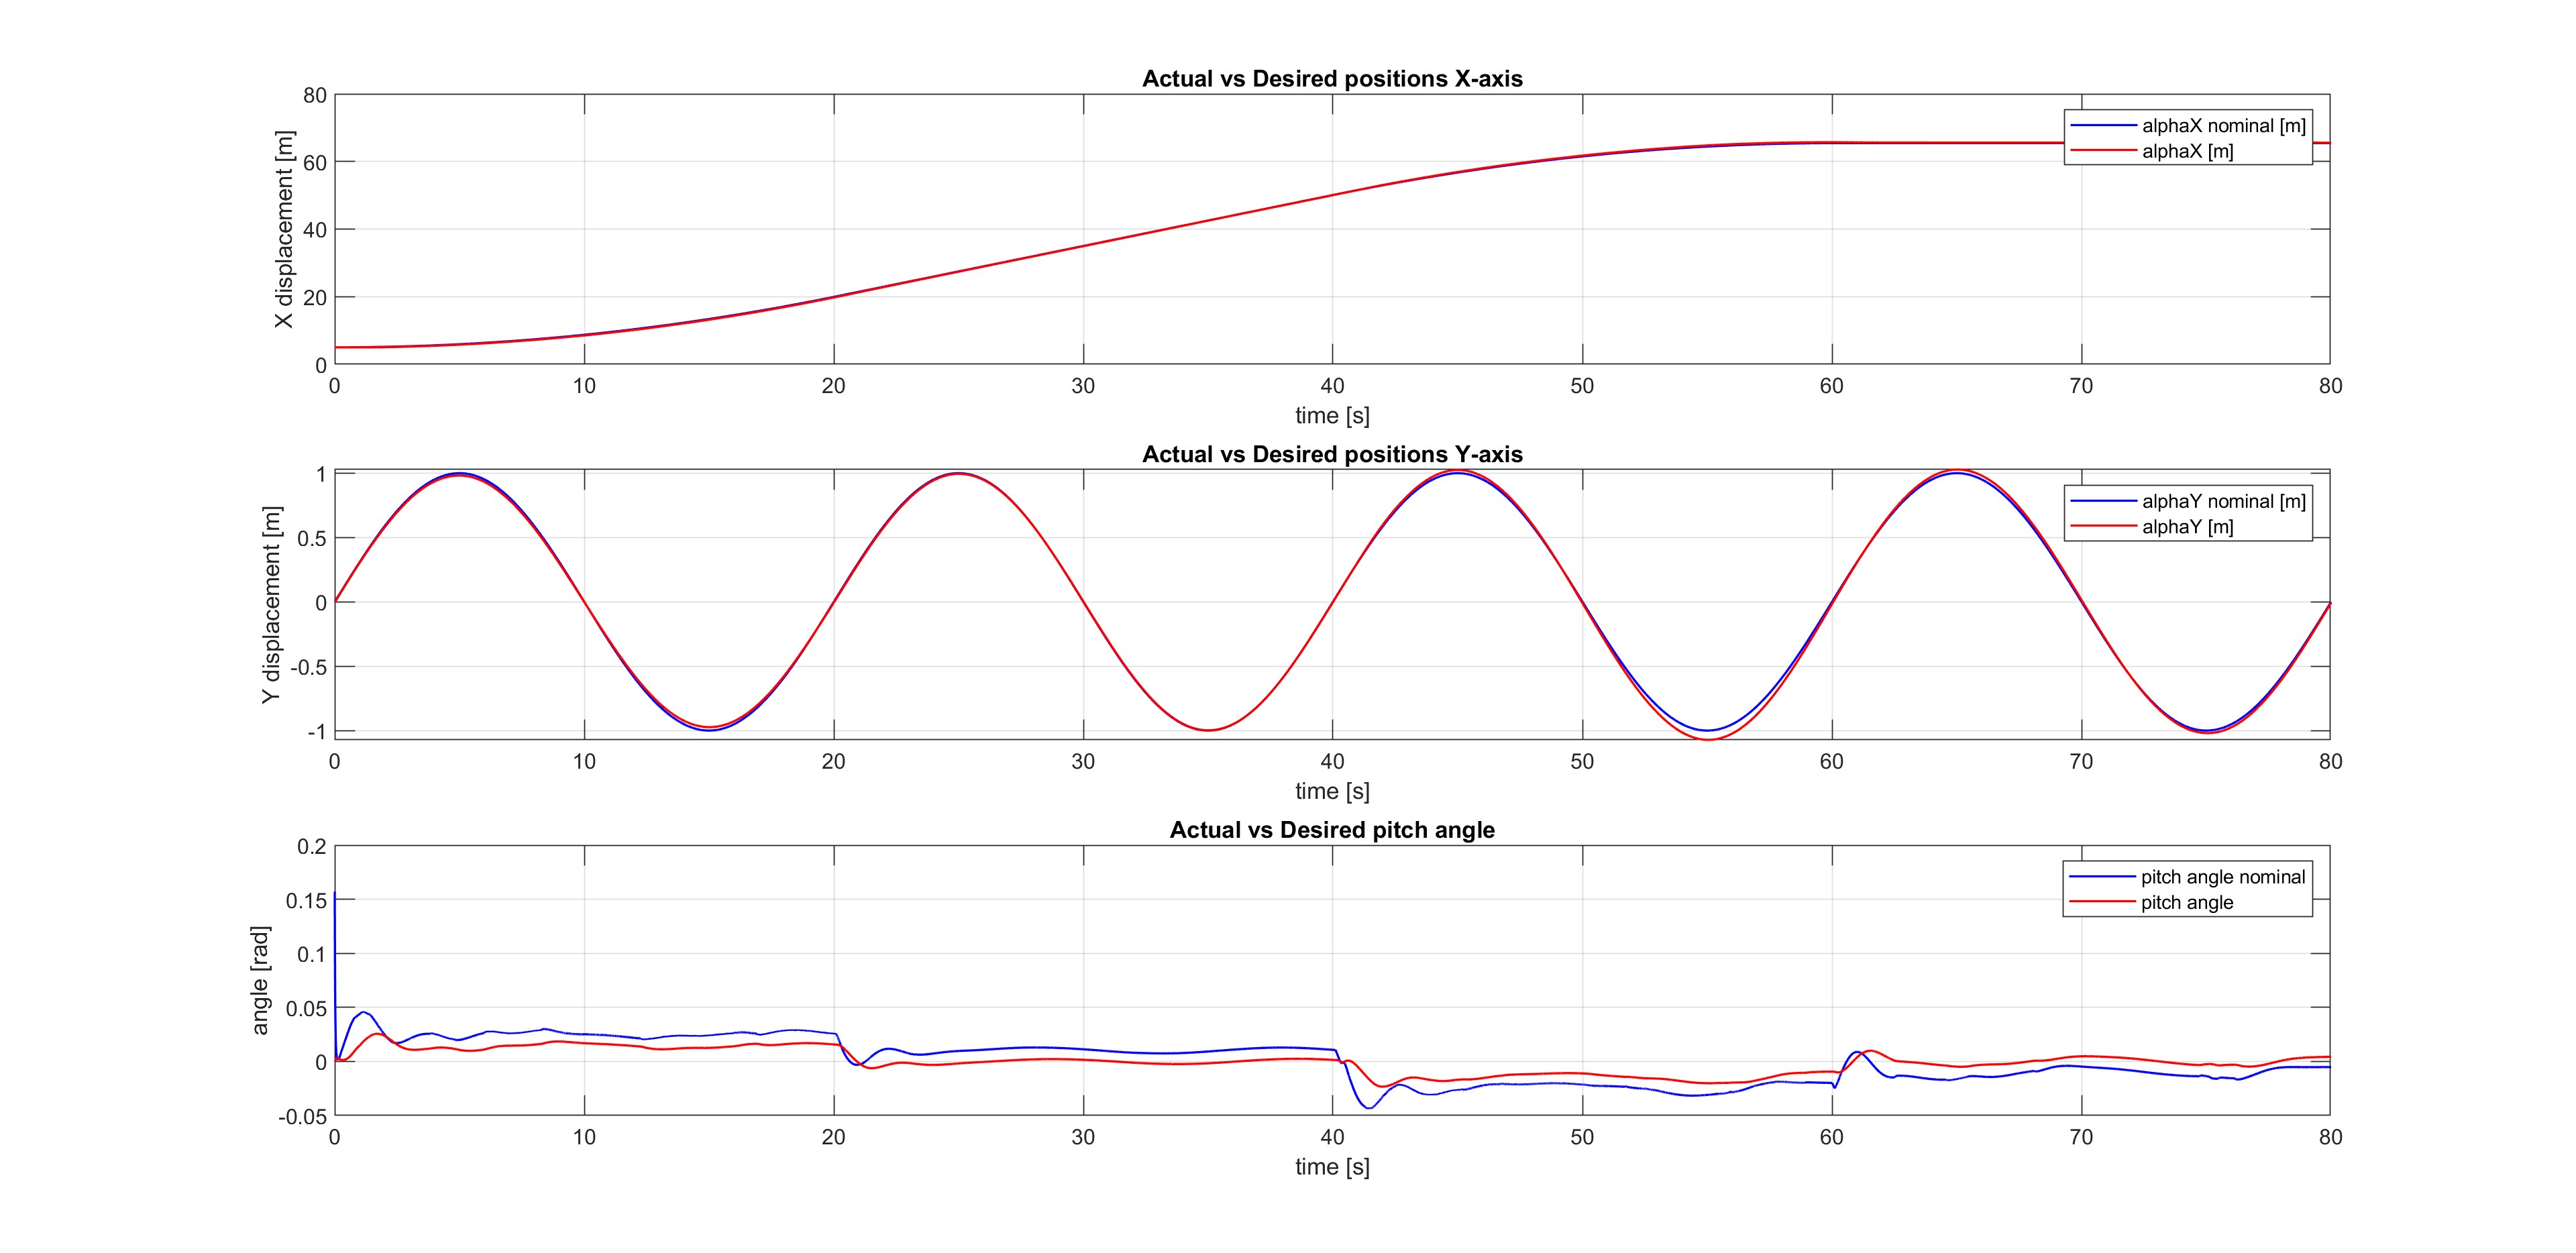
\includegraphics[width=1\linewidth]{Images/Robustness analysis/intermediate load/sinusoidal trajectory/Position_error.jpg}
    \caption{Sinusoidal trajectory position error with disturbances in the case of half load.}
    \label{fig:Sinusoidal trajectory position error with disturbances in the case of half load}
\end{figure}

\begin{figure}
    \centering
    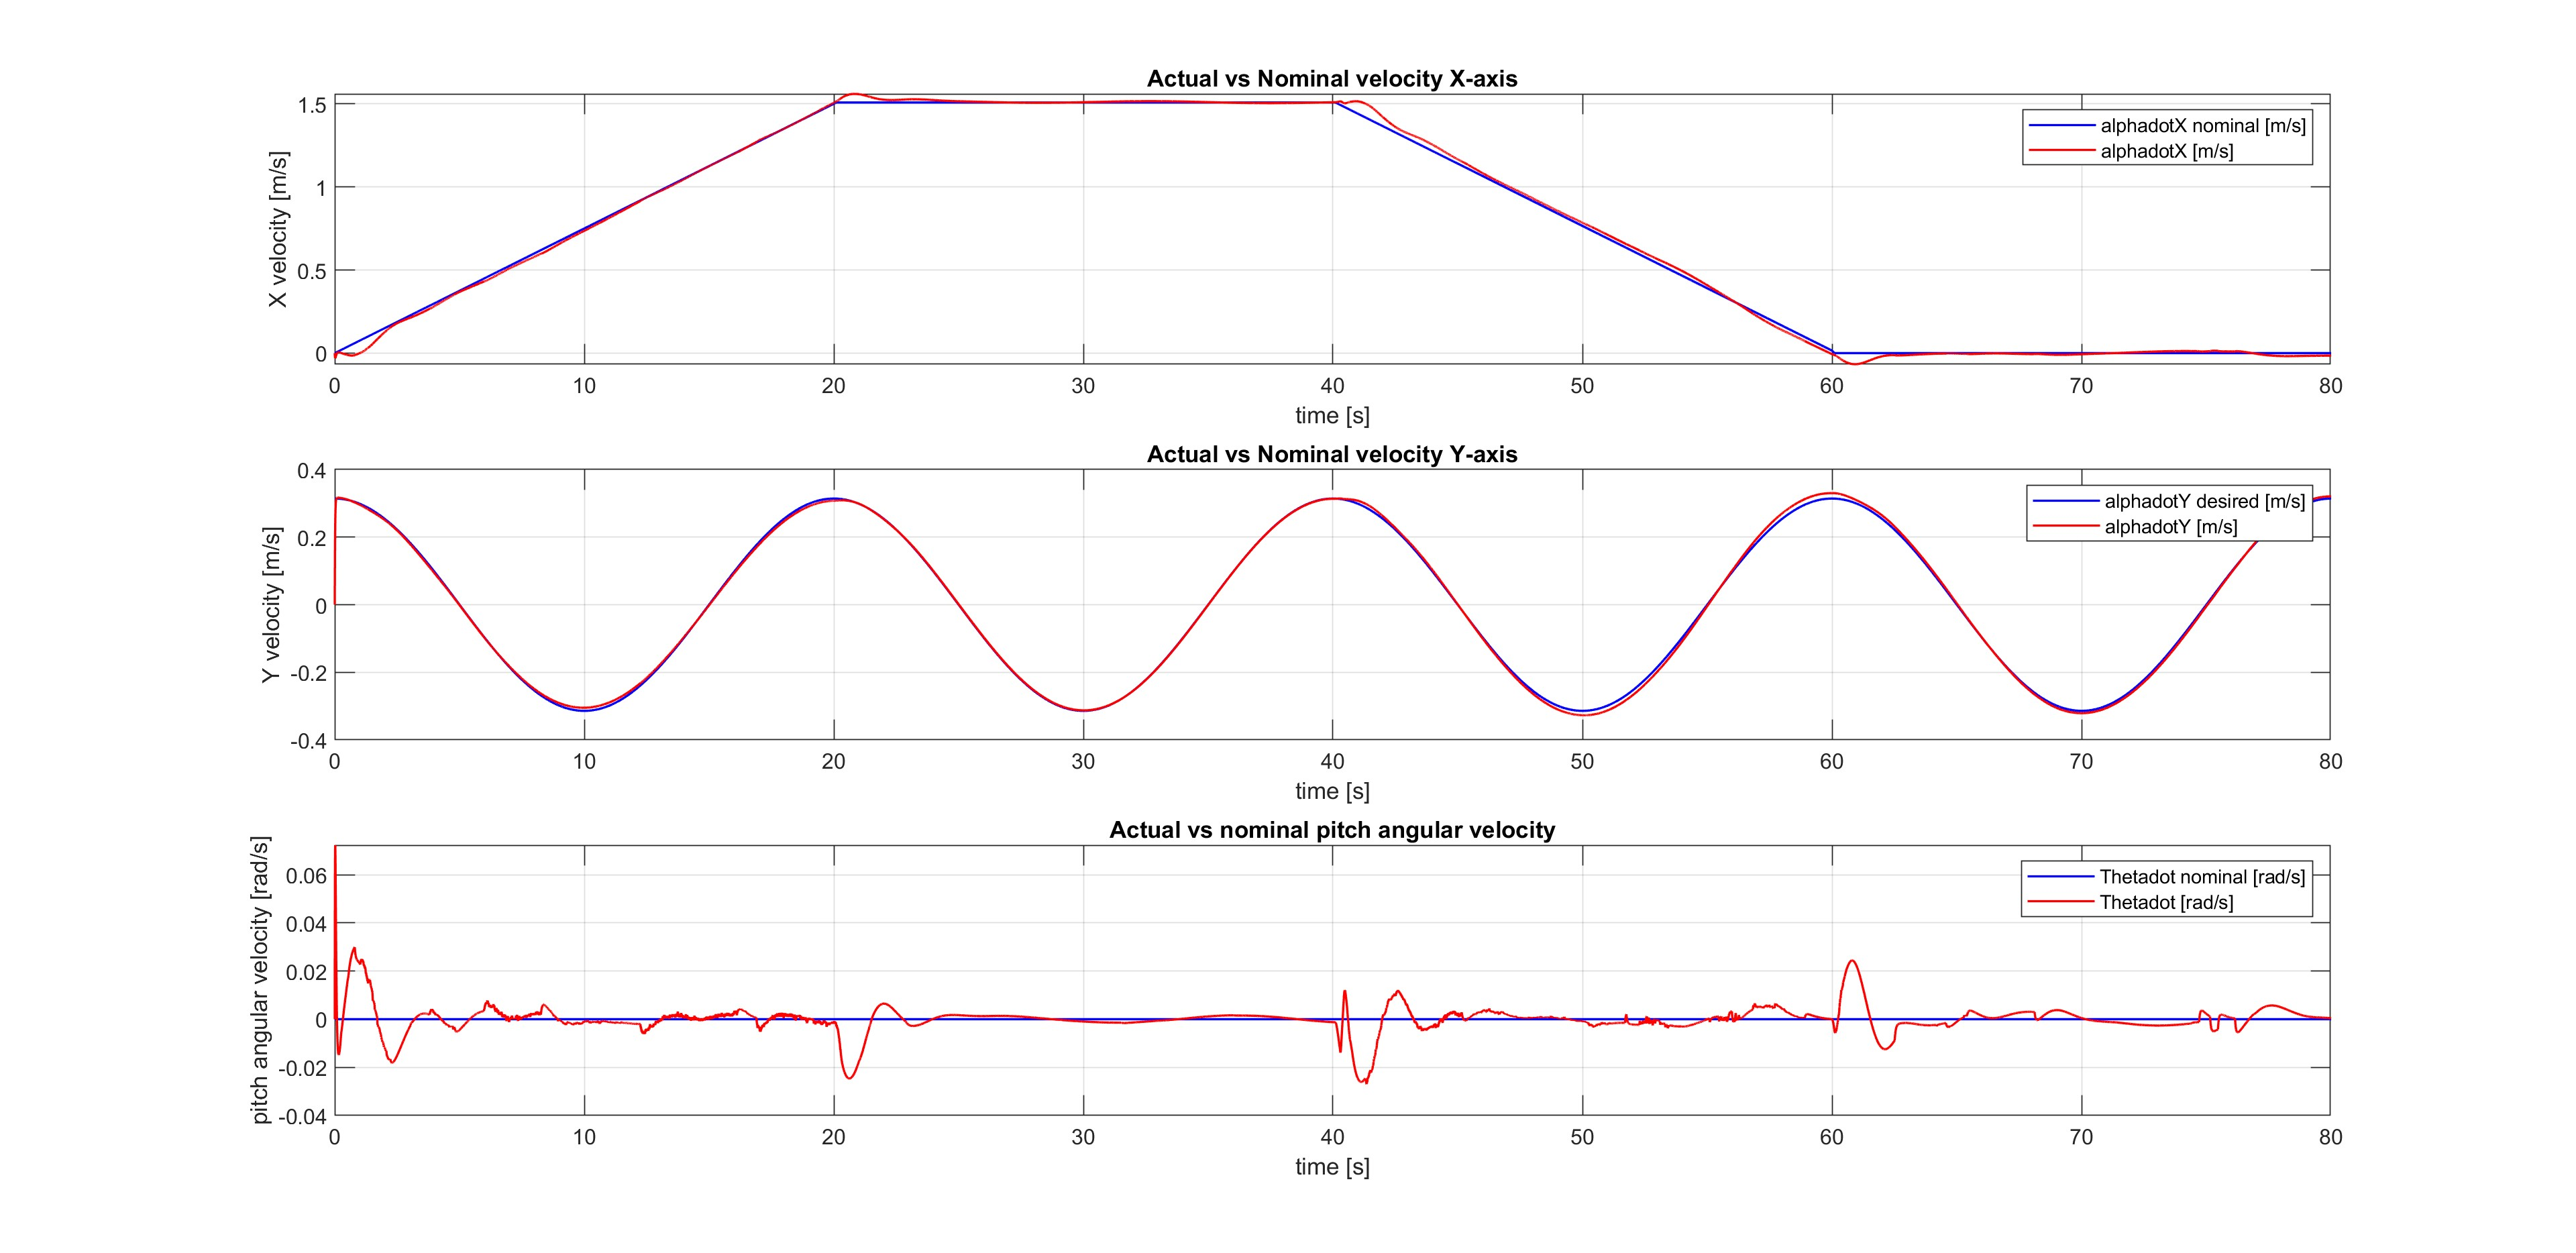
\includegraphics[width=1\linewidth]{Images/Robustness analysis/intermediate load/sinusoidal trajectory/Velocity_error.jpg}
    \caption{Sinusoidal trajectory velocity error with disturbances in the case of half load.}
    \label{fig:Sinusoidal trajectory velocity error with disturbances in the case of half load}
\end{figure}

Figure \ref{fig:Sinusoidal trajectory slipping velocity with disturbances in the case of half load} instead shows in red the slipping velocity between the wheels and the terrain which is almost zero, and in green the solver status which is always =1.

\begin{figure}
    \centering
    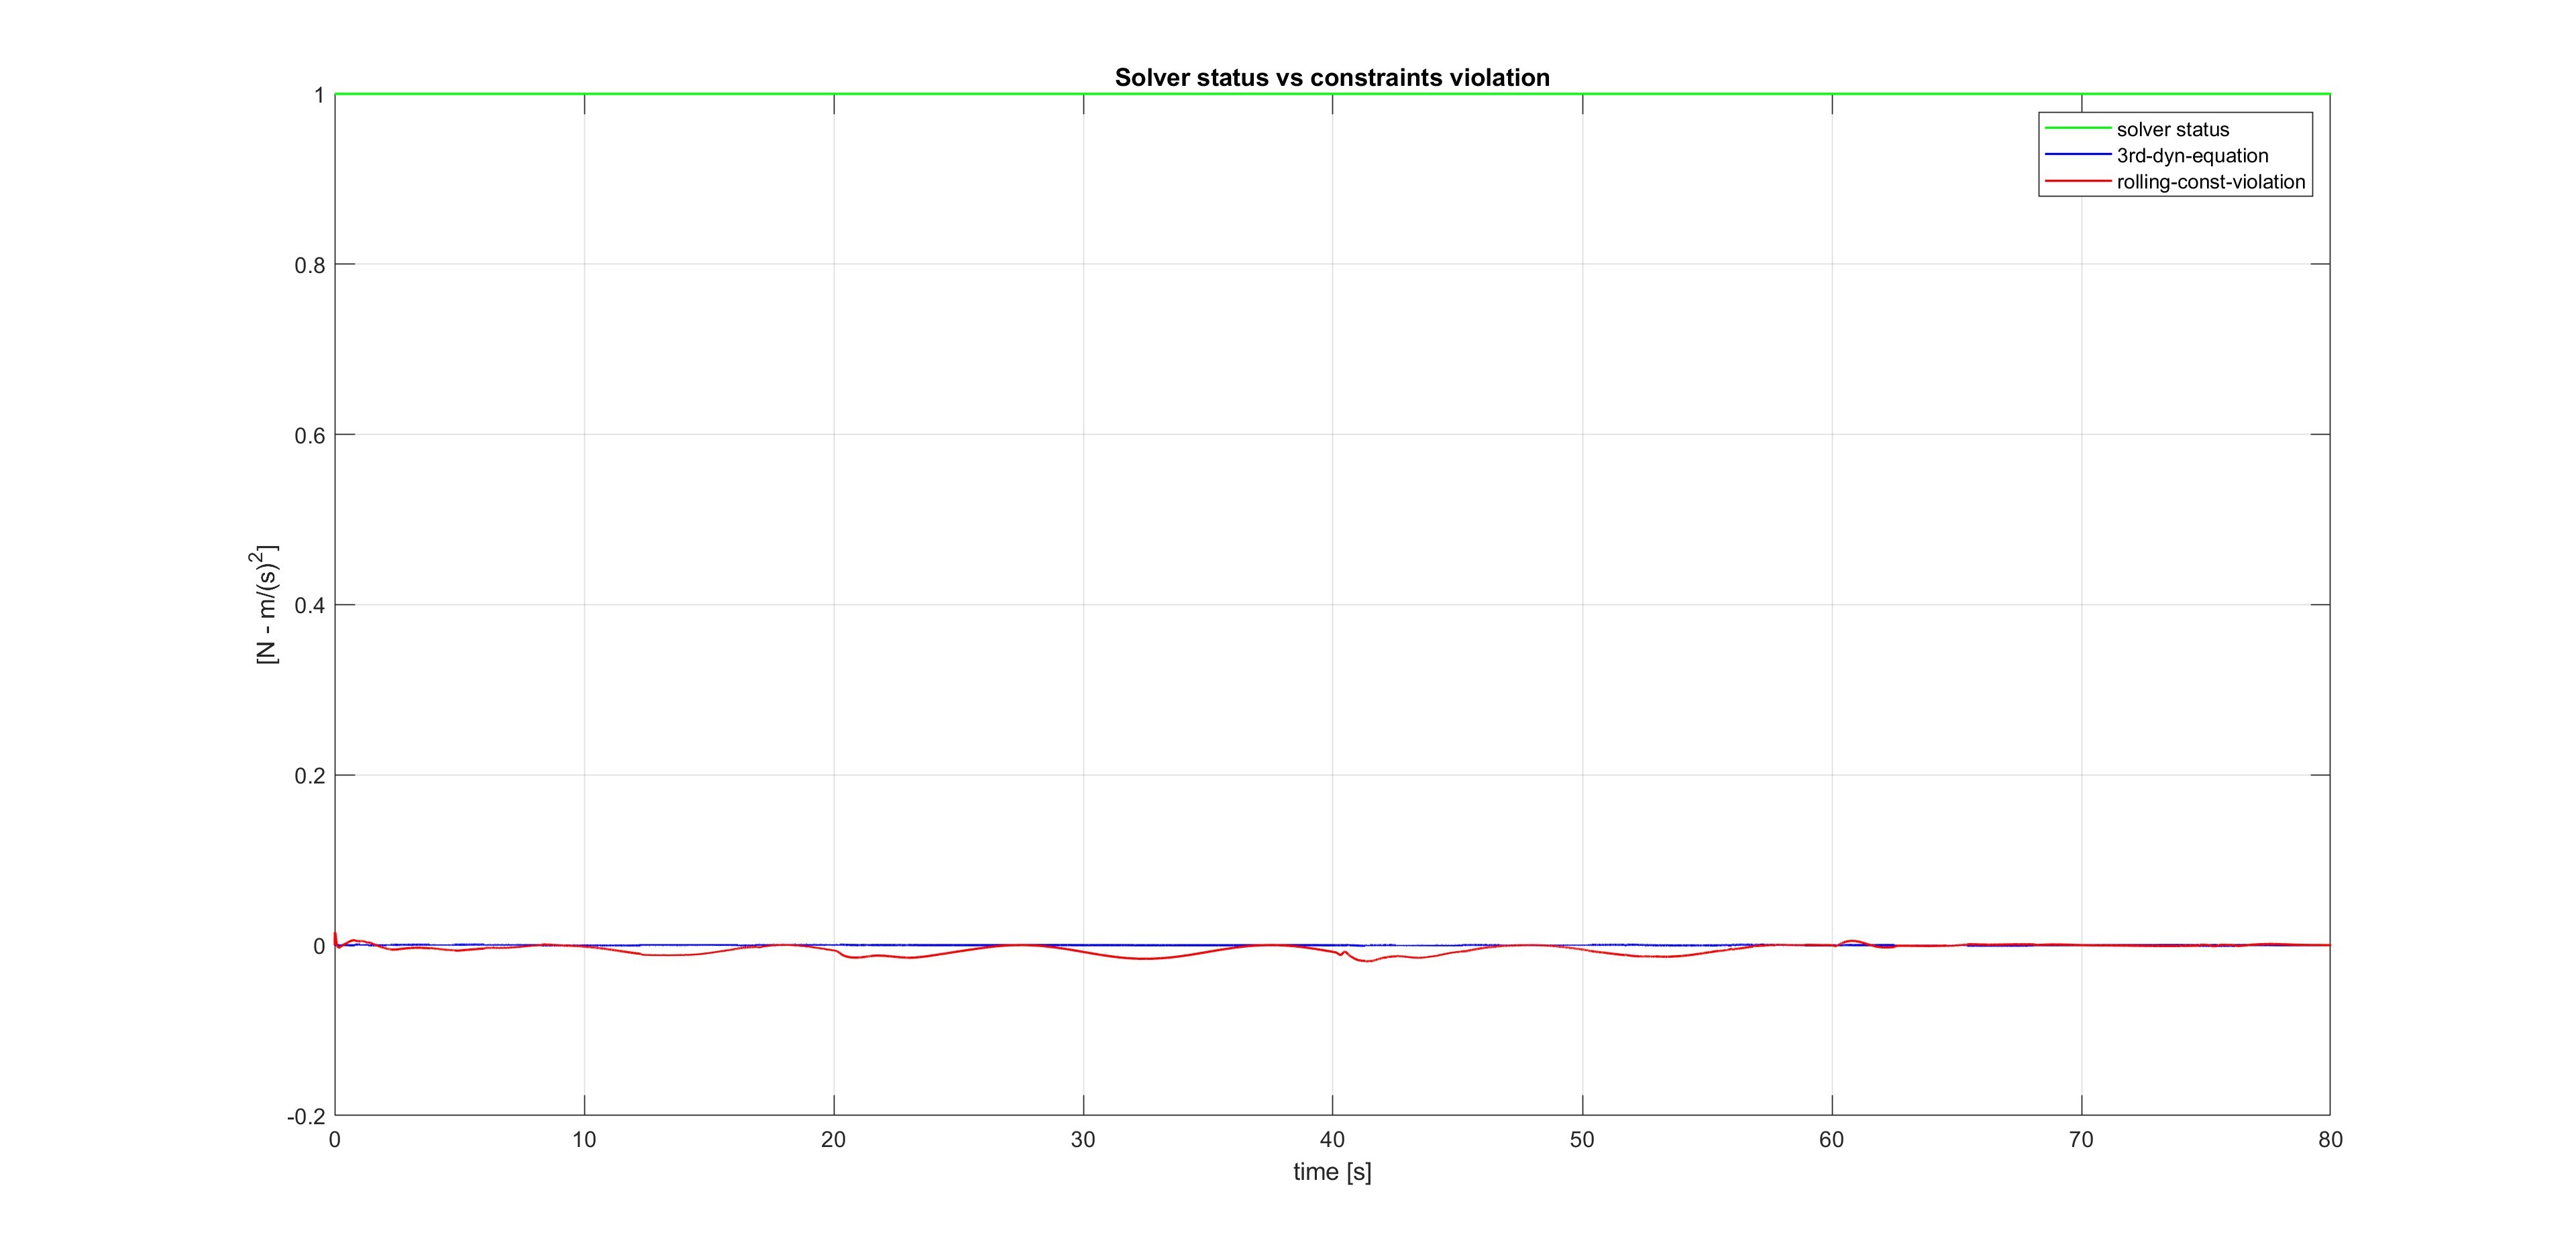
\includegraphics[width=1\linewidth]{Images/Robustness analysis/intermediate load/sinusoidal trajectory/Slipping_velocity.jpg}
    \caption{Sinusoidal trajectory slipping velocity with disturbances in the case of half load.}
    \label{fig:Sinusoidal trajectory slipping velocity with disturbances in the case of half load}
\end{figure}

\subsection{Sinusoidal Trajectory in the case of maximum load}
\label{subsec:Sinusoidal Trajectory in the case of maximum load}

Figures \ref{fig:Sinusoidal trajectory position error with disturbances in the case of maximum load} and \ref{fig:Sinusoidal trajectory velocity error with disturbances in the case of maximum load}, show the nominal and actual trajectories in position and velocity respectively for the worse case scenario in which the E-Cargo is loaded at its maximum capacity.
Also in this last case some overshoots can be noticed in Figure \ref{fig:Sinusoidal trajectory velocity error with disturbances in the unloaded case} due to the discontinuous acceleration profile.

\begin{figure}
    \centering
    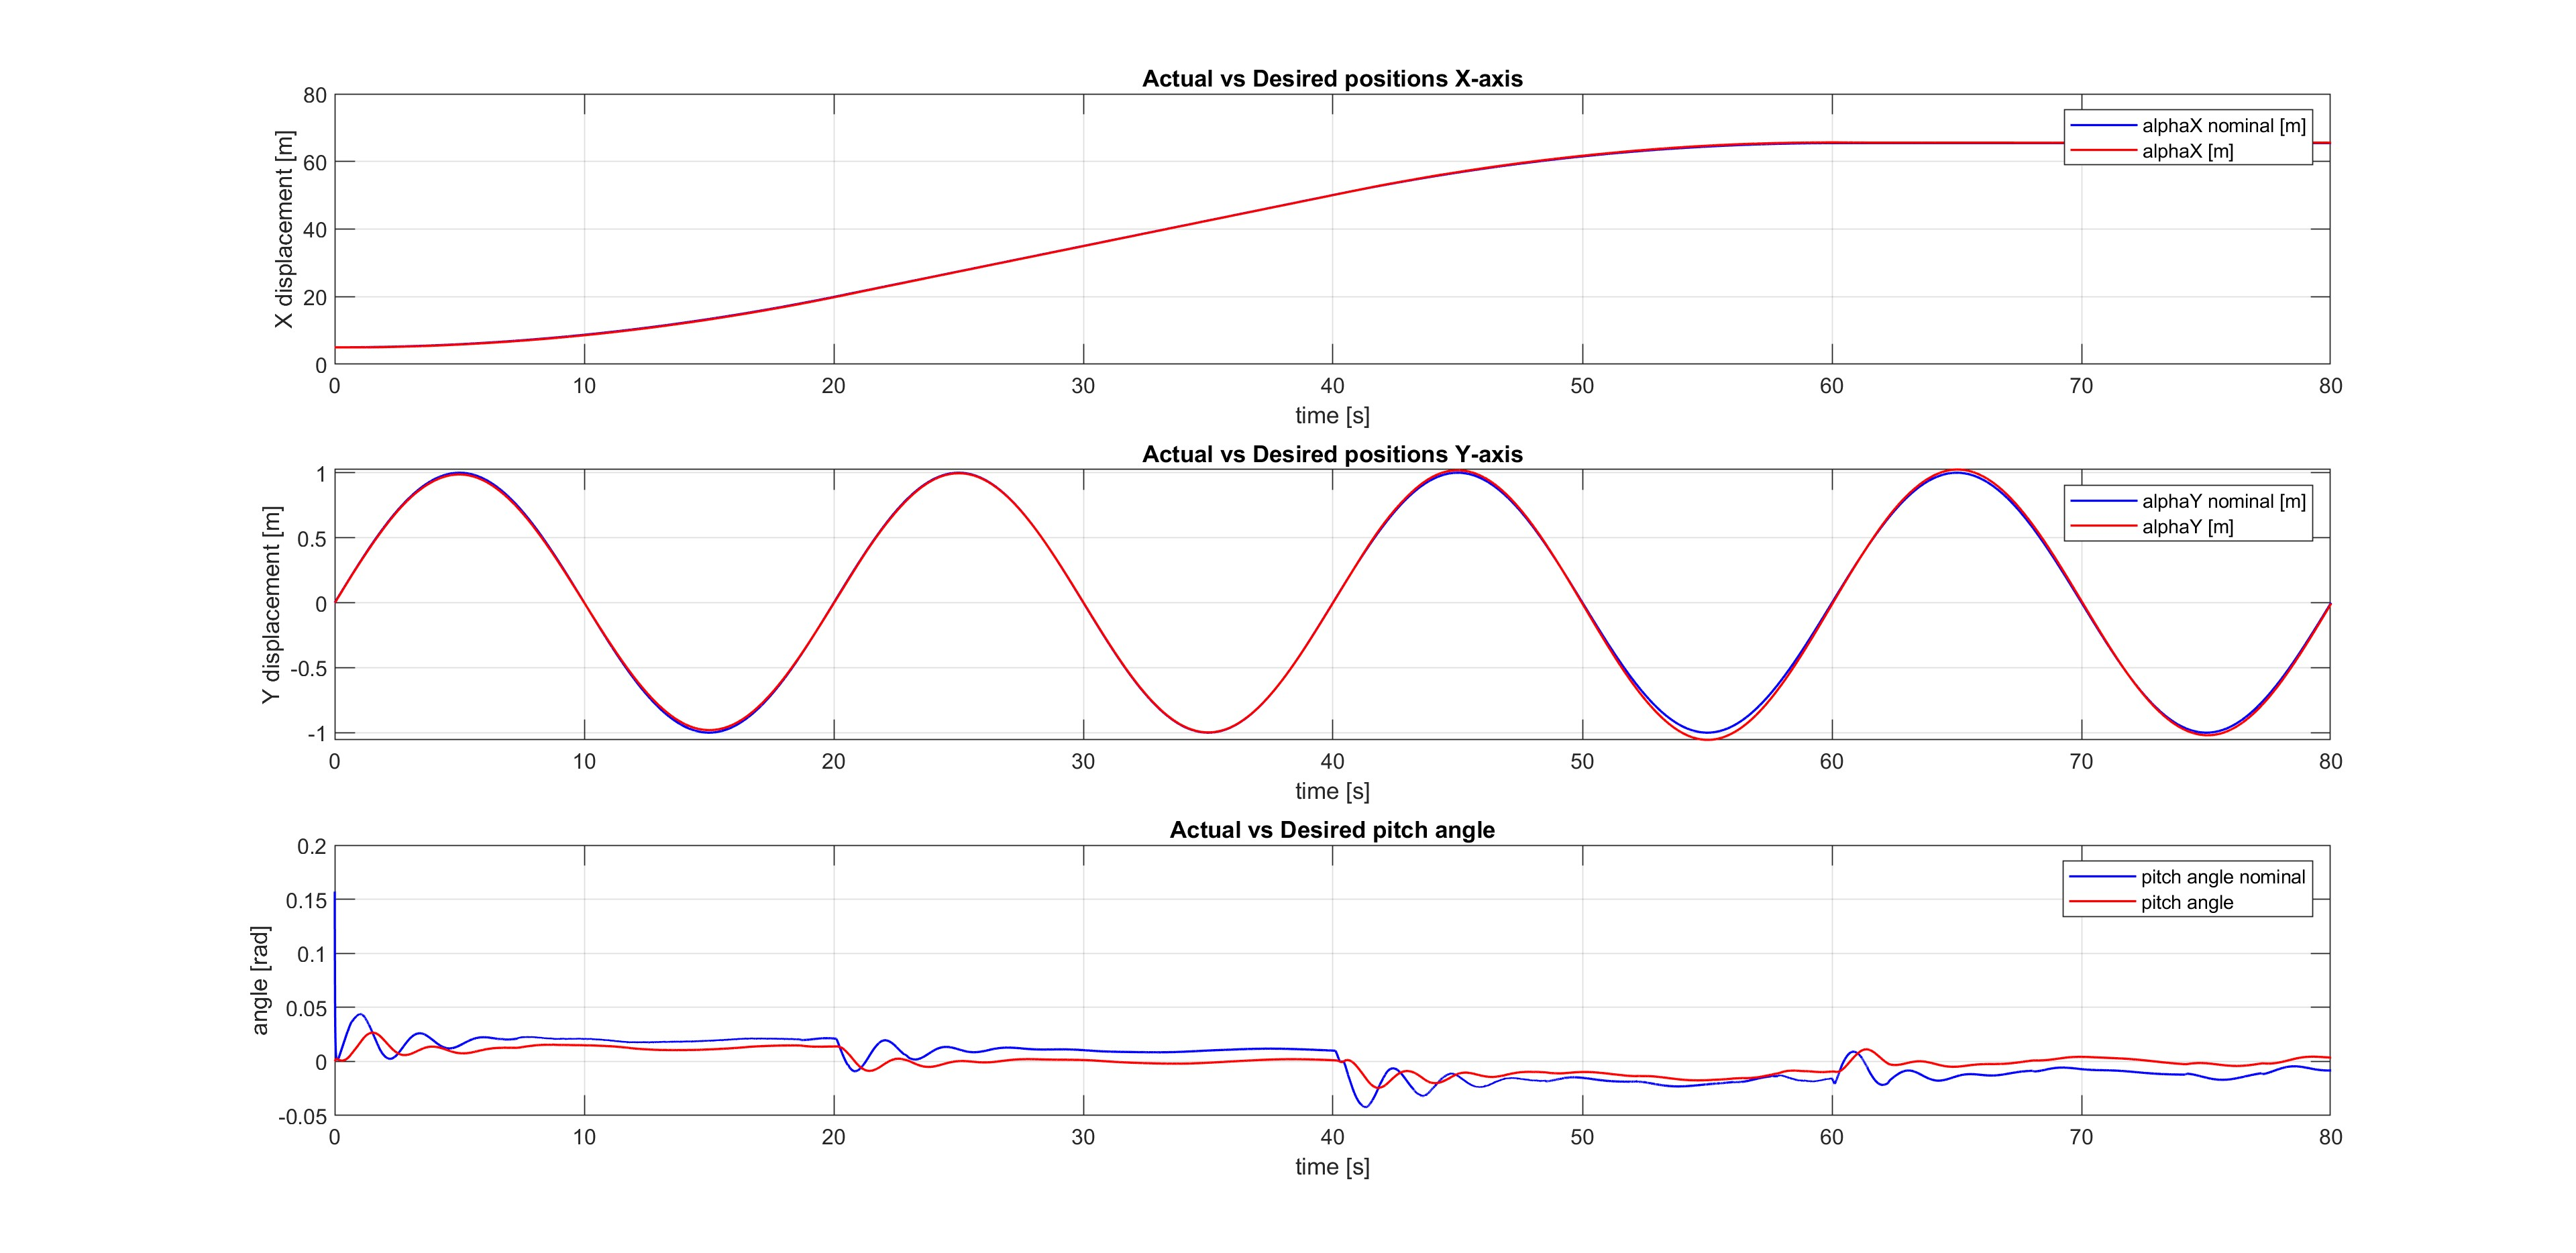
\includegraphics[width=1\linewidth]{Images/Robustness analysis/maximum load/sinusoidal trajectory/Position_error.jpg}
    \caption{Sinusoidal trajectory position error with disturbances in the case of maximum load.}
    \label{fig:Sinusoidal trajectory position error with disturbances in the case of maximum load}
\end{figure}

\begin{figure}
    \centering
    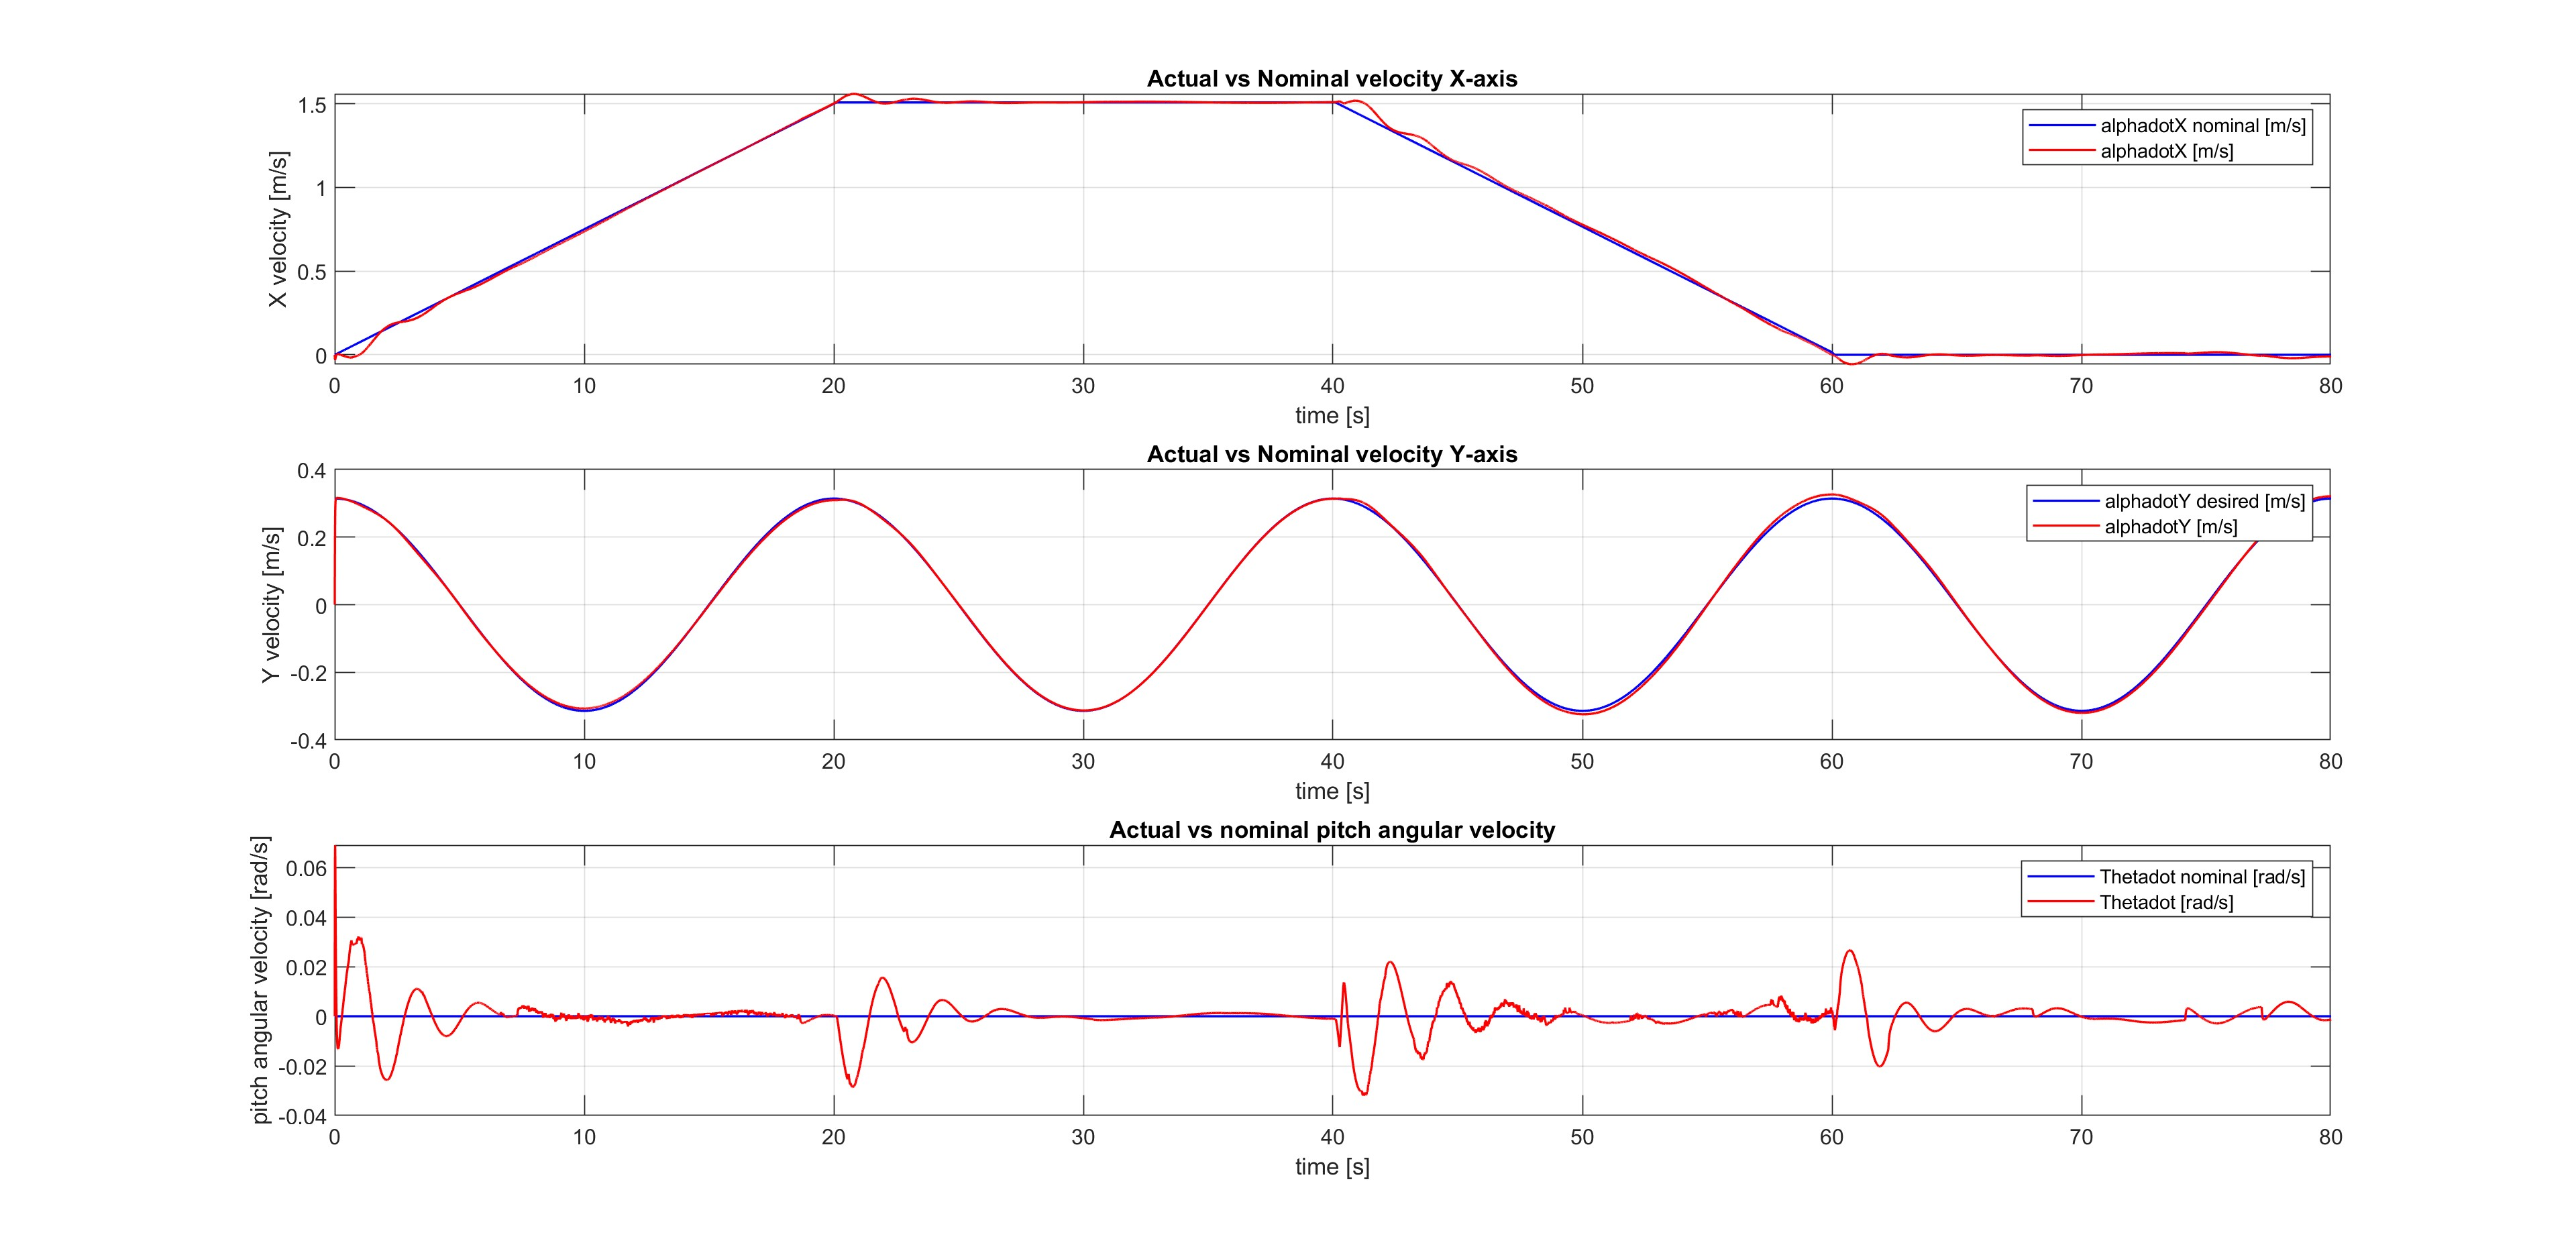
\includegraphics[width=1\linewidth]{Images/Robustness analysis/maximum load/sinusoidal trajectory/Velocity_error.jpg}
    \caption{Sinusoidal trajectory velocity error with disturbances in the case of maximum load.}
    \label{fig:Sinusoidal trajectory velocity error with disturbances in the case of maximum load}
\end{figure}

\begin{figure}
    \centering
    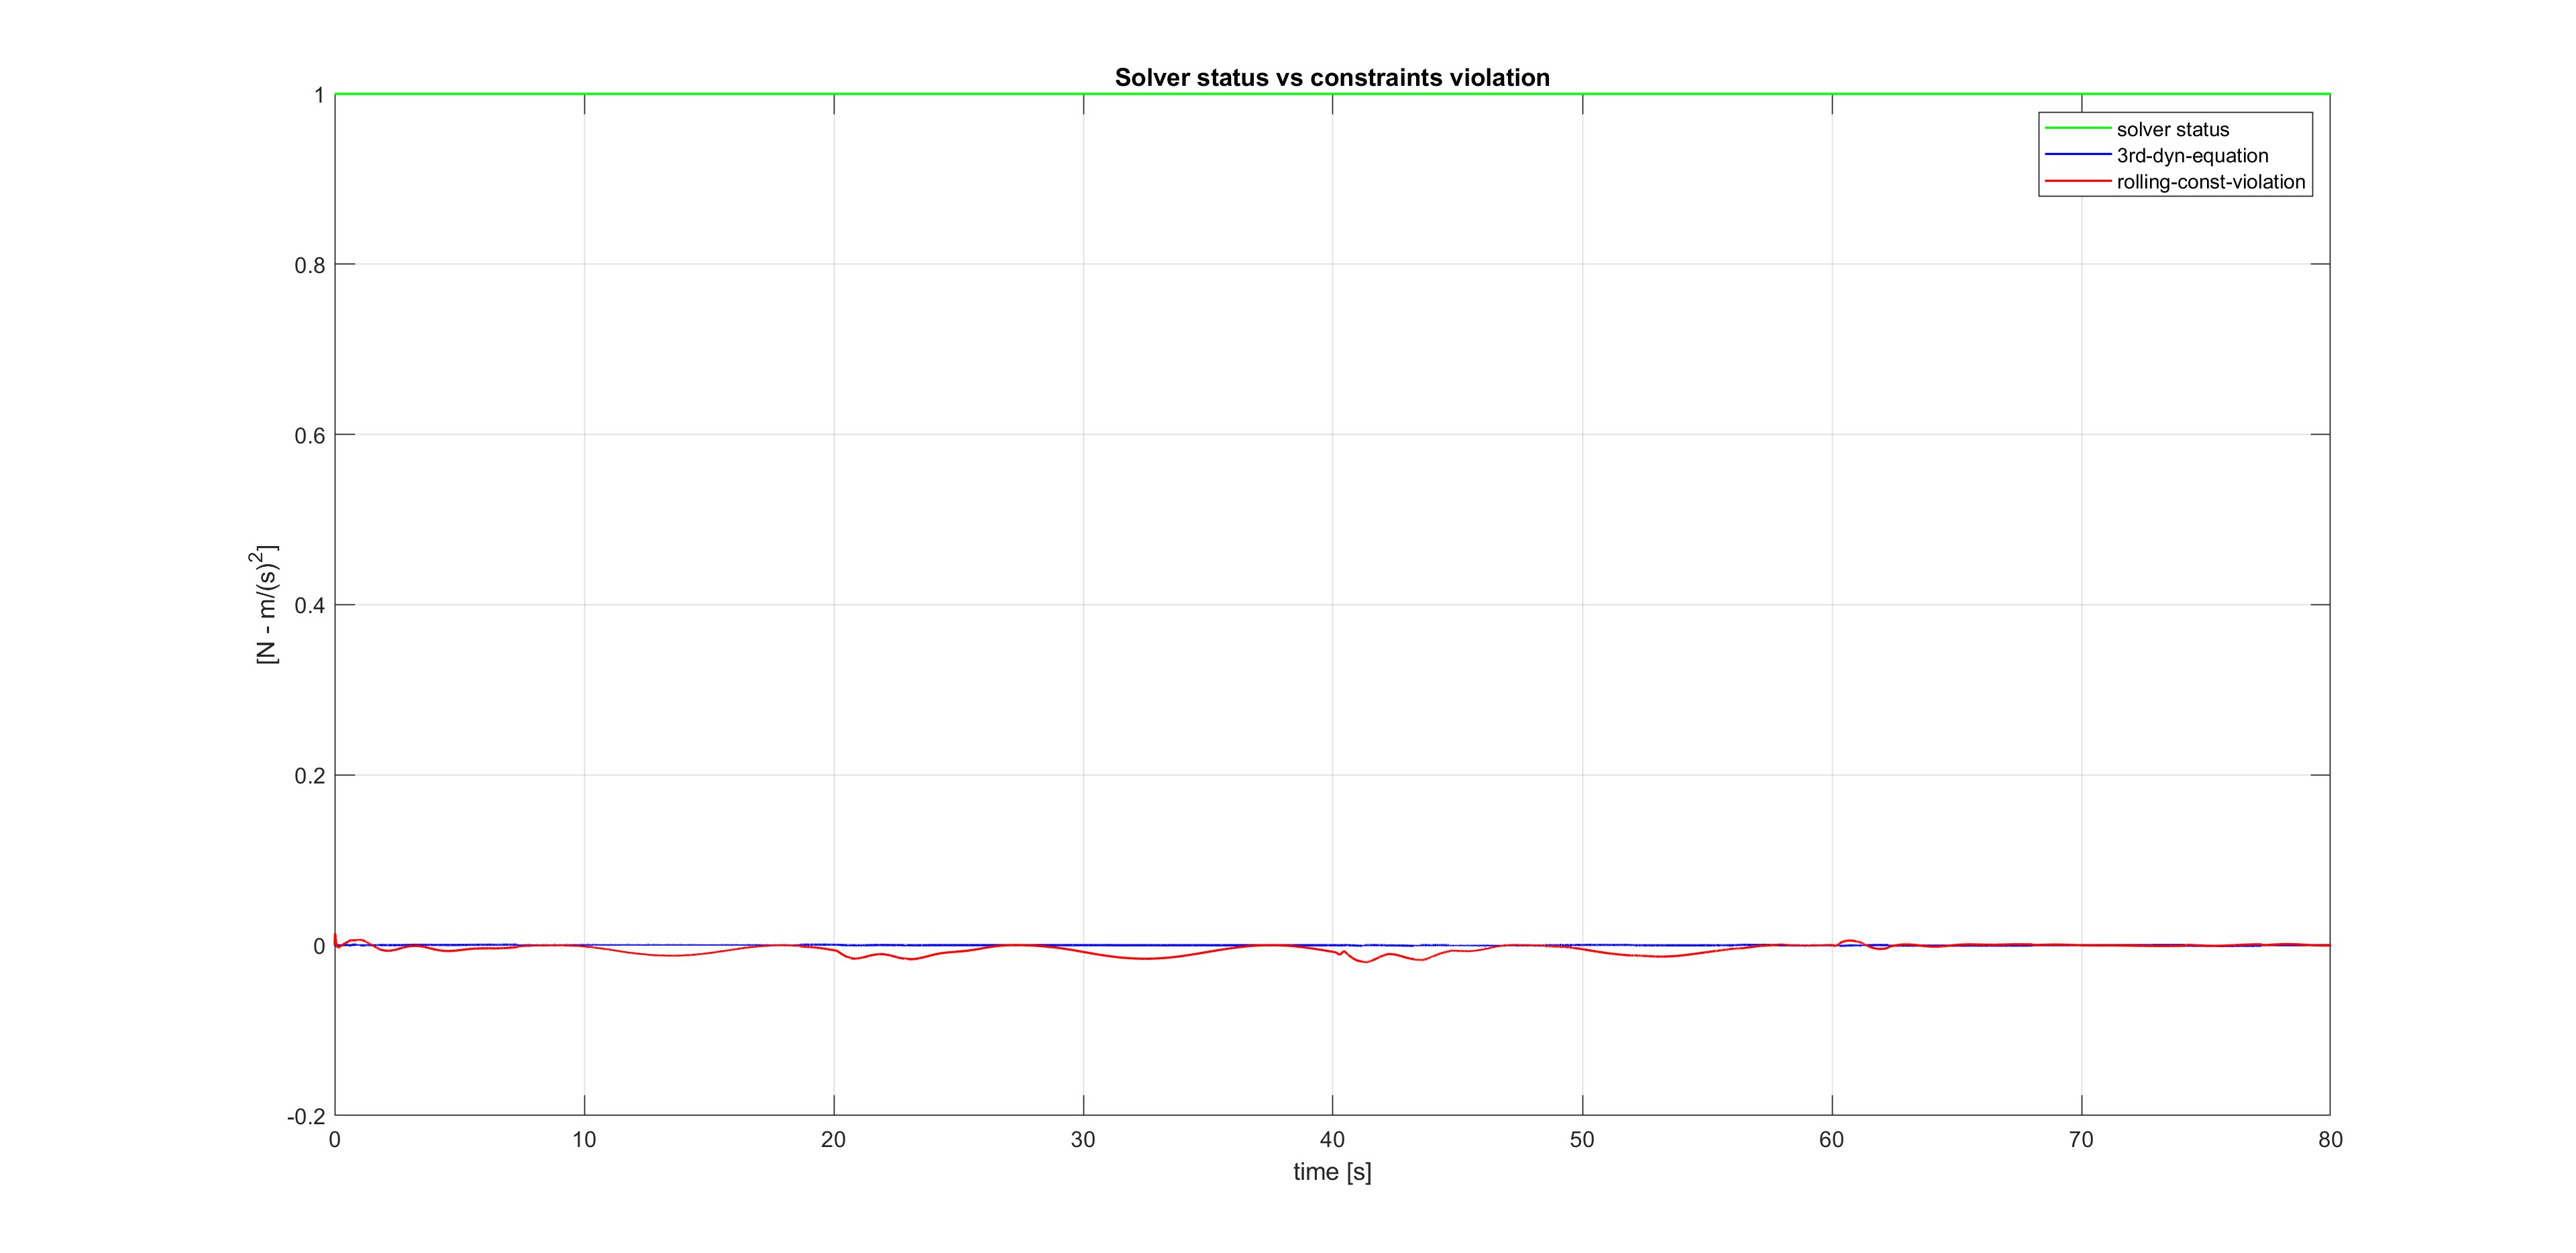
\includegraphics[width=1\linewidth]{Images/Robustness analysis/maximum load/sinusoidal trajectory/Slipping_velocity.jpg}
    \caption{Sinusoidal trajectory slipping velocity with disturbances in the case of maximum load.}
    \label{fig:Sinusoidal trajectory slipping velocity with disturbances in the case of maximum load}
\end{figure}

Figure \ref{fig:Sinusoidal trajectory slipping velocity with disturbances in the case of maximum load} instead shows how the solver never fails to provide a solution respecting the constraints.

\chapter{Conclusions and future developments}
\label{ch:conclusions}%

This thesis presents a new control strategy for a smart E-Cargo, belonging to a class of vehicles that can be identified under the name of \textit{two wheeled inverted pendulum}. The vehicle has been modeled as a floating base system and the control framework implemented is named Task Space Inverse Dynamics (TSID) and belongs to the big class of feedback linearization controllers.
With respect to the state of the art our controller solves a constrained optimization problem, where one of the constraints aims at preventing the slip between the wheels and the terrain. 
Since the actuators are modeled as torque sources, the controller's output consists of the two torques to be applied to each wheel.
We decided to implement a control in position on a point rigidly connected to the base, positioned 5 meters ahead of it, to desingularize the unicycle's in-plane configuration.
The self-balancing of the robot is then imposed inside the constraints, while the tracking of a reference trajectory is guaranteed as the minimization of the error dynamics.
A simple trajectory planner, constituted by a PI controller has been adopted to give the reference pitch angle, given the error in the in-plane velocity.
All the user-defined parameters have been defined through a trial and error approach, until we found an optimal set of controller gains and QP weights that works well in all the tested scenarios.
A first simulation has been performed considering the model as perfect without uncertainties and the E-Cargo loaded at its maximum load capacity of 60 kg: the plots show how both the swing-up and the trajectory are achieved with a very good performance and without violating anyone of the constraints.
A final robustness analysis has been carried out to test the controller performances with uncertainties in the model parameters and friction coefficient, considering three different loading conditions, maintaining the input URDF file constant.
The results achieved demonstrates how the controller is able to guarantee the initial swing up and the trajectory tracking even in the most undesired scenario in which the E-Cargo is loaded at its maximum capacity and has to start from the maximum allowed pitch angle.
Even if the results achieved until now are satisfying, there is still something that can be improved in order to achieve better performances and to make our assumptions more reasonable.
The strongest hypothesis that we made regards the knowledge of the friction coefficient between the wheels and the terrain, which is usually a wrong assumption in most of the cases.
Our preliminary solution intended to choose low values for this coefficient, in order to guarantee a proper functioning in most of the real case applications; a better approach can be the development of an estimator that based on the difference between the expected no-slip maximum velocity, and the actual one, decreases the friction coefficient in real time: if the estimate is fast enough we expect the controller to function properly.
Furthermore, a better trajectory planner can be implemented: instead of the linear PI controller, a Model Predictive Controller (MPC) can be used to calculate the optimal pitch trajectory according to the nominal trajectory that are imposed for the tracking task.
One final comment regard the possible implementation of an estimator for some model parameters like the CoM position or the total payload mass because, although we have demonstrated the robustness of the controller against the variation of these parameters, if we are able to know them with more precision, the performances can naturally improve.





%-------------------------------------------------------------------------
%	BIBLIOGRAPHY
%-------------------------------------------------------------------------

\addtocontents{toc}{\vspace{2em}} % Add a gap in the Contents, for aesthetics
\bibliography{Thesis_bibliography} % The references information are stored in the file named "Thesis_bibliography.bib"

%-------------------------------------------------------------------------
%	APPENDICES
%-------------------------------------------------------------------------

\cleardoublepage
\addtocontents{toc}{\vspace{2em}} % Add a gap in the Contents, for aesthetics
\appendix

\chapter{Appendix}
\label{ch:Appendix}%
% The \label{...}% enables to remove the small indentation that is generated, always leave the % symbol.

In this appendix, we derive several equations that, while pertinent to the understanding and implementation of concepts discussed in the main body of this thesis, are not the central focus of our investigation. These derivations provide additional information and technical details that contribute to a comprehensive understanding of the methodologies and principles employed.

A simplified notation is adopted for the following variables:

\begin{itemize}
    \item $\bm{\nu}$ indicates the mixed representation of the base generalized velocity $\bm{\nu}^{B[A]/B}$
    \item $J_{B}$ is the Jacobian of the base ${}^{B[A]} J_{A,B/B[A]}$
    \item $\mathbf{e_{3}}$ is the unitary vector $\begin{bmatrix}
        0 & 0 & 1 \\
    \end{bmatrix}^{T}$
\end{itemize}

\section{Self-Balancing equation}
\label{sec:Self-Balancing equation}

Here are provided just some mathematical passages to understand which are the element involved in Equation \eqref{eq: Pitch angular acceleration}.

Starting from Equation \eqref{eq:YRP Jacobian}, given the known elementary rotation matrices $R_{y}(\theta),R_{z}(\phi)$ \cite{Siciliano-et-al}, the final expression for the Jacobian is:

\begin{equation}
    {}^{A}J_{YRP} = \begin{bmatrix}
        \cos{\theta}\cos{\phi} & -\sin{\phi} & 0 \\
        sin{\phi} & cos{\phi} & 0 \\
        -sin{\theta}\cos{\phi} & 0 & 1 \\
    \end{bmatrix}
\end{equation}

where $\theta$ and $\phi$ are obtained (given the rotations sequence in Figure \ref{fig:Yaw-Roll-Pitch decomposition}) from the rotation matrix ${}^{A}R_{B}$ as

\begin{equation}
\begin{cases}
    \theta = \arctan_{2}(-{}^{A}R_{B}(3,1),\sqrt{({}^{A}R_{B}(3,2))^2+({}^{A}R_{B}(3,3))^2}) \\
    \psi = \arctan_{2}({}^{A}R_{B}(2,1),{}^{A}R_{B}(1,1)) 
    \end{cases}
\end{equation}


This Jacobian is invertible if its determinant is $\neq 0$, and so 

\begin{equation*}
    \cos{\theta}\cos{\phi}^{2} + \sin{\phi}^{2} \neq 0
\end{equation*}

Given this insight, if we define a selection matrix $S_{\omega}$


\begin{equation*}
    S_{\omega} = \begin{bmatrix}
 0 & 0 & 0 & 1 & 0 & 0 \\
 0 & 0 & 0 & 0 & 1 & 0 \\
 0 & 0 & 0 & 0 & 0 & 1 \\
\end{bmatrix}
\end{equation*}

and another selection matrix $S_{\theta}$

\begin{equation*}
    S_{\theta} = \begin{bmatrix}
 0 & 1 & 0 
\end{bmatrix}
\end{equation*}

Considering that we need the right trivialized base angular velocity ${}^{A}\bm{\omega}_{A,B}$

\begin{equation*}
  {}^{A}\bm{\omega}_{A,B} =  S_{\omega}J_{B}\bm{\nu}  
\end{equation*}

The final Equation \eqref{eq: Pitch angular acceleration} is obtained 

\begin{equation*}
    \ddot{\theta} = S_{\theta}{}^{A}J^{-1}_{YRP}S_{\omega}J_{B}\dot{\bm{\nu}} - S_{\theta}{}^{A}\dot{J}^{-1}_{YRP}S_{\omega}J_{B}\bm{\nu}
\end{equation*}

\section{Tracking equation}
\label{sec:Tracking equation}

Starting from Equation \eqref{eq:control point velocity}

\begin{equation*}
    {}^{A} \dot{\bm{\alpha}} = \frac{d}{dt} ({}^{A} \bm{\alpha}) = {}^{A} \dot{\mathbf{P}} + {}^{A} \dot{R}_B^{xy} {}^{B} \bm{\delta}
\end{equation*}

Let us define a selection matrix $S_{v_{\alpha}}$ as

\begin{equation*}
 S_{v_{\alpha}} = \begin{bmatrix}
 1 & 0 & 0 & 0 & 0 & 0 \\
 0 & 1 & 0 & 0 & 0 & 0 \\
\end{bmatrix}
\end{equation*}

the terms involved in equation \eqref{eq:control point velocity} are:

\begin{itemize}
    \item ${}^{A} \dot{\mathbf{P}}$ which includes the components x and y of the base velocity and can be written as: 
\begin{equation*}
    {}^{A} \dot{\mathbf{P}} = S_{v_{\alpha}}J_{B}\bm{\nu}
\end{equation*}

where $J_{B}$ is the Jacobian of the base, and so the product $S_{v_{\alpha}}J_{B}$ gives a matrix like:

\begin{equation*}
    \begin{bmatrix} 
        1 & 0 & 0 & 0 & 0 & 0 & 0 & 0 \\
        0 & 1 & 0 & 0 & 0 & 0 & 0 & 0 \\
    \end{bmatrix}
\end{equation*}

\item ${}^{A} \dot{R}^{xy}_{B} {}^{B} \bm{\delta}$ for which can be written:

\begin{equation*}
{}^{A} \dot{R}^{xy}_{B} = {}^{A}R^{xy}_{B} {}^{B}\bm{\omega}^{\wedge{}}_{A,B}
\end{equation*}


This term ${}^{B}\bm{\omega}^{\wedge{}}_{A,B}$ is the skewsimmetryc matrix of the vector ${}^{B}\bm{\omega}_{A,B}$ which is the angular velocity of the base given by:

\begin{equation*}
  {}^{B}\bm{\omega}_{A,B} =  {}^{B}R_{B[A]}S_{\omega}J_{B}\bm{\nu}  
\end{equation*}


\end{itemize}

Regarding the acceleration of the control point point $\ddot{\bm{\alpha}}$ its expression is:

\begin{equation*}
{}^{A}\ddot{\bm{\alpha}}_{xy} = \frac{d}{dt} [S_{v_{\alpha}}J_{B}\bm{\nu} + S_{v_{\alpha}}{}^{A}R^{xy}_{B} {}^{B}\bm{\omega}^{\wedge{}}_{A,B} {}^{B}\bm{\delta}] = \frac{d}{dt} [S_{v_{\alpha}}J_{B}\nu + S_{v_{\alpha}}{}^{A}R^{xy}_{B}({}^{B}R^{xy}_{B[A]}S_{\omega}J_{B} \bm{\nu})^{\wedge}{}^{B}\bm{\delta}]
\end{equation*}


Now exploiting the linear property of the cross product operator: $\mathbf{v}^{\wedge{}}\mathbf{x} = - \mathbf{x}^{\wedge{}}\mathbf{v}$

\begin{equation*}
{}^{A}R^{xy}_{B}({}^{B}R^{xy}_{B[A]}S_{\omega}J_{B} \bm{\nu})^{\wedge{}}{}^{B}\bm{\delta} = - {}^{A}R^{xy}_{B}({}^{B}\delta)^{\wedge{}}{}^{B}R^{xy}_{B[A]}S_{\omega}J_{B} \bm{\nu}
\end{equation*}

So we can obtain the final form of Equation \eqref{eq:control point acceleration affine} (considering that $J_{B}$ and the selection matrices are constant) as:

\begin{equation*}
\begin{aligned}
{}^{A} \ddot{\bm{\alpha}}_{xy} = & \; S_{v_{\alpha}}J_{B}\dot{\bm{\nu}} - S_{v_{\alpha}}{}^{A} \dot{R}^{xy}_{B} ({}^{B}\bm{\delta}) ^\wedge {}^{B}R^{xy}_{B[A]}S_{\omega}J_{B} \bm{\nu} \\
& - S_{v_{\alpha}}{}^{A} R^{xy}_{B}({}^{B}\bm{\delta})^\wedge {}^{A}\dot{R}^{xy}_{B[A]} S_{\omega}{}^{B} J_{B} \bm{\nu} - S_{v_{\alpha}}{}^{A} R^{xy}_{B}({}^{B}\bm{\delta})^\wedge {}^{B}R^{xy}_{B[A]} S_{\omega}J_{B} \dot{\bm{\nu}}
\end{aligned}
\label{eq:control point acceleration affine}
\end{equation*}

where: ${}^{A} \dot{R}^{xy}_{B} = {}^{A}R^{xy}_{B} {}^{B}\bm{\omega}^{\wedge{}}_{A,B}$ is the previously obtained term.
    
\section{Rolling equation}
\label{sec:Rolling equation}

In this section are reported some additional passages to express the rolling acceleration constraint in the form that the TSID needs:

The target is to arrive at a formulation in which the velocities and their derivatives are expressed as functions of $\bm{\nu}$ and $\dot{\bm{\nu}}$ such as the following.

\begin{equation}
{}^{L[A]}  \mathbf{v}_{A,L} = {}^{L[A]} J_{A,L/B[A]} \bm{\nu}^{B[A]/B}
\label{eq: wheel center velocity}
\end{equation}

where 

\begin{equation*}
    J_{L} =  {}^{L[A]} J_{A,L/B[A]}
\end{equation*}

Let us now define a selection matrix $S_{v}$ as

\begin{equation*}
 S_{v} = \begin{bmatrix}
 1 & 0 & 0 & 0 & 0 & 0 \\
 0 & 1 & 0 & 0 & 0 & 0 \\
 0 & 0 & 1 & 0 & 0 & 0 \\
\end{bmatrix}
\end{equation*}

What can be written is

$$  \begin{cases}
{}^{A} \dot{\mathbf{P}}_{L} = S_{v} J_{L}\bm{\nu} \\
{}^{A} \ddot{\mathbf{P}}_{L} = S_v J_{L}\dot{\bm{\nu}} + S_{v} \dot{J}_{L}\bm{\nu} \\
{}^{A} \bm{\omega}_{A,L} = S_{\omega} J_{L}\bm{\nu} \\
{}^{A} \dot{\bm{\omega}}_{A,L} = S_{\omega} J_L\dot{\bm{\nu}} + S_{\omega}  \dot{J}_{L} \bm{\nu} \\
\end{cases}$$

In this way, rearranging terms:

$$
S_{v} J_{L}\dot{\bm{\nu}} +  S_{v} \dot{J}_{L}\bm{\nu} = -r\mathbf{e_{3}}^{\wedge{}}[S_{\omega} J_{L}\dot{\bm{\nu}} + S_{\omega}  \dot{J}_{L} \bm{\nu}]$$ 

And so the final formulation that our controller requires is:

\begin{equation*}
 (S_{v} J_{L} + r\mathbf{e_{3}}^{\wedge{}} S_{\omega} J_{L}) \dot{\bm{\nu}} + (r\mathbf{e_{3}}^{\wedge{}} S_{\omega} + S_{v}) \dot{J}_{L} \bm{\nu} = 0
\end{equation*}

\section{Converting Least-Squares to Quadratic Programming}
\label{sec:Converting Least-Squares to Quadratic Programming}

Starting from the LSP formulation in \eqref{eq: LSP Formulation}

\begin{center}
$\underset{\bm{\dot{\nu},{}_{B}\mathbf{f},\bm{\tau}}}{\text{argmin}} (W_{\alpha}\|J_{T_{\alpha}}{\dot{\bm{\nu}}} - \dot{J}_{T_{\alpha}}\bm{\nu} - \ddot{\bm{\alpha}}_{xy}^{*}\|^{2} + w_{\tau}\| \tau_L \|^{2} + w_{\tau}\| \tau_R \|^{2} + w_{\xi} \| \xi \|^{2} + {}_{B}\mathbf{f}^{T} \lambda I {}_{B}\mathbf{f})$

\text{subject to}

\end{center}

\begin{equation*}
\begin{cases}
        M(\mathbf{q})\dot{\bm{\nu}} + h(\mathbf{q},\bm{\nu}) = S\bm{\tau} + J^{T}_{C} {}_{B}\mathbf{f} \\
        J_{R}\bm{\dot{\nu}} + \dot{J}_R\bm{\nu} = 0 \\
        J_{T_P}{\dot{\bm{\nu}}} - \dot{J}_{T_P}\bm{\nu} - \ddot{\theta}^{*} + \xi = 0 \\
        A_{f}{}_{B}\mathbf{f} < \mathbf{b}_{f} \\
        lb_{\xi} \leq \xi \leq ub_{\xi}
\end{cases}
\end{equation*}

we define the vector of optimization variables such as 

\begin{equation}
 \mathbf{v} = \begin{Bmatrix}
     \dot{\bm{\nu}} \\
     {}_{B}\mathbf{f} \\
     \bm{\tau}  \\
     \xi \\
\end{Bmatrix} \in \mathbb{R}^{17}
\end{equation}

A weighting matrix W such as

\begin{equation}
W = \begin{bmatrix}
w_{\alpha_x} & 0 & \cdots & 0 & 0 \\
0 & w_{\alpha_y} & \cdots & 0 & 0 \\
\vdots & \vdots & \ddots & \vdots & \vdots \\
0 & 0 & \cdots &  \ddots & 0 \\
0 & 0 & \cdots & 0 & w_{\xi}
\end{bmatrix} \in \mathbb{R}^{5 \times 5}
\end{equation}

And a regulariztion matrix such as

\begin{equation}
\lambda I = \begin{bmatrix}
0 & \cdots & \cdots & 0 & 0 \\
0 & \ddots & \cdots & 0 & 0 \\
\vdots & \vdots & \lambda I_{6 \times 6} & \vdots & \vdots \\
0 & 0 & \cdots & \ddots & 0 \\
0 & 0 & \cdots & 0 & 0 
\end{bmatrix} \in \mathbb{R}^{17 \times 17}
\end{equation}

The LS cost function can be written in a matrix form as $(\| D\mathbf{v} - \mathbf{a} \|^{2} + \mathbf{v}^{T} \lambda I \mathbf{v})$  which can be expanded as

\begin{equation*}
    (D\mathbf{v} - \mathbf{a})^{T}(D\mathbf{v} - \mathbf{a}) + \mathbf{v}^{T} \lambda I \mathbf{v}=
\end{equation*}

\begin{equation*}
   = (\mathbf{v}^{T} D^{T} D \mathbf{v} - 2\mathbf{a}^{T}D\mathbf{v} +\frac{1}{2} \mathbf{a}^{T}\mathbf{a} + \mathbf{v}^{T} \lambda I \mathbf{v}) =
\end{equation*}

\begin{equation*}
   = (\frac{1}{2} \mathbf{v}^{T} D^{T} D \mathbf{v} - \mathbf{a}^{T}D\mathbf{v} + \mathbf{a}^{T}\mathbf{a} + \frac{1}{2} \mathbf{v}^{T} \lambda I \mathbf{v}) =
\end{equation*}

Now defining a new matrix
\begin{equation*}
  H = D^{T} D + \lambda I 
\end{equation*}

and a new vector 
\begin{equation*}
  \mathbf{c} = \mathbf{a}^{T}D
\end{equation*}

considering that the term $(\mathbf{a}^{T}\mathbf{a})$ does not depend on the optimization variables, and so does not influence the optimization problem, the LS cost function in \eqref{eq: LSP Formulation} can be written as the one in \eqref{eq: QP Formulation}

\begin{center}
$\underset{\bm{\dot{\nu},{}_{B}\mathbf{f},\bm{\tau}}, \bm{\xi}}{\text{argmin}} (\frac{1}{2} \mathbf{v}^{T} H \mathbf{v} + \mathbf{c}^{T} \mathbf{v})$
\end{center}

for what concerns the constraints in \eqref{eq: LSP Formulation}, they can be rewritten in a matrix form as 


\begin{equation}
\begin{Bmatrix} 
-h(\mathbf{q},\bm{\nu})\\
-\dot{J_{R}}\bm{\nu} \\
\dot{J}_{T_P}\bm{\nu} + \ddot{\theta}^{*}\\
-\bm{\infty} \\
ub_{\xi} \\
\end{Bmatrix} \leq \begin{bmatrix} 
M(\mathbf{q}) & -J_c^{T} & -S & 0 \\
J_{R} & 0 & 0  & 0\\
J_{T_P} & 0 & 0  & 1\\
0 & A_{f} & 0 & 0\\
0 & 0 & 0 & 1 \\
\end{bmatrix} \begin{Bmatrix} 
\dot{\bm{\nu}} \\
{}_{B}\mathbf{f} \\
\bm{\tau}  \\
\xi \\
\end{Bmatrix} \leq \begin{Bmatrix} 
-h(\mathbf{q},\bm{\nu})\\\
-\dot{J_{R}}\bm{\nu}\\
\dot{J}_{T_P}\bm{\nu} + \ddot{\theta}^{*} \\
\mathbf{b}_{f} \\
ub_{\xi} \\
\end{Bmatrix}
\end{equation}

and then condensed in a more compact formulation

\begin{equation*}
    \mathbf{l}_b \leq A \mathbf{v} \leq \mathbf{u}_b
\end{equation*}

In this way we get to the final QP formulation given in Equation\eqref{eq: QP Formulation} 

\vspace{12pt}
\begin{center}
{\large \textbf{QP Formulation}}
\end{center}

\begin{center}
$\underset{\bm{\dot{\nu},{}_{B}\mathbf{f},\bm{\tau}}, \bm{\xi}}{\text{argmin}} (\frac{1}{2} \mathbf{v}^{T} H \mathbf{v} + \mathbf{c}^{T} \mathbf{v})$

\text{subject to}

\end{center}
\begin{equation*}
\mathbf{l}_b \leq A \mathbf{v} \leq \mathbf{u}_b
\end{equation*}


% LIST OF FIGURES
\listoffigures

% LIST OF TABLES
\listoftables

% ACKNOWLEDGEMENTS

\chapter{Ringraziamenti}
\label{ch:Ringraziamenti}

Vorrei a questo punto spendere qualche parola per ringraziare tutte le persone che direttamente o indirettamente sono state parte di questo viaggio ed hanno contribuito ai risultati che ho raggiunto.
Inizio dal ringraziare l'Istituto Italiano di Tecnologia ed in particolare Daniele Pucci per avermi accolto in questa grande famiglia, dandomi la possibilità di vivere un'esperienza bellissima.
Un grazie anche a tutto il dipartimento di Artificial Mechanical Intelligence, in particolare a Silvio, Stefano e Giorgio che con la massima pazienza e professionalità mi hanno insegnato ad affrontare e risolvere i problemi (anche quelli impossibili).
Grazie anche ovviamente a tutti gli altri ragazzi di AMI, perché nemmeno nella più rosea delle aspettative avrei immaginato di trovare degli amici oltre che colleghi.

Ringrazio il Politecnico di Milano ed il Prof. Francesco Braghin, sempre disponibile e presente durante tutto il mio lavoro.

Approfitto di questa occasione per ringraziare la mia famiglia iniziando dai miei genitori Sergio e Maria Antonietta, consapevole che non basterebbe un'altra tesi di laurea per descrivere quanto sono stato fortunato.
Da quando sono piccolo hanno sempre camminato dietro di me, lasciando che fossi io a decidere la strada, non troppo vicini per farmi sentire libero, ma nemmeno troppo lontani per essere pronti ad aiutarmi se cadevo: questo percorso mi ha fatto crescere e sono fiero dell'uomo che sono diventato perché somiglio a voi.

Insieme ai miei genitori ringrazio mio fratello Enrico, nonostante i caratteri diversi, abituarmi a vivere in una camera da solo è stata una delle sfide più difficili da affrontare, ma so che nonostante la distanza ci saremo sempre l'uno per l'altro.

Grazie ai miei nonni Angelo, Emilia, Iolanda e Tonino: i professori mi hanno insegnato a risolvere le equazioni, ma voi mi avete insegnato a leggere e contare, anche se non vi chiamo spesso, siete sempre con me.

Ringrazio i miei zii Fausto e Irene e mio cugino Augusto, siete sempre stati la mia seconda famiglia, il rifugio quando facevo arrabbiare mamma e papà, perché la regola che valeva era: "quando ci sono gli zii Davide può fare tutto".

Un ultimo ringraziamento infine a tutti i miei amici: da quelli che mi conoscono da sempre e sono sempre stati presenti durante tutto il mio percorso, a quelli che sono entrati e poi usciti perché la vita è strana, per finire con quelli che ci sono da poco, ma non per questo meno importanti.
Tutti mi avete lasciato qualcosa di vostro e spero anche io di aver lasciato qualcosa di mio a voi, con alcuni ho condiviso i momenti più belli e più brutti della mia vita, sappiate che non me ne dimenticherò mai.



\begin{flushright}
Con affetto,
Davide
\end{flushright}

\cleardoublepage

\clearpage
\thispagestyle{empty}
\mbox{}

\end{document}
